\documentclass[twoside]{book}

% Packages required by doxygen
\usepackage{calc}
\usepackage{doxygen}
\usepackage{graphicx}
\usepackage[utf8]{inputenc}
\usepackage{makeidx}
\usepackage{multicol}
\usepackage{multirow}
\usepackage{textcomp}
\usepackage[table]{xcolor}

% Font selection
\usepackage[T1]{fontenc}
\usepackage{mathptmx}
\usepackage[scaled=.90]{helvet}
\usepackage{courier}
\usepackage{amssymb}
\usepackage{sectsty}
\renewcommand{\familydefault}{\sfdefault}
\allsectionsfont{%
  \fontseries{bc}\selectfont%
  \color{darkgray}%
}
\renewcommand{\DoxyLabelFont}{%
  \fontseries{bc}\selectfont%
  \color{darkgray}%
}

% Page & text layout
\usepackage{geometry}
\geometry{%
  a4paper,%
  top=2.5cm,%
  bottom=2.5cm,%
  left=2.5cm,%
  right=2.5cm%
}
\tolerance=750
\hfuzz=15pt
\hbadness=750
\setlength{\emergencystretch}{15pt}
\setlength{\parindent}{0cm}
\setlength{\parskip}{0.2cm}
\makeatletter
\renewcommand{\paragraph}{%
  \@startsection{paragraph}{4}{0ex}{-1.0ex}{1.0ex}{%
    \normalfont\normalsize\bfseries\SS@parafont%
  }%
}
\renewcommand{\subparagraph}{%
  \@startsection{subparagraph}{5}{0ex}{-1.0ex}{1.0ex}{%
    \normalfont\normalsize\bfseries\SS@subparafont%
  }%
}
\makeatother

% Headers & footers
\usepackage{fancyhdr}
\pagestyle{fancyplain}
\fancyhead[LE]{\fancyplain{}{\bfseries\thepage}}
\fancyhead[CE]{\fancyplain{}{}}
\fancyhead[RE]{\fancyplain{}{\bfseries\leftmark}}
\fancyhead[LO]{\fancyplain{}{\bfseries\rightmark}}
\fancyhead[CO]{\fancyplain{}{}}
\fancyhead[RO]{\fancyplain{}{\bfseries\thepage}}
\fancyfoot[LE]{\fancyplain{}{}}
\fancyfoot[CE]{\fancyplain{}{}}
\fancyfoot[RE]{\fancyplain{}{\bfseries\scriptsize Generated on Tue Nov 10 2015 18\-:29\-:07 for Payload by Doxygen }}
\fancyfoot[LO]{\fancyplain{}{\bfseries\scriptsize Generated on Tue Nov 10 2015 18\-:29\-:07 for Payload by Doxygen }}
\fancyfoot[CO]{\fancyplain{}{}}
\fancyfoot[RO]{\fancyplain{}{}}
\renewcommand{\footrulewidth}{0.4pt}
\renewcommand{\chaptermark}[1]{%
  \markboth{#1}{}%
}
\renewcommand{\sectionmark}[1]{%
  \markright{\thesection\ #1}%
}

% Indices & bibliography
\usepackage{natbib}
\usepackage[titles]{tocloft}
\setcounter{tocdepth}{3}
\setcounter{secnumdepth}{5}
\makeindex

% Hyperlinks (required, but should be loaded last)
\usepackage{ifpdf}
\ifpdf
  \usepackage[pdftex,pagebackref=true]{hyperref}
\else
  \usepackage[ps2pdf,pagebackref=true]{hyperref}
\fi
\hypersetup{%
  colorlinks=true,%
  linkcolor=blue,%
  citecolor=blue,%
  unicode%
}

% Custom commands
\newcommand{\clearemptydoublepage}{%
  \newpage{\pagestyle{empty}\cleardoublepage}%
}


%===== C O N T E N T S =====

\begin{document}

% Titlepage & ToC
\hypersetup{pageanchor=false}
\pagenumbering{roman}
\begin{titlepage}
\vspace*{7cm}
\begin{center}%
{\Large Payload }\\
\vspace*{1cm}
{\large Generated by Doxygen 1.8.6}\\
\vspace*{0.5cm}
{\small Tue Nov 10 2015 18:29:07}\\
\end{center}
\end{titlepage}
\clearemptydoublepage
\tableofcontents
\clearemptydoublepage
\pagenumbering{arabic}
\hypersetup{pageanchor=true}

%--- Begin generated contents ---
\chapter{Payload\-G\-U\-I}
\label{md_BaseStation_PayloadGUI_README}
\hypertarget{md_BaseStation_PayloadGUI_README}{}
This is the G\-U\-I for controlling the payload system; this includes the camera, network, A\-D\-L\-C and browsing of uploaded images.

\section*{Files }

$\ast$$\ast$$\ast$main.cpp$\ast$$\ast$$\ast$ --- Main program file

$\ast$$\ast$$\ast$\-Main\-Window.cpp/h$\ast$$\ast$$\ast$ --- Priamry window that all the other widgets dock into.

{\bfseries \hyperlink{CameraWidget_8cpp}{Camera\-Widget.\-cpp}/h} --- Widget for controlling the camera.

{\bfseries \hyperlink{NetworkWidget_8cpp}{Network\-Widget.\-cpp}/h} --- Widget for controlling the network.

{\bfseries Pyload\-G\-U\-I.\-pro} --- Configuration file for qmake. If any additional classes are created, append the .cpp to this file.

{\bfseries M\-A\-K\-E\-F\-I\-L\-E} --- Makefile generated by qmake. If Payload\-G\-U\-I.\-pro is modified run qmake to regenerate.\-kj 
\chapter{Base\-Station}
\label{md_BaseStation_README}
\hypertarget{md_BaseStation_README}{}
This directory contains all of the code for the base station, including the Base\-Station\-Comms A\-D\-L\-C and the Payload\-G\-U\-I.

{\bfseries Base\-Station\-Comms} --- Establishes and maintains a network connection between the Base Station and the Payload. Tracks changes from the Payload\-G\-U\-I and transmits packets to the payload. Also accepts incoming packets from the payload and alerts the Payload\-G\-U\-I.

{\bfseries Payload\-G\-U\-I} --- The main interface for controlling the payload. Gives the user an intuitive graphical interface with which to establish a network connection and control critical payload functionality such as starting camera capture and A\-D\-L\-C. Also has the capability to scan through the images transmitted back to the Base Station.

{\bfseries A\-D\-L\-C} --- All of the image processing code running on the base station.

{\bfseries Base Station Class Diagram} 

{\bfseries Star Packet Inheritance Tree}

 
\chapter{R\-E\-A\-D\-M\-E}
\label{md_Payload_ADLC_README}
\hypertarget{md_Payload_ADLC_README}{}
This file contains code to complete A\-D\-L\-C task specified in the A\-U\-V\-S\-I rules\-:

7.\-3. A\-U\-T\-O\-M\-A\-T\-I\-C D\-E\-T\-E\-C\-T\-I\-O\-N, L\-O\-C\-A\-L\-I\-Z\-A\-T\-I\-O\-N, A\-N\-D C\-L\-A\-S\-S\-I\-F\-I\-C\-A\-T\-I\-O\-N (A\-D\-L\-C) T\-A\-S\-K (S\-E\-C\-O\-N\-D\-A\-R\-Y) Table 4\-:  \-A\-D\-L\-C Parameters Parameter Threshold Objective Automatic Localization (each target, standard, and Q\-R\-C) n/a Identify target position within 150 ft. Automatic Classification (each standard target) n/a Identify at least three of five target characteristics. Automatic Classification (each Q\-R\-C target) n/a Decode the message. False Alarm Rate (F\-A\-R) on Classification n/a Demonstrate $<$50\% F\-A\-R.

7.\-3.\-1. Teams shall develop an algorithm which performs automated detection of potential targets and cues the imagery judge.\-  \-The algorithm shall localize the detected targets and automatically determine the target characteristics.

7.\-3.\-2. Credit will be given for each target automatically detected \& cued, up to six targets.

7.\-3.\-3. A\-D\-L\-C may be performed by any combination of airborne or ground‐based processing.

7.\-3.\-4. Teams shall make their A\-D\-L\-C process very clear to the imagery judge prior to aircraft takeoff. 7.\-3.\-4.\-1. If a judge is unclear about or suspects manual assistance to the A\-D\-L\-C process, the team shall not receive A\-D\-L\-C task points.

7.\-3.\-5. Demonstrating an A\-D\-L\-C target 7.\-3.\-5.\-1. A\-L\-L automatic detections shall be clearly shown to the imagery judge without human interaction (e.\-g. a pop‐up window).    7.\-3.\-5.\-2. The first six detections shown shall be considered a team’s entry for the A\-D\-L\-C task.\-  \-These detections shall be turned into the judges by filling out a single dedicated target information sheet, given in Appendix E. This target information sheet shall be marked clearly with “\-Automatic Detections” and handed in separate from other imagery sheets. or provided electronically in accordance with Appendix D, and clearly marked in tab 11 as “\-Auto Detection

7.\-3.\-6. False Alarm Rate 7.\-3.\-6.\-1. If a listed target fails to meet the objective for classification, the target will be considered a false detection.\-  \-The number of incorrect A\-D\-L\-C targets reported will be divided by the total number of A\-D\-L\-C targets reported to determine false alarm rate. 7.\-3.\-6.\-2. Each detection/target is counted once.\-  \-If the false alarm rate exceeds the objective limit, no credit will be given for the A\-D\-L\-C task 
\chapter{Description}
\label{md_Payload_ADLC_SalientDetection_README}
\hypertarget{md_Payload_ADLC_SalientDetection_README}{}
This folder contains the code for region of interest detection and cropping.

It is a salient object detection method that uses a sobel filter of the u$\ast$ and v$\ast$ channels of the Lu$\ast$v$\ast$ color space.

\section*{Action/result chart\-: }

image input $\vert$ $\vert$ cropped regions of interest output

This is just showing how the code will work for testing purposes.

\section*{Algorithm description }

convert to L\-U\-V colorspace $\vert$ $\vert$ gaussian filter $\vert$ $\vert$ Sobel filter $\vert$ $\vert$ gaussian filter $\vert$ $\vert$ image normalization $\vert$ $\vert$ Thresholding $\vert$ $\vert$ dilation $\vert$ $\vert$ Countours $\vert$ $\vert$ Counter boxing $\vert$ $\vert$ Box size filtering

\section*{Whats been done }

-\/\-Code has been implemented

-\/\-Basic testing has been done

\section*{T\-O\-D\-O }

-\/test the algorithm

-\/optimize the algorithm (gpu?)

\section*{Files in folder }

\hyperlink{salient__detection_8cpp}{salient\-\_\-detection.\-cpp} -\/ this is the main file that needs to be run

I\-M\-G\-\_\-0494/0526 -\/ test images that the code uses to crop

cropped\-Img -\/ the file where detected roi of interest are saved

competition\-Photos -\/ the folder that contains the test data set of photos taken during previous competitions

\section*{How to run }

cmake C\-Make\-Lists.\-txt

make

./salient\-\_\-det

\section*{Requirements }

most recent version of cmake

opencv version 2.\-4.\-10 
\chapter{Description}
\label{md_Payload_ADLC_ShapeCharacterization_README}
\hypertarget{md_Payload_ADLC_ShapeCharacterization_README}{}
This folder contains python scripts that are meant to test parts of a shape detection algorithm I am working on.

The alogrithm assumes potential targets have already been cropped. The end functionalilty will scan all of these images and only return the ones that have ground targets in them. This will comply with all standards that are stated in the A\-U\-V\-S\-I rules for the A\-D\-L\-C task. These scripts are compiled using the python 2.\-7 on windows with opencv 2.\-4.\-10 (the current stable version)

\section*{Action/result chart\-: }

cropped images input $\vert$ \subsection*{$\vert$ }

$\vert$ $\vert$ $\vert$ $\vert$ \hyperlink{structTarget}{Target} detected no target detected $\vert$ $\vert$ $\vert$ $\vert$ images saved return to start

This is just showing how the code will work for testing purposes.

\section*{Algorithm description }

The algorithm will consist of three parts\-:

-\/\-Image preprocessing \begin{DoxyVerb}            -First we segment the image into 3 three different colors

            -the next step is to convert the image to the luv color space

            -Next we sum the u* and  v* channels together

            -Then we use a sobel filter to find changes in color

            -next we use canny edge detection

              -This will allow the detector to detect the geometry of the target. If features arent drawn from the canny image then
              the surf features will detect the intensity of the image. This is not the point of the algorithm. The algorithm is only 
              meant to detect shapes not color.
\end{DoxyVerb}


-\/surf feature detection \begin{DoxyVerb}            -just uses opencv's surf library

              -should be faster than sift
\end{DoxyVerb}


-\/machine learning portion \begin{DoxyVerb}            -still doing research on this portion going to try to impliment three types

              -FLANN matching: currently being developed

                link: http://bit.ly/1tH9a6P

              -knn

                link: http://bit.ly/1vzLlba

              -svm

                link: http://bit.ly/1HjINq4
\end{DoxyVerb}


\section*{Whats been done }

-\/completed and tested surf feature detection

-\/completed and tested the preproccing method

-\/started implimenting flann matching

\section*{T\-O\-D\-O }

-\/impliment knn/svm detection

\section*{Files in folder }

Matching-\/1\-: basic flann implementation still under development

mean\-Clust-\/1\-: implementation/test of prepocessing algorithm \begin{DoxyVerb}            -outputs the clustered image and edges detected from that image
\end{DoxyVerb}


surf\-\_\-det-\/1\-: implementation/test of surf detector \begin{DoxyVerb}            -shows the feautures being detected in the preprocessed image\end{DoxyVerb}
 
\chapter{Payload}
\label{md_README}
\hypertarget{md_README}{}
This folder contains all code for the U\-A\-V payload, the base station code for controling the payload, and testing data sets.

\section*{Payload functionalites\-: }

-\/\-A\-D\-L\-C\-: Will allow the U\-A\-S to automatically detect, characterize, and localize ground targets without any human intervention.

-\/\-I\-M\-A\-G\-E P\-A\-S\-S T\-H\-R\-O\-U\-G\-H\-: will allow for images to be passed directly from the camera to the ground station without any object detection algorithms being run on it. This will allow for completion of the emergent and off axis target identification.

-\/\-S\-R\-I\-C\-: will allow for the uav to connect to a remote intelligence center and retreive data that is on the server.

\section*{Folders\-: }

All folders should contain the following information for future teams

-\/\-Code for subsystem

-\/f\-Subsystem test procedures

-\/\-Test results

-\/\-Test analysis

\section*{Code header\-: }

Please include a header with this format\-:

/$\ast$ Name\-: $<$ your name $>$

Date\-: $<$ date of last modification $>$

Functionality\-: $<$ what does it do $>$

Version\-: $<$ Version \# $>$

Changes log\-: $<$ changes since preious version $>$ 
\chapter{T\-O D\-O}
\label{md_TODO}
\hypertarget{md_TODO}{}
-\/\-Complete shape detection code

-\/\-Complete the state machine framework

-\/test camera \begin{DoxyVerb}-find the maximum velocity we can travel before the blur is to much

-test resolution
\end{DoxyVerb}


-\/\-Complete letter detection code

-\/complete color detection code

-\/test salient detection on all images

-\/implement the S\-R\-I\-C subsystem 
\chapter{Hierarchical Index}
\section{Class Hierarchy}
This inheritance list is sorted roughly, but not completely, alphabetically\-:\begin{DoxyCompactList}
\item \contentsline{section}{Base\-Station\-Comms\-Exec}{\pageref{classBaseStationCommsExec}}{}
\item \contentsline{section}{D\-D\-M\-Params}{\pageref{structDDMParams}}{}
\item \contentsline{section}{Dimage}{\pageref{classDimage}}{}
\item \contentsline{section}{Network}{\pageref{classNetwork}}{}
\item \contentsline{section}{Obd\-Image}{\pageref{classObdImage}}{}
\item \contentsline{section}{Obd\-Object}{\pageref{classObdObject}}{}
\item \contentsline{section}{Obd\-Score\-Index\-Sorter}{\pageref{classObdScoreIndexSorter}}{}
\item \contentsline{section}{Voc\-Data\-:\-:ordering\-Sorter}{\pageref{structVocData_1_1orderingSorter}}{}
\item \contentsline{section}{Packet\-Framer}{\pageref{classPacketFramer}}{}
\item \contentsline{section}{Packet\-Monitor}{\pageref{classPacketMonitor}}{}
\item \contentsline{section}{Payload\-Status}{\pageref{classPayloadStatus}}{}
\item Q\-Dock\-Widget\begin{DoxyCompactList}
\item \contentsline{section}{Camera\-Widget}{\pageref{classCameraWidget}}{}
\item \contentsline{section}{Network\-Widget}{\pageref{classNetworkWidget}}{}
\end{DoxyCompactList}
\item Q\-Main\-Window\begin{DoxyCompactList}
\item \contentsline{section}{Main\-Window}{\pageref{classMainWindow}}{}
\end{DoxyCompactList}
\item \contentsline{section}{Salient}{\pageref{classSalient}}{}
\item \contentsline{section}{Star\-Packet}{\pageref{classStarPacket}}{}
\begin{DoxyCompactList}
\item \contentsline{section}{Star\-Packet0x01}{\pageref{classStarPacket0x01}}{}
\item \contentsline{section}{Star\-Packet0x02}{\pageref{classStarPacket0x02}}{}
\item \contentsline{section}{Star\-Packet0x03}{\pageref{classStarPacket0x03}}{}
\end{DoxyCompactList}
\item \contentsline{section}{S\-V\-M\-Train\-Params\-Ext}{\pageref{structSVMTrainParamsExt}}{}
\item \contentsline{section}{Target}{\pageref{structTarget}}{}
\item \contentsline{section}{Vocab\-Train\-Params}{\pageref{structVocabTrainParams}}{}
\item \contentsline{section}{Voc\-Data}{\pageref{classVocData}}{}
\item \contentsline{section}{Voc\-Object\-Data}{\pageref{classVocObjectData}}{}
\end{DoxyCompactList}

\chapter{Class Index}
\section{Class List}
Here are the classes, structs, unions and interfaces with brief descriptions\-:\begin{DoxyCompactList}
\item\contentsline{section}{\hyperlink{classBaseStationCommsExec}{Base\-Station\-Comms\-Exec} }{\pageref{classBaseStationCommsExec}}{}
\item\contentsline{section}{\hyperlink{classCameraWidget}{Camera\-Widget} }{\pageref{classCameraWidget}}{}
\item\contentsline{section}{\hyperlink{structDDMParams}{D\-D\-M\-Params} }{\pageref{structDDMParams}}{}
\item\contentsline{section}{\hyperlink{classDimage}{Dimage} }{\pageref{classDimage}}{}
\item\contentsline{section}{\hyperlink{classMainWindow}{Main\-Window} \\*The main window for this application }{\pageref{classMainWindow}}{}
\item\contentsline{section}{\hyperlink{classNetwork}{Network} }{\pageref{classNetwork}}{}
\item\contentsline{section}{\hyperlink{classNetworkWidget}{Network\-Widget} }{\pageref{classNetworkWidget}}{}
\item\contentsline{section}{\hyperlink{classObdImage}{Obd\-Image} }{\pageref{classObdImage}}{}
\item\contentsline{section}{\hyperlink{classObdObject}{Obd\-Object} }{\pageref{classObdObject}}{}
\item\contentsline{section}{\hyperlink{classObdScoreIndexSorter}{Obd\-Score\-Index\-Sorter} }{\pageref{classObdScoreIndexSorter}}{}
\item\contentsline{section}{\hyperlink{structVocData_1_1orderingSorter}{Voc\-Data\-::ordering\-Sorter} }{\pageref{structVocData_1_1orderingSorter}}{}
\item\contentsline{section}{\hyperlink{classPacketFramer}{Packet\-Framer} }{\pageref{classPacketFramer}}{}
\item\contentsline{section}{\hyperlink{classPacketMonitor}{Packet\-Monitor} }{\pageref{classPacketMonitor}}{}
\item\contentsline{section}{\hyperlink{classPayloadStatus}{Payload\-Status} }{\pageref{classPayloadStatus}}{}
\item\contentsline{section}{\hyperlink{classSalient}{Salient} }{\pageref{classSalient}}{}
\item\contentsline{section}{\hyperlink{classStarPacket}{Star\-Packet} }{\pageref{classStarPacket}}{}
\item\contentsline{section}{\hyperlink{classStarPacket0x01}{Star\-Packet0x01} }{\pageref{classStarPacket0x01}}{}
\item\contentsline{section}{\hyperlink{classStarPacket0x02}{Star\-Packet0x02} }{\pageref{classStarPacket0x02}}{}
\item\contentsline{section}{\hyperlink{classStarPacket0x03}{Star\-Packet0x03} }{\pageref{classStarPacket0x03}}{}
\item\contentsline{section}{\hyperlink{structSVMTrainParamsExt}{S\-V\-M\-Train\-Params\-Ext} }{\pageref{structSVMTrainParamsExt}}{}
\item\contentsline{section}{\hyperlink{structTarget}{Target} }{\pageref{structTarget}}{}
\item\contentsline{section}{\hyperlink{structVocabTrainParams}{Vocab\-Train\-Params} }{\pageref{structVocabTrainParams}}{}
\item\contentsline{section}{\hyperlink{classVocData}{Voc\-Data} }{\pageref{classVocData}}{}
\item\contentsline{section}{\hyperlink{classVocObjectData}{Voc\-Object\-Data} }{\pageref{classVocObjectData}}{}
\end{DoxyCompactList}

\chapter{File Index}
\section{File List}
Here is a list of all files with brief descriptions\-:\begin{DoxyCompactList}
\item\contentsline{section}{Base\-Station/\hyperlink{BaseStationExec_8cpp}{Base\-Station\-Exec.\-cpp} }{\pageref{BaseStationExec_8cpp}}{}
\item\contentsline{section}{Base\-Station/\hyperlink{BaseStationExec_8h}{Base\-Station\-Exec.\-h} }{\pageref{BaseStationExec_8h}}{}
\item\contentsline{section}{Base\-Station/\-A\-D\-L\-C/inc/\hyperlink{BaseStation_2ADLC_2inc_2Dimage_8h}{Dimage.\-h} }{\pageref{BaseStation_2ADLC_2inc_2Dimage_8h}}{}
\item\contentsline{section}{Base\-Station/\-A\-D\-L\-C/src/\hyperlink{Dimage_8cpp}{Dimage.\-cpp} }{\pageref{Dimage_8cpp}}{}
\item\contentsline{section}{Base\-Station/\-A\-D\-L\-C/src/\hyperlink{ADLC_2src_2main_8cpp}{main.\-cpp} }{\pageref{ADLC_2src_2main_8cpp}}{}
\item\contentsline{section}{Base\-Station/\-A\-D\-L\-C/src/\hyperlink{Salient_8cpp}{Salient.\-cpp} }{\pageref{Salient_8cpp}}{}
\item\contentsline{section}{Base\-Station/\-A\-D\-L\-C/src/\-C\-Make\-Files/2.\-8.\-12.\-2/\-Compiler\-Id\-C\-X\-X/\hyperlink{BaseStation_2ADLC_2src_2CMakeFiles_22_88_812_82_2CompilerIdCXX_2CMakeCXXCompilerId_8cpp}{C\-Make\-C\-X\-X\-Compiler\-Id.\-cpp} }{\pageref{BaseStation_2ADLC_2src_2CMakeFiles_22_88_812_82_2CompilerIdCXX_2CMakeCXXCompilerId_8cpp}}{}
\item\contentsline{section}{Base\-Station/\-Base\-Station\-Comms/\hyperlink{BaseStationCommsExec_8cpp}{Base\-Station\-Comms\-Exec.\-cpp} }{\pageref{BaseStationCommsExec_8cpp}}{}
\item\contentsline{section}{Base\-Station/\-Base\-Station\-Comms/\hyperlink{BaseStationCommsExec_8h}{Base\-Station\-Comms\-Exec.\-h} }{\pageref{BaseStationCommsExec_8h}}{}
\item\contentsline{section}{Base\-Station/\-Base\-Station\-Comms/\hyperlink{Network_8cpp}{Network.\-cpp} }{\pageref{Network_8cpp}}{}
\item\contentsline{section}{Base\-Station/\-Base\-Station\-Comms/\hyperlink{Network_8h}{Network.\-h} }{\pageref{Network_8h}}{}
\item\contentsline{section}{Base\-Station/\-Base\-Station\-Comms/\hyperlink{PacketFramer_8cpp}{Packet\-Framer.\-cpp} }{\pageref{PacketFramer_8cpp}}{}
\item\contentsline{section}{Base\-Station/\-Base\-Station\-Comms/\hyperlink{PacketFramer_8h}{Packet\-Framer.\-h} }{\pageref{PacketFramer_8h}}{}
\item\contentsline{section}{Base\-Station/\-Base\-Station\-Comms/\hyperlink{PacketMonitor_8cpp}{Packet\-Monitor.\-cpp} }{\pageref{PacketMonitor_8cpp}}{}
\item\contentsline{section}{Base\-Station/\-Base\-Station\-Comms/\hyperlink{PacketMonitor_8h}{Packet\-Monitor.\-h} }{\pageref{PacketMonitor_8h}}{}
\item\contentsline{section}{Base\-Station/\-Payload\-G\-U\-I/\hyperlink{CameraWidget_8cpp}{Camera\-Widget.\-cpp} }{\pageref{CameraWidget_8cpp}}{}
\item\contentsline{section}{Base\-Station/\-Payload\-G\-U\-I/\hyperlink{CameraWidget_8h}{Camera\-Widget.\-h} }{\pageref{CameraWidget_8h}}{}
\item\contentsline{section}{Base\-Station/\-Payload\-G\-U\-I/\hyperlink{PayloadGUI_2main_8cpp}{main.\-cpp} }{\pageref{PayloadGUI_2main_8cpp}}{}
\item\contentsline{section}{Base\-Station/\-Payload\-G\-U\-I/\hyperlink{MainWindow_8cpp}{Main\-Window.\-cpp} }{\pageref{MainWindow_8cpp}}{}
\item\contentsline{section}{Base\-Station/\-Payload\-G\-U\-I/\hyperlink{MainWindow_8h}{Main\-Window.\-h} }{\pageref{MainWindow_8h}}{}
\item\contentsline{section}{Base\-Station/\-Payload\-G\-U\-I/\hyperlink{NetworkWidget_8cpp}{Network\-Widget.\-cpp} }{\pageref{NetworkWidget_8cpp}}{}
\item\contentsline{section}{Base\-Station/\-Payload\-G\-U\-I/\hyperlink{NetworkWidget_8h}{Network\-Widget.\-h} }{\pageref{NetworkWidget_8h}}{}
\item\contentsline{section}{Payload/\-A\-D\-L\-C/\-Feature\-Extraction/\-Feature\-Extraction/\hyperlink{feature_01extraction_8cpp}{feature extraction.\-cpp} }{\pageref{feature_01extraction_8cpp}}{}
\item\contentsline{section}{Payload/\-A\-D\-L\-C/\-Feature\-Extraction/\-Feature\-Extraction/\hyperlink{feature__extraction_8cpp}{feature\-\_\-extraction.\-cpp} }{\pageref{feature__extraction_8cpp}}{}
\item\contentsline{section}{Payload/\-A\-D\-L\-C/\-Feature\-Extraction/\-Feature\-Extraction/\hyperlink{stdafx_8cpp}{stdafx.\-cpp} }{\pageref{stdafx_8cpp}}{}
\item\contentsline{section}{Payload/\-A\-D\-L\-C/\-Feature\-Extraction/\-Feature\-Extraction/\hyperlink{stdafx_8h}{stdafx.\-h} }{\pageref{stdafx_8h}}{}
\item\contentsline{section}{Payload/\-A\-D\-L\-C/\-Feature\-Extraction/\-Feature\-Extraction/\hyperlink{targetver_8h}{targetver.\-h} }{\pageref{targetver_8h}}{}
\item\contentsline{section}{Payload/\-A\-D\-L\-C/\-Feature\-Extraction/\-Feature\-Extraction/\-C\-Make\-Files/2.\-8.\-12.\-2/\-Compiler\-Id\-C\-X\-X/\hyperlink{Payload_2ADLC_2FeatureExtraction_2FeatureExtraction_2CMakeFiles_22_88_812_82_2CompilerIdCXX_2CMakeCXXCompilerId_8cpp}{C\-Make\-C\-X\-X\-Compiler\-Id.\-cpp} }{\pageref{Payload_2ADLC_2FeatureExtraction_2FeatureExtraction_2CMakeFiles_22_88_812_82_2CompilerIdCXX_2CMakeCXXCompilerId_8cpp}}{}
\item\contentsline{section}{Payload/\-A\-D\-L\-C/\-Salient\-Detection/\hyperlink{Payload_2ADLC_2SalientDetection_2Dimage_8h}{Dimage.\-h} }{\pageref{Payload_2ADLC_2SalientDetection_2Dimage_8h}}{}
\item\contentsline{section}{Payload/\-A\-D\-L\-C/\-Salient\-Detection/\hyperlink{Salient_8h}{Salient.\-h} }{\pageref{Salient_8h}}{}
\item\contentsline{section}{Payload/\-A\-D\-L\-C/\-Salient\-Detection/\hyperlink{salient__detection_8cpp}{salient\-\_\-detection.\-cpp} }{\pageref{salient__detection_8cpp}}{}
\item\contentsline{section}{Payload/\-A\-D\-L\-C/\-Salient\-Detection/\-C\-Make\-Files/2.\-8.\-12.\-2/\-Compiler\-Id\-C\-X\-X/\hyperlink{Payload_2ADLC_2SalientDetection_2CMakeFiles_22_88_812_82_2CompilerIdCXX_2CMakeCXXCompilerId_8cpp}{C\-Make\-C\-X\-X\-Compiler\-Id.\-cpp} }{\pageref{Payload_2ADLC_2SalientDetection_2CMakeFiles_22_88_812_82_2CompilerIdCXX_2CMakeCXXCompilerId_8cpp}}{}
\item\contentsline{section}{Payload/\-A\-D\-L\-C/\-Salient\-Detection/cropped\-Img/\hyperlink{shapeDet_8cpp}{shape\-Det.\-cpp} }{\pageref{shapeDet_8cpp}}{}
\item\contentsline{section}{Payload/\-A\-D\-L\-C/\-Salient\-Detection/cropped\-Img/\-C\-Make\-Files/\-Compiler\-Id\-C\-X\-X/\hyperlink{Payload_2ADLC_2SalientDetection_2croppedImg_2CMakeFiles_2CompilerIdCXX_2CMakeCXXCompilerId_8cpp}{C\-Make\-C\-X\-X\-Compiler\-Id.\-cpp} }{\pageref{Payload_2ADLC_2SalientDetection_2croppedImg_2CMakeFiles_2CompilerIdCXX_2CMakeCXXCompilerId_8cpp}}{}
\item\contentsline{section}{Payload/\-A\-D\-L\-C/\-Shape\-Characterization/\-Bag\-Of\-Features/\hyperlink{BoFSURF_8cpp}{Bo\-F\-S\-U\-R\-F.\-cpp} }{\pageref{BoFSURF_8cpp}}{}
\item\contentsline{section}{Payload/\-A\-D\-L\-C/\-Shape\-Characterization/\-Bag\-Of\-Features/\-C\-Make\-Files/2.\-8.\-12.\-2/\-Compiler\-Id\-C\-X\-X/\hyperlink{Payload_2ADLC_2ShapeCharacterization_2BagOfFeatures_2CMakeFiles_22_88_812_82_2CompilerIdCXX_2CMakeCXXCompilerId_8cpp}{C\-Make\-C\-X\-X\-Compiler\-Id.\-cpp} }{\pageref{Payload_2ADLC_2ShapeCharacterization_2BagOfFeatures_2CMakeFiles_22_88_812_82_2CompilerIdCXX_2CMakeCXXCompilerId_8cpp}}{}
\item\contentsline{section}{Payload/\-A\-D\-L\-C/\-Shape\-Characterization/\-Open\-C\-V\-Example/\hyperlink{bagofwords__classification_8cpp}{bagofwords\-\_\-classification.\-cpp} }{\pageref{bagofwords__classification_8cpp}}{}
\item\contentsline{section}{Payload/\-A\-D\-L\-C/\-Shape\-Characterization/\-S\-U\-R\-F\-Homography/\hyperlink{SURF__Homography_8cpp}{S\-U\-R\-F\-\_\-\-Homography.\-cpp} }{\pageref{SURF__Homography_8cpp}}{}
\item\contentsline{section}{Payload/\-A\-D\-L\-C/\-Shape\-Characterization/\-S\-U\-R\-F\-Homography/\-C\-Make\-Files/2.\-8.\-12.\-2/\-Compiler\-Id\-C\-X\-X/\hyperlink{Payload_2ADLC_2ShapeCharacterization_2SURFHomography_2CMakeFiles_22_88_812_82_2CompilerIdCXX_2CMakeCXXCompilerId_8cpp}{C\-Make\-C\-X\-X\-Compiler\-Id.\-cpp} }{\pageref{Payload_2ADLC_2ShapeCharacterization_2SURFHomography_2CMakeFiles_22_88_812_82_2CompilerIdCXX_2CMakeCXXCompilerId_8cpp}}{}
\item\contentsline{section}{Payload/\-A\-D\-L\-C/\-Shape\-Characterization/\-S\-V\-M\-Dectection/\hyperlink{SVM__detection_8cpp}{S\-V\-M\-\_\-detection.\-cpp} }{\pageref{SVM__detection_8cpp}}{}
\item\contentsline{section}{Resources/\hyperlink{PayloadStatus_8cpp}{Payload\-Status.\-cpp} }{\pageref{PayloadStatus_8cpp}}{}
\item\contentsline{section}{Resources/\hyperlink{PayloadStatus_8h}{Payload\-Status.\-h} }{\pageref{PayloadStatus_8h}}{}
\item\contentsline{section}{Resources/\-Star\-Packets/\hyperlink{StarPacket_8h}{Star\-Packet.\-h} }{\pageref{StarPacket_8h}}{}
\item\contentsline{section}{Resources/\-Star\-Packets/\hyperlink{StarPacket0x01_8h}{Star\-Packet0x01.\-h} }{\pageref{StarPacket0x01_8h}}{}
\item\contentsline{section}{Resources/\-Star\-Packets/\hyperlink{StarPacket0x02_8h}{Star\-Packet0x02.\-h} }{\pageref{StarPacket0x02_8h}}{}
\item\contentsline{section}{Resources/\-Star\-Packets/\hyperlink{StarPacket0x03_8h}{Star\-Packet0x03.\-h} }{\pageref{StarPacket0x03_8h}}{}
\item\contentsline{section}{Resources/\-Star\-Packets/\hyperlink{test_8cpp}{test.\-cpp} }{\pageref{test_8cpp}}{}
\end{DoxyCompactList}

\chapter{Class Documentation}
\hypertarget{classBaseStationCommsExec}{\section{Base\-Station\-Comms\-Exec Class Reference}
\label{classBaseStationCommsExec}\index{Base\-Station\-Comms\-Exec@{Base\-Station\-Comms\-Exec}}
}


{\ttfamily \#include $<$Base\-Station\-Comms\-Exec.\-h$>$}



The documentation for this class was generated from the following file\-:\begin{DoxyCompactItemize}
\item 
Base\-Station/\-Base\-Station\-Comms/\hyperlink{BaseStationCommsExec_8h}{Base\-Station\-Comms\-Exec.\-h}\end{DoxyCompactItemize}

\hypertarget{classCameraWidget}{\section{Camera\-Widget Class Reference}
\label{classCameraWidget}\index{Camera\-Widget@{Camera\-Widget}}
}


{\ttfamily \#include $<$Camera\-Widget.\-h$>$}

Inheritance diagram for Camera\-Widget\-:\begin{figure}[H]
\begin{center}
\leavevmode
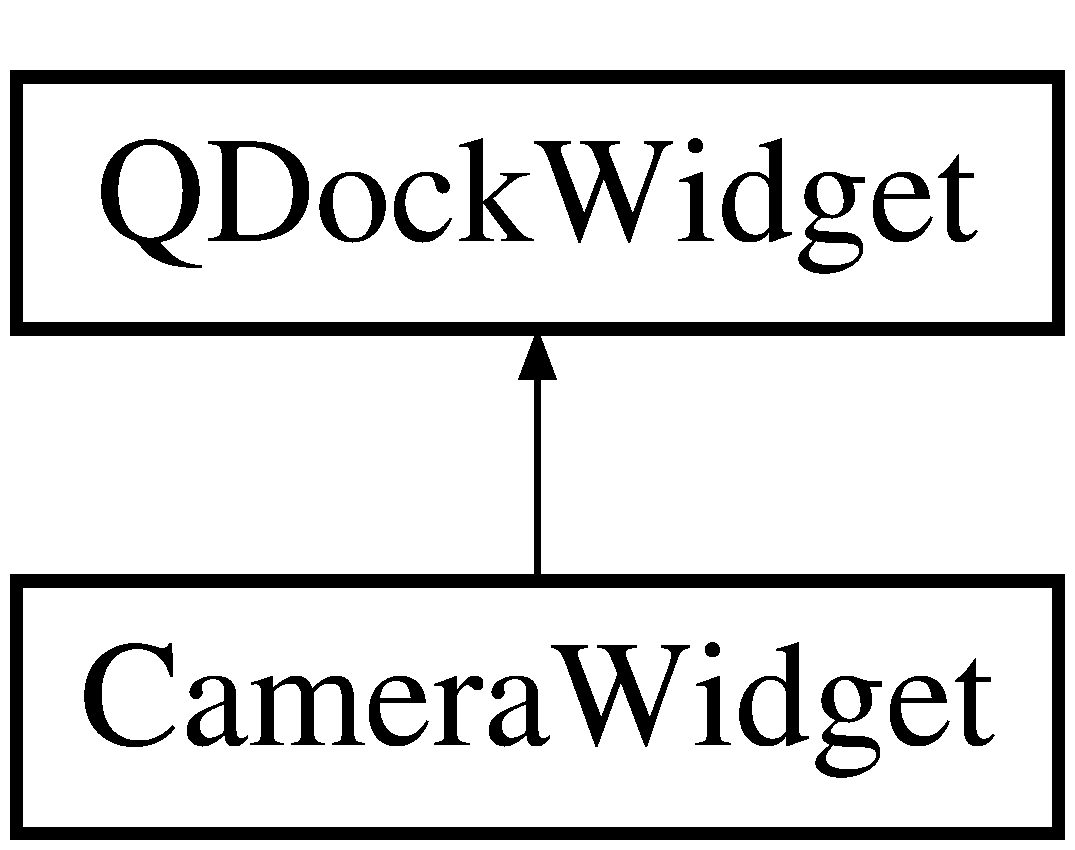
\includegraphics[height=2.000000cm]{classCameraWidget}
\end{center}
\end{figure}
\subsection*{Public Member Functions}
\begin{DoxyCompactItemize}
\item 
\hyperlink{classCameraWidget_a637ffd88fb213dad01dfa7294248029e}{Camera\-Widget} (Q\-Widget $\ast$parent=0)
\end{DoxyCompactItemize}
\subsection*{Private Attributes}
\begin{DoxyCompactItemize}
\item 
Q\-Push\-Button $\ast$ \hyperlink{classCameraWidget_a543f4c84a21b9e5e8ee536632f0cff74}{start\-Button}
\item 
Q\-Push\-Button $\ast$ \hyperlink{classCameraWidget_a93e74216fec1ab83f8e05efa54b631a1}{stop\-Button}
\end{DoxyCompactItemize}


\subsection{Constructor \& Destructor Documentation}
\hypertarget{classCameraWidget_a637ffd88fb213dad01dfa7294248029e}{\index{Camera\-Widget@{Camera\-Widget}!Camera\-Widget@{Camera\-Widget}}
\index{Camera\-Widget@{Camera\-Widget}!CameraWidget@{Camera\-Widget}}
\subsubsection[{Camera\-Widget}]{\setlength{\rightskip}{0pt plus 5cm}Camera\-Widget\-::\-Camera\-Widget (
\begin{DoxyParamCaption}
\item[{Q\-Widget $\ast$}]{parent = {\ttfamily 0}}
\end{DoxyParamCaption}
)\hspace{0.3cm}{\ttfamily [explicit]}}}\label{classCameraWidget_a637ffd88fb213dad01dfa7294248029e}


\subsection{Member Data Documentation}
\hypertarget{classCameraWidget_a543f4c84a21b9e5e8ee536632f0cff74}{\index{Camera\-Widget@{Camera\-Widget}!start\-Button@{start\-Button}}
\index{start\-Button@{start\-Button}!CameraWidget@{Camera\-Widget}}
\subsubsection[{start\-Button}]{\setlength{\rightskip}{0pt plus 5cm}Q\-Push\-Button$\ast$ Camera\-Widget\-::start\-Button\hspace{0.3cm}{\ttfamily [private]}}}\label{classCameraWidget_a543f4c84a21b9e5e8ee536632f0cff74}
\hypertarget{classCameraWidget_a93e74216fec1ab83f8e05efa54b631a1}{\index{Camera\-Widget@{Camera\-Widget}!stop\-Button@{stop\-Button}}
\index{stop\-Button@{stop\-Button}!CameraWidget@{Camera\-Widget}}
\subsubsection[{stop\-Button}]{\setlength{\rightskip}{0pt plus 5cm}Q\-Push\-Button$\ast$ Camera\-Widget\-::stop\-Button\hspace{0.3cm}{\ttfamily [private]}}}\label{classCameraWidget_a93e74216fec1ab83f8e05efa54b631a1}


The documentation for this class was generated from the following files\-:\begin{DoxyCompactItemize}
\item 
Base\-Station/\-Payload\-G\-U\-I/\hyperlink{CameraWidget_8h}{Camera\-Widget.\-h}\item 
Base\-Station/\-Payload\-G\-U\-I/\hyperlink{CameraWidget_8cpp}{Camera\-Widget.\-cpp}\end{DoxyCompactItemize}

\hypertarget{structDDMParams}{\section{D\-D\-M\-Params Struct Reference}
\label{structDDMParams}\index{D\-D\-M\-Params@{D\-D\-M\-Params}}
}
\subsection*{Public Member Functions}
\begin{DoxyCompactItemize}
\item 
\hyperlink{structDDMParams_a32113468489a6bf149e967f1b62da042}{D\-D\-M\-Params} ()
\item 
\hyperlink{structDDMParams_a01e60a17b71a55ef052ceba97d9a370f}{D\-D\-M\-Params} (const string \-\_\-detector\-Type, const string \-\_\-descriptor\-Type, const string \&\-\_\-matcher\-Type)
\item 
void \hyperlink{structDDMParams_a13b08a3275f499f7f54efc6f61dbbf2e}{read} (const File\-Node \&fn)
\item 
void \hyperlink{structDDMParams_ab224e3aa884d7af5a95af51caa0a290a}{write} (File\-Storage \&fs) const 
\item 
void \hyperlink{structDDMParams_af49a52d391d8fe0d27942d47f46bc2d9}{print} () const 
\end{DoxyCompactItemize}
\subsection*{Public Attributes}
\begin{DoxyCompactItemize}
\item 
string \hyperlink{structDDMParams_a7a13119000263119c574f88b11f3f9a6}{detector\-Type}
\item 
string \hyperlink{structDDMParams_acd9a38edfafc783a97a4ede7337b48d7}{descriptor\-Type}
\item 
string \hyperlink{structDDMParams_abc008f2603cebb2aff44945b0a4f66a5}{matcher\-Type}
\end{DoxyCompactItemize}


\subsection{Constructor \& Destructor Documentation}
\hypertarget{structDDMParams_a32113468489a6bf149e967f1b62da042}{\index{D\-D\-M\-Params@{D\-D\-M\-Params}!D\-D\-M\-Params@{D\-D\-M\-Params}}
\index{D\-D\-M\-Params@{D\-D\-M\-Params}!DDMParams@{D\-D\-M\-Params}}
\subsubsection[{D\-D\-M\-Params}]{\setlength{\rightskip}{0pt plus 5cm}D\-D\-M\-Params\-::\-D\-D\-M\-Params (
\begin{DoxyParamCaption}
{}
\end{DoxyParamCaption}
)\hspace{0.3cm}{\ttfamily [inline]}}}\label{structDDMParams_a32113468489a6bf149e967f1b62da042}
\hypertarget{structDDMParams_a01e60a17b71a55ef052ceba97d9a370f}{\index{D\-D\-M\-Params@{D\-D\-M\-Params}!D\-D\-M\-Params@{D\-D\-M\-Params}}
\index{D\-D\-M\-Params@{D\-D\-M\-Params}!DDMParams@{D\-D\-M\-Params}}
\subsubsection[{D\-D\-M\-Params}]{\setlength{\rightskip}{0pt plus 5cm}D\-D\-M\-Params\-::\-D\-D\-M\-Params (
\begin{DoxyParamCaption}
\item[{const string}]{\-\_\-detector\-Type, }
\item[{const string}]{\-\_\-descriptor\-Type, }
\item[{const string \&}]{\-\_\-matcher\-Type}
\end{DoxyParamCaption}
)\hspace{0.3cm}{\ttfamily [inline]}}}\label{structDDMParams_a01e60a17b71a55ef052ceba97d9a370f}


\subsection{Member Function Documentation}
\hypertarget{structDDMParams_af49a52d391d8fe0d27942d47f46bc2d9}{\index{D\-D\-M\-Params@{D\-D\-M\-Params}!print@{print}}
\index{print@{print}!DDMParams@{D\-D\-M\-Params}}
\subsubsection[{print}]{\setlength{\rightskip}{0pt plus 5cm}void D\-D\-M\-Params\-::print (
\begin{DoxyParamCaption}
{}
\end{DoxyParamCaption}
) const\hspace{0.3cm}{\ttfamily [inline]}}}\label{structDDMParams_af49a52d391d8fe0d27942d47f46bc2d9}
\hypertarget{structDDMParams_a13b08a3275f499f7f54efc6f61dbbf2e}{\index{D\-D\-M\-Params@{D\-D\-M\-Params}!read@{read}}
\index{read@{read}!DDMParams@{D\-D\-M\-Params}}
\subsubsection[{read}]{\setlength{\rightskip}{0pt plus 5cm}void D\-D\-M\-Params\-::read (
\begin{DoxyParamCaption}
\item[{const File\-Node \&}]{fn}
\end{DoxyParamCaption}
)\hspace{0.3cm}{\ttfamily [inline]}}}\label{structDDMParams_a13b08a3275f499f7f54efc6f61dbbf2e}
\hypertarget{structDDMParams_ab224e3aa884d7af5a95af51caa0a290a}{\index{D\-D\-M\-Params@{D\-D\-M\-Params}!write@{write}}
\index{write@{write}!DDMParams@{D\-D\-M\-Params}}
\subsubsection[{write}]{\setlength{\rightskip}{0pt plus 5cm}void D\-D\-M\-Params\-::write (
\begin{DoxyParamCaption}
\item[{File\-Storage \&}]{fs}
\end{DoxyParamCaption}
) const\hspace{0.3cm}{\ttfamily [inline]}}}\label{structDDMParams_ab224e3aa884d7af5a95af51caa0a290a}


\subsection{Member Data Documentation}
\hypertarget{structDDMParams_acd9a38edfafc783a97a4ede7337b48d7}{\index{D\-D\-M\-Params@{D\-D\-M\-Params}!descriptor\-Type@{descriptor\-Type}}
\index{descriptor\-Type@{descriptor\-Type}!DDMParams@{D\-D\-M\-Params}}
\subsubsection[{descriptor\-Type}]{\setlength{\rightskip}{0pt plus 5cm}string D\-D\-M\-Params\-::descriptor\-Type}}\label{structDDMParams_acd9a38edfafc783a97a4ede7337b48d7}
\hypertarget{structDDMParams_a7a13119000263119c574f88b11f3f9a6}{\index{D\-D\-M\-Params@{D\-D\-M\-Params}!detector\-Type@{detector\-Type}}
\index{detector\-Type@{detector\-Type}!DDMParams@{D\-D\-M\-Params}}
\subsubsection[{detector\-Type}]{\setlength{\rightskip}{0pt plus 5cm}string D\-D\-M\-Params\-::detector\-Type}}\label{structDDMParams_a7a13119000263119c574f88b11f3f9a6}
\hypertarget{structDDMParams_abc008f2603cebb2aff44945b0a4f66a5}{\index{D\-D\-M\-Params@{D\-D\-M\-Params}!matcher\-Type@{matcher\-Type}}
\index{matcher\-Type@{matcher\-Type}!DDMParams@{D\-D\-M\-Params}}
\subsubsection[{matcher\-Type}]{\setlength{\rightskip}{0pt plus 5cm}string D\-D\-M\-Params\-::matcher\-Type}}\label{structDDMParams_abc008f2603cebb2aff44945b0a4f66a5}


The documentation for this struct was generated from the following file\-:\begin{DoxyCompactItemize}
\item 
Payload/\-A\-D\-L\-C/\-Shape\-Characterization/\-Open\-C\-V\-Example/\hyperlink{bagofwords__classification_8cpp}{bagofwords\-\_\-classification.\-cpp}\end{DoxyCompactItemize}

\hypertarget{classDimage}{\section{Dimage Class Reference}
\label{classDimage}\index{Dimage@{Dimage}}
}


{\ttfamily \#include $<$Dimage.\-h$>$}

\subsection*{Public Member Functions}
\begin{DoxyCompactItemize}
\item 
\hyperlink{classDimage_a7f9e6f11d276696ece0e965bf7b49a59}{Dimage} ()
\item 
\hyperlink{classDimage_a5e4573b7b090d1a4da4c8782f78d91f7}{Dimage} (char $\ast$image\-Path)
\item 
bool \hyperlink{classDimage_ac6b561cd3c19c9ec5947932a3ad0e2fb}{has\-Target} ()
\item 
void \hyperlink{classDimage_a5a7fb91f2c4781473f71e3da828c1015}{salient\-\_\-detection} ()
\item 
void \hyperlink{classDimage_ab8edde46632c1ef26cd7b85357fb9e88}{Shape\-Detection} ()
\item 
void \hyperlink{classDimage_ab4ed2ec1c9edca1ae07459aaa46e440b}{Letter\-Detection} ()
\item 
void \hyperlink{classDimage_a0340c98df1a38d7026fa3816e0f78e90}{Color\-Detection} ()
\item 
void \hyperlink{classDimage_a49206c6028e3121d4cc320a835fa702b}{Tag} ()
\item 
\hyperlink{classDimage_a7f9e6f11d276696ece0e965bf7b49a59}{Dimage} ()
\item 
\hyperlink{classDimage_a5e4573b7b090d1a4da4c8782f78d91f7}{Dimage} (char $\ast$image\-Path)
\item 
bool \hyperlink{classDimage_ac6b561cd3c19c9ec5947932a3ad0e2fb}{has\-Target} ()
\item 
void \hyperlink{classDimage_a7e0080a7a776f312698e7112fd827dd0}{Salient} ()
\item 
void \hyperlink{classDimage_ab8edde46632c1ef26cd7b85357fb9e88}{Shape\-Detection} ()
\item 
void \hyperlink{classDimage_ab4ed2ec1c9edca1ae07459aaa46e440b}{Letter\-Detection} ()
\item 
void \hyperlink{classDimage_a0340c98df1a38d7026fa3816e0f78e90}{Color\-Detection} ()
\item 
void \hyperlink{classDimage_a49206c6028e3121d4cc320a835fa702b}{Tag} ()
\end{DoxyCompactItemize}
\subsection*{Public Attributes}
\begin{DoxyCompactItemize}
\item 
bool \hyperlink{classDimage_aa0e2203121319a2f3d5461a8ec161694}{target\-\_\-flag}
\item 
int \hyperlink{classDimage_ad9ebd4c340098de74c0971be6161f194}{altitude}
\item 
int \hyperlink{classDimage_a518750ead775e0dc036fe5885069dbf2}{latitude}
\item 
int \hyperlink{classDimage_abf468948c7b45b33fe37e653ca96c33d}{longitude}
\item 
float \hyperlink{classDimage_a6d13db78abfb30ba2829badef047a632}{degrees}
\item 
vector$<$ Rect $>$ \hyperlink{classDimage_a84e08d484952cbe4f1375826924f1ee9}{R\-O\-I}
\item 
vector$<$ \hyperlink{structTarget}{Target} $>$ \hyperlink{classDimage_a63f52e6d093db216a710643fb9852af0}{objects}
\item 
Mat \hyperlink{classDimage_a0da4164eece652cf86fc8ec27e2df086}{image}
\end{DoxyCompactItemize}


\subsection{Constructor \& Destructor Documentation}
\hypertarget{classDimage_a7f9e6f11d276696ece0e965bf7b49a59}{\index{Dimage@{Dimage}!Dimage@{Dimage}}
\index{Dimage@{Dimage}!Dimage@{Dimage}}
\subsubsection[{Dimage}]{\setlength{\rightskip}{0pt plus 5cm}Dimage\-::\-Dimage (
\begin{DoxyParamCaption}
{}
\end{DoxyParamCaption}
)}}\label{classDimage_a7f9e6f11d276696ece0e965bf7b49a59}
\hypertarget{classDimage_a5e4573b7b090d1a4da4c8782f78d91f7}{\index{Dimage@{Dimage}!Dimage@{Dimage}}
\index{Dimage@{Dimage}!Dimage@{Dimage}}
\subsubsection[{Dimage}]{\setlength{\rightskip}{0pt plus 5cm}Dimage\-::\-Dimage (
\begin{DoxyParamCaption}
\item[{char $\ast$}]{image\-Path}
\end{DoxyParamCaption}
)}}\label{classDimage_a5e4573b7b090d1a4da4c8782f78d91f7}
\hypertarget{classDimage_a7f9e6f11d276696ece0e965bf7b49a59}{\index{Dimage@{Dimage}!Dimage@{Dimage}}
\index{Dimage@{Dimage}!Dimage@{Dimage}}
\subsubsection[{Dimage}]{\setlength{\rightskip}{0pt plus 5cm}Dimage\-::\-Dimage (
\begin{DoxyParamCaption}
{}
\end{DoxyParamCaption}
)}}\label{classDimage_a7f9e6f11d276696ece0e965bf7b49a59}
\hypertarget{classDimage_a5e4573b7b090d1a4da4c8782f78d91f7}{\index{Dimage@{Dimage}!Dimage@{Dimage}}
\index{Dimage@{Dimage}!Dimage@{Dimage}}
\subsubsection[{Dimage}]{\setlength{\rightskip}{0pt plus 5cm}Dimage\-::\-Dimage (
\begin{DoxyParamCaption}
\item[{char $\ast$}]{image\-Path}
\end{DoxyParamCaption}
)}}\label{classDimage_a5e4573b7b090d1a4da4c8782f78d91f7}


\subsection{Member Function Documentation}
\hypertarget{classDimage_a0340c98df1a38d7026fa3816e0f78e90}{\index{Dimage@{Dimage}!Color\-Detection@{Color\-Detection}}
\index{Color\-Detection@{Color\-Detection}!Dimage@{Dimage}}
\subsubsection[{Color\-Detection}]{\setlength{\rightskip}{0pt plus 5cm}void Dimage\-::\-Color\-Detection (
\begin{DoxyParamCaption}
{}
\end{DoxyParamCaption}
)}}\label{classDimage_a0340c98df1a38d7026fa3816e0f78e90}
\hypertarget{classDimage_a0340c98df1a38d7026fa3816e0f78e90}{\index{Dimage@{Dimage}!Color\-Detection@{Color\-Detection}}
\index{Color\-Detection@{Color\-Detection}!Dimage@{Dimage}}
\subsubsection[{Color\-Detection}]{\setlength{\rightskip}{0pt plus 5cm}void Dimage\-::\-Color\-Detection (
\begin{DoxyParamCaption}
{}
\end{DoxyParamCaption}
)}}\label{classDimage_a0340c98df1a38d7026fa3816e0f78e90}
\hypertarget{classDimage_ac6b561cd3c19c9ec5947932a3ad0e2fb}{\index{Dimage@{Dimage}!has\-Target@{has\-Target}}
\index{has\-Target@{has\-Target}!Dimage@{Dimage}}
\subsubsection[{has\-Target}]{\setlength{\rightskip}{0pt plus 5cm}bool Dimage\-::has\-Target (
\begin{DoxyParamCaption}
{}
\end{DoxyParamCaption}
)}}\label{classDimage_ac6b561cd3c19c9ec5947932a3ad0e2fb}
\hypertarget{classDimage_ac6b561cd3c19c9ec5947932a3ad0e2fb}{\index{Dimage@{Dimage}!has\-Target@{has\-Target}}
\index{has\-Target@{has\-Target}!Dimage@{Dimage}}
\subsubsection[{has\-Target}]{\setlength{\rightskip}{0pt plus 5cm}bool Dimage\-::has\-Target (
\begin{DoxyParamCaption}
{}
\end{DoxyParamCaption}
)}}\label{classDimage_ac6b561cd3c19c9ec5947932a3ad0e2fb}
\hypertarget{classDimage_ab4ed2ec1c9edca1ae07459aaa46e440b}{\index{Dimage@{Dimage}!Letter\-Detection@{Letter\-Detection}}
\index{Letter\-Detection@{Letter\-Detection}!Dimage@{Dimage}}
\subsubsection[{Letter\-Detection}]{\setlength{\rightskip}{0pt plus 5cm}void Dimage\-::\-Letter\-Detection (
\begin{DoxyParamCaption}
{}
\end{DoxyParamCaption}
)}}\label{classDimage_ab4ed2ec1c9edca1ae07459aaa46e440b}
\hypertarget{classDimage_ab4ed2ec1c9edca1ae07459aaa46e440b}{\index{Dimage@{Dimage}!Letter\-Detection@{Letter\-Detection}}
\index{Letter\-Detection@{Letter\-Detection}!Dimage@{Dimage}}
\subsubsection[{Letter\-Detection}]{\setlength{\rightskip}{0pt plus 5cm}void Dimage\-::\-Letter\-Detection (
\begin{DoxyParamCaption}
{}
\end{DoxyParamCaption}
)}}\label{classDimage_ab4ed2ec1c9edca1ae07459aaa46e440b}
\hypertarget{classDimage_a7e0080a7a776f312698e7112fd827dd0}{\index{Dimage@{Dimage}!Salient@{Salient}}
\index{Salient@{Salient}!Dimage@{Dimage}}
\subsubsection[{Salient}]{\setlength{\rightskip}{0pt plus 5cm}void Dimage\-::\-Salient (
\begin{DoxyParamCaption}
{}
\end{DoxyParamCaption}
)}}\label{classDimage_a7e0080a7a776f312698e7112fd827dd0}
\hypertarget{classDimage_a5a7fb91f2c4781473f71e3da828c1015}{\index{Dimage@{Dimage}!salient\-\_\-detection@{salient\-\_\-detection}}
\index{salient\-\_\-detection@{salient\-\_\-detection}!Dimage@{Dimage}}
\subsubsection[{salient\-\_\-detection}]{\setlength{\rightskip}{0pt plus 5cm}void Dimage\-::salient\-\_\-detection (
\begin{DoxyParamCaption}
{}
\end{DoxyParamCaption}
)}}\label{classDimage_a5a7fb91f2c4781473f71e3da828c1015}
Find contours

Approximate contours to polygons + get bounding rects and circles \hypertarget{classDimage_ab8edde46632c1ef26cd7b85357fb9e88}{\index{Dimage@{Dimage}!Shape\-Detection@{Shape\-Detection}}
\index{Shape\-Detection@{Shape\-Detection}!Dimage@{Dimage}}
\subsubsection[{Shape\-Detection}]{\setlength{\rightskip}{0pt plus 5cm}void Dimage\-::\-Shape\-Detection (
\begin{DoxyParamCaption}
{}
\end{DoxyParamCaption}
)}}\label{classDimage_ab8edde46632c1ef26cd7b85357fb9e88}
\hypertarget{classDimage_ab8edde46632c1ef26cd7b85357fb9e88}{\index{Dimage@{Dimage}!Shape\-Detection@{Shape\-Detection}}
\index{Shape\-Detection@{Shape\-Detection}!Dimage@{Dimage}}
\subsubsection[{Shape\-Detection}]{\setlength{\rightskip}{0pt plus 5cm}void Dimage\-::\-Shape\-Detection (
\begin{DoxyParamCaption}
{}
\end{DoxyParamCaption}
)}}\label{classDimage_ab8edde46632c1ef26cd7b85357fb9e88}
\hypertarget{classDimage_a49206c6028e3121d4cc320a835fa702b}{\index{Dimage@{Dimage}!Tag@{Tag}}
\index{Tag@{Tag}!Dimage@{Dimage}}
\subsubsection[{Tag}]{\setlength{\rightskip}{0pt plus 5cm}void Dimage\-::\-Tag (
\begin{DoxyParamCaption}
{}
\end{DoxyParamCaption}
)}}\label{classDimage_a49206c6028e3121d4cc320a835fa702b}
\hypertarget{classDimage_a49206c6028e3121d4cc320a835fa702b}{\index{Dimage@{Dimage}!Tag@{Tag}}
\index{Tag@{Tag}!Dimage@{Dimage}}
\subsubsection[{Tag}]{\setlength{\rightskip}{0pt plus 5cm}void Dimage\-::\-Tag (
\begin{DoxyParamCaption}
{}
\end{DoxyParamCaption}
)}}\label{classDimage_a49206c6028e3121d4cc320a835fa702b}


\subsection{Member Data Documentation}
\hypertarget{classDimage_ad9ebd4c340098de74c0971be6161f194}{\index{Dimage@{Dimage}!altitude@{altitude}}
\index{altitude@{altitude}!Dimage@{Dimage}}
\subsubsection[{altitude}]{\setlength{\rightskip}{0pt plus 5cm}int Dimage\-::altitude}}\label{classDimage_ad9ebd4c340098de74c0971be6161f194}
\hypertarget{classDimage_a6d13db78abfb30ba2829badef047a632}{\index{Dimage@{Dimage}!degrees@{degrees}}
\index{degrees@{degrees}!Dimage@{Dimage}}
\subsubsection[{degrees}]{\setlength{\rightskip}{0pt plus 5cm}float Dimage\-::degrees}}\label{classDimage_a6d13db78abfb30ba2829badef047a632}
\hypertarget{classDimage_a0da4164eece652cf86fc8ec27e2df086}{\index{Dimage@{Dimage}!image@{image}}
\index{image@{image}!Dimage@{Dimage}}
\subsubsection[{image}]{\setlength{\rightskip}{0pt plus 5cm}Mat Dimage\-::image}}\label{classDimage_a0da4164eece652cf86fc8ec27e2df086}
\hypertarget{classDimage_a518750ead775e0dc036fe5885069dbf2}{\index{Dimage@{Dimage}!latitude@{latitude}}
\index{latitude@{latitude}!Dimage@{Dimage}}
\subsubsection[{latitude}]{\setlength{\rightskip}{0pt plus 5cm}int Dimage\-::latitude}}\label{classDimage_a518750ead775e0dc036fe5885069dbf2}
\hypertarget{classDimage_abf468948c7b45b33fe37e653ca96c33d}{\index{Dimage@{Dimage}!longitude@{longitude}}
\index{longitude@{longitude}!Dimage@{Dimage}}
\subsubsection[{longitude}]{\setlength{\rightskip}{0pt plus 5cm}int Dimage\-::longitude}}\label{classDimage_abf468948c7b45b33fe37e653ca96c33d}
\hypertarget{classDimage_a63f52e6d093db216a710643fb9852af0}{\index{Dimage@{Dimage}!objects@{objects}}
\index{objects@{objects}!Dimage@{Dimage}}
\subsubsection[{objects}]{\setlength{\rightskip}{0pt plus 5cm}vector$<$ {\bf Target} $>$ Dimage\-::objects}}\label{classDimage_a63f52e6d093db216a710643fb9852af0}
\hypertarget{classDimage_a84e08d484952cbe4f1375826924f1ee9}{\index{Dimage@{Dimage}!R\-O\-I@{R\-O\-I}}
\index{R\-O\-I@{R\-O\-I}!Dimage@{Dimage}}
\subsubsection[{R\-O\-I}]{\setlength{\rightskip}{0pt plus 5cm}vector$<$ Rect $>$ Dimage\-::\-R\-O\-I}}\label{classDimage_a84e08d484952cbe4f1375826924f1ee9}
\hypertarget{classDimage_aa0e2203121319a2f3d5461a8ec161694}{\index{Dimage@{Dimage}!target\-\_\-flag@{target\-\_\-flag}}
\index{target\-\_\-flag@{target\-\_\-flag}!Dimage@{Dimage}}
\subsubsection[{target\-\_\-flag}]{\setlength{\rightskip}{0pt plus 5cm}bool Dimage\-::target\-\_\-flag}}\label{classDimage_aa0e2203121319a2f3d5461a8ec161694}


The documentation for this class was generated from the following files\-:\begin{DoxyCompactItemize}
\item 
Base\-Station/\-A\-D\-L\-C/inc/\hyperlink{BaseStation_2ADLC_2inc_2Dimage_8h}{Dimage.\-h}\item 
Base\-Station/\-A\-D\-L\-C/src/\hyperlink{Dimage_8cpp}{Dimage.\-cpp}\item 
Base\-Station/\-A\-D\-L\-C/src/\hyperlink{Salient_8cpp}{Salient.\-cpp}\end{DoxyCompactItemize}

\hypertarget{classMainWindow}{\section{Main\-Window Class Reference}
\label{classMainWindow}\index{Main\-Window@{Main\-Window}}
}


The main window for this application.  




{\ttfamily \#include $<$Main\-Window.\-h$>$}

Inheritance diagram for Main\-Window\-:\begin{figure}[H]
\begin{center}
\leavevmode
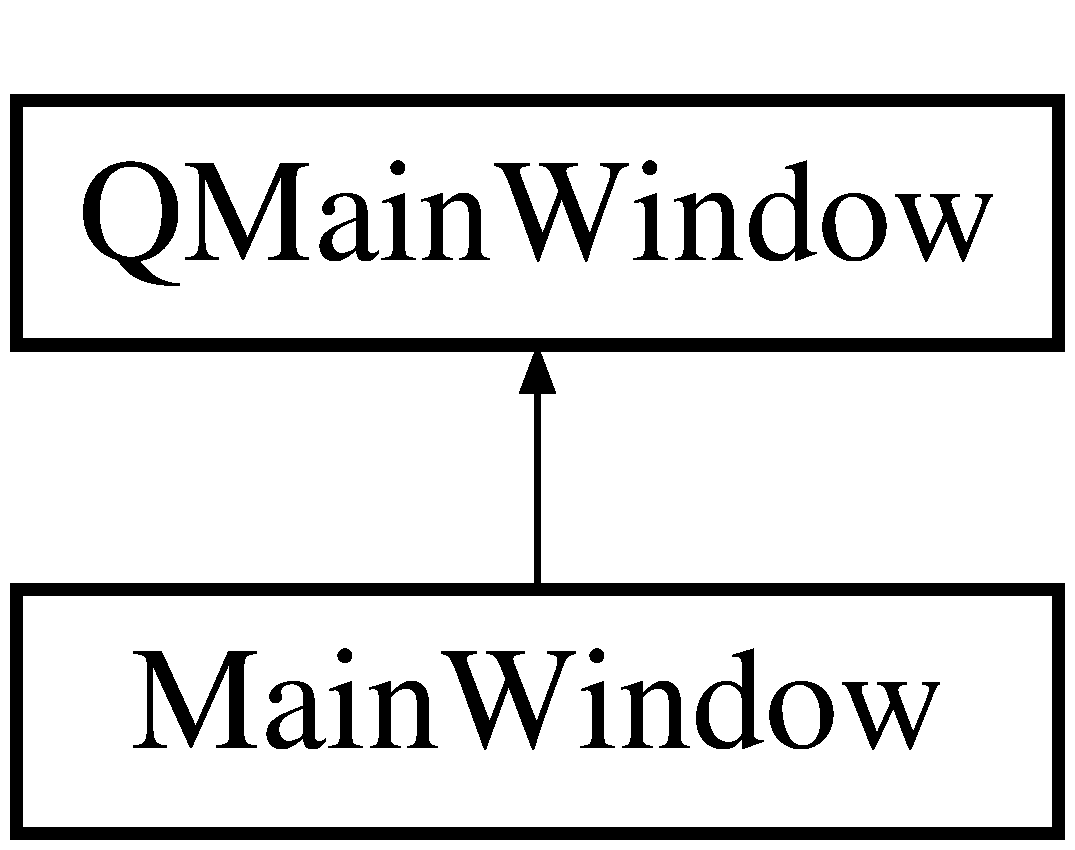
\includegraphics[height=2.000000cm]{classMainWindow}
\end{center}
\end{figure}
\subsection*{Public Member Functions}
\begin{DoxyCompactItemize}
\item 
\hyperlink{classMainWindow_ab7d94977fe4f15c9850f3e4928e02672}{Main\-Window} (Q\-Main\-Window $\ast$parent=0)
\end{DoxyCompactItemize}
\subsection*{Private Attributes}
\begin{DoxyCompactItemize}
\item 
\hyperlink{classNetworkWidget}{Network\-Widget} $\ast$ \hyperlink{classMainWindow_a28553a574d726f7be2831c6d4590096b}{Network}
\begin{DoxyCompactList}\small\item\em The widget that controlls the network. \end{DoxyCompactList}\item 
\hyperlink{classCameraWidget}{Camera\-Widget} $\ast$ \hyperlink{classMainWindow_a941b44f2384c25f45dbba74c4dc3dd7d}{Camera}
\begin{DoxyCompactList}\small\item\em The widget that controlls the camera. \end{DoxyCompactList}\end{DoxyCompactItemize}


\subsection{Detailed Description}
The main window for this application. 

This \hyperlink{classMainWindow}{Main\-Window} class inherits from Q\-Main\-Window and is the primary application window in which all other widgets dock into. 

\subsection{Constructor \& Destructor Documentation}
\hypertarget{classMainWindow_ab7d94977fe4f15c9850f3e4928e02672}{\index{Main\-Window@{Main\-Window}!Main\-Window@{Main\-Window}}
\index{Main\-Window@{Main\-Window}!MainWindow@{Main\-Window}}
\subsubsection[{Main\-Window}]{\setlength{\rightskip}{0pt plus 5cm}Main\-Window\-::\-Main\-Window (
\begin{DoxyParamCaption}
\item[{Q\-Main\-Window $\ast$}]{parent = {\ttfamily 0}}
\end{DoxyParamCaption}
)\hspace{0.3cm}{\ttfamily [explicit]}}}\label{classMainWindow_ab7d94977fe4f15c9850f3e4928e02672}


\subsection{Member Data Documentation}
\hypertarget{classMainWindow_a941b44f2384c25f45dbba74c4dc3dd7d}{\index{Main\-Window@{Main\-Window}!Camera@{Camera}}
\index{Camera@{Camera}!MainWindow@{Main\-Window}}
\subsubsection[{Camera}]{\setlength{\rightskip}{0pt plus 5cm}{\bf Camera\-Widget}$\ast$ Main\-Window\-::\-Camera\hspace{0.3cm}{\ttfamily [private]}}}\label{classMainWindow_a941b44f2384c25f45dbba74c4dc3dd7d}


The widget that controlls the camera. 

\hypertarget{classMainWindow_a28553a574d726f7be2831c6d4590096b}{\index{Main\-Window@{Main\-Window}!Network@{Network}}
\index{Network@{Network}!MainWindow@{Main\-Window}}
\subsubsection[{Network}]{\setlength{\rightskip}{0pt plus 5cm}{\bf Network\-Widget}$\ast$ Main\-Window\-::\-Network\hspace{0.3cm}{\ttfamily [private]}}}\label{classMainWindow_a28553a574d726f7be2831c6d4590096b}


The widget that controlls the network. 



The documentation for this class was generated from the following files\-:\begin{DoxyCompactItemize}
\item 
Base\-Station/\-Payload\-G\-U\-I/\hyperlink{MainWindow_8h}{Main\-Window.\-h}\item 
Base\-Station/\-Payload\-G\-U\-I/\hyperlink{MainWindow_8cpp}{Main\-Window.\-cpp}\end{DoxyCompactItemize}

\hypertarget{classNetwork}{\section{Network Class Reference}
\label{classNetwork}\index{Network@{Network}}
}


{\ttfamily \#include $<$Network.\-h$>$}



The documentation for this class was generated from the following file\-:\begin{DoxyCompactItemize}
\item 
Base\-Station/\-Base\-Station\-Comms/\hyperlink{Network_8h}{Network.\-h}\end{DoxyCompactItemize}

\hypertarget{classNetworkWidget}{\section{Network\-Widget Class Reference}
\label{classNetworkWidget}\index{Network\-Widget@{Network\-Widget}}
}


{\ttfamily \#include $<$Network\-Widget.\-h$>$}

Inheritance diagram for Network\-Widget\-:\begin{figure}[H]
\begin{center}
\leavevmode
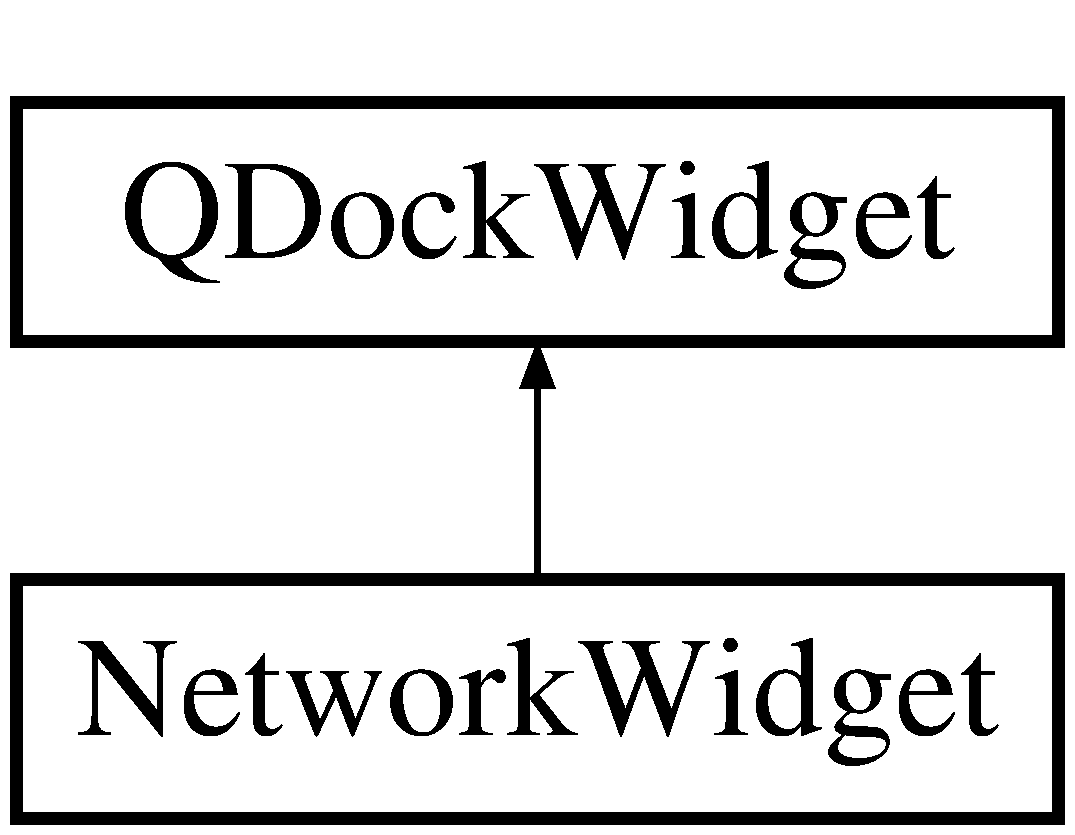
\includegraphics[height=2.000000cm]{classNetworkWidget}
\end{center}
\end{figure}
\subsection*{Public Member Functions}
\begin{DoxyCompactItemize}
\item 
\hyperlink{classNetworkWidget_ad83b8a39a5ca607c6276ddd3c250f9f7}{Network\-Widget} (Q\-Widget $\ast$parent=0)
\end{DoxyCompactItemize}
\subsection*{Private Attributes}
\begin{DoxyCompactItemize}
\item 
Q\-Push\-Button $\ast$ \hyperlink{classNetworkWidget_a310960ed56867e9dfe77f41652c70e86}{start\-Button}
\item 
Q\-Push\-Button $\ast$ \hyperlink{classNetworkWidget_abd91e508b53a4a911eb482a5ea36fd51}{stop\-Button}
\end{DoxyCompactItemize}


\subsection{Constructor \& Destructor Documentation}
\hypertarget{classNetworkWidget_ad83b8a39a5ca607c6276ddd3c250f9f7}{\index{Network\-Widget@{Network\-Widget}!Network\-Widget@{Network\-Widget}}
\index{Network\-Widget@{Network\-Widget}!NetworkWidget@{Network\-Widget}}
\subsubsection[{Network\-Widget}]{\setlength{\rightskip}{0pt plus 5cm}Network\-Widget\-::\-Network\-Widget (
\begin{DoxyParamCaption}
\item[{Q\-Widget $\ast$}]{parent = {\ttfamily 0}}
\end{DoxyParamCaption}
)\hspace{0.3cm}{\ttfamily [explicit]}}}\label{classNetworkWidget_ad83b8a39a5ca607c6276ddd3c250f9f7}


\subsection{Member Data Documentation}
\hypertarget{classNetworkWidget_a310960ed56867e9dfe77f41652c70e86}{\index{Network\-Widget@{Network\-Widget}!start\-Button@{start\-Button}}
\index{start\-Button@{start\-Button}!NetworkWidget@{Network\-Widget}}
\subsubsection[{start\-Button}]{\setlength{\rightskip}{0pt plus 5cm}Q\-Push\-Button$\ast$ Network\-Widget\-::start\-Button\hspace{0.3cm}{\ttfamily [private]}}}\label{classNetworkWidget_a310960ed56867e9dfe77f41652c70e86}
\hypertarget{classNetworkWidget_abd91e508b53a4a911eb482a5ea36fd51}{\index{Network\-Widget@{Network\-Widget}!stop\-Button@{stop\-Button}}
\index{stop\-Button@{stop\-Button}!NetworkWidget@{Network\-Widget}}
\subsubsection[{stop\-Button}]{\setlength{\rightskip}{0pt plus 5cm}Q\-Push\-Button$\ast$ Network\-Widget\-::stop\-Button\hspace{0.3cm}{\ttfamily [private]}}}\label{classNetworkWidget_abd91e508b53a4a911eb482a5ea36fd51}


The documentation for this class was generated from the following files\-:\begin{DoxyCompactItemize}
\item 
Base\-Station/\-Payload\-G\-U\-I/\hyperlink{NetworkWidget_8h}{Network\-Widget.\-h}\item 
Base\-Station/\-Payload\-G\-U\-I/\hyperlink{NetworkWidget_8cpp}{Network\-Widget.\-cpp}\end{DoxyCompactItemize}

\hypertarget{classObdImage}{\section{Obd\-Image Class Reference}
\label{classObdImage}\index{Obd\-Image@{Obd\-Image}}
}
\subsection*{Public Member Functions}
\begin{DoxyCompactItemize}
\item 
\hyperlink{classObdImage_a7b54069858f0de8578563a4e6557251d}{Obd\-Image} (string p\-\_\-id, string p\-\_\-path)
\end{DoxyCompactItemize}
\subsection*{Public Attributes}
\begin{DoxyCompactItemize}
\item 
string \hyperlink{classObdImage_ac2389a2b08a8607e2f553f17906d9eaa}{id}
\item 
string \hyperlink{classObdImage_a377e0798ce5595b84d1bd8f111628fca}{path}
\end{DoxyCompactItemize}


\subsection{Constructor \& Destructor Documentation}
\hypertarget{classObdImage_a7b54069858f0de8578563a4e6557251d}{\index{Obd\-Image@{Obd\-Image}!Obd\-Image@{Obd\-Image}}
\index{Obd\-Image@{Obd\-Image}!ObdImage@{Obd\-Image}}
\subsubsection[{Obd\-Image}]{\setlength{\rightskip}{0pt plus 5cm}Obd\-Image\-::\-Obd\-Image (
\begin{DoxyParamCaption}
\item[{string}]{p\-\_\-id, }
\item[{string}]{p\-\_\-path}
\end{DoxyParamCaption}
)\hspace{0.3cm}{\ttfamily [inline]}}}\label{classObdImage_a7b54069858f0de8578563a4e6557251d}


\subsection{Member Data Documentation}
\hypertarget{classObdImage_ac2389a2b08a8607e2f553f17906d9eaa}{\index{Obd\-Image@{Obd\-Image}!id@{id}}
\index{id@{id}!ObdImage@{Obd\-Image}}
\subsubsection[{id}]{\setlength{\rightskip}{0pt plus 5cm}string Obd\-Image\-::id}}\label{classObdImage_ac2389a2b08a8607e2f553f17906d9eaa}
\hypertarget{classObdImage_a377e0798ce5595b84d1bd8f111628fca}{\index{Obd\-Image@{Obd\-Image}!path@{path}}
\index{path@{path}!ObdImage@{Obd\-Image}}
\subsubsection[{path}]{\setlength{\rightskip}{0pt plus 5cm}string Obd\-Image\-::path}}\label{classObdImage_a377e0798ce5595b84d1bd8f111628fca}


The documentation for this class was generated from the following file\-:\begin{DoxyCompactItemize}
\item 
Payload/\-A\-D\-L\-C/\-Shape\-Characterization/\-Open\-C\-V\-Example/\hyperlink{bagofwords__classification_8cpp}{bagofwords\-\_\-classification.\-cpp}\end{DoxyCompactItemize}

\hypertarget{classObdObject}{\section{Obd\-Object Class Reference}
\label{classObdObject}\index{Obd\-Object@{Obd\-Object}}
}
\subsection*{Public Attributes}
\begin{DoxyCompactItemize}
\item 
string \hyperlink{classObdObject_ab40b6b9c31790ccd4da01a182802ab9c}{object\-\_\-class}
\item 
Rect \hyperlink{classObdObject_a06c5689641c3dc7f6e6ac3e2a28e2240}{bounding\-Box}
\end{DoxyCompactItemize}


\subsection{Member Data Documentation}
\hypertarget{classObdObject_a06c5689641c3dc7f6e6ac3e2a28e2240}{\index{Obd\-Object@{Obd\-Object}!bounding\-Box@{bounding\-Box}}
\index{bounding\-Box@{bounding\-Box}!ObdObject@{Obd\-Object}}
\subsubsection[{bounding\-Box}]{\setlength{\rightskip}{0pt plus 5cm}Rect Obd\-Object\-::bounding\-Box}}\label{classObdObject_a06c5689641c3dc7f6e6ac3e2a28e2240}
\hypertarget{classObdObject_ab40b6b9c31790ccd4da01a182802ab9c}{\index{Obd\-Object@{Obd\-Object}!object\-\_\-class@{object\-\_\-class}}
\index{object\-\_\-class@{object\-\_\-class}!ObdObject@{Obd\-Object}}
\subsubsection[{object\-\_\-class}]{\setlength{\rightskip}{0pt plus 5cm}string Obd\-Object\-::object\-\_\-class}}\label{classObdObject_ab40b6b9c31790ccd4da01a182802ab9c}


The documentation for this class was generated from the following file\-:\begin{DoxyCompactItemize}
\item 
Payload/\-A\-D\-L\-C/\-Shape\-Characterization/\-Open\-C\-V\-Example/\hyperlink{bagofwords__classification_8cpp}{bagofwords\-\_\-classification.\-cpp}\end{DoxyCompactItemize}

\hypertarget{classObdScoreIndexSorter}{\section{Obd\-Score\-Index\-Sorter Class Reference}
\label{classObdScoreIndexSorter}\index{Obd\-Score\-Index\-Sorter@{Obd\-Score\-Index\-Sorter}}
}
\subsection*{Public Member Functions}
\begin{DoxyCompactItemize}
\item 
bool \hyperlink{classObdScoreIndexSorter_a7d2a136be43f1ee843dfa81882ebaab2}{operator$<$} (const \hyperlink{classObdScoreIndexSorter}{Obd\-Score\-Index\-Sorter} \&compare) const 
\end{DoxyCompactItemize}
\subsection*{Public Attributes}
\begin{DoxyCompactItemize}
\item 
float \hyperlink{classObdScoreIndexSorter_a5c0adb2f526d018b41271e2898278fe7}{score}
\item 
int \hyperlink{classObdScoreIndexSorter_af88d59b2fcc6d307feca504bf6b5f532}{image\-\_\-idx}
\item 
int \hyperlink{classObdScoreIndexSorter_a691c567e854be72a33d81e3753fe1919}{obj\-\_\-idx}
\end{DoxyCompactItemize}


\subsection{Member Function Documentation}
\hypertarget{classObdScoreIndexSorter_a7d2a136be43f1ee843dfa81882ebaab2}{\index{Obd\-Score\-Index\-Sorter@{Obd\-Score\-Index\-Sorter}!operator$<$@{operator$<$}}
\index{operator$<$@{operator$<$}!ObdScoreIndexSorter@{Obd\-Score\-Index\-Sorter}}
\subsubsection[{operator$<$}]{\setlength{\rightskip}{0pt plus 5cm}bool Obd\-Score\-Index\-Sorter\-::operator$<$ (
\begin{DoxyParamCaption}
\item[{const {\bf Obd\-Score\-Index\-Sorter} \&}]{compare}
\end{DoxyParamCaption}
) const\hspace{0.3cm}{\ttfamily [inline]}}}\label{classObdScoreIndexSorter_a7d2a136be43f1ee843dfa81882ebaab2}


\subsection{Member Data Documentation}
\hypertarget{classObdScoreIndexSorter_af88d59b2fcc6d307feca504bf6b5f532}{\index{Obd\-Score\-Index\-Sorter@{Obd\-Score\-Index\-Sorter}!image\-\_\-idx@{image\-\_\-idx}}
\index{image\-\_\-idx@{image\-\_\-idx}!ObdScoreIndexSorter@{Obd\-Score\-Index\-Sorter}}
\subsubsection[{image\-\_\-idx}]{\setlength{\rightskip}{0pt plus 5cm}int Obd\-Score\-Index\-Sorter\-::image\-\_\-idx}}\label{classObdScoreIndexSorter_af88d59b2fcc6d307feca504bf6b5f532}
\hypertarget{classObdScoreIndexSorter_a691c567e854be72a33d81e3753fe1919}{\index{Obd\-Score\-Index\-Sorter@{Obd\-Score\-Index\-Sorter}!obj\-\_\-idx@{obj\-\_\-idx}}
\index{obj\-\_\-idx@{obj\-\_\-idx}!ObdScoreIndexSorter@{Obd\-Score\-Index\-Sorter}}
\subsubsection[{obj\-\_\-idx}]{\setlength{\rightskip}{0pt plus 5cm}int Obd\-Score\-Index\-Sorter\-::obj\-\_\-idx}}\label{classObdScoreIndexSorter_a691c567e854be72a33d81e3753fe1919}
\hypertarget{classObdScoreIndexSorter_a5c0adb2f526d018b41271e2898278fe7}{\index{Obd\-Score\-Index\-Sorter@{Obd\-Score\-Index\-Sorter}!score@{score}}
\index{score@{score}!ObdScoreIndexSorter@{Obd\-Score\-Index\-Sorter}}
\subsubsection[{score}]{\setlength{\rightskip}{0pt plus 5cm}float Obd\-Score\-Index\-Sorter\-::score}}\label{classObdScoreIndexSorter_a5c0adb2f526d018b41271e2898278fe7}


The documentation for this class was generated from the following file\-:\begin{DoxyCompactItemize}
\item 
Payload/\-A\-D\-L\-C/\-Shape\-Characterization/\-Open\-C\-V\-Example/\hyperlink{bagofwords__classification_8cpp}{bagofwords\-\_\-classification.\-cpp}\end{DoxyCompactItemize}

\hypertarget{structVocData_1_1orderingSorter}{\section{Voc\-Data\-:\-:ordering\-Sorter Struct Reference}
\label{structVocData_1_1orderingSorter}\index{Voc\-Data\-::ordering\-Sorter@{Voc\-Data\-::ordering\-Sorter}}
}
\subsection*{Public Member Functions}
\begin{DoxyCompactItemize}
\item 
bool \hyperlink{structVocData_1_1orderingSorter_ad23eb713639d9a29c1603cb22d41a9d3}{operator()} (std\-::pair$<$ size\-\_\-t, vector$<$ float $>$\-::const\-\_\-iterator $>$ const \&a, std\-::pair$<$ size\-\_\-t, vector$<$ float $>$\-::const\-\_\-iterator $>$ const \&b)
\end{DoxyCompactItemize}


\subsection{Member Function Documentation}
\hypertarget{structVocData_1_1orderingSorter_ad23eb713639d9a29c1603cb22d41a9d3}{\index{Voc\-Data\-::ordering\-Sorter@{Voc\-Data\-::ordering\-Sorter}!operator()@{operator()}}
\index{operator()@{operator()}!VocData::orderingSorter@{Voc\-Data\-::ordering\-Sorter}}
\subsubsection[{operator()}]{\setlength{\rightskip}{0pt plus 5cm}bool Voc\-Data\-::ordering\-Sorter\-::operator() (
\begin{DoxyParamCaption}
\item[{std\-::pair$<$ size\-\_\-t, vector$<$ float $>$\-::const\-\_\-iterator $>$ const \&}]{a, }
\item[{std\-::pair$<$ size\-\_\-t, vector$<$ float $>$\-::const\-\_\-iterator $>$ const \&}]{b}
\end{DoxyParamCaption}
)\hspace{0.3cm}{\ttfamily [inline]}}}\label{structVocData_1_1orderingSorter_ad23eb713639d9a29c1603cb22d41a9d3}


The documentation for this struct was generated from the following file\-:\begin{DoxyCompactItemize}
\item 
Payload/\-A\-D\-L\-C/\-Shape\-Characterization/\-Open\-C\-V\-Example/\hyperlink{bagofwords__classification_8cpp}{bagofwords\-\_\-classification.\-cpp}\end{DoxyCompactItemize}

\hypertarget{classPacketFramer}{\section{Packet\-Framer Class Reference}
\label{classPacketFramer}\index{Packet\-Framer@{Packet\-Framer}}
}


{\ttfamily \#include $<$Packet\-Framer.\-h$>$}



The documentation for this class was generated from the following file\-:\begin{DoxyCompactItemize}
\item 
Base\-Station/\-Base\-Station\-Comms/\hyperlink{PacketFramer_8h}{Packet\-Framer.\-h}\end{DoxyCompactItemize}

\hypertarget{classPacketMonitor}{\section{Packet\-Monitor Class Reference}
\label{classPacketMonitor}\index{Packet\-Monitor@{Packet\-Monitor}}
}


{\ttfamily \#include $<$Packet\-Monitor.\-h$>$}



The documentation for this class was generated from the following file\-:\begin{DoxyCompactItemize}
\item 
Base\-Station/\-Base\-Station\-Comms/\hyperlink{PacketMonitor_8h}{Packet\-Monitor.\-h}\end{DoxyCompactItemize}

\hypertarget{classPayloadStatus}{\section{Payload\-Status Class Reference}
\label{classPayloadStatus}\index{Payload\-Status@{Payload\-Status}}
}


{\ttfamily \#include $<$Payload\-Status.\-h$>$}



The documentation for this class was generated from the following file\-:\begin{DoxyCompactItemize}
\item 
Resources/\hyperlink{PayloadStatus_8h}{Payload\-Status.\-h}\end{DoxyCompactItemize}

\hypertarget{classSalient}{\section{Salient Class Reference}
\label{classSalient}\index{Salient@{Salient}}
}


{\ttfamily \#include $<$Salient.\-h$>$}

\subsection*{Public Member Functions}
\begin{DoxyCompactItemize}
\item 
\hyperlink{classSalient_ab833adc762328e9747ca67ec17bf61d2}{Salient} ()
\item 
\hyperlink{classSalient_a18d6eee5f1853e35bd6606f304dc2e97}{Salient} (Mat image)
\item 
\hyperlink{classSalient_a208b6601a6dbf6829cfc90999251e21f}{Salient} (Mat image, vector$<$ Rect $>$) Mat \hyperlink{SVM__detection_8cpp_a1a2bec3cfc31133af2c33d80d7a677a9}{salient\-\_\-detection}(Mat img)
\item 
Mat \hyperlink{classSalient_a0795ed8abaad113be8c42cf840b25cd2}{Canny\-Threshold} (Mat src, Mat grad)
\item 
Mat \hyperlink{classSalient_a048dcc50160b175791c55d794916c02a}{gradient} (Mat src)
\item 
void \hyperlink{classSalient_ab696dcd90383ffc4965b9be7c8d0d204}{find\-Object} (Mat mask, Mat src)
\end{DoxyCompactItemize}


\subsection{Constructor \& Destructor Documentation}
\hypertarget{classSalient_ab833adc762328e9747ca67ec17bf61d2}{\index{Salient@{Salient}!Salient@{Salient}}
\index{Salient@{Salient}!Salient@{Salient}}
\subsubsection[{Salient}]{\setlength{\rightskip}{0pt plus 5cm}Salient\-::\-Salient (
\begin{DoxyParamCaption}
{}
\end{DoxyParamCaption}
)}}\label{classSalient_ab833adc762328e9747ca67ec17bf61d2}
\hypertarget{classSalient_a18d6eee5f1853e35bd6606f304dc2e97}{\index{Salient@{Salient}!Salient@{Salient}}
\index{Salient@{Salient}!Salient@{Salient}}
\subsubsection[{Salient}]{\setlength{\rightskip}{0pt plus 5cm}Salient\-::\-Salient (
\begin{DoxyParamCaption}
\item[{Mat}]{image}
\end{DoxyParamCaption}
)}}\label{classSalient_a18d6eee5f1853e35bd6606f304dc2e97}
\hypertarget{classSalient_a208b6601a6dbf6829cfc90999251e21f}{\index{Salient@{Salient}!Salient@{Salient}}
\index{Salient@{Salient}!Salient@{Salient}}
\subsubsection[{Salient}]{\setlength{\rightskip}{0pt plus 5cm}Salient\-::\-Salient (
\begin{DoxyParamCaption}
\item[{Mat}]{image, }
\item[{vector$<$ Rect $>$}]{}
\end{DoxyParamCaption}
)}}\label{classSalient_a208b6601a6dbf6829cfc90999251e21f}


\subsection{Member Function Documentation}
\hypertarget{classSalient_a0795ed8abaad113be8c42cf840b25cd2}{\index{Salient@{Salient}!Canny\-Threshold@{Canny\-Threshold}}
\index{Canny\-Threshold@{Canny\-Threshold}!Salient@{Salient}}
\subsubsection[{Canny\-Threshold}]{\setlength{\rightskip}{0pt plus 5cm}Mat Salient\-::\-Canny\-Threshold (
\begin{DoxyParamCaption}
\item[{Mat}]{src, }
\item[{Mat}]{grad}
\end{DoxyParamCaption}
)}}\label{classSalient_a0795ed8abaad113be8c42cf840b25cd2}
\hypertarget{classSalient_ab696dcd90383ffc4965b9be7c8d0d204}{\index{Salient@{Salient}!find\-Object@{find\-Object}}
\index{find\-Object@{find\-Object}!Salient@{Salient}}
\subsubsection[{find\-Object}]{\setlength{\rightskip}{0pt plus 5cm}void Salient\-::find\-Object (
\begin{DoxyParamCaption}
\item[{Mat}]{mask, }
\item[{Mat}]{src}
\end{DoxyParamCaption}
)}}\label{classSalient_ab696dcd90383ffc4965b9be7c8d0d204}
\hypertarget{classSalient_a048dcc50160b175791c55d794916c02a}{\index{Salient@{Salient}!gradient@{gradient}}
\index{gradient@{gradient}!Salient@{Salient}}
\subsubsection[{gradient}]{\setlength{\rightskip}{0pt plus 5cm}Mat Salient\-::gradient (
\begin{DoxyParamCaption}
\item[{Mat}]{src}
\end{DoxyParamCaption}
)}}\label{classSalient_a048dcc50160b175791c55d794916c02a}


The documentation for this class was generated from the following file\-:\begin{DoxyCompactItemize}
\item 
Payload/\-A\-D\-L\-C/\-Salient\-Detection/\hyperlink{Salient_8h}{Salient.\-h}\end{DoxyCompactItemize}

\hypertarget{classStarPacket}{\section{Star\-Packet Class Reference}
\label{classStarPacket}\index{Star\-Packet@{Star\-Packet}}
}


{\ttfamily \#include $<$Star\-Packet.\-h$>$}

Inheritance diagram for Star\-Packet\-:\begin{figure}[H]
\begin{center}
\leavevmode
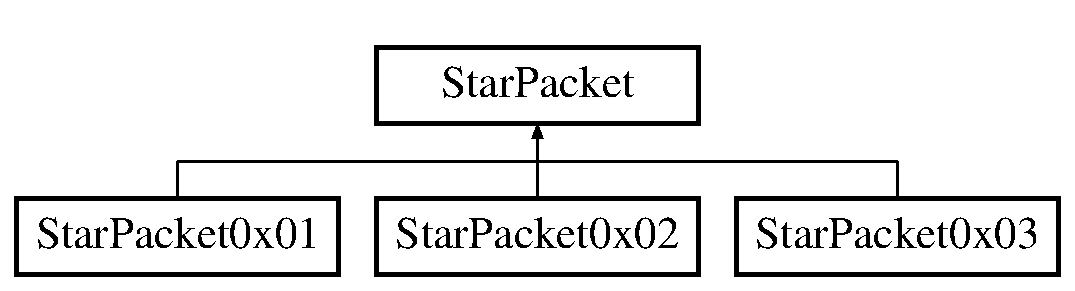
\includegraphics[height=2.000000cm]{classStarPacket}
\end{center}
\end{figure}
\subsection*{Public Member Functions}
\begin{DoxyCompactItemize}
\item 
\hyperlink{classStarPacket_a5d436c9e200c2c156da2dfeaac00898c}{Star\-Packet} ()
\item 
uint8\-\_\-t \hyperlink{classStarPacket_a61cf57919ceab8123336d74065f3aefe}{get\-Xid} ()
\end{DoxyCompactItemize}
\subsection*{Protected Attributes}
\begin{DoxyCompactItemize}
\item 
uint8\-\_\-t \hyperlink{classStarPacket_a3a2d6e31c97b1373736192282f8806f3}{xid}
\end{DoxyCompactItemize}


\subsection{Constructor \& Destructor Documentation}
\hypertarget{classStarPacket_a5d436c9e200c2c156da2dfeaac00898c}{\index{Star\-Packet@{Star\-Packet}!Star\-Packet@{Star\-Packet}}
\index{Star\-Packet@{Star\-Packet}!StarPacket@{Star\-Packet}}
\subsubsection[{Star\-Packet}]{\setlength{\rightskip}{0pt plus 5cm}Star\-Packet\-::\-Star\-Packet (
\begin{DoxyParamCaption}
{}
\end{DoxyParamCaption}
)\hspace{0.3cm}{\ttfamily [inline]}}}\label{classStarPacket_a5d436c9e200c2c156da2dfeaac00898c}


\subsection{Member Function Documentation}
\hypertarget{classStarPacket_a61cf57919ceab8123336d74065f3aefe}{\index{Star\-Packet@{Star\-Packet}!get\-Xid@{get\-Xid}}
\index{get\-Xid@{get\-Xid}!StarPacket@{Star\-Packet}}
\subsubsection[{get\-Xid}]{\setlength{\rightskip}{0pt plus 5cm}uint8\-\_\-t Star\-Packet\-::get\-Xid (
\begin{DoxyParamCaption}
{}
\end{DoxyParamCaption}
)\hspace{0.3cm}{\ttfamily [inline]}}}\label{classStarPacket_a61cf57919ceab8123336d74065f3aefe}


\subsection{Member Data Documentation}
\hypertarget{classStarPacket_a3a2d6e31c97b1373736192282f8806f3}{\index{Star\-Packet@{Star\-Packet}!xid@{xid}}
\index{xid@{xid}!StarPacket@{Star\-Packet}}
\subsubsection[{xid}]{\setlength{\rightskip}{0pt plus 5cm}uint8\-\_\-t Star\-Packet\-::xid\hspace{0.3cm}{\ttfamily [protected]}}}\label{classStarPacket_a3a2d6e31c97b1373736192282f8806f3}


The documentation for this class was generated from the following file\-:\begin{DoxyCompactItemize}
\item 
Resources/\-Star\-Packets/\hyperlink{StarPacket_8h}{Star\-Packet.\-h}\end{DoxyCompactItemize}

\hypertarget{classStarPacket0x01}{\section{Star\-Packet0x01 Class Reference}
\label{classStarPacket0x01}\index{Star\-Packet0x01@{Star\-Packet0x01}}
}


{\ttfamily \#include $<$Star\-Packet0x01.\-h$>$}

Inheritance diagram for Star\-Packet0x01\-:\begin{figure}[H]
\begin{center}
\leavevmode
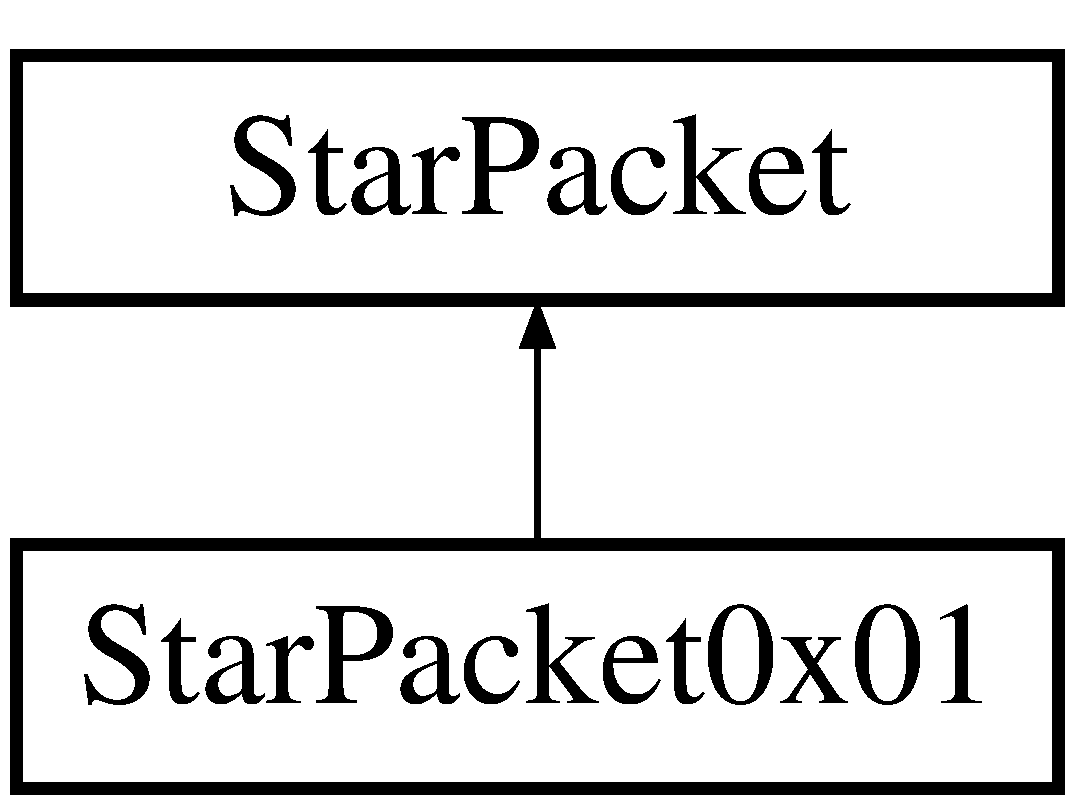
\includegraphics[height=2.000000cm]{classStarPacket0x01}
\end{center}
\end{figure}
\subsection*{Public Member Functions}
\begin{DoxyCompactItemize}
\item 
\hyperlink{classStarPacket0x01_a28be59db9b686a88a3cb7cdd5f42c78d}{Star\-Packet0x01} ()
\end{DoxyCompactItemize}
\subsection*{Additional Inherited Members}


\subsection{Constructor \& Destructor Documentation}
\hypertarget{classStarPacket0x01_a28be59db9b686a88a3cb7cdd5f42c78d}{\index{Star\-Packet0x01@{Star\-Packet0x01}!Star\-Packet0x01@{Star\-Packet0x01}}
\index{Star\-Packet0x01@{Star\-Packet0x01}!StarPacket0x01@{Star\-Packet0x01}}
\subsubsection[{Star\-Packet0x01}]{\setlength{\rightskip}{0pt plus 5cm}Star\-Packet0x01\-::\-Star\-Packet0x01 (
\begin{DoxyParamCaption}
{}
\end{DoxyParamCaption}
)}}\label{classStarPacket0x01_a28be59db9b686a88a3cb7cdd5f42c78d}


The documentation for this class was generated from the following file\-:\begin{DoxyCompactItemize}
\item 
Resources/\-Star\-Packets/\hyperlink{StarPacket0x01_8h}{Star\-Packet0x01.\-h}\end{DoxyCompactItemize}

\hypertarget{classStarPacket0x02}{\section{Star\-Packet0x02 Class Reference}
\label{classStarPacket0x02}\index{Star\-Packet0x02@{Star\-Packet0x02}}
}


{\ttfamily \#include $<$Star\-Packet0x02.\-h$>$}

Inheritance diagram for Star\-Packet0x02\-:\begin{figure}[H]
\begin{center}
\leavevmode
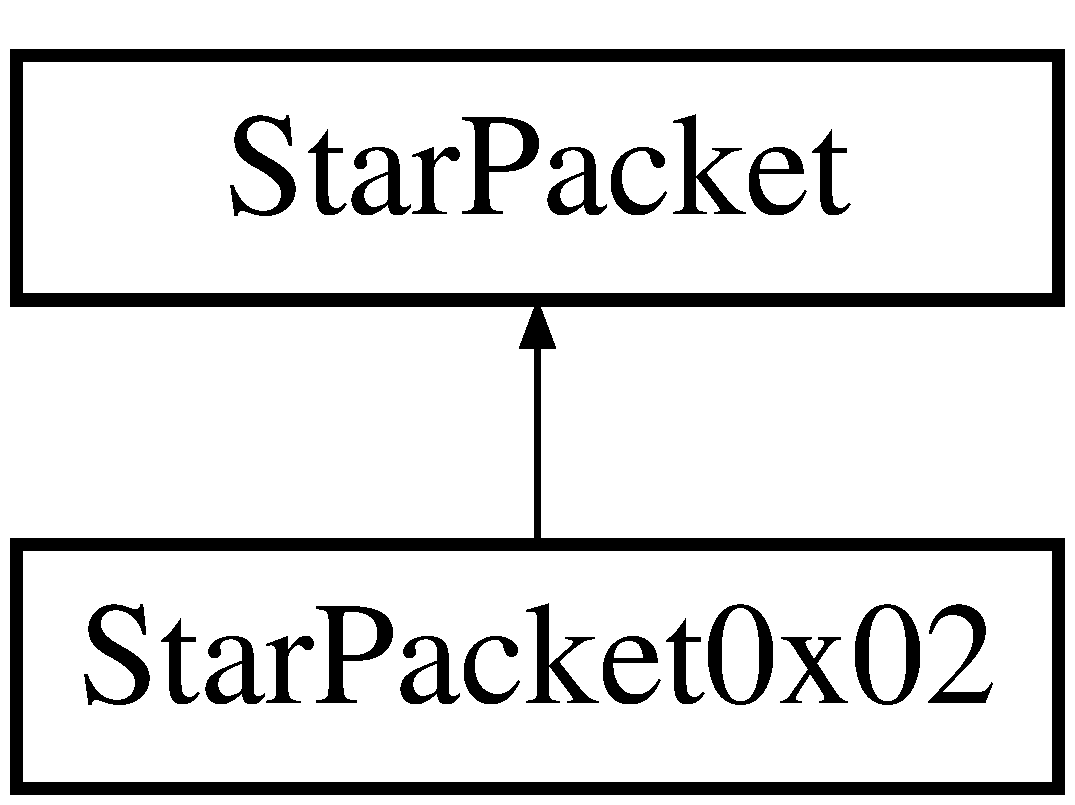
\includegraphics[height=2.000000cm]{classStarPacket0x02}
\end{center}
\end{figure}
\subsection*{Public Member Functions}
\begin{DoxyCompactItemize}
\item 
\hyperlink{classStarPacket0x02_a5b8f954734a2c921fbe1c89f50b57edd}{Star\-Packet0x02} ()
\end{DoxyCompactItemize}
\subsection*{Additional Inherited Members}


\subsection{Constructor \& Destructor Documentation}
\hypertarget{classStarPacket0x02_a5b8f954734a2c921fbe1c89f50b57edd}{\index{Star\-Packet0x02@{Star\-Packet0x02}!Star\-Packet0x02@{Star\-Packet0x02}}
\index{Star\-Packet0x02@{Star\-Packet0x02}!StarPacket0x02@{Star\-Packet0x02}}
\subsubsection[{Star\-Packet0x02}]{\setlength{\rightskip}{0pt plus 5cm}Star\-Packet0x02\-::\-Star\-Packet0x02 (
\begin{DoxyParamCaption}
{}
\end{DoxyParamCaption}
)}}\label{classStarPacket0x02_a5b8f954734a2c921fbe1c89f50b57edd}


The documentation for this class was generated from the following file\-:\begin{DoxyCompactItemize}
\item 
Resources/\-Star\-Packets/\hyperlink{StarPacket0x02_8h}{Star\-Packet0x02.\-h}\end{DoxyCompactItemize}

\hypertarget{classStarPacket0x03}{\section{Star\-Packet0x03 Class Reference}
\label{classStarPacket0x03}\index{Star\-Packet0x03@{Star\-Packet0x03}}
}


{\ttfamily \#include $<$Star\-Packet0x03.\-h$>$}

Inheritance diagram for Star\-Packet0x03\-:\begin{figure}[H]
\begin{center}
\leavevmode
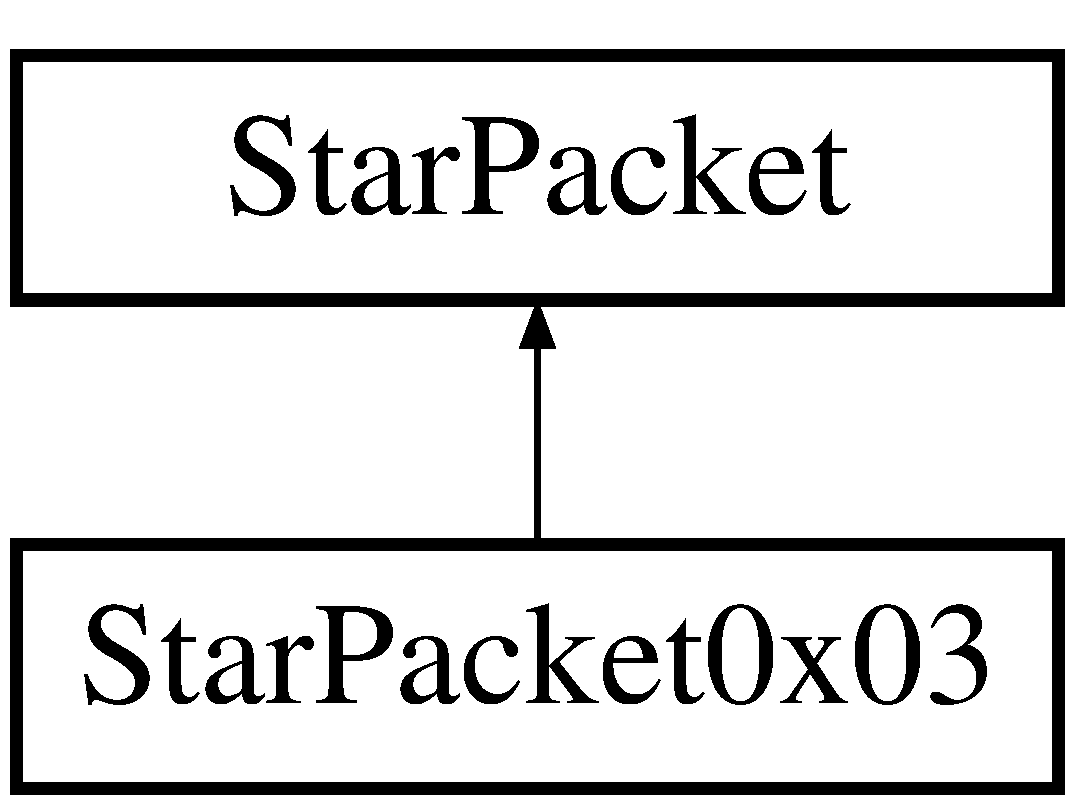
\includegraphics[height=2.000000cm]{classStarPacket0x03}
\end{center}
\end{figure}
\subsection*{Public Member Functions}
\begin{DoxyCompactItemize}
\item 
\hyperlink{classStarPacket0x03_aed9dca6ba0839be5cf7e8631dae40aa9}{Star\-Packet0x03} ()
\end{DoxyCompactItemize}
\subsection*{Additional Inherited Members}


\subsection{Constructor \& Destructor Documentation}
\hypertarget{classStarPacket0x03_aed9dca6ba0839be5cf7e8631dae40aa9}{\index{Star\-Packet0x03@{Star\-Packet0x03}!Star\-Packet0x03@{Star\-Packet0x03}}
\index{Star\-Packet0x03@{Star\-Packet0x03}!StarPacket0x03@{Star\-Packet0x03}}
\subsubsection[{Star\-Packet0x03}]{\setlength{\rightskip}{0pt plus 5cm}Star\-Packet0x03\-::\-Star\-Packet0x03 (
\begin{DoxyParamCaption}
{}
\end{DoxyParamCaption}
)}}\label{classStarPacket0x03_aed9dca6ba0839be5cf7e8631dae40aa9}


The documentation for this class was generated from the following file\-:\begin{DoxyCompactItemize}
\item 
Resources/\-Star\-Packets/\hyperlink{StarPacket0x03_8h}{Star\-Packet0x03.\-h}\end{DoxyCompactItemize}

\hypertarget{structSVMTrainParamsExt}{\section{S\-V\-M\-Train\-Params\-Ext Struct Reference}
\label{structSVMTrainParamsExt}\index{S\-V\-M\-Train\-Params\-Ext@{S\-V\-M\-Train\-Params\-Ext}}
}
\subsection*{Public Member Functions}
\begin{DoxyCompactItemize}
\item 
\hyperlink{structSVMTrainParamsExt_a0177ab89865d078f0fedb56752fc3233}{S\-V\-M\-Train\-Params\-Ext} ()
\item 
\hyperlink{structSVMTrainParamsExt_a3a15fad8802f7e367aeeea1eb92fcc0a}{S\-V\-M\-Train\-Params\-Ext} (float \-\_\-desc\-Percent, float \-\_\-target\-Ratio, bool \-\_\-balance\-Classes)
\item 
void \hyperlink{structSVMTrainParamsExt_a56e04fde17aa019cf1b64dc8631d412f}{read} (const File\-Node \&fn)
\item 
void \hyperlink{structSVMTrainParamsExt_a012f4fbdc13bb763f39e7d48c8f6f0eb}{write} (File\-Storage \&fs) const 
\item 
void \hyperlink{structSVMTrainParamsExt_a9413eed2aa93c88898e18d7c64037db9}{print} () const 
\end{DoxyCompactItemize}
\subsection*{Public Attributes}
\begin{DoxyCompactItemize}
\item 
float \hyperlink{structSVMTrainParamsExt_ad1203861c6c4a5a10403d3a2308d6d30}{desc\-Percent}
\item 
float \hyperlink{structSVMTrainParamsExt_a1e8099e1ff299cad8fe5c7fcf4e5fd07}{target\-Ratio}
\item 
bool \hyperlink{structSVMTrainParamsExt_a13677c5f8d3e2871193d01808ebf9726}{balance\-Classes}
\end{DoxyCompactItemize}


\subsection{Constructor \& Destructor Documentation}
\hypertarget{structSVMTrainParamsExt_a0177ab89865d078f0fedb56752fc3233}{\index{S\-V\-M\-Train\-Params\-Ext@{S\-V\-M\-Train\-Params\-Ext}!S\-V\-M\-Train\-Params\-Ext@{S\-V\-M\-Train\-Params\-Ext}}
\index{S\-V\-M\-Train\-Params\-Ext@{S\-V\-M\-Train\-Params\-Ext}!SVMTrainParamsExt@{S\-V\-M\-Train\-Params\-Ext}}
\subsubsection[{S\-V\-M\-Train\-Params\-Ext}]{\setlength{\rightskip}{0pt plus 5cm}S\-V\-M\-Train\-Params\-Ext\-::\-S\-V\-M\-Train\-Params\-Ext (
\begin{DoxyParamCaption}
{}
\end{DoxyParamCaption}
)\hspace{0.3cm}{\ttfamily [inline]}}}\label{structSVMTrainParamsExt_a0177ab89865d078f0fedb56752fc3233}
\hypertarget{structSVMTrainParamsExt_a3a15fad8802f7e367aeeea1eb92fcc0a}{\index{S\-V\-M\-Train\-Params\-Ext@{S\-V\-M\-Train\-Params\-Ext}!S\-V\-M\-Train\-Params\-Ext@{S\-V\-M\-Train\-Params\-Ext}}
\index{S\-V\-M\-Train\-Params\-Ext@{S\-V\-M\-Train\-Params\-Ext}!SVMTrainParamsExt@{S\-V\-M\-Train\-Params\-Ext}}
\subsubsection[{S\-V\-M\-Train\-Params\-Ext}]{\setlength{\rightskip}{0pt plus 5cm}S\-V\-M\-Train\-Params\-Ext\-::\-S\-V\-M\-Train\-Params\-Ext (
\begin{DoxyParamCaption}
\item[{float}]{\-\_\-desc\-Percent, }
\item[{float}]{\-\_\-target\-Ratio, }
\item[{bool}]{\-\_\-balance\-Classes}
\end{DoxyParamCaption}
)\hspace{0.3cm}{\ttfamily [inline]}}}\label{structSVMTrainParamsExt_a3a15fad8802f7e367aeeea1eb92fcc0a}


\subsection{Member Function Documentation}
\hypertarget{structSVMTrainParamsExt_a9413eed2aa93c88898e18d7c64037db9}{\index{S\-V\-M\-Train\-Params\-Ext@{S\-V\-M\-Train\-Params\-Ext}!print@{print}}
\index{print@{print}!SVMTrainParamsExt@{S\-V\-M\-Train\-Params\-Ext}}
\subsubsection[{print}]{\setlength{\rightskip}{0pt plus 5cm}void S\-V\-M\-Train\-Params\-Ext\-::print (
\begin{DoxyParamCaption}
{}
\end{DoxyParamCaption}
) const\hspace{0.3cm}{\ttfamily [inline]}}}\label{structSVMTrainParamsExt_a9413eed2aa93c88898e18d7c64037db9}
\hypertarget{structSVMTrainParamsExt_a56e04fde17aa019cf1b64dc8631d412f}{\index{S\-V\-M\-Train\-Params\-Ext@{S\-V\-M\-Train\-Params\-Ext}!read@{read}}
\index{read@{read}!SVMTrainParamsExt@{S\-V\-M\-Train\-Params\-Ext}}
\subsubsection[{read}]{\setlength{\rightskip}{0pt plus 5cm}void S\-V\-M\-Train\-Params\-Ext\-::read (
\begin{DoxyParamCaption}
\item[{const File\-Node \&}]{fn}
\end{DoxyParamCaption}
)\hspace{0.3cm}{\ttfamily [inline]}}}\label{structSVMTrainParamsExt_a56e04fde17aa019cf1b64dc8631d412f}
\hypertarget{structSVMTrainParamsExt_a012f4fbdc13bb763f39e7d48c8f6f0eb}{\index{S\-V\-M\-Train\-Params\-Ext@{S\-V\-M\-Train\-Params\-Ext}!write@{write}}
\index{write@{write}!SVMTrainParamsExt@{S\-V\-M\-Train\-Params\-Ext}}
\subsubsection[{write}]{\setlength{\rightskip}{0pt plus 5cm}void S\-V\-M\-Train\-Params\-Ext\-::write (
\begin{DoxyParamCaption}
\item[{File\-Storage \&}]{fs}
\end{DoxyParamCaption}
) const\hspace{0.3cm}{\ttfamily [inline]}}}\label{structSVMTrainParamsExt_a012f4fbdc13bb763f39e7d48c8f6f0eb}


\subsection{Member Data Documentation}
\hypertarget{structSVMTrainParamsExt_a13677c5f8d3e2871193d01808ebf9726}{\index{S\-V\-M\-Train\-Params\-Ext@{S\-V\-M\-Train\-Params\-Ext}!balance\-Classes@{balance\-Classes}}
\index{balance\-Classes@{balance\-Classes}!SVMTrainParamsExt@{S\-V\-M\-Train\-Params\-Ext}}
\subsubsection[{balance\-Classes}]{\setlength{\rightskip}{0pt plus 5cm}bool S\-V\-M\-Train\-Params\-Ext\-::balance\-Classes}}\label{structSVMTrainParamsExt_a13677c5f8d3e2871193d01808ebf9726}
\hypertarget{structSVMTrainParamsExt_ad1203861c6c4a5a10403d3a2308d6d30}{\index{S\-V\-M\-Train\-Params\-Ext@{S\-V\-M\-Train\-Params\-Ext}!desc\-Percent@{desc\-Percent}}
\index{desc\-Percent@{desc\-Percent}!SVMTrainParamsExt@{S\-V\-M\-Train\-Params\-Ext}}
\subsubsection[{desc\-Percent}]{\setlength{\rightskip}{0pt plus 5cm}float S\-V\-M\-Train\-Params\-Ext\-::desc\-Percent}}\label{structSVMTrainParamsExt_ad1203861c6c4a5a10403d3a2308d6d30}
\hypertarget{structSVMTrainParamsExt_a1e8099e1ff299cad8fe5c7fcf4e5fd07}{\index{S\-V\-M\-Train\-Params\-Ext@{S\-V\-M\-Train\-Params\-Ext}!target\-Ratio@{target\-Ratio}}
\index{target\-Ratio@{target\-Ratio}!SVMTrainParamsExt@{S\-V\-M\-Train\-Params\-Ext}}
\subsubsection[{target\-Ratio}]{\setlength{\rightskip}{0pt plus 5cm}float S\-V\-M\-Train\-Params\-Ext\-::target\-Ratio}}\label{structSVMTrainParamsExt_a1e8099e1ff299cad8fe5c7fcf4e5fd07}


The documentation for this struct was generated from the following file\-:\begin{DoxyCompactItemize}
\item 
Payload/\-A\-D\-L\-C/\-Shape\-Characterization/\-Open\-C\-V\-Example/\hyperlink{bagofwords__classification_8cpp}{bagofwords\-\_\-classification.\-cpp}\end{DoxyCompactItemize}

\hypertarget{structTarget}{\section{Target Struct Reference}
\label{structTarget}\index{Target@{Target}}
}


{\ttfamily \#include $<$Dimage.\-h$>$}

\subsection*{Public Attributes}
\begin{DoxyCompactItemize}
\item 
Mat \hyperlink{structTarget_ae37fee2ea260011ecacbfb0f23b3f9ab}{cropped\-Img}
\item 
Rect \hyperlink{structTarget_a7aeb05fae417de29ec649370007eba21}{coords}
\item 
char \hyperlink{structTarget_a489063b23f51649a9d16f988106021e3}{letter}
\item 
string \hyperlink{structTarget_adc3bbb55cca6bd906f5e8615a16d341e}{shape}
\item 
string \hyperlink{structTarget_a96b4e515aa265beb1996e430a4c5de07}{shape\-Color}
\item 
string \hyperlink{structTarget_acd28a79f6727170208e1a642e7471bc3}{letter\-Color}
\end{DoxyCompactItemize}


\subsection{Member Data Documentation}
\hypertarget{structTarget_a7aeb05fae417de29ec649370007eba21}{\index{Target@{Target}!coords@{coords}}
\index{coords@{coords}!Target@{Target}}
\subsubsection[{coords}]{\setlength{\rightskip}{0pt plus 5cm}Rect Target\-::coords}}\label{structTarget_a7aeb05fae417de29ec649370007eba21}
\hypertarget{structTarget_ae37fee2ea260011ecacbfb0f23b3f9ab}{\index{Target@{Target}!cropped\-Img@{cropped\-Img}}
\index{cropped\-Img@{cropped\-Img}!Target@{Target}}
\subsubsection[{cropped\-Img}]{\setlength{\rightskip}{0pt plus 5cm}Mat Target\-::cropped\-Img}}\label{structTarget_ae37fee2ea260011ecacbfb0f23b3f9ab}
\hypertarget{structTarget_a489063b23f51649a9d16f988106021e3}{\index{Target@{Target}!letter@{letter}}
\index{letter@{letter}!Target@{Target}}
\subsubsection[{letter}]{\setlength{\rightskip}{0pt plus 5cm}char Target\-::letter}}\label{structTarget_a489063b23f51649a9d16f988106021e3}
\hypertarget{structTarget_acd28a79f6727170208e1a642e7471bc3}{\index{Target@{Target}!letter\-Color@{letter\-Color}}
\index{letter\-Color@{letter\-Color}!Target@{Target}}
\subsubsection[{letter\-Color}]{\setlength{\rightskip}{0pt plus 5cm}string Target\-::letter\-Color}}\label{structTarget_acd28a79f6727170208e1a642e7471bc3}
\hypertarget{structTarget_adc3bbb55cca6bd906f5e8615a16d341e}{\index{Target@{Target}!shape@{shape}}
\index{shape@{shape}!Target@{Target}}
\subsubsection[{shape}]{\setlength{\rightskip}{0pt plus 5cm}string Target\-::shape}}\label{structTarget_adc3bbb55cca6bd906f5e8615a16d341e}
\hypertarget{structTarget_a96b4e515aa265beb1996e430a4c5de07}{\index{Target@{Target}!shape\-Color@{shape\-Color}}
\index{shape\-Color@{shape\-Color}!Target@{Target}}
\subsubsection[{shape\-Color}]{\setlength{\rightskip}{0pt plus 5cm}string Target\-::shape\-Color}}\label{structTarget_a96b4e515aa265beb1996e430a4c5de07}


The documentation for this struct was generated from the following file\-:\begin{DoxyCompactItemize}
\item 
Base\-Station/\-A\-D\-L\-C/inc/\hyperlink{BaseStation_2ADLC_2inc_2Dimage_8h}{Dimage.\-h}\end{DoxyCompactItemize}

\hypertarget{structVocabTrainParams}{\section{Vocab\-Train\-Params Struct Reference}
\label{structVocabTrainParams}\index{Vocab\-Train\-Params@{Vocab\-Train\-Params}}
}
\subsection*{Public Member Functions}
\begin{DoxyCompactItemize}
\item 
\hyperlink{structVocabTrainParams_a9d482783255ca8ae138f1eb22d0fc5fa}{Vocab\-Train\-Params} ()
\item 
\hyperlink{structVocabTrainParams_adbc39fcef1545755b8a32cd532546c02}{Vocab\-Train\-Params} (const string \-\_\-train\-Obj\-Class, size\-\_\-t \-\_\-vocab\-Size, size\-\_\-t \-\_\-memory\-Use, float \-\_\-desc\-Proportion)
\item 
void \hyperlink{structVocabTrainParams_aa4fb87c424b7644299f6967648181357}{read} (const File\-Node \&fn)
\item 
void \hyperlink{structVocabTrainParams_ac10429fab83898d30bc380257f5ac79c}{write} (File\-Storage \&fs) const 
\item 
void \hyperlink{structVocabTrainParams_a70613056f11a4b1ebea8542cb390f768}{print} () const 
\end{DoxyCompactItemize}
\subsection*{Public Attributes}
\begin{DoxyCompactItemize}
\item 
string \hyperlink{structVocabTrainParams_a091823486f23d578abfbc45c16ee01db}{train\-Obj\-Class}
\item 
int \hyperlink{structVocabTrainParams_af674926f696f54c5016aaca00c5df491}{vocab\-Size}
\item 
int \hyperlink{structVocabTrainParams_a496bcb5542cfbea6363fc058de4e200e}{memory\-Use}
\item 
float \hyperlink{structVocabTrainParams_a826922a4a2c21733527b3dc09d06d6d0}{desc\-Proportion}
\end{DoxyCompactItemize}


\subsection{Constructor \& Destructor Documentation}
\hypertarget{structVocabTrainParams_a9d482783255ca8ae138f1eb22d0fc5fa}{\index{Vocab\-Train\-Params@{Vocab\-Train\-Params}!Vocab\-Train\-Params@{Vocab\-Train\-Params}}
\index{Vocab\-Train\-Params@{Vocab\-Train\-Params}!VocabTrainParams@{Vocab\-Train\-Params}}
\subsubsection[{Vocab\-Train\-Params}]{\setlength{\rightskip}{0pt plus 5cm}Vocab\-Train\-Params\-::\-Vocab\-Train\-Params (
\begin{DoxyParamCaption}
{}
\end{DoxyParamCaption}
)\hspace{0.3cm}{\ttfamily [inline]}}}\label{structVocabTrainParams_a9d482783255ca8ae138f1eb22d0fc5fa}
\hypertarget{structVocabTrainParams_adbc39fcef1545755b8a32cd532546c02}{\index{Vocab\-Train\-Params@{Vocab\-Train\-Params}!Vocab\-Train\-Params@{Vocab\-Train\-Params}}
\index{Vocab\-Train\-Params@{Vocab\-Train\-Params}!VocabTrainParams@{Vocab\-Train\-Params}}
\subsubsection[{Vocab\-Train\-Params}]{\setlength{\rightskip}{0pt plus 5cm}Vocab\-Train\-Params\-::\-Vocab\-Train\-Params (
\begin{DoxyParamCaption}
\item[{const string}]{\-\_\-train\-Obj\-Class, }
\item[{size\-\_\-t}]{\-\_\-vocab\-Size, }
\item[{size\-\_\-t}]{\-\_\-memory\-Use, }
\item[{float}]{\-\_\-desc\-Proportion}
\end{DoxyParamCaption}
)\hspace{0.3cm}{\ttfamily [inline]}}}\label{structVocabTrainParams_adbc39fcef1545755b8a32cd532546c02}


\subsection{Member Function Documentation}
\hypertarget{structVocabTrainParams_a70613056f11a4b1ebea8542cb390f768}{\index{Vocab\-Train\-Params@{Vocab\-Train\-Params}!print@{print}}
\index{print@{print}!VocabTrainParams@{Vocab\-Train\-Params}}
\subsubsection[{print}]{\setlength{\rightskip}{0pt plus 5cm}void Vocab\-Train\-Params\-::print (
\begin{DoxyParamCaption}
{}
\end{DoxyParamCaption}
) const\hspace{0.3cm}{\ttfamily [inline]}}}\label{structVocabTrainParams_a70613056f11a4b1ebea8542cb390f768}
\hypertarget{structVocabTrainParams_aa4fb87c424b7644299f6967648181357}{\index{Vocab\-Train\-Params@{Vocab\-Train\-Params}!read@{read}}
\index{read@{read}!VocabTrainParams@{Vocab\-Train\-Params}}
\subsubsection[{read}]{\setlength{\rightskip}{0pt plus 5cm}void Vocab\-Train\-Params\-::read (
\begin{DoxyParamCaption}
\item[{const File\-Node \&}]{fn}
\end{DoxyParamCaption}
)\hspace{0.3cm}{\ttfamily [inline]}}}\label{structVocabTrainParams_aa4fb87c424b7644299f6967648181357}
\hypertarget{structVocabTrainParams_ac10429fab83898d30bc380257f5ac79c}{\index{Vocab\-Train\-Params@{Vocab\-Train\-Params}!write@{write}}
\index{write@{write}!VocabTrainParams@{Vocab\-Train\-Params}}
\subsubsection[{write}]{\setlength{\rightskip}{0pt plus 5cm}void Vocab\-Train\-Params\-::write (
\begin{DoxyParamCaption}
\item[{File\-Storage \&}]{fs}
\end{DoxyParamCaption}
) const\hspace{0.3cm}{\ttfamily [inline]}}}\label{structVocabTrainParams_ac10429fab83898d30bc380257f5ac79c}


\subsection{Member Data Documentation}
\hypertarget{structVocabTrainParams_a826922a4a2c21733527b3dc09d06d6d0}{\index{Vocab\-Train\-Params@{Vocab\-Train\-Params}!desc\-Proportion@{desc\-Proportion}}
\index{desc\-Proportion@{desc\-Proportion}!VocabTrainParams@{Vocab\-Train\-Params}}
\subsubsection[{desc\-Proportion}]{\setlength{\rightskip}{0pt plus 5cm}float Vocab\-Train\-Params\-::desc\-Proportion}}\label{structVocabTrainParams_a826922a4a2c21733527b3dc09d06d6d0}
\hypertarget{structVocabTrainParams_a496bcb5542cfbea6363fc058de4e200e}{\index{Vocab\-Train\-Params@{Vocab\-Train\-Params}!memory\-Use@{memory\-Use}}
\index{memory\-Use@{memory\-Use}!VocabTrainParams@{Vocab\-Train\-Params}}
\subsubsection[{memory\-Use}]{\setlength{\rightskip}{0pt plus 5cm}int Vocab\-Train\-Params\-::memory\-Use}}\label{structVocabTrainParams_a496bcb5542cfbea6363fc058de4e200e}
\hypertarget{structVocabTrainParams_a091823486f23d578abfbc45c16ee01db}{\index{Vocab\-Train\-Params@{Vocab\-Train\-Params}!train\-Obj\-Class@{train\-Obj\-Class}}
\index{train\-Obj\-Class@{train\-Obj\-Class}!VocabTrainParams@{Vocab\-Train\-Params}}
\subsubsection[{train\-Obj\-Class}]{\setlength{\rightskip}{0pt plus 5cm}string Vocab\-Train\-Params\-::train\-Obj\-Class}}\label{structVocabTrainParams_a091823486f23d578abfbc45c16ee01db}
\hypertarget{structVocabTrainParams_af674926f696f54c5016aaca00c5df491}{\index{Vocab\-Train\-Params@{Vocab\-Train\-Params}!vocab\-Size@{vocab\-Size}}
\index{vocab\-Size@{vocab\-Size}!VocabTrainParams@{Vocab\-Train\-Params}}
\subsubsection[{vocab\-Size}]{\setlength{\rightskip}{0pt plus 5cm}int Vocab\-Train\-Params\-::vocab\-Size}}\label{structVocabTrainParams_af674926f696f54c5016aaca00c5df491}


The documentation for this struct was generated from the following file\-:\begin{DoxyCompactItemize}
\item 
Payload/\-A\-D\-L\-C/\-Shape\-Characterization/\-Open\-C\-V\-Example/\hyperlink{bagofwords__classification_8cpp}{bagofwords\-\_\-classification.\-cpp}\end{DoxyCompactItemize}

\hypertarget{classVocData}{\section{Voc\-Data Class Reference}
\label{classVocData}\index{Voc\-Data@{Voc\-Data}}
}
\subsection*{Classes}
\begin{DoxyCompactItemize}
\item 
struct \hyperlink{structVocData_1_1orderingSorter}{ordering\-Sorter}
\end{DoxyCompactItemize}
\subsection*{Public Member Functions}
\begin{DoxyCompactItemize}
\item 
\hyperlink{classVocData_add6a2dc980a8e27ac39d6d03c08bc1cd}{Voc\-Data} (const string \&voc\-Path, bool use\-Test\-Dataset)
\item 
\hyperlink{classVocData_a575a2fec25b9ba78e6ff9bdc33336ad3}{$\sim$\-Voc\-Data} ()
\item 
void \hyperlink{classVocData_a92f58a9b3f73c2fbea3d80df27a5d1fc}{get\-Class\-Images} (const string \&obj\-\_\-class, const \hyperlink{bagofwords__classification_8cpp_a769a10790da271430ddd42e42073a0ea}{Obd\-Dataset\-Type} dataset, vector$<$ \hyperlink{classObdImage}{Obd\-Image} $>$ \&images, vector$<$ char $>$ \&object\-\_\-present)
\item 
void \hyperlink{classVocData_aee09184f35d00681609ff4605021a083}{get\-Class\-Objects} (const string \&obj\-\_\-class, const \hyperlink{bagofwords__classification_8cpp_a769a10790da271430ddd42e42073a0ea}{Obd\-Dataset\-Type} dataset, vector$<$ \hyperlink{classObdImage}{Obd\-Image} $>$ \&images, vector$<$ vector$<$ \hyperlink{classObdObject}{Obd\-Object} $>$ $>$ \&objects)
\item 
void \hyperlink{classVocData_a8ceef9c32fa3cbc4094e924c46732e9f}{get\-Class\-Objects} (const string \&obj\-\_\-class, const \hyperlink{bagofwords__classification_8cpp_a769a10790da271430ddd42e42073a0ea}{Obd\-Dataset\-Type} dataset, vector$<$ \hyperlink{classObdImage}{Obd\-Image} $>$ \&images, vector$<$ vector$<$ \hyperlink{classObdObject}{Obd\-Object} $>$ $>$ \&objects, vector$<$ vector$<$ \hyperlink{classVocObjectData}{Voc\-Object\-Data} $>$ $>$ \&object\-\_\-data, vector$<$ \hyperlink{bagofwords__classification_8cpp_a79995288ef1b2b5890517068e9bdfed8}{Voc\-G\-T} $>$ \&ground\-\_\-truth)
\item 
\hyperlink{classObdImage}{Obd\-Image} \hyperlink{classVocData_a6e4ecde19100ecfeb8c1f9afc12fc977}{get\-Objects} (const string \&id, vector$<$ \hyperlink{classObdObject}{Obd\-Object} $>$ \&objects)
\item 
\hyperlink{classObdImage}{Obd\-Image} \hyperlink{classVocData_a70c269f14e0e71abdc207c9910a74aab}{get\-Objects} (const string \&id, vector$<$ \hyperlink{classObdObject}{Obd\-Object} $>$ \&objects, vector$<$ \hyperlink{classVocObjectData}{Voc\-Object\-Data} $>$ \&object\-\_\-data)
\item 
\hyperlink{classObdImage}{Obd\-Image} \hyperlink{classVocData_a427c35f84d11424b071d5bfc11ac8fda}{get\-Objects} (const string \&obj\-\_\-class, const string \&id, vector$<$ \hyperlink{classObdObject}{Obd\-Object} $>$ \&objects, vector$<$ \hyperlink{classVocObjectData}{Voc\-Object\-Data} $>$ \&object\-\_\-data, \hyperlink{bagofwords__classification_8cpp_a79995288ef1b2b5890517068e9bdfed8}{Voc\-G\-T} \&ground\-\_\-truth)
\item 
void \hyperlink{classVocData_ab9527dd6557bf03b8fd253ae0066fa37}{get\-Classifier\-Ground\-Truth} (const string \&obj\-\_\-class, const vector$<$ \hyperlink{classObdImage}{Obd\-Image} $>$ \&images, vector$<$ char $>$ \&ground\-\_\-truth)
\item 
void \hyperlink{classVocData_ab90b59b732020d531a83bdf5afde7459}{get\-Classifier\-Ground\-Truth} (const string \&obj\-\_\-class, const vector$<$ string $>$ \&images, vector$<$ char $>$ \&ground\-\_\-truth)
\item 
int \hyperlink{classVocData_a95d562193b551c733fba22d2ca9fab3e}{get\-Detector\-Ground\-Truth} (const string \&obj\-\_\-class, const \hyperlink{bagofwords__classification_8cpp_a769a10790da271430ddd42e42073a0ea}{Obd\-Dataset\-Type} dataset, const vector$<$ \hyperlink{classObdImage}{Obd\-Image} $>$ \&images, const vector$<$ vector$<$ Rect $>$ $>$ \&bounding\-\_\-boxes, const vector$<$ vector$<$ float $>$ $>$ \&scores, vector$<$ vector$<$ char $>$ $>$ \&ground\-\_\-truth, vector$<$ vector$<$ char $>$ $>$ \&detection\-\_\-difficult, bool ignore\-\_\-difficult=true)
\item 
void \hyperlink{classVocData_a440a1a9cfd6e9ca080ce338f5c8a047d}{write\-Classifier\-Results\-File} (const string \&out\-\_\-dir, const string \&obj\-\_\-class, const \hyperlink{bagofwords__classification_8cpp_a769a10790da271430ddd42e42073a0ea}{Obd\-Dataset\-Type} dataset, const vector$<$ \hyperlink{classObdImage}{Obd\-Image} $>$ \&images, const vector$<$ float $>$ \&scores, const int competition=1, const bool overwrite\-\_\-ifexists=false)
\item 
string \hyperlink{classVocData_a50835c8bd8628e0d1ca61e3b3e8bc189}{get\-Results\-Filename} (const string \&obj\-\_\-class, const \hyperlink{bagofwords__classification_8cpp_a8453e90c379aabdea39070a17a9f63e2}{Voc\-Task} task, const \hyperlink{bagofwords__classification_8cpp_a769a10790da271430ddd42e42073a0ea}{Obd\-Dataset\-Type} dataset, const int competition=-\/1, const int number=-\/1)
\item 
void \hyperlink{classVocData_ac6dc007f256c36d8fe6ef395ed39dd8a}{calc\-Classifier\-Prec\-Recall} (const string \&obj\-\_\-class, const vector$<$ \hyperlink{classObdImage}{Obd\-Image} $>$ \&images, const vector$<$ float $>$ \&scores, vector$<$ float $>$ \&precision, vector$<$ float $>$ \&recall, float \&ap, vector$<$ size\-\_\-t $>$ \&ranking)
\item 
void \hyperlink{classVocData_aa1a71e116eabd997fe6fd76d0abe70a8}{calc\-Classifier\-Prec\-Recall} (const string \&obj\-\_\-class, const vector$<$ \hyperlink{classObdImage}{Obd\-Image} $>$ \&images, const vector$<$ float $>$ \&scores, vector$<$ float $>$ \&precision, vector$<$ float $>$ \&recall, float \&ap)
\item 
void \hyperlink{classVocData_a9e92b6a7403e18cf25df6165fd56a0bd}{calc\-Classifier\-Prec\-Recall} (const string \&input\-\_\-file, vector$<$ float $>$ \&precision, vector$<$ float $>$ \&recall, float \&ap, bool output\-Ranking\-File=false)
\item 
void \hyperlink{classVocData_ae8de46ec58d21ee43a44e8a771cbfaab}{calc\-Classifier\-Conf\-Mat\-Row} (const string \&obj\-\_\-class, const vector$<$ \hyperlink{classObdImage}{Obd\-Image} $>$ \&images, const vector$<$ float $>$ \&scores, const \hyperlink{bagofwords__classification_8cpp_a86b3fb0f82f82bd78e829cbb81032301}{Voc\-Conf\-Cond} cond, const float threshold, vector$<$ string $>$ \&output\-\_\-headers, vector$<$ float $>$ \&output\-\_\-values)
\item 
void \hyperlink{classVocData_a7b90894f21fbadf8aaf2c3eefa73fb8c}{calc\-Detector\-Conf\-Mat\-Row} (const string \&obj\-\_\-class, const \hyperlink{bagofwords__classification_8cpp_a769a10790da271430ddd42e42073a0ea}{Obd\-Dataset\-Type} dataset, const vector$<$ \hyperlink{classObdImage}{Obd\-Image} $>$ \&images, const vector$<$ vector$<$ float $>$ $>$ \&scores, const vector$<$ vector$<$ Rect $>$ $>$ \&bounding\-\_\-boxes, const \hyperlink{bagofwords__classification_8cpp_a86b3fb0f82f82bd78e829cbb81032301}{Voc\-Conf\-Cond} cond, const float threshold, vector$<$ string $>$ \&output\-\_\-headers, vector$<$ float $>$ \&output\-\_\-values, bool ignore\-\_\-difficult=true)
\item 
void \hyperlink{classVocData_aa6ac26da0ba7878beec8fb3598eaba96}{save\-Prec\-Recall\-To\-Gnuplot} (const string \&output\-\_\-file, const vector$<$ float $>$ \&precision, const vector$<$ float $>$ \&recall, const float ap, const string title=string(), const \hyperlink{bagofwords__classification_8cpp_a9d6bcb462c68f9c035a89cc559acb63f}{Voc\-Plot\-Type} plot\-\_\-type=\hyperlink{bagofwords__classification_8cpp_a9d6bcb462c68f9c035a89cc559acb63fac23aa01b33a316698ea57d9d594bf851}{C\-V\-\_\-\-V\-O\-C\-\_\-\-P\-L\-O\-T\-\_\-\-S\-C\-R\-E\-E\-N})
\item 
void \hyperlink{classVocData_a9580d183da05a4abd31a84699ab23302}{read\-Classifier\-Ground\-Truth} (const string \&obj\-\_\-class, const \hyperlink{bagofwords__classification_8cpp_a769a10790da271430ddd42e42073a0ea}{Obd\-Dataset\-Type} dataset, vector$<$ \hyperlink{classObdImage}{Obd\-Image} $>$ \&images, vector$<$ char $>$ \&object\-\_\-present)
\item 
void \hyperlink{classVocData_ad947e69a36f9569a2f479ac51786a365}{read\-Classifier\-Results\-File} (const std\-::string \&input\-\_\-file, vector$<$ \hyperlink{classObdImage}{Obd\-Image} $>$ \&images, vector$<$ float $>$ \&scores)
\item 
void \hyperlink{classVocData_aa09be545cbd6f37a76ba5d9d664bf402}{read\-Detector\-Results\-File} (const string \&input\-\_\-file, vector$<$ \hyperlink{classObdImage}{Obd\-Image} $>$ \&images, vector$<$ vector$<$ float $>$ $>$ \&scores, vector$<$ vector$<$ Rect $>$ $>$ \&bounding\-\_\-boxes)
\item 
const vector$<$ string $>$ \& \hyperlink{classVocData_a08fa5badaacbc8152ddb13bb3b27ea38}{get\-Object\-Classes} ()
\item 
string \hyperlink{classVocData_a87a3c312091a53dbd291f7b686d51d51}{get\-Results\-Directory} ()
\end{DoxyCompactItemize}
\subsection*{Protected Member Functions}
\begin{DoxyCompactItemize}
\item 
void \hyperlink{classVocData_ab71bb7378a0a0356d43492790f9ba187}{init\-Voc} (const string \&voc\-Path, const bool use\-Test\-Dataset)
\item 
void \hyperlink{classVocData_a26b0aee0bfa9621852db92d6fb5de147}{init\-Voc2007to2010} (const string \&voc\-Path, const bool use\-Test\-Dataset)
\item 
void \hyperlink{classVocData_a664471c4279bd2ac2e5bb6a0ef8de9c1}{read\-Classifier\-Ground\-Truth} (const string \&filename, vector$<$ string $>$ \&image\-\_\-codes, vector$<$ char $>$ \&object\-\_\-present)
\item 
void \hyperlink{classVocData_aac2d3f030a95224c8dafde8e2e4b3d06}{read\-Classifier\-Results\-File} (const string \&input\-\_\-file, vector$<$ string $>$ \&image\-\_\-codes, vector$<$ float $>$ \&scores)
\item 
void \hyperlink{classVocData_a4c31fa584e7b47c578d44376e2ef8e86}{read\-Detector\-Results\-File} (const string \&input\-\_\-file, vector$<$ string $>$ \&image\-\_\-codes, vector$<$ vector$<$ float $>$ $>$ \&scores, vector$<$ vector$<$ Rect $>$ $>$ \&bounding\-\_\-boxes)
\item 
void \hyperlink{classVocData_a1a41aa13a88461655386bb1225853df7}{extract\-Voc\-Objects} (const string filename, vector$<$ \hyperlink{classObdObject}{Obd\-Object} $>$ \&objects, vector$<$ \hyperlink{classVocObjectData}{Voc\-Object\-Data} $>$ \&object\-\_\-data)
\item 
string \hyperlink{classVocData_a752e19ab7762411e1e8697cf708b1595}{get\-Image\-Path} (const string \&input\-\_\-str)
\item 
void \hyperlink{classVocData_ae153b6a3a13738cf35b1c264028de279}{get\-Class\-Images\-\_\-impl} (const string \&obj\-\_\-class, const string \&dataset\-\_\-str, vector$<$ \hyperlink{classObdImage}{Obd\-Image} $>$ \&images, vector$<$ char $>$ \&object\-\_\-present)
\item 
void \hyperlink{classVocData_af04f6b1b7d377efb8022416cb7c2452a}{calc\-Prec\-Recall\-\_\-impl} (const vector$<$ char $>$ \&ground\-\_\-truth, const vector$<$ float $>$ \&scores, vector$<$ float $>$ \&precision, vector$<$ float $>$ \&recall, float \&ap, vector$<$ size\-\_\-t $>$ \&ranking, int recall\-\_\-normalization=-\/1)
\item 
float \hyperlink{classVocData_a1cbbaf80dd0d3180a94868c1bdc5b3b5}{test\-Bounding\-Boxes\-For\-Overlap} (const Rect detection, const Rect ground\-\_\-truth)
\item 
void \hyperlink{classVocData_a12f52ec04b326eed957b02883f8da836}{extract\-Data\-From\-Results\-Filename} (const string \&input\-\_\-file, string \&class\-\_\-name, string \&dataset\-\_\-name)
\item 
bool \hyperlink{classVocData_a1d313e61c54cf27ec2500b38d9f16eda}{get\-Classifier\-Ground\-Truth\-Image} (const string \&obj\-\_\-class, const string \&id)
\item 
void \hyperlink{classVocData_aecc9f83f5e0ab63fc09e60679982342d}{get\-Sort\-Order} (const vector$<$ float $>$ \&values, vector$<$ size\-\_\-t $>$ \&order, bool descending=true)
\item 
int \hyperlink{classVocData_aecd0e31768fb9a202224d0dde4a05178}{string\-To\-Integer} (const string input\-\_\-str)
\item 
void \hyperlink{classVocData_aa556074b41f8f5a1ac611b6b4fa06c2d}{read\-File\-To\-String} (const string filename, string \&file\-\_\-contents)
\item 
string \hyperlink{classVocData_afcc3d337fc5c33e53cdaef5f8589ac1d}{integer\-To\-String} (const int input\-\_\-int)
\item 
string \hyperlink{classVocData_a33d4a839f14d65bc5f4bdb4e89d625d1}{check\-Filename\-Pathsep} (const string filename, bool add\-\_\-trailing\-\_\-slash=false)
\item 
void \hyperlink{classVocData_a9542ea7c7c7d2f500637b7e4dbee8de8}{convert\-Image\-Codes\-To\-Obd\-Images} (const vector$<$ string $>$ \&image\-\_\-codes, vector$<$ \hyperlink{classObdImage}{Obd\-Image} $>$ \&images)
\item 
int \hyperlink{classVocData_a9509a28cfed76d7f8a4c1768462a01a9}{extract\-X\-M\-L\-Block} (const string src, const string tag, const int searchpos, string \&tag\-\_\-contents)
\end{DoxyCompactItemize}
\subsection*{Protected Attributes}
\begin{DoxyCompactItemize}
\item 
string \hyperlink{classVocData_ab5991ec812cb9c53716188ea67f52e51}{m\-\_\-voc\-Path}
\item 
string \hyperlink{classVocData_a292154bce82b205ce3946d7c66be9dff}{m\-\_\-voc\-Name}
\item 
string \hyperlink{classVocData_a4cea52c78090ef0d0c7ac380221802ab}{m\-\_\-annotation\-\_\-path}
\item 
string \hyperlink{classVocData_abab33911d384984e37e91b8ae1217f05}{m\-\_\-image\-\_\-path}
\item 
string \hyperlink{classVocData_af2aae5c6b4b430d3bf098f9557daea6a}{m\-\_\-imageset\-\_\-path}
\item 
string \hyperlink{classVocData_a456472463a937a9da9fd723b5aae65b8}{m\-\_\-class\-\_\-imageset\-\_\-path}
\item 
vector$<$ string $>$ \hyperlink{classVocData_aafde0db81fa35c5d46c4ce06b460b78e}{m\-\_\-classifier\-\_\-gt\-\_\-all\-\_\-ids}
\item 
vector$<$ char $>$ \hyperlink{classVocData_a02141120f0e5086a4f53113409b6d159}{m\-\_\-classifier\-\_\-gt\-\_\-all\-\_\-present}
\item 
string \hyperlink{classVocData_a35fe10bbcca7681acc0365cb18ca3920}{m\-\_\-classifier\-\_\-gt\-\_\-class}
\item 
string \hyperlink{classVocData_a6e63a9455ea3a21e08a493c5c2f26b5a}{m\-\_\-train\-\_\-set}
\item 
string \hyperlink{classVocData_ace1c925120f1b37c1fe536350aa42346}{m\-\_\-test\-\_\-set}
\item 
vector$<$ string $>$ \hyperlink{classVocData_a3b6160c9706be61b4abe53a2d672ca76}{m\-\_\-object\-\_\-classes}
\item 
float \hyperlink{classVocData_a8f6be5bd01a56f1fdf3ff6a1756e1ff6}{m\-\_\-min\-\_\-overlap}
\item 
bool \hyperlink{classVocData_a90dc858323c9074eef60dd14aebb611e}{m\-\_\-sampled\-\_\-ap}
\end{DoxyCompactItemize}


\subsection{Constructor \& Destructor Documentation}
\hypertarget{classVocData_add6a2dc980a8e27ac39d6d03c08bc1cd}{\index{Voc\-Data@{Voc\-Data}!Voc\-Data@{Voc\-Data}}
\index{Voc\-Data@{Voc\-Data}!VocData@{Voc\-Data}}
\subsubsection[{Voc\-Data}]{\setlength{\rightskip}{0pt plus 5cm}Voc\-Data\-::\-Voc\-Data (
\begin{DoxyParamCaption}
\item[{const string \&}]{voc\-Path, }
\item[{bool}]{use\-Test\-Dataset}
\end{DoxyParamCaption}
)\hspace{0.3cm}{\ttfamily [inline]}}}\label{classVocData_add6a2dc980a8e27ac39d6d03c08bc1cd}
\hypertarget{classVocData_a575a2fec25b9ba78e6ff9bdc33336ad3}{\index{Voc\-Data@{Voc\-Data}!$\sim$\-Voc\-Data@{$\sim$\-Voc\-Data}}
\index{$\sim$\-Voc\-Data@{$\sim$\-Voc\-Data}!VocData@{Voc\-Data}}
\subsubsection[{$\sim$\-Voc\-Data}]{\setlength{\rightskip}{0pt plus 5cm}Voc\-Data\-::$\sim$\-Voc\-Data (
\begin{DoxyParamCaption}
{}
\end{DoxyParamCaption}
)\hspace{0.3cm}{\ttfamily [inline]}}}\label{classVocData_a575a2fec25b9ba78e6ff9bdc33336ad3}


\subsection{Member Function Documentation}
\hypertarget{classVocData_ae8de46ec58d21ee43a44e8a771cbfaab}{\index{Voc\-Data@{Voc\-Data}!calc\-Classifier\-Conf\-Mat\-Row@{calc\-Classifier\-Conf\-Mat\-Row}}
\index{calc\-Classifier\-Conf\-Mat\-Row@{calc\-Classifier\-Conf\-Mat\-Row}!VocData@{Voc\-Data}}
\subsubsection[{calc\-Classifier\-Conf\-Mat\-Row}]{\setlength{\rightskip}{0pt plus 5cm}void Voc\-Data\-::calc\-Classifier\-Conf\-Mat\-Row (
\begin{DoxyParamCaption}
\item[{const string \&}]{obj\-\_\-class, }
\item[{const vector$<$ {\bf Obd\-Image} $>$ \&}]{images, }
\item[{const vector$<$ float $>$ \&}]{scores, }
\item[{const {\bf Voc\-Conf\-Cond}}]{cond, }
\item[{const float}]{threshold, }
\item[{vector$<$ string $>$ \&}]{output\-\_\-headers, }
\item[{vector$<$ float $>$ \&}]{output\-\_\-values}
\end{DoxyParamCaption}
)}}\label{classVocData_ae8de46ec58d21ee43a44e8a771cbfaab}
\hypertarget{classVocData_ac6dc007f256c36d8fe6ef395ed39dd8a}{\index{Voc\-Data@{Voc\-Data}!calc\-Classifier\-Prec\-Recall@{calc\-Classifier\-Prec\-Recall}}
\index{calc\-Classifier\-Prec\-Recall@{calc\-Classifier\-Prec\-Recall}!VocData@{Voc\-Data}}
\subsubsection[{calc\-Classifier\-Prec\-Recall}]{\setlength{\rightskip}{0pt plus 5cm}void Voc\-Data\-::calc\-Classifier\-Prec\-Recall (
\begin{DoxyParamCaption}
\item[{const string \&}]{obj\-\_\-class, }
\item[{const vector$<$ {\bf Obd\-Image} $>$ \&}]{images, }
\item[{const vector$<$ float $>$ \&}]{scores, }
\item[{vector$<$ float $>$ \&}]{precision, }
\item[{vector$<$ float $>$ \&}]{recall, }
\item[{float \&}]{ap, }
\item[{vector$<$ size\-\_\-t $>$ \&}]{ranking}
\end{DoxyParamCaption}
)}}\label{classVocData_ac6dc007f256c36d8fe6ef395ed39dd8a}
\hypertarget{classVocData_aa1a71e116eabd997fe6fd76d0abe70a8}{\index{Voc\-Data@{Voc\-Data}!calc\-Classifier\-Prec\-Recall@{calc\-Classifier\-Prec\-Recall}}
\index{calc\-Classifier\-Prec\-Recall@{calc\-Classifier\-Prec\-Recall}!VocData@{Voc\-Data}}
\subsubsection[{calc\-Classifier\-Prec\-Recall}]{\setlength{\rightskip}{0pt plus 5cm}void Voc\-Data\-::calc\-Classifier\-Prec\-Recall (
\begin{DoxyParamCaption}
\item[{const string \&}]{obj\-\_\-class, }
\item[{const vector$<$ {\bf Obd\-Image} $>$ \&}]{images, }
\item[{const vector$<$ float $>$ \&}]{scores, }
\item[{vector$<$ float $>$ \&}]{precision, }
\item[{vector$<$ float $>$ \&}]{recall, }
\item[{float \&}]{ap}
\end{DoxyParamCaption}
)}}\label{classVocData_aa1a71e116eabd997fe6fd76d0abe70a8}
\hypertarget{classVocData_a9e92b6a7403e18cf25df6165fd56a0bd}{\index{Voc\-Data@{Voc\-Data}!calc\-Classifier\-Prec\-Recall@{calc\-Classifier\-Prec\-Recall}}
\index{calc\-Classifier\-Prec\-Recall@{calc\-Classifier\-Prec\-Recall}!VocData@{Voc\-Data}}
\subsubsection[{calc\-Classifier\-Prec\-Recall}]{\setlength{\rightskip}{0pt plus 5cm}void Voc\-Data\-::calc\-Classifier\-Prec\-Recall (
\begin{DoxyParamCaption}
\item[{const string \&}]{input\-\_\-file, }
\item[{vector$<$ float $>$ \&}]{precision, }
\item[{vector$<$ float $>$ \&}]{recall, }
\item[{float \&}]{ap, }
\item[{bool}]{output\-Ranking\-File = {\ttfamily false}}
\end{DoxyParamCaption}
)}}\label{classVocData_a9e92b6a7403e18cf25df6165fd56a0bd}
\hypertarget{classVocData_a7b90894f21fbadf8aaf2c3eefa73fb8c}{\index{Voc\-Data@{Voc\-Data}!calc\-Detector\-Conf\-Mat\-Row@{calc\-Detector\-Conf\-Mat\-Row}}
\index{calc\-Detector\-Conf\-Mat\-Row@{calc\-Detector\-Conf\-Mat\-Row}!VocData@{Voc\-Data}}
\subsubsection[{calc\-Detector\-Conf\-Mat\-Row}]{\setlength{\rightskip}{0pt plus 5cm}void Voc\-Data\-::calc\-Detector\-Conf\-Mat\-Row (
\begin{DoxyParamCaption}
\item[{const string \&}]{obj\-\_\-class, }
\item[{const {\bf Obd\-Dataset\-Type}}]{dataset, }
\item[{const vector$<$ {\bf Obd\-Image} $>$ \&}]{images, }
\item[{const vector$<$ vector$<$ float $>$ $>$ \&}]{scores, }
\item[{const vector$<$ vector$<$ Rect $>$ $>$ \&}]{bounding\-\_\-boxes, }
\item[{const {\bf Voc\-Conf\-Cond}}]{cond, }
\item[{const float}]{threshold, }
\item[{vector$<$ string $>$ \&}]{output\-\_\-headers, }
\item[{vector$<$ float $>$ \&}]{output\-\_\-values, }
\item[{bool}]{ignore\-\_\-difficult = {\ttfamily true}}
\end{DoxyParamCaption}
)}}\label{classVocData_a7b90894f21fbadf8aaf2c3eefa73fb8c}
\hypertarget{classVocData_af04f6b1b7d377efb8022416cb7c2452a}{\index{Voc\-Data@{Voc\-Data}!calc\-Prec\-Recall\-\_\-impl@{calc\-Prec\-Recall\-\_\-impl}}
\index{calc\-Prec\-Recall\-\_\-impl@{calc\-Prec\-Recall\-\_\-impl}!VocData@{Voc\-Data}}
\subsubsection[{calc\-Prec\-Recall\-\_\-impl}]{\setlength{\rightskip}{0pt plus 5cm}void Voc\-Data\-::calc\-Prec\-Recall\-\_\-impl (
\begin{DoxyParamCaption}
\item[{const vector$<$ char $>$ \&}]{ground\-\_\-truth, }
\item[{const vector$<$ float $>$ \&}]{scores, }
\item[{vector$<$ float $>$ \&}]{precision, }
\item[{vector$<$ float $>$ \&}]{recall, }
\item[{float \&}]{ap, }
\item[{vector$<$ size\-\_\-t $>$ \&}]{ranking, }
\item[{int}]{recall\-\_\-normalization = {\ttfamily -\/1}}
\end{DoxyParamCaption}
)\hspace{0.3cm}{\ttfamily [protected]}}}\label{classVocData_af04f6b1b7d377efb8022416cb7c2452a}
\hypertarget{classVocData_a33d4a839f14d65bc5f4bdb4e89d625d1}{\index{Voc\-Data@{Voc\-Data}!check\-Filename\-Pathsep@{check\-Filename\-Pathsep}}
\index{check\-Filename\-Pathsep@{check\-Filename\-Pathsep}!VocData@{Voc\-Data}}
\subsubsection[{check\-Filename\-Pathsep}]{\setlength{\rightskip}{0pt plus 5cm}string Voc\-Data\-::check\-Filename\-Pathsep (
\begin{DoxyParamCaption}
\item[{const string}]{filename, }
\item[{bool}]{add\-\_\-trailing\-\_\-slash = {\ttfamily false}}
\end{DoxyParamCaption}
)\hspace{0.3cm}{\ttfamily [protected]}}}\label{classVocData_a33d4a839f14d65bc5f4bdb4e89d625d1}
\hypertarget{classVocData_a9542ea7c7c7d2f500637b7e4dbee8de8}{\index{Voc\-Data@{Voc\-Data}!convert\-Image\-Codes\-To\-Obd\-Images@{convert\-Image\-Codes\-To\-Obd\-Images}}
\index{convert\-Image\-Codes\-To\-Obd\-Images@{convert\-Image\-Codes\-To\-Obd\-Images}!VocData@{Voc\-Data}}
\subsubsection[{convert\-Image\-Codes\-To\-Obd\-Images}]{\setlength{\rightskip}{0pt plus 5cm}void Voc\-Data\-::convert\-Image\-Codes\-To\-Obd\-Images (
\begin{DoxyParamCaption}
\item[{const vector$<$ string $>$ \&}]{image\-\_\-codes, }
\item[{vector$<$ {\bf Obd\-Image} $>$ \&}]{images}
\end{DoxyParamCaption}
)\hspace{0.3cm}{\ttfamily [protected]}}}\label{classVocData_a9542ea7c7c7d2f500637b7e4dbee8de8}
\hypertarget{classVocData_a12f52ec04b326eed957b02883f8da836}{\index{Voc\-Data@{Voc\-Data}!extract\-Data\-From\-Results\-Filename@{extract\-Data\-From\-Results\-Filename}}
\index{extract\-Data\-From\-Results\-Filename@{extract\-Data\-From\-Results\-Filename}!VocData@{Voc\-Data}}
\subsubsection[{extract\-Data\-From\-Results\-Filename}]{\setlength{\rightskip}{0pt plus 5cm}void Voc\-Data\-::extract\-Data\-From\-Results\-Filename (
\begin{DoxyParamCaption}
\item[{const string \&}]{input\-\_\-file, }
\item[{string \&}]{class\-\_\-name, }
\item[{string \&}]{dataset\-\_\-name}
\end{DoxyParamCaption}
)\hspace{0.3cm}{\ttfamily [protected]}}}\label{classVocData_a12f52ec04b326eed957b02883f8da836}
\hypertarget{classVocData_a1a41aa13a88461655386bb1225853df7}{\index{Voc\-Data@{Voc\-Data}!extract\-Voc\-Objects@{extract\-Voc\-Objects}}
\index{extract\-Voc\-Objects@{extract\-Voc\-Objects}!VocData@{Voc\-Data}}
\subsubsection[{extract\-Voc\-Objects}]{\setlength{\rightskip}{0pt plus 5cm}void Voc\-Data\-::extract\-Voc\-Objects (
\begin{DoxyParamCaption}
\item[{const string}]{filename, }
\item[{vector$<$ {\bf Obd\-Object} $>$ \&}]{objects, }
\item[{vector$<$ {\bf Voc\-Object\-Data} $>$ \&}]{object\-\_\-data}
\end{DoxyParamCaption}
)\hspace{0.3cm}{\ttfamily [protected]}}}\label{classVocData_a1a41aa13a88461655386bb1225853df7}
\hypertarget{classVocData_a9509a28cfed76d7f8a4c1768462a01a9}{\index{Voc\-Data@{Voc\-Data}!extract\-X\-M\-L\-Block@{extract\-X\-M\-L\-Block}}
\index{extract\-X\-M\-L\-Block@{extract\-X\-M\-L\-Block}!VocData@{Voc\-Data}}
\subsubsection[{extract\-X\-M\-L\-Block}]{\setlength{\rightskip}{0pt plus 5cm}int Voc\-Data\-::extract\-X\-M\-L\-Block (
\begin{DoxyParamCaption}
\item[{const string}]{src, }
\item[{const string}]{tag, }
\item[{const int}]{searchpos, }
\item[{string \&}]{tag\-\_\-contents}
\end{DoxyParamCaption}
)\hspace{0.3cm}{\ttfamily [protected]}}}\label{classVocData_a9509a28cfed76d7f8a4c1768462a01a9}
\hypertarget{classVocData_ab9527dd6557bf03b8fd253ae0066fa37}{\index{Voc\-Data@{Voc\-Data}!get\-Classifier\-Ground\-Truth@{get\-Classifier\-Ground\-Truth}}
\index{get\-Classifier\-Ground\-Truth@{get\-Classifier\-Ground\-Truth}!VocData@{Voc\-Data}}
\subsubsection[{get\-Classifier\-Ground\-Truth}]{\setlength{\rightskip}{0pt plus 5cm}void Voc\-Data\-::get\-Classifier\-Ground\-Truth (
\begin{DoxyParamCaption}
\item[{const string \&}]{obj\-\_\-class, }
\item[{const vector$<$ {\bf Obd\-Image} $>$ \&}]{images, }
\item[{vector$<$ char $>$ \&}]{ground\-\_\-truth}
\end{DoxyParamCaption}
)}}\label{classVocData_ab9527dd6557bf03b8fd253ae0066fa37}
\hypertarget{classVocData_ab90b59b732020d531a83bdf5afde7459}{\index{Voc\-Data@{Voc\-Data}!get\-Classifier\-Ground\-Truth@{get\-Classifier\-Ground\-Truth}}
\index{get\-Classifier\-Ground\-Truth@{get\-Classifier\-Ground\-Truth}!VocData@{Voc\-Data}}
\subsubsection[{get\-Classifier\-Ground\-Truth}]{\setlength{\rightskip}{0pt plus 5cm}void Voc\-Data\-::get\-Classifier\-Ground\-Truth (
\begin{DoxyParamCaption}
\item[{const string \&}]{obj\-\_\-class, }
\item[{const vector$<$ string $>$ \&}]{images, }
\item[{vector$<$ char $>$ \&}]{ground\-\_\-truth}
\end{DoxyParamCaption}
)}}\label{classVocData_ab90b59b732020d531a83bdf5afde7459}
\hypertarget{classVocData_a1d313e61c54cf27ec2500b38d9f16eda}{\index{Voc\-Data@{Voc\-Data}!get\-Classifier\-Ground\-Truth\-Image@{get\-Classifier\-Ground\-Truth\-Image}}
\index{get\-Classifier\-Ground\-Truth\-Image@{get\-Classifier\-Ground\-Truth\-Image}!VocData@{Voc\-Data}}
\subsubsection[{get\-Classifier\-Ground\-Truth\-Image}]{\setlength{\rightskip}{0pt plus 5cm}bool Voc\-Data\-::get\-Classifier\-Ground\-Truth\-Image (
\begin{DoxyParamCaption}
\item[{const string \&}]{obj\-\_\-class, }
\item[{const string \&}]{id}
\end{DoxyParamCaption}
)\hspace{0.3cm}{\ttfamily [protected]}}}\label{classVocData_a1d313e61c54cf27ec2500b38d9f16eda}
\hypertarget{classVocData_a92f58a9b3f73c2fbea3d80df27a5d1fc}{\index{Voc\-Data@{Voc\-Data}!get\-Class\-Images@{get\-Class\-Images}}
\index{get\-Class\-Images@{get\-Class\-Images}!VocData@{Voc\-Data}}
\subsubsection[{get\-Class\-Images}]{\setlength{\rightskip}{0pt plus 5cm}void Voc\-Data\-::get\-Class\-Images (
\begin{DoxyParamCaption}
\item[{const string \&}]{obj\-\_\-class, }
\item[{const {\bf Obd\-Dataset\-Type}}]{dataset, }
\item[{vector$<$ {\bf Obd\-Image} $>$ \&}]{images, }
\item[{vector$<$ char $>$ \&}]{object\-\_\-present}
\end{DoxyParamCaption}
)}}\label{classVocData_a92f58a9b3f73c2fbea3d80df27a5d1fc}
\hypertarget{classVocData_ae153b6a3a13738cf35b1c264028de279}{\index{Voc\-Data@{Voc\-Data}!get\-Class\-Images\-\_\-impl@{get\-Class\-Images\-\_\-impl}}
\index{get\-Class\-Images\-\_\-impl@{get\-Class\-Images\-\_\-impl}!VocData@{Voc\-Data}}
\subsubsection[{get\-Class\-Images\-\_\-impl}]{\setlength{\rightskip}{0pt plus 5cm}void Voc\-Data\-::get\-Class\-Images\-\_\-impl (
\begin{DoxyParamCaption}
\item[{const string \&}]{obj\-\_\-class, }
\item[{const string \&}]{dataset\-\_\-str, }
\item[{vector$<$ {\bf Obd\-Image} $>$ \&}]{images, }
\item[{vector$<$ char $>$ \&}]{object\-\_\-present}
\end{DoxyParamCaption}
)\hspace{0.3cm}{\ttfamily [protected]}}}\label{classVocData_ae153b6a3a13738cf35b1c264028de279}
\hypertarget{classVocData_aee09184f35d00681609ff4605021a083}{\index{Voc\-Data@{Voc\-Data}!get\-Class\-Objects@{get\-Class\-Objects}}
\index{get\-Class\-Objects@{get\-Class\-Objects}!VocData@{Voc\-Data}}
\subsubsection[{get\-Class\-Objects}]{\setlength{\rightskip}{0pt plus 5cm}void Voc\-Data\-::get\-Class\-Objects (
\begin{DoxyParamCaption}
\item[{const string \&}]{obj\-\_\-class, }
\item[{const {\bf Obd\-Dataset\-Type}}]{dataset, }
\item[{vector$<$ {\bf Obd\-Image} $>$ \&}]{images, }
\item[{vector$<$ vector$<$ {\bf Obd\-Object} $>$ $>$ \&}]{objects}
\end{DoxyParamCaption}
)}}\label{classVocData_aee09184f35d00681609ff4605021a083}
\hypertarget{classVocData_a8ceef9c32fa3cbc4094e924c46732e9f}{\index{Voc\-Data@{Voc\-Data}!get\-Class\-Objects@{get\-Class\-Objects}}
\index{get\-Class\-Objects@{get\-Class\-Objects}!VocData@{Voc\-Data}}
\subsubsection[{get\-Class\-Objects}]{\setlength{\rightskip}{0pt plus 5cm}void Voc\-Data\-::get\-Class\-Objects (
\begin{DoxyParamCaption}
\item[{const string \&}]{obj\-\_\-class, }
\item[{const {\bf Obd\-Dataset\-Type}}]{dataset, }
\item[{vector$<$ {\bf Obd\-Image} $>$ \&}]{images, }
\item[{vector$<$ vector$<$ {\bf Obd\-Object} $>$ $>$ \&}]{objects, }
\item[{vector$<$ vector$<$ {\bf Voc\-Object\-Data} $>$ $>$ \&}]{object\-\_\-data, }
\item[{vector$<$ {\bf Voc\-G\-T} $>$ \&}]{ground\-\_\-truth}
\end{DoxyParamCaption}
)}}\label{classVocData_a8ceef9c32fa3cbc4094e924c46732e9f}
\hypertarget{classVocData_a95d562193b551c733fba22d2ca9fab3e}{\index{Voc\-Data@{Voc\-Data}!get\-Detector\-Ground\-Truth@{get\-Detector\-Ground\-Truth}}
\index{get\-Detector\-Ground\-Truth@{get\-Detector\-Ground\-Truth}!VocData@{Voc\-Data}}
\subsubsection[{get\-Detector\-Ground\-Truth}]{\setlength{\rightskip}{0pt plus 5cm}int Voc\-Data\-::get\-Detector\-Ground\-Truth (
\begin{DoxyParamCaption}
\item[{const string \&}]{obj\-\_\-class, }
\item[{const {\bf Obd\-Dataset\-Type}}]{dataset, }
\item[{const vector$<$ {\bf Obd\-Image} $>$ \&}]{images, }
\item[{const vector$<$ vector$<$ Rect $>$ $>$ \&}]{bounding\-\_\-boxes, }
\item[{const vector$<$ vector$<$ float $>$ $>$ \&}]{scores, }
\item[{vector$<$ vector$<$ char $>$ $>$ \&}]{ground\-\_\-truth, }
\item[{vector$<$ vector$<$ char $>$ $>$ \&}]{detection\-\_\-difficult, }
\item[{bool}]{ignore\-\_\-difficult = {\ttfamily true}}
\end{DoxyParamCaption}
)}}\label{classVocData_a95d562193b551c733fba22d2ca9fab3e}
\hypertarget{classVocData_a752e19ab7762411e1e8697cf708b1595}{\index{Voc\-Data@{Voc\-Data}!get\-Image\-Path@{get\-Image\-Path}}
\index{get\-Image\-Path@{get\-Image\-Path}!VocData@{Voc\-Data}}
\subsubsection[{get\-Image\-Path}]{\setlength{\rightskip}{0pt plus 5cm}string Voc\-Data\-::get\-Image\-Path (
\begin{DoxyParamCaption}
\item[{const string \&}]{input\-\_\-str}
\end{DoxyParamCaption}
)\hspace{0.3cm}{\ttfamily [protected]}}}\label{classVocData_a752e19ab7762411e1e8697cf708b1595}
\hypertarget{classVocData_a08fa5badaacbc8152ddb13bb3b27ea38}{\index{Voc\-Data@{Voc\-Data}!get\-Object\-Classes@{get\-Object\-Classes}}
\index{get\-Object\-Classes@{get\-Object\-Classes}!VocData@{Voc\-Data}}
\subsubsection[{get\-Object\-Classes}]{\setlength{\rightskip}{0pt plus 5cm}const vector$<$ string $>$ \& Voc\-Data\-::get\-Object\-Classes (
\begin{DoxyParamCaption}
{}
\end{DoxyParamCaption}
)}}\label{classVocData_a08fa5badaacbc8152ddb13bb3b27ea38}
\hypertarget{classVocData_a6e4ecde19100ecfeb8c1f9afc12fc977}{\index{Voc\-Data@{Voc\-Data}!get\-Objects@{get\-Objects}}
\index{get\-Objects@{get\-Objects}!VocData@{Voc\-Data}}
\subsubsection[{get\-Objects}]{\setlength{\rightskip}{0pt plus 5cm}{\bf Obd\-Image} Voc\-Data\-::get\-Objects (
\begin{DoxyParamCaption}
\item[{const string \&}]{id, }
\item[{vector$<$ {\bf Obd\-Object} $>$ \&}]{objects}
\end{DoxyParamCaption}
)}}\label{classVocData_a6e4ecde19100ecfeb8c1f9afc12fc977}
\hypertarget{classVocData_a70c269f14e0e71abdc207c9910a74aab}{\index{Voc\-Data@{Voc\-Data}!get\-Objects@{get\-Objects}}
\index{get\-Objects@{get\-Objects}!VocData@{Voc\-Data}}
\subsubsection[{get\-Objects}]{\setlength{\rightskip}{0pt plus 5cm}{\bf Obd\-Image} Voc\-Data\-::get\-Objects (
\begin{DoxyParamCaption}
\item[{const string \&}]{id, }
\item[{vector$<$ {\bf Obd\-Object} $>$ \&}]{objects, }
\item[{vector$<$ {\bf Voc\-Object\-Data} $>$ \&}]{object\-\_\-data}
\end{DoxyParamCaption}
)}}\label{classVocData_a70c269f14e0e71abdc207c9910a74aab}
\hypertarget{classVocData_a427c35f84d11424b071d5bfc11ac8fda}{\index{Voc\-Data@{Voc\-Data}!get\-Objects@{get\-Objects}}
\index{get\-Objects@{get\-Objects}!VocData@{Voc\-Data}}
\subsubsection[{get\-Objects}]{\setlength{\rightskip}{0pt plus 5cm}{\bf Obd\-Image} Voc\-Data\-::get\-Objects (
\begin{DoxyParamCaption}
\item[{const string \&}]{obj\-\_\-class, }
\item[{const string \&}]{id, }
\item[{vector$<$ {\bf Obd\-Object} $>$ \&}]{objects, }
\item[{vector$<$ {\bf Voc\-Object\-Data} $>$ \&}]{object\-\_\-data, }
\item[{{\bf Voc\-G\-T} \&}]{ground\-\_\-truth}
\end{DoxyParamCaption}
)}}\label{classVocData_a427c35f84d11424b071d5bfc11ac8fda}
\hypertarget{classVocData_a87a3c312091a53dbd291f7b686d51d51}{\index{Voc\-Data@{Voc\-Data}!get\-Results\-Directory@{get\-Results\-Directory}}
\index{get\-Results\-Directory@{get\-Results\-Directory}!VocData@{Voc\-Data}}
\subsubsection[{get\-Results\-Directory}]{\setlength{\rightskip}{0pt plus 5cm}string Voc\-Data\-::get\-Results\-Directory (
\begin{DoxyParamCaption}
{}
\end{DoxyParamCaption}
)}}\label{classVocData_a87a3c312091a53dbd291f7b686d51d51}
\hypertarget{classVocData_a50835c8bd8628e0d1ca61e3b3e8bc189}{\index{Voc\-Data@{Voc\-Data}!get\-Results\-Filename@{get\-Results\-Filename}}
\index{get\-Results\-Filename@{get\-Results\-Filename}!VocData@{Voc\-Data}}
\subsubsection[{get\-Results\-Filename}]{\setlength{\rightskip}{0pt plus 5cm}string Voc\-Data\-::get\-Results\-Filename (
\begin{DoxyParamCaption}
\item[{const string \&}]{obj\-\_\-class, }
\item[{const {\bf Voc\-Task}}]{task, }
\item[{const {\bf Obd\-Dataset\-Type}}]{dataset, }
\item[{const int}]{competition = {\ttfamily -\/1}, }
\item[{const int}]{number = {\ttfamily -\/1}}
\end{DoxyParamCaption}
)}}\label{classVocData_a50835c8bd8628e0d1ca61e3b3e8bc189}
\hypertarget{classVocData_aecc9f83f5e0ab63fc09e60679982342d}{\index{Voc\-Data@{Voc\-Data}!get\-Sort\-Order@{get\-Sort\-Order}}
\index{get\-Sort\-Order@{get\-Sort\-Order}!VocData@{Voc\-Data}}
\subsubsection[{get\-Sort\-Order}]{\setlength{\rightskip}{0pt plus 5cm}void Voc\-Data\-::get\-Sort\-Order (
\begin{DoxyParamCaption}
\item[{const vector$<$ float $>$ \&}]{values, }
\item[{vector$<$ size\-\_\-t $>$ \&}]{order, }
\item[{bool}]{descending = {\ttfamily true}}
\end{DoxyParamCaption}
)\hspace{0.3cm}{\ttfamily [protected]}}}\label{classVocData_aecc9f83f5e0ab63fc09e60679982342d}
\hypertarget{classVocData_ab71bb7378a0a0356d43492790f9ba187}{\index{Voc\-Data@{Voc\-Data}!init\-Voc@{init\-Voc}}
\index{init\-Voc@{init\-Voc}!VocData@{Voc\-Data}}
\subsubsection[{init\-Voc}]{\setlength{\rightskip}{0pt plus 5cm}void Voc\-Data\-::init\-Voc (
\begin{DoxyParamCaption}
\item[{const string \&}]{voc\-Path, }
\item[{const bool}]{use\-Test\-Dataset}
\end{DoxyParamCaption}
)\hspace{0.3cm}{\ttfamily [protected]}}}\label{classVocData_ab71bb7378a0a0356d43492790f9ba187}
\hypertarget{classVocData_a26b0aee0bfa9621852db92d6fb5de147}{\index{Voc\-Data@{Voc\-Data}!init\-Voc2007to2010@{init\-Voc2007to2010}}
\index{init\-Voc2007to2010@{init\-Voc2007to2010}!VocData@{Voc\-Data}}
\subsubsection[{init\-Voc2007to2010}]{\setlength{\rightskip}{0pt plus 5cm}void Voc\-Data\-::init\-Voc2007to2010 (
\begin{DoxyParamCaption}
\item[{const string \&}]{voc\-Path, }
\item[{const bool}]{use\-Test\-Dataset}
\end{DoxyParamCaption}
)\hspace{0.3cm}{\ttfamily [protected]}}}\label{classVocData_a26b0aee0bfa9621852db92d6fb5de147}
\hypertarget{classVocData_afcc3d337fc5c33e53cdaef5f8589ac1d}{\index{Voc\-Data@{Voc\-Data}!integer\-To\-String@{integer\-To\-String}}
\index{integer\-To\-String@{integer\-To\-String}!VocData@{Voc\-Data}}
\subsubsection[{integer\-To\-String}]{\setlength{\rightskip}{0pt plus 5cm}string Voc\-Data\-::integer\-To\-String (
\begin{DoxyParamCaption}
\item[{const int}]{input\-\_\-int}
\end{DoxyParamCaption}
)\hspace{0.3cm}{\ttfamily [protected]}}}\label{classVocData_afcc3d337fc5c33e53cdaef5f8589ac1d}
\hypertarget{classVocData_a9580d183da05a4abd31a84699ab23302}{\index{Voc\-Data@{Voc\-Data}!read\-Classifier\-Ground\-Truth@{read\-Classifier\-Ground\-Truth}}
\index{read\-Classifier\-Ground\-Truth@{read\-Classifier\-Ground\-Truth}!VocData@{Voc\-Data}}
\subsubsection[{read\-Classifier\-Ground\-Truth}]{\setlength{\rightskip}{0pt plus 5cm}void Voc\-Data\-::read\-Classifier\-Ground\-Truth (
\begin{DoxyParamCaption}
\item[{const string \&}]{obj\-\_\-class, }
\item[{const {\bf Obd\-Dataset\-Type}}]{dataset, }
\item[{vector$<$ {\bf Obd\-Image} $>$ \&}]{images, }
\item[{vector$<$ char $>$ \&}]{object\-\_\-present}
\end{DoxyParamCaption}
)}}\label{classVocData_a9580d183da05a4abd31a84699ab23302}
\hypertarget{classVocData_a664471c4279bd2ac2e5bb6a0ef8de9c1}{\index{Voc\-Data@{Voc\-Data}!read\-Classifier\-Ground\-Truth@{read\-Classifier\-Ground\-Truth}}
\index{read\-Classifier\-Ground\-Truth@{read\-Classifier\-Ground\-Truth}!VocData@{Voc\-Data}}
\subsubsection[{read\-Classifier\-Ground\-Truth}]{\setlength{\rightskip}{0pt plus 5cm}void Voc\-Data\-::read\-Classifier\-Ground\-Truth (
\begin{DoxyParamCaption}
\item[{const string \&}]{filename, }
\item[{vector$<$ string $>$ \&}]{image\-\_\-codes, }
\item[{vector$<$ char $>$ \&}]{object\-\_\-present}
\end{DoxyParamCaption}
)\hspace{0.3cm}{\ttfamily [protected]}}}\label{classVocData_a664471c4279bd2ac2e5bb6a0ef8de9c1}
\hypertarget{classVocData_ad947e69a36f9569a2f479ac51786a365}{\index{Voc\-Data@{Voc\-Data}!read\-Classifier\-Results\-File@{read\-Classifier\-Results\-File}}
\index{read\-Classifier\-Results\-File@{read\-Classifier\-Results\-File}!VocData@{Voc\-Data}}
\subsubsection[{read\-Classifier\-Results\-File}]{\setlength{\rightskip}{0pt plus 5cm}void Voc\-Data\-::read\-Classifier\-Results\-File (
\begin{DoxyParamCaption}
\item[{const std\-::string \&}]{input\-\_\-file, }
\item[{vector$<$ {\bf Obd\-Image} $>$ \&}]{images, }
\item[{vector$<$ float $>$ \&}]{scores}
\end{DoxyParamCaption}
)}}\label{classVocData_ad947e69a36f9569a2f479ac51786a365}
\hypertarget{classVocData_aac2d3f030a95224c8dafde8e2e4b3d06}{\index{Voc\-Data@{Voc\-Data}!read\-Classifier\-Results\-File@{read\-Classifier\-Results\-File}}
\index{read\-Classifier\-Results\-File@{read\-Classifier\-Results\-File}!VocData@{Voc\-Data}}
\subsubsection[{read\-Classifier\-Results\-File}]{\setlength{\rightskip}{0pt plus 5cm}void Voc\-Data\-::read\-Classifier\-Results\-File (
\begin{DoxyParamCaption}
\item[{const string \&}]{input\-\_\-file, }
\item[{vector$<$ string $>$ \&}]{image\-\_\-codes, }
\item[{vector$<$ float $>$ \&}]{scores}
\end{DoxyParamCaption}
)\hspace{0.3cm}{\ttfamily [protected]}}}\label{classVocData_aac2d3f030a95224c8dafde8e2e4b3d06}
\hypertarget{classVocData_aa09be545cbd6f37a76ba5d9d664bf402}{\index{Voc\-Data@{Voc\-Data}!read\-Detector\-Results\-File@{read\-Detector\-Results\-File}}
\index{read\-Detector\-Results\-File@{read\-Detector\-Results\-File}!VocData@{Voc\-Data}}
\subsubsection[{read\-Detector\-Results\-File}]{\setlength{\rightskip}{0pt plus 5cm}void Voc\-Data\-::read\-Detector\-Results\-File (
\begin{DoxyParamCaption}
\item[{const string \&}]{input\-\_\-file, }
\item[{vector$<$ {\bf Obd\-Image} $>$ \&}]{images, }
\item[{vector$<$ vector$<$ float $>$ $>$ \&}]{scores, }
\item[{vector$<$ vector$<$ Rect $>$ $>$ \&}]{bounding\-\_\-boxes}
\end{DoxyParamCaption}
)}}\label{classVocData_aa09be545cbd6f37a76ba5d9d664bf402}
\hypertarget{classVocData_a4c31fa584e7b47c578d44376e2ef8e86}{\index{Voc\-Data@{Voc\-Data}!read\-Detector\-Results\-File@{read\-Detector\-Results\-File}}
\index{read\-Detector\-Results\-File@{read\-Detector\-Results\-File}!VocData@{Voc\-Data}}
\subsubsection[{read\-Detector\-Results\-File}]{\setlength{\rightskip}{0pt plus 5cm}void Voc\-Data\-::read\-Detector\-Results\-File (
\begin{DoxyParamCaption}
\item[{const string \&}]{input\-\_\-file, }
\item[{vector$<$ string $>$ \&}]{image\-\_\-codes, }
\item[{vector$<$ vector$<$ float $>$ $>$ \&}]{scores, }
\item[{vector$<$ vector$<$ Rect $>$ $>$ \&}]{bounding\-\_\-boxes}
\end{DoxyParamCaption}
)\hspace{0.3cm}{\ttfamily [protected]}}}\label{classVocData_a4c31fa584e7b47c578d44376e2ef8e86}
\hypertarget{classVocData_aa556074b41f8f5a1ac611b6b4fa06c2d}{\index{Voc\-Data@{Voc\-Data}!read\-File\-To\-String@{read\-File\-To\-String}}
\index{read\-File\-To\-String@{read\-File\-To\-String}!VocData@{Voc\-Data}}
\subsubsection[{read\-File\-To\-String}]{\setlength{\rightskip}{0pt plus 5cm}void Voc\-Data\-::read\-File\-To\-String (
\begin{DoxyParamCaption}
\item[{const string}]{filename, }
\item[{string \&}]{file\-\_\-contents}
\end{DoxyParamCaption}
)\hspace{0.3cm}{\ttfamily [protected]}}}\label{classVocData_aa556074b41f8f5a1ac611b6b4fa06c2d}
\hypertarget{classVocData_aa6ac26da0ba7878beec8fb3598eaba96}{\index{Voc\-Data@{Voc\-Data}!save\-Prec\-Recall\-To\-Gnuplot@{save\-Prec\-Recall\-To\-Gnuplot}}
\index{save\-Prec\-Recall\-To\-Gnuplot@{save\-Prec\-Recall\-To\-Gnuplot}!VocData@{Voc\-Data}}
\subsubsection[{save\-Prec\-Recall\-To\-Gnuplot}]{\setlength{\rightskip}{0pt plus 5cm}void Voc\-Data\-::save\-Prec\-Recall\-To\-Gnuplot (
\begin{DoxyParamCaption}
\item[{const string \&}]{output\-\_\-file, }
\item[{const vector$<$ float $>$ \&}]{precision, }
\item[{const vector$<$ float $>$ \&}]{recall, }
\item[{const float}]{ap, }
\item[{const string}]{title = {\ttfamily string()}, }
\item[{const {\bf Voc\-Plot\-Type}}]{plot\-\_\-type = {\ttfamily {\bf C\-V\-\_\-\-V\-O\-C\-\_\-\-P\-L\-O\-T\-\_\-\-S\-C\-R\-E\-E\-N}}}
\end{DoxyParamCaption}
)}}\label{classVocData_aa6ac26da0ba7878beec8fb3598eaba96}
\hypertarget{classVocData_aecd0e31768fb9a202224d0dde4a05178}{\index{Voc\-Data@{Voc\-Data}!string\-To\-Integer@{string\-To\-Integer}}
\index{string\-To\-Integer@{string\-To\-Integer}!VocData@{Voc\-Data}}
\subsubsection[{string\-To\-Integer}]{\setlength{\rightskip}{0pt plus 5cm}int Voc\-Data\-::string\-To\-Integer (
\begin{DoxyParamCaption}
\item[{const string}]{input\-\_\-str}
\end{DoxyParamCaption}
)\hspace{0.3cm}{\ttfamily [protected]}}}\label{classVocData_aecd0e31768fb9a202224d0dde4a05178}
\hypertarget{classVocData_a1cbbaf80dd0d3180a94868c1bdc5b3b5}{\index{Voc\-Data@{Voc\-Data}!test\-Bounding\-Boxes\-For\-Overlap@{test\-Bounding\-Boxes\-For\-Overlap}}
\index{test\-Bounding\-Boxes\-For\-Overlap@{test\-Bounding\-Boxes\-For\-Overlap}!VocData@{Voc\-Data}}
\subsubsection[{test\-Bounding\-Boxes\-For\-Overlap}]{\setlength{\rightskip}{0pt plus 5cm}float Voc\-Data\-::test\-Bounding\-Boxes\-For\-Overlap (
\begin{DoxyParamCaption}
\item[{const Rect}]{detection, }
\item[{const Rect}]{ground\-\_\-truth}
\end{DoxyParamCaption}
)\hspace{0.3cm}{\ttfamily [protected]}}}\label{classVocData_a1cbbaf80dd0d3180a94868c1bdc5b3b5}
\hypertarget{classVocData_a440a1a9cfd6e9ca080ce338f5c8a047d}{\index{Voc\-Data@{Voc\-Data}!write\-Classifier\-Results\-File@{write\-Classifier\-Results\-File}}
\index{write\-Classifier\-Results\-File@{write\-Classifier\-Results\-File}!VocData@{Voc\-Data}}
\subsubsection[{write\-Classifier\-Results\-File}]{\setlength{\rightskip}{0pt plus 5cm}void Voc\-Data\-::write\-Classifier\-Results\-File (
\begin{DoxyParamCaption}
\item[{const string \&}]{out\-\_\-dir, }
\item[{const string \&}]{obj\-\_\-class, }
\item[{const {\bf Obd\-Dataset\-Type}}]{dataset, }
\item[{const vector$<$ {\bf Obd\-Image} $>$ \&}]{images, }
\item[{const vector$<$ float $>$ \&}]{scores, }
\item[{const int}]{competition = {\ttfamily 1}, }
\item[{const bool}]{overwrite\-\_\-ifexists = {\ttfamily false}}
\end{DoxyParamCaption}
)}}\label{classVocData_a440a1a9cfd6e9ca080ce338f5c8a047d}


\subsection{Member Data Documentation}
\hypertarget{classVocData_a4cea52c78090ef0d0c7ac380221802ab}{\index{Voc\-Data@{Voc\-Data}!m\-\_\-annotation\-\_\-path@{m\-\_\-annotation\-\_\-path}}
\index{m\-\_\-annotation\-\_\-path@{m\-\_\-annotation\-\_\-path}!VocData@{Voc\-Data}}
\subsubsection[{m\-\_\-annotation\-\_\-path}]{\setlength{\rightskip}{0pt plus 5cm}string Voc\-Data\-::m\-\_\-annotation\-\_\-path\hspace{0.3cm}{\ttfamily [protected]}}}\label{classVocData_a4cea52c78090ef0d0c7ac380221802ab}
\hypertarget{classVocData_a456472463a937a9da9fd723b5aae65b8}{\index{Voc\-Data@{Voc\-Data}!m\-\_\-class\-\_\-imageset\-\_\-path@{m\-\_\-class\-\_\-imageset\-\_\-path}}
\index{m\-\_\-class\-\_\-imageset\-\_\-path@{m\-\_\-class\-\_\-imageset\-\_\-path}!VocData@{Voc\-Data}}
\subsubsection[{m\-\_\-class\-\_\-imageset\-\_\-path}]{\setlength{\rightskip}{0pt plus 5cm}string Voc\-Data\-::m\-\_\-class\-\_\-imageset\-\_\-path\hspace{0.3cm}{\ttfamily [protected]}}}\label{classVocData_a456472463a937a9da9fd723b5aae65b8}
\hypertarget{classVocData_aafde0db81fa35c5d46c4ce06b460b78e}{\index{Voc\-Data@{Voc\-Data}!m\-\_\-classifier\-\_\-gt\-\_\-all\-\_\-ids@{m\-\_\-classifier\-\_\-gt\-\_\-all\-\_\-ids}}
\index{m\-\_\-classifier\-\_\-gt\-\_\-all\-\_\-ids@{m\-\_\-classifier\-\_\-gt\-\_\-all\-\_\-ids}!VocData@{Voc\-Data}}
\subsubsection[{m\-\_\-classifier\-\_\-gt\-\_\-all\-\_\-ids}]{\setlength{\rightskip}{0pt plus 5cm}vector$<$string$>$ Voc\-Data\-::m\-\_\-classifier\-\_\-gt\-\_\-all\-\_\-ids\hspace{0.3cm}{\ttfamily [protected]}}}\label{classVocData_aafde0db81fa35c5d46c4ce06b460b78e}
\hypertarget{classVocData_a02141120f0e5086a4f53113409b6d159}{\index{Voc\-Data@{Voc\-Data}!m\-\_\-classifier\-\_\-gt\-\_\-all\-\_\-present@{m\-\_\-classifier\-\_\-gt\-\_\-all\-\_\-present}}
\index{m\-\_\-classifier\-\_\-gt\-\_\-all\-\_\-present@{m\-\_\-classifier\-\_\-gt\-\_\-all\-\_\-present}!VocData@{Voc\-Data}}
\subsubsection[{m\-\_\-classifier\-\_\-gt\-\_\-all\-\_\-present}]{\setlength{\rightskip}{0pt plus 5cm}vector$<$char$>$ Voc\-Data\-::m\-\_\-classifier\-\_\-gt\-\_\-all\-\_\-present\hspace{0.3cm}{\ttfamily [protected]}}}\label{classVocData_a02141120f0e5086a4f53113409b6d159}
\hypertarget{classVocData_a35fe10bbcca7681acc0365cb18ca3920}{\index{Voc\-Data@{Voc\-Data}!m\-\_\-classifier\-\_\-gt\-\_\-class@{m\-\_\-classifier\-\_\-gt\-\_\-class}}
\index{m\-\_\-classifier\-\_\-gt\-\_\-class@{m\-\_\-classifier\-\_\-gt\-\_\-class}!VocData@{Voc\-Data}}
\subsubsection[{m\-\_\-classifier\-\_\-gt\-\_\-class}]{\setlength{\rightskip}{0pt plus 5cm}string Voc\-Data\-::m\-\_\-classifier\-\_\-gt\-\_\-class\hspace{0.3cm}{\ttfamily [protected]}}}\label{classVocData_a35fe10bbcca7681acc0365cb18ca3920}
\hypertarget{classVocData_abab33911d384984e37e91b8ae1217f05}{\index{Voc\-Data@{Voc\-Data}!m\-\_\-image\-\_\-path@{m\-\_\-image\-\_\-path}}
\index{m\-\_\-image\-\_\-path@{m\-\_\-image\-\_\-path}!VocData@{Voc\-Data}}
\subsubsection[{m\-\_\-image\-\_\-path}]{\setlength{\rightskip}{0pt plus 5cm}string Voc\-Data\-::m\-\_\-image\-\_\-path\hspace{0.3cm}{\ttfamily [protected]}}}\label{classVocData_abab33911d384984e37e91b8ae1217f05}
\hypertarget{classVocData_af2aae5c6b4b430d3bf098f9557daea6a}{\index{Voc\-Data@{Voc\-Data}!m\-\_\-imageset\-\_\-path@{m\-\_\-imageset\-\_\-path}}
\index{m\-\_\-imageset\-\_\-path@{m\-\_\-imageset\-\_\-path}!VocData@{Voc\-Data}}
\subsubsection[{m\-\_\-imageset\-\_\-path}]{\setlength{\rightskip}{0pt plus 5cm}string Voc\-Data\-::m\-\_\-imageset\-\_\-path\hspace{0.3cm}{\ttfamily [protected]}}}\label{classVocData_af2aae5c6b4b430d3bf098f9557daea6a}
\hypertarget{classVocData_a8f6be5bd01a56f1fdf3ff6a1756e1ff6}{\index{Voc\-Data@{Voc\-Data}!m\-\_\-min\-\_\-overlap@{m\-\_\-min\-\_\-overlap}}
\index{m\-\_\-min\-\_\-overlap@{m\-\_\-min\-\_\-overlap}!VocData@{Voc\-Data}}
\subsubsection[{m\-\_\-min\-\_\-overlap}]{\setlength{\rightskip}{0pt plus 5cm}float Voc\-Data\-::m\-\_\-min\-\_\-overlap\hspace{0.3cm}{\ttfamily [protected]}}}\label{classVocData_a8f6be5bd01a56f1fdf3ff6a1756e1ff6}
\hypertarget{classVocData_a3b6160c9706be61b4abe53a2d672ca76}{\index{Voc\-Data@{Voc\-Data}!m\-\_\-object\-\_\-classes@{m\-\_\-object\-\_\-classes}}
\index{m\-\_\-object\-\_\-classes@{m\-\_\-object\-\_\-classes}!VocData@{Voc\-Data}}
\subsubsection[{m\-\_\-object\-\_\-classes}]{\setlength{\rightskip}{0pt plus 5cm}vector$<$string$>$ Voc\-Data\-::m\-\_\-object\-\_\-classes\hspace{0.3cm}{\ttfamily [protected]}}}\label{classVocData_a3b6160c9706be61b4abe53a2d672ca76}
\hypertarget{classVocData_a90dc858323c9074eef60dd14aebb611e}{\index{Voc\-Data@{Voc\-Data}!m\-\_\-sampled\-\_\-ap@{m\-\_\-sampled\-\_\-ap}}
\index{m\-\_\-sampled\-\_\-ap@{m\-\_\-sampled\-\_\-ap}!VocData@{Voc\-Data}}
\subsubsection[{m\-\_\-sampled\-\_\-ap}]{\setlength{\rightskip}{0pt plus 5cm}bool Voc\-Data\-::m\-\_\-sampled\-\_\-ap\hspace{0.3cm}{\ttfamily [protected]}}}\label{classVocData_a90dc858323c9074eef60dd14aebb611e}
\hypertarget{classVocData_ace1c925120f1b37c1fe536350aa42346}{\index{Voc\-Data@{Voc\-Data}!m\-\_\-test\-\_\-set@{m\-\_\-test\-\_\-set}}
\index{m\-\_\-test\-\_\-set@{m\-\_\-test\-\_\-set}!VocData@{Voc\-Data}}
\subsubsection[{m\-\_\-test\-\_\-set}]{\setlength{\rightskip}{0pt plus 5cm}string Voc\-Data\-::m\-\_\-test\-\_\-set\hspace{0.3cm}{\ttfamily [protected]}}}\label{classVocData_ace1c925120f1b37c1fe536350aa42346}
\hypertarget{classVocData_a6e63a9455ea3a21e08a493c5c2f26b5a}{\index{Voc\-Data@{Voc\-Data}!m\-\_\-train\-\_\-set@{m\-\_\-train\-\_\-set}}
\index{m\-\_\-train\-\_\-set@{m\-\_\-train\-\_\-set}!VocData@{Voc\-Data}}
\subsubsection[{m\-\_\-train\-\_\-set}]{\setlength{\rightskip}{0pt plus 5cm}string Voc\-Data\-::m\-\_\-train\-\_\-set\hspace{0.3cm}{\ttfamily [protected]}}}\label{classVocData_a6e63a9455ea3a21e08a493c5c2f26b5a}
\hypertarget{classVocData_a292154bce82b205ce3946d7c66be9dff}{\index{Voc\-Data@{Voc\-Data}!m\-\_\-voc\-Name@{m\-\_\-voc\-Name}}
\index{m\-\_\-voc\-Name@{m\-\_\-voc\-Name}!VocData@{Voc\-Data}}
\subsubsection[{m\-\_\-voc\-Name}]{\setlength{\rightskip}{0pt plus 5cm}string Voc\-Data\-::m\-\_\-voc\-Name\hspace{0.3cm}{\ttfamily [protected]}}}\label{classVocData_a292154bce82b205ce3946d7c66be9dff}
\hypertarget{classVocData_ab5991ec812cb9c53716188ea67f52e51}{\index{Voc\-Data@{Voc\-Data}!m\-\_\-voc\-Path@{m\-\_\-voc\-Path}}
\index{m\-\_\-voc\-Path@{m\-\_\-voc\-Path}!VocData@{Voc\-Data}}
\subsubsection[{m\-\_\-voc\-Path}]{\setlength{\rightskip}{0pt plus 5cm}string Voc\-Data\-::m\-\_\-voc\-Path\hspace{0.3cm}{\ttfamily [protected]}}}\label{classVocData_ab5991ec812cb9c53716188ea67f52e51}


The documentation for this class was generated from the following file\-:\begin{DoxyCompactItemize}
\item 
Payload/\-A\-D\-L\-C/\-Shape\-Characterization/\-Open\-C\-V\-Example/\hyperlink{bagofwords__classification_8cpp}{bagofwords\-\_\-classification.\-cpp}\end{DoxyCompactItemize}

\hypertarget{classVocObjectData}{\section{Voc\-Object\-Data Class Reference}
\label{classVocObjectData}\index{Voc\-Object\-Data@{Voc\-Object\-Data}}
}
\subsection*{Public Attributes}
\begin{DoxyCompactItemize}
\item 
bool \hyperlink{classVocObjectData_ab4a2ac2a2d7c32b9e75c9385f967aafc}{difficult}
\item 
bool \hyperlink{classVocObjectData_ac7dc3d9150dd2bb0618aece74c51b1ca}{occluded}
\item 
bool \hyperlink{classVocObjectData_a9d030c2d235cdf582fdc3e0cb4bb4d54}{truncated}
\item 
\hyperlink{bagofwords__classification_8cpp_a64c3a5177131019758d4a386d8b18150}{Voc\-Pose} \hyperlink{classVocObjectData_a9113fd23f49bd891070545c4cbe3a50d}{pose}
\end{DoxyCompactItemize}


\subsection{Member Data Documentation}
\hypertarget{classVocObjectData_ab4a2ac2a2d7c32b9e75c9385f967aafc}{\index{Voc\-Object\-Data@{Voc\-Object\-Data}!difficult@{difficult}}
\index{difficult@{difficult}!VocObjectData@{Voc\-Object\-Data}}
\subsubsection[{difficult}]{\setlength{\rightskip}{0pt plus 5cm}bool Voc\-Object\-Data\-::difficult}}\label{classVocObjectData_ab4a2ac2a2d7c32b9e75c9385f967aafc}
\hypertarget{classVocObjectData_ac7dc3d9150dd2bb0618aece74c51b1ca}{\index{Voc\-Object\-Data@{Voc\-Object\-Data}!occluded@{occluded}}
\index{occluded@{occluded}!VocObjectData@{Voc\-Object\-Data}}
\subsubsection[{occluded}]{\setlength{\rightskip}{0pt plus 5cm}bool Voc\-Object\-Data\-::occluded}}\label{classVocObjectData_ac7dc3d9150dd2bb0618aece74c51b1ca}
\hypertarget{classVocObjectData_a9113fd23f49bd891070545c4cbe3a50d}{\index{Voc\-Object\-Data@{Voc\-Object\-Data}!pose@{pose}}
\index{pose@{pose}!VocObjectData@{Voc\-Object\-Data}}
\subsubsection[{pose}]{\setlength{\rightskip}{0pt plus 5cm}{\bf Voc\-Pose} Voc\-Object\-Data\-::pose}}\label{classVocObjectData_a9113fd23f49bd891070545c4cbe3a50d}
\hypertarget{classVocObjectData_a9d030c2d235cdf582fdc3e0cb4bb4d54}{\index{Voc\-Object\-Data@{Voc\-Object\-Data}!truncated@{truncated}}
\index{truncated@{truncated}!VocObjectData@{Voc\-Object\-Data}}
\subsubsection[{truncated}]{\setlength{\rightskip}{0pt plus 5cm}bool Voc\-Object\-Data\-::truncated}}\label{classVocObjectData_a9d030c2d235cdf582fdc3e0cb4bb4d54}


The documentation for this class was generated from the following file\-:\begin{DoxyCompactItemize}
\item 
Payload/\-A\-D\-L\-C/\-Shape\-Characterization/\-Open\-C\-V\-Example/\hyperlink{bagofwords__classification_8cpp}{bagofwords\-\_\-classification.\-cpp}\end{DoxyCompactItemize}

\chapter{File Documentation}
\hypertarget{BaseStation_2ADLC_2inc_2Dimage_8h}{\section{Base\-Station/\-A\-D\-L\-C/inc/\-Dimage.h File Reference}
\label{BaseStation_2ADLC_2inc_2Dimage_8h}\index{Base\-Station/\-A\-D\-L\-C/inc/\-Dimage.\-h@{Base\-Station/\-A\-D\-L\-C/inc/\-Dimage.\-h}}
}
{\ttfamily \#include \char`\"{}opencv2/core/core.\-hpp\char`\"{}}\\*
{\ttfamily \#include \char`\"{}opencv2/highgui/highgui.\-hpp\char`\"{}}\\*
{\ttfamily \#include $<$iostream$>$}\\*
{\ttfamily \#include $<$string$>$}\\*
{\ttfamily \#include \char`\"{}opencv2/imgproc/imgproc.\-hpp\char`\"{}}\\*
{\ttfamily \#include $<$sstream$>$}\\*
{\ttfamily \#include $<$vector$>$}\\*
{\ttfamily \#include $<$stdio.\-h$>$}\\*
\subsection*{Classes}
\begin{DoxyCompactItemize}
\item 
struct \hyperlink{structTarget}{Target}
\item 
class \hyperlink{classDimage}{Dimage}
\end{DoxyCompactItemize}

\hypertarget{Payload_2ADLC_2SalientDetection_2Dimage_8h}{\section{Payload/\-A\-D\-L\-C/\-Salient\-Detection/\-Dimage.h File Reference}
\label{Payload_2ADLC_2SalientDetection_2Dimage_8h}\index{Payload/\-A\-D\-L\-C/\-Salient\-Detection/\-Dimage.\-h@{Payload/\-A\-D\-L\-C/\-Salient\-Detection/\-Dimage.\-h}}
}
{\ttfamily \#include \char`\"{}opencv2/core/core.\-hpp\char`\"{}}\\*
{\ttfamily \#include \char`\"{}opencv2/highgui/highgui.\-hpp\char`\"{}}\\*
{\ttfamily \#include $<$iostream$>$}\\*
{\ttfamily \#include $<$string$>$}\\*
{\ttfamily \#include \char`\"{}opencv2/imgproc/imgproc.\-hpp\char`\"{}}\\*
{\ttfamily \#include $<$sstream$>$}\\*
{\ttfamily \#include $<$vector$>$}\\*
{\ttfamily \#include $<$stdio.\-h$>$}\\*
\subsection*{Classes}
\begin{DoxyCompactItemize}
\item 
struct \hyperlink{structTarget}{Target}
\item 
class \hyperlink{classDimage}{Dimage}
\end{DoxyCompactItemize}

\hypertarget{BaseStation_2ADLC_2src_2CMakeFiles_22_88_812_82_2CompilerIdCXX_2CMakeCXXCompilerId_8cpp}{\section{Base\-Station/\-A\-D\-L\-C/src/\-C\-Make\-Files/2.8.12.2/\-Compiler\-Id\-C\-X\-X/\-C\-Make\-C\-X\-X\-Compiler\-Id.cpp File Reference}
\label{BaseStation_2ADLC_2src_2CMakeFiles_22_88_812_82_2CompilerIdCXX_2CMakeCXXCompilerId_8cpp}\index{Base\-Station/\-A\-D\-L\-C/src/\-C\-Make\-Files/2.\-8.\-12.\-2/\-Compiler\-Id\-C\-X\-X/\-C\-Make\-C\-X\-X\-Compiler\-Id.\-cpp@{Base\-Station/\-A\-D\-L\-C/src/\-C\-Make\-Files/2.\-8.\-12.\-2/\-Compiler\-Id\-C\-X\-X/\-C\-Make\-C\-X\-X\-Compiler\-Id.\-cpp}}
}
\subsection*{Macros}
\begin{DoxyCompactItemize}
\item 
\#define \hyperlink{BaseStation_2ADLC_2src_2CMakeFiles_22_88_812_82_2CompilerIdCXX_2CMakeCXXCompilerId_8cpp_a81dee0709ded976b2e0319239f72d174}{C\-O\-M\-P\-I\-L\-E\-R\-\_\-\-I\-D}~\char`\"{}\char`\"{}
\item 
\#define \hyperlink{BaseStation_2ADLC_2src_2CMakeFiles_22_88_812_82_2CompilerIdCXX_2CMakeCXXCompilerId_8cpp_adbc5372f40838899018fadbc89bd588b}{P\-L\-A\-T\-F\-O\-R\-M\-\_\-\-I\-D}~\char`\"{}\char`\"{}
\item 
\#define \hyperlink{BaseStation_2ADLC_2src_2CMakeFiles_22_88_812_82_2CompilerIdCXX_2CMakeCXXCompilerId_8cpp_aba35d0d200deaeb06aee95ca297acb28}{A\-R\-C\-H\-I\-T\-E\-C\-T\-U\-R\-E\-\_\-\-I\-D}~\char`\"{}\char`\"{}
\item 
\#define \hyperlink{BaseStation_2ADLC_2src_2CMakeFiles_22_88_812_82_2CompilerIdCXX_2CMakeCXXCompilerId_8cpp_ad1280362da42492bbc11aa78cbf776ad}{D\-E\-C}(n)
\item 
\#define \hyperlink{BaseStation_2ADLC_2src_2CMakeFiles_22_88_812_82_2CompilerIdCXX_2CMakeCXXCompilerId_8cpp_a46d5d95daa1bef867bd0179594310ed5}{H\-E\-X}(n)
\end{DoxyCompactItemize}
\subsection*{Functions}
\begin{DoxyCompactItemize}
\item 
int \hyperlink{BaseStation_2ADLC_2src_2CMakeFiles_22_88_812_82_2CompilerIdCXX_2CMakeCXXCompilerId_8cpp_a0ddf1224851353fc92bfbff6f499fa97}{main} (int argc, char $\ast$argv\mbox{[}$\,$\mbox{]})
\end{DoxyCompactItemize}
\subsection*{Variables}
\begin{DoxyCompactItemize}
\item 
char const $\ast$ \hyperlink{BaseStation_2ADLC_2src_2CMakeFiles_22_88_812_82_2CompilerIdCXX_2CMakeCXXCompilerId_8cpp_a4b0efeb7a5d59313986b3a0390f050f6}{info\-\_\-compiler} = \char`\"{}I\-N\-F\-O\char`\"{} \char`\"{}\-:\char`\"{} \char`\"{}compiler\mbox{[}\char`\"{} C\-O\-M\-P\-I\-L\-E\-R\-\_\-\-I\-D \char`\"{}\mbox{]}\char`\"{}
\item 
char const $\ast$ \hyperlink{BaseStation_2ADLC_2src_2CMakeFiles_22_88_812_82_2CompilerIdCXX_2CMakeCXXCompilerId_8cpp_a2321403dee54ee23f0c2fa849c60f7d4}{info\-\_\-platform} = \char`\"{}I\-N\-F\-O\char`\"{} \char`\"{}\-:\char`\"{} \char`\"{}platform\mbox{[}\char`\"{} P\-L\-A\-T\-F\-O\-R\-M\-\_\-\-I\-D \char`\"{}\mbox{]}\char`\"{}
\item 
char const $\ast$ \hyperlink{BaseStation_2ADLC_2src_2CMakeFiles_22_88_812_82_2CompilerIdCXX_2CMakeCXXCompilerId_8cpp_a59647e99d304ed33b15cb284c27ed391}{info\-\_\-arch} = \char`\"{}I\-N\-F\-O\char`\"{} \char`\"{}\-:\char`\"{} \char`\"{}arch\mbox{[}\char`\"{} A\-R\-C\-H\-I\-T\-E\-C\-T\-U\-R\-E\-\_\-\-I\-D \char`\"{}\mbox{]}\char`\"{}
\end{DoxyCompactItemize}


\subsection{Macro Definition Documentation}
\hypertarget{BaseStation_2ADLC_2src_2CMakeFiles_22_88_812_82_2CompilerIdCXX_2CMakeCXXCompilerId_8cpp_aba35d0d200deaeb06aee95ca297acb28}{\index{Base\-Station/\-A\-D\-L\-C/src/\-C\-Make\-Files/2.\-8.\-12.\-2/\-Compiler\-Id\-C\-X\-X/\-C\-Make\-C\-X\-X\-Compiler\-Id.\-cpp@{Base\-Station/\-A\-D\-L\-C/src/\-C\-Make\-Files/2.\-8.\-12.\-2/\-Compiler\-Id\-C\-X\-X/\-C\-Make\-C\-X\-X\-Compiler\-Id.\-cpp}!A\-R\-C\-H\-I\-T\-E\-C\-T\-U\-R\-E\-\_\-\-I\-D@{A\-R\-C\-H\-I\-T\-E\-C\-T\-U\-R\-E\-\_\-\-I\-D}}
\index{A\-R\-C\-H\-I\-T\-E\-C\-T\-U\-R\-E\-\_\-\-I\-D@{A\-R\-C\-H\-I\-T\-E\-C\-T\-U\-R\-E\-\_\-\-I\-D}!BaseStation/ADLC/src/CMakeFiles/2.8.12.2/CompilerIdCXX/CMakeCXXCompilerId.cpp@{Base\-Station/\-A\-D\-L\-C/src/\-C\-Make\-Files/2.\-8.\-12.\-2/\-Compiler\-Id\-C\-X\-X/\-C\-Make\-C\-X\-X\-Compiler\-Id.\-cpp}}
\subsubsection[{A\-R\-C\-H\-I\-T\-E\-C\-T\-U\-R\-E\-\_\-\-I\-D}]{\setlength{\rightskip}{0pt plus 5cm}\#define A\-R\-C\-H\-I\-T\-E\-C\-T\-U\-R\-E\-\_\-\-I\-D~\char`\"{}\char`\"{}}}\label{BaseStation_2ADLC_2src_2CMakeFiles_22_88_812_82_2CompilerIdCXX_2CMakeCXXCompilerId_8cpp_aba35d0d200deaeb06aee95ca297acb28}
\hypertarget{BaseStation_2ADLC_2src_2CMakeFiles_22_88_812_82_2CompilerIdCXX_2CMakeCXXCompilerId_8cpp_a81dee0709ded976b2e0319239f72d174}{\index{Base\-Station/\-A\-D\-L\-C/src/\-C\-Make\-Files/2.\-8.\-12.\-2/\-Compiler\-Id\-C\-X\-X/\-C\-Make\-C\-X\-X\-Compiler\-Id.\-cpp@{Base\-Station/\-A\-D\-L\-C/src/\-C\-Make\-Files/2.\-8.\-12.\-2/\-Compiler\-Id\-C\-X\-X/\-C\-Make\-C\-X\-X\-Compiler\-Id.\-cpp}!C\-O\-M\-P\-I\-L\-E\-R\-\_\-\-I\-D@{C\-O\-M\-P\-I\-L\-E\-R\-\_\-\-I\-D}}
\index{C\-O\-M\-P\-I\-L\-E\-R\-\_\-\-I\-D@{C\-O\-M\-P\-I\-L\-E\-R\-\_\-\-I\-D}!BaseStation/ADLC/src/CMakeFiles/2.8.12.2/CompilerIdCXX/CMakeCXXCompilerId.cpp@{Base\-Station/\-A\-D\-L\-C/src/\-C\-Make\-Files/2.\-8.\-12.\-2/\-Compiler\-Id\-C\-X\-X/\-C\-Make\-C\-X\-X\-Compiler\-Id.\-cpp}}
\subsubsection[{C\-O\-M\-P\-I\-L\-E\-R\-\_\-\-I\-D}]{\setlength{\rightskip}{0pt plus 5cm}\#define C\-O\-M\-P\-I\-L\-E\-R\-\_\-\-I\-D~\char`\"{}\char`\"{}}}\label{BaseStation_2ADLC_2src_2CMakeFiles_22_88_812_82_2CompilerIdCXX_2CMakeCXXCompilerId_8cpp_a81dee0709ded976b2e0319239f72d174}
\hypertarget{BaseStation_2ADLC_2src_2CMakeFiles_22_88_812_82_2CompilerIdCXX_2CMakeCXXCompilerId_8cpp_ad1280362da42492bbc11aa78cbf776ad}{\index{Base\-Station/\-A\-D\-L\-C/src/\-C\-Make\-Files/2.\-8.\-12.\-2/\-Compiler\-Id\-C\-X\-X/\-C\-Make\-C\-X\-X\-Compiler\-Id.\-cpp@{Base\-Station/\-A\-D\-L\-C/src/\-C\-Make\-Files/2.\-8.\-12.\-2/\-Compiler\-Id\-C\-X\-X/\-C\-Make\-C\-X\-X\-Compiler\-Id.\-cpp}!D\-E\-C@{D\-E\-C}}
\index{D\-E\-C@{D\-E\-C}!BaseStation/ADLC/src/CMakeFiles/2.8.12.2/CompilerIdCXX/CMakeCXXCompilerId.cpp@{Base\-Station/\-A\-D\-L\-C/src/\-C\-Make\-Files/2.\-8.\-12.\-2/\-Compiler\-Id\-C\-X\-X/\-C\-Make\-C\-X\-X\-Compiler\-Id.\-cpp}}
\subsubsection[{D\-E\-C}]{\setlength{\rightskip}{0pt plus 5cm}\#define D\-E\-C(
\begin{DoxyParamCaption}
\item[{}]{n}
\end{DoxyParamCaption}
)}}\label{BaseStation_2ADLC_2src_2CMakeFiles_22_88_812_82_2CompilerIdCXX_2CMakeCXXCompilerId_8cpp_ad1280362da42492bbc11aa78cbf776ad}
{\bfseries Value\-:}
\begin{DoxyCode}
(\textcolor{charliteral}{'0'} + (((n) / 10000000)%10)), \(\backslash\)
  (\textcolor{charliteral}{'0'} + (((n) / 1000000)%10)),  \(\backslash\)
  (\textcolor{charliteral}{'0'} + (((n) / 100000)%10)),   \(\backslash\)
  (\textcolor{charliteral}{'0'} + (((n) / 10000)%10)),    \(\backslash\)
  (\textcolor{charliteral}{'0'} + (((n) / 1000)%10)),     \(\backslash\)
  (\textcolor{charliteral}{'0'} + (((n) / 100)%10)),      \(\backslash\)
  (\textcolor{charliteral}{'0'} + (((n) / 10)%10)),       \(\backslash\)
  (\textcolor{charliteral}{'0'} +  ((n) % 10))
\end{DoxyCode}
\hypertarget{BaseStation_2ADLC_2src_2CMakeFiles_22_88_812_82_2CompilerIdCXX_2CMakeCXXCompilerId_8cpp_a46d5d95daa1bef867bd0179594310ed5}{\index{Base\-Station/\-A\-D\-L\-C/src/\-C\-Make\-Files/2.\-8.\-12.\-2/\-Compiler\-Id\-C\-X\-X/\-C\-Make\-C\-X\-X\-Compiler\-Id.\-cpp@{Base\-Station/\-A\-D\-L\-C/src/\-C\-Make\-Files/2.\-8.\-12.\-2/\-Compiler\-Id\-C\-X\-X/\-C\-Make\-C\-X\-X\-Compiler\-Id.\-cpp}!H\-E\-X@{H\-E\-X}}
\index{H\-E\-X@{H\-E\-X}!BaseStation/ADLC/src/CMakeFiles/2.8.12.2/CompilerIdCXX/CMakeCXXCompilerId.cpp@{Base\-Station/\-A\-D\-L\-C/src/\-C\-Make\-Files/2.\-8.\-12.\-2/\-Compiler\-Id\-C\-X\-X/\-C\-Make\-C\-X\-X\-Compiler\-Id.\-cpp}}
\subsubsection[{H\-E\-X}]{\setlength{\rightskip}{0pt plus 5cm}\#define H\-E\-X(
\begin{DoxyParamCaption}
\item[{}]{n}
\end{DoxyParamCaption}
)}}\label{BaseStation_2ADLC_2src_2CMakeFiles_22_88_812_82_2CompilerIdCXX_2CMakeCXXCompilerId_8cpp_a46d5d95daa1bef867bd0179594310ed5}
{\bfseries Value\-:}
\begin{DoxyCode}
(\textcolor{charliteral}{'0'} + ((n)>>28 & 0xF)), \(\backslash\)
  (\textcolor{charliteral}{'0'} + ((n)>>24 & 0xF)), \(\backslash\)
  (\textcolor{charliteral}{'0'} + ((n)>>20 & 0xF)), \(\backslash\)
  (\textcolor{charliteral}{'0'} + ((n)>>16 & 0xF)), \(\backslash\)
  (\textcolor{charliteral}{'0'} + ((n)>>12 & 0xF)), \(\backslash\)
  (\textcolor{charliteral}{'0'} + ((n)>>8  & 0xF)), \(\backslash\)
  (\textcolor{charliteral}{'0'} + ((n)>>4  & 0xF)), \(\backslash\)
  (\textcolor{charliteral}{'0'} + ((n)     & 0xF))
\end{DoxyCode}
\hypertarget{BaseStation_2ADLC_2src_2CMakeFiles_22_88_812_82_2CompilerIdCXX_2CMakeCXXCompilerId_8cpp_adbc5372f40838899018fadbc89bd588b}{\index{Base\-Station/\-A\-D\-L\-C/src/\-C\-Make\-Files/2.\-8.\-12.\-2/\-Compiler\-Id\-C\-X\-X/\-C\-Make\-C\-X\-X\-Compiler\-Id.\-cpp@{Base\-Station/\-A\-D\-L\-C/src/\-C\-Make\-Files/2.\-8.\-12.\-2/\-Compiler\-Id\-C\-X\-X/\-C\-Make\-C\-X\-X\-Compiler\-Id.\-cpp}!P\-L\-A\-T\-F\-O\-R\-M\-\_\-\-I\-D@{P\-L\-A\-T\-F\-O\-R\-M\-\_\-\-I\-D}}
\index{P\-L\-A\-T\-F\-O\-R\-M\-\_\-\-I\-D@{P\-L\-A\-T\-F\-O\-R\-M\-\_\-\-I\-D}!BaseStation/ADLC/src/CMakeFiles/2.8.12.2/CompilerIdCXX/CMakeCXXCompilerId.cpp@{Base\-Station/\-A\-D\-L\-C/src/\-C\-Make\-Files/2.\-8.\-12.\-2/\-Compiler\-Id\-C\-X\-X/\-C\-Make\-C\-X\-X\-Compiler\-Id.\-cpp}}
\subsubsection[{P\-L\-A\-T\-F\-O\-R\-M\-\_\-\-I\-D}]{\setlength{\rightskip}{0pt plus 5cm}\#define P\-L\-A\-T\-F\-O\-R\-M\-\_\-\-I\-D~\char`\"{}\char`\"{}}}\label{BaseStation_2ADLC_2src_2CMakeFiles_22_88_812_82_2CompilerIdCXX_2CMakeCXXCompilerId_8cpp_adbc5372f40838899018fadbc89bd588b}


\subsection{Function Documentation}
\hypertarget{BaseStation_2ADLC_2src_2CMakeFiles_22_88_812_82_2CompilerIdCXX_2CMakeCXXCompilerId_8cpp_a0ddf1224851353fc92bfbff6f499fa97}{\index{Base\-Station/\-A\-D\-L\-C/src/\-C\-Make\-Files/2.\-8.\-12.\-2/\-Compiler\-Id\-C\-X\-X/\-C\-Make\-C\-X\-X\-Compiler\-Id.\-cpp@{Base\-Station/\-A\-D\-L\-C/src/\-C\-Make\-Files/2.\-8.\-12.\-2/\-Compiler\-Id\-C\-X\-X/\-C\-Make\-C\-X\-X\-Compiler\-Id.\-cpp}!main@{main}}
\index{main@{main}!BaseStation/ADLC/src/CMakeFiles/2.8.12.2/CompilerIdCXX/CMakeCXXCompilerId.cpp@{Base\-Station/\-A\-D\-L\-C/src/\-C\-Make\-Files/2.\-8.\-12.\-2/\-Compiler\-Id\-C\-X\-X/\-C\-Make\-C\-X\-X\-Compiler\-Id.\-cpp}}
\subsubsection[{main}]{\setlength{\rightskip}{0pt plus 5cm}int main (
\begin{DoxyParamCaption}
\item[{int}]{argc, }
\item[{char $\ast$}]{argv\mbox{[}$\,$\mbox{]}}
\end{DoxyParamCaption}
)}}\label{BaseStation_2ADLC_2src_2CMakeFiles_22_88_812_82_2CompilerIdCXX_2CMakeCXXCompilerId_8cpp_a0ddf1224851353fc92bfbff6f499fa97}


\subsection{Variable Documentation}
\hypertarget{BaseStation_2ADLC_2src_2CMakeFiles_22_88_812_82_2CompilerIdCXX_2CMakeCXXCompilerId_8cpp_a59647e99d304ed33b15cb284c27ed391}{\index{Base\-Station/\-A\-D\-L\-C/src/\-C\-Make\-Files/2.\-8.\-12.\-2/\-Compiler\-Id\-C\-X\-X/\-C\-Make\-C\-X\-X\-Compiler\-Id.\-cpp@{Base\-Station/\-A\-D\-L\-C/src/\-C\-Make\-Files/2.\-8.\-12.\-2/\-Compiler\-Id\-C\-X\-X/\-C\-Make\-C\-X\-X\-Compiler\-Id.\-cpp}!info\-\_\-arch@{info\-\_\-arch}}
\index{info\-\_\-arch@{info\-\_\-arch}!BaseStation/ADLC/src/CMakeFiles/2.8.12.2/CompilerIdCXX/CMakeCXXCompilerId.cpp@{Base\-Station/\-A\-D\-L\-C/src/\-C\-Make\-Files/2.\-8.\-12.\-2/\-Compiler\-Id\-C\-X\-X/\-C\-Make\-C\-X\-X\-Compiler\-Id.\-cpp}}
\subsubsection[{info\-\_\-arch}]{\setlength{\rightskip}{0pt plus 5cm}char const$\ast$ info\-\_\-arch = \char`\"{}I\-N\-F\-O\char`\"{} \char`\"{}\-:\char`\"{} \char`\"{}arch\mbox{[}\char`\"{} A\-R\-C\-H\-I\-T\-E\-C\-T\-U\-R\-E\-\_\-\-I\-D \char`\"{}\mbox{]}\char`\"{}}}\label{BaseStation_2ADLC_2src_2CMakeFiles_22_88_812_82_2CompilerIdCXX_2CMakeCXXCompilerId_8cpp_a59647e99d304ed33b15cb284c27ed391}
\hypertarget{BaseStation_2ADLC_2src_2CMakeFiles_22_88_812_82_2CompilerIdCXX_2CMakeCXXCompilerId_8cpp_a4b0efeb7a5d59313986b3a0390f050f6}{\index{Base\-Station/\-A\-D\-L\-C/src/\-C\-Make\-Files/2.\-8.\-12.\-2/\-Compiler\-Id\-C\-X\-X/\-C\-Make\-C\-X\-X\-Compiler\-Id.\-cpp@{Base\-Station/\-A\-D\-L\-C/src/\-C\-Make\-Files/2.\-8.\-12.\-2/\-Compiler\-Id\-C\-X\-X/\-C\-Make\-C\-X\-X\-Compiler\-Id.\-cpp}!info\-\_\-compiler@{info\-\_\-compiler}}
\index{info\-\_\-compiler@{info\-\_\-compiler}!BaseStation/ADLC/src/CMakeFiles/2.8.12.2/CompilerIdCXX/CMakeCXXCompilerId.cpp@{Base\-Station/\-A\-D\-L\-C/src/\-C\-Make\-Files/2.\-8.\-12.\-2/\-Compiler\-Id\-C\-X\-X/\-C\-Make\-C\-X\-X\-Compiler\-Id.\-cpp}}
\subsubsection[{info\-\_\-compiler}]{\setlength{\rightskip}{0pt plus 5cm}char const$\ast$ info\-\_\-compiler = \char`\"{}I\-N\-F\-O\char`\"{} \char`\"{}\-:\char`\"{} \char`\"{}compiler\mbox{[}\char`\"{} C\-O\-M\-P\-I\-L\-E\-R\-\_\-\-I\-D \char`\"{}\mbox{]}\char`\"{}}}\label{BaseStation_2ADLC_2src_2CMakeFiles_22_88_812_82_2CompilerIdCXX_2CMakeCXXCompilerId_8cpp_a4b0efeb7a5d59313986b3a0390f050f6}
\hypertarget{BaseStation_2ADLC_2src_2CMakeFiles_22_88_812_82_2CompilerIdCXX_2CMakeCXXCompilerId_8cpp_a2321403dee54ee23f0c2fa849c60f7d4}{\index{Base\-Station/\-A\-D\-L\-C/src/\-C\-Make\-Files/2.\-8.\-12.\-2/\-Compiler\-Id\-C\-X\-X/\-C\-Make\-C\-X\-X\-Compiler\-Id.\-cpp@{Base\-Station/\-A\-D\-L\-C/src/\-C\-Make\-Files/2.\-8.\-12.\-2/\-Compiler\-Id\-C\-X\-X/\-C\-Make\-C\-X\-X\-Compiler\-Id.\-cpp}!info\-\_\-platform@{info\-\_\-platform}}
\index{info\-\_\-platform@{info\-\_\-platform}!BaseStation/ADLC/src/CMakeFiles/2.8.12.2/CompilerIdCXX/CMakeCXXCompilerId.cpp@{Base\-Station/\-A\-D\-L\-C/src/\-C\-Make\-Files/2.\-8.\-12.\-2/\-Compiler\-Id\-C\-X\-X/\-C\-Make\-C\-X\-X\-Compiler\-Id.\-cpp}}
\subsubsection[{info\-\_\-platform}]{\setlength{\rightskip}{0pt plus 5cm}char const$\ast$ info\-\_\-platform = \char`\"{}I\-N\-F\-O\char`\"{} \char`\"{}\-:\char`\"{} \char`\"{}platform\mbox{[}\char`\"{} P\-L\-A\-T\-F\-O\-R\-M\-\_\-\-I\-D \char`\"{}\mbox{]}\char`\"{}}}\label{BaseStation_2ADLC_2src_2CMakeFiles_22_88_812_82_2CompilerIdCXX_2CMakeCXXCompilerId_8cpp_a2321403dee54ee23f0c2fa849c60f7d4}

\hypertarget{Payload_2ADLC_2FeatureExtraction_2FeatureExtraction_2CMakeFiles_22_88_812_82_2CompilerIdCXX_2CMakeCXXCompilerId_8cpp}{\section{Payload/\-A\-D\-L\-C/\-Feature\-Extraction/\-Feature\-Extraction/\-C\-Make\-Files/2.8.12.2/\-Compiler\-Id\-C\-X\-X/\-C\-Make\-C\-X\-X\-Compiler\-Id.cpp File Reference}
\label{Payload_2ADLC_2FeatureExtraction_2FeatureExtraction_2CMakeFiles_22_88_812_82_2CompilerIdCXX_2CMakeCXXCompilerId_8cpp}\index{Payload/\-A\-D\-L\-C/\-Feature\-Extraction/\-Feature\-Extraction/\-C\-Make\-Files/2.\-8.\-12.\-2/\-Compiler\-Id\-C\-X\-X/\-C\-Make\-C\-X\-X\-Compiler\-Id.\-cpp@{Payload/\-A\-D\-L\-C/\-Feature\-Extraction/\-Feature\-Extraction/\-C\-Make\-Files/2.\-8.\-12.\-2/\-Compiler\-Id\-C\-X\-X/\-C\-Make\-C\-X\-X\-Compiler\-Id.\-cpp}}
}
\subsection*{Macros}
\begin{DoxyCompactItemize}
\item 
\#define \hyperlink{Payload_2ADLC_2FeatureExtraction_2FeatureExtraction_2CMakeFiles_22_88_812_82_2CompilerIdCXX_2CMakeCXXCompilerId_8cpp_a81dee0709ded976b2e0319239f72d174}{C\-O\-M\-P\-I\-L\-E\-R\-\_\-\-I\-D}~\char`\"{}\char`\"{}
\item 
\#define \hyperlink{Payload_2ADLC_2FeatureExtraction_2FeatureExtraction_2CMakeFiles_22_88_812_82_2CompilerIdCXX_2CMakeCXXCompilerId_8cpp_adbc5372f40838899018fadbc89bd588b}{P\-L\-A\-T\-F\-O\-R\-M\-\_\-\-I\-D}~\char`\"{}\char`\"{}
\item 
\#define \hyperlink{Payload_2ADLC_2FeatureExtraction_2FeatureExtraction_2CMakeFiles_22_88_812_82_2CompilerIdCXX_2CMakeCXXCompilerId_8cpp_aba35d0d200deaeb06aee95ca297acb28}{A\-R\-C\-H\-I\-T\-E\-C\-T\-U\-R\-E\-\_\-\-I\-D}~\char`\"{}\char`\"{}
\item 
\#define \hyperlink{Payload_2ADLC_2FeatureExtraction_2FeatureExtraction_2CMakeFiles_22_88_812_82_2CompilerIdCXX_2CMakeCXXCompilerId_8cpp_ad1280362da42492bbc11aa78cbf776ad}{D\-E\-C}(n)
\item 
\#define \hyperlink{Payload_2ADLC_2FeatureExtraction_2FeatureExtraction_2CMakeFiles_22_88_812_82_2CompilerIdCXX_2CMakeCXXCompilerId_8cpp_a46d5d95daa1bef867bd0179594310ed5}{H\-E\-X}(n)
\end{DoxyCompactItemize}
\subsection*{Functions}
\begin{DoxyCompactItemize}
\item 
int \hyperlink{Payload_2ADLC_2FeatureExtraction_2FeatureExtraction_2CMakeFiles_22_88_812_82_2CompilerIdCXX_2CMakeCXXCompilerId_8cpp_a0ddf1224851353fc92bfbff6f499fa97}{main} (int argc, char $\ast$argv\mbox{[}$\,$\mbox{]})
\end{DoxyCompactItemize}
\subsection*{Variables}
\begin{DoxyCompactItemize}
\item 
char const $\ast$ \hyperlink{Payload_2ADLC_2FeatureExtraction_2FeatureExtraction_2CMakeFiles_22_88_812_82_2CompilerIdCXX_2CMakeCXXCompilerId_8cpp_a4b0efeb7a5d59313986b3a0390f050f6}{info\-\_\-compiler} = \char`\"{}I\-N\-F\-O\char`\"{} \char`\"{}\-:\char`\"{} \char`\"{}compiler\mbox{[}\char`\"{} C\-O\-M\-P\-I\-L\-E\-R\-\_\-\-I\-D \char`\"{}\mbox{]}\char`\"{}
\item 
char const $\ast$ \hyperlink{Payload_2ADLC_2FeatureExtraction_2FeatureExtraction_2CMakeFiles_22_88_812_82_2CompilerIdCXX_2CMakeCXXCompilerId_8cpp_a2321403dee54ee23f0c2fa849c60f7d4}{info\-\_\-platform} = \char`\"{}I\-N\-F\-O\char`\"{} \char`\"{}\-:\char`\"{} \char`\"{}platform\mbox{[}\char`\"{} P\-L\-A\-T\-F\-O\-R\-M\-\_\-\-I\-D \char`\"{}\mbox{]}\char`\"{}
\item 
char const $\ast$ \hyperlink{Payload_2ADLC_2FeatureExtraction_2FeatureExtraction_2CMakeFiles_22_88_812_82_2CompilerIdCXX_2CMakeCXXCompilerId_8cpp_a59647e99d304ed33b15cb284c27ed391}{info\-\_\-arch} = \char`\"{}I\-N\-F\-O\char`\"{} \char`\"{}\-:\char`\"{} \char`\"{}arch\mbox{[}\char`\"{} A\-R\-C\-H\-I\-T\-E\-C\-T\-U\-R\-E\-\_\-\-I\-D \char`\"{}\mbox{]}\char`\"{}
\end{DoxyCompactItemize}


\subsection{Macro Definition Documentation}
\hypertarget{Payload_2ADLC_2FeatureExtraction_2FeatureExtraction_2CMakeFiles_22_88_812_82_2CompilerIdCXX_2CMakeCXXCompilerId_8cpp_aba35d0d200deaeb06aee95ca297acb28}{\index{Payload/\-A\-D\-L\-C/\-Feature\-Extraction/\-Feature\-Extraction/\-C\-Make\-Files/2.\-8.\-12.\-2/\-Compiler\-Id\-C\-X\-X/\-C\-Make\-C\-X\-X\-Compiler\-Id.\-cpp@{Payload/\-A\-D\-L\-C/\-Feature\-Extraction/\-Feature\-Extraction/\-C\-Make\-Files/2.\-8.\-12.\-2/\-Compiler\-Id\-C\-X\-X/\-C\-Make\-C\-X\-X\-Compiler\-Id.\-cpp}!A\-R\-C\-H\-I\-T\-E\-C\-T\-U\-R\-E\-\_\-\-I\-D@{A\-R\-C\-H\-I\-T\-E\-C\-T\-U\-R\-E\-\_\-\-I\-D}}
\index{A\-R\-C\-H\-I\-T\-E\-C\-T\-U\-R\-E\-\_\-\-I\-D@{A\-R\-C\-H\-I\-T\-E\-C\-T\-U\-R\-E\-\_\-\-I\-D}!Payload/ADLC/FeatureExtraction/FeatureExtraction/CMakeFiles/2.8.12.2/CompilerIdCXX/CMakeCXXCompilerId.cpp@{Payload/\-A\-D\-L\-C/\-Feature\-Extraction/\-Feature\-Extraction/\-C\-Make\-Files/2.\-8.\-12.\-2/\-Compiler\-Id\-C\-X\-X/\-C\-Make\-C\-X\-X\-Compiler\-Id.\-cpp}}
\subsubsection[{A\-R\-C\-H\-I\-T\-E\-C\-T\-U\-R\-E\-\_\-\-I\-D}]{\setlength{\rightskip}{0pt plus 5cm}\#define A\-R\-C\-H\-I\-T\-E\-C\-T\-U\-R\-E\-\_\-\-I\-D~\char`\"{}\char`\"{}}}\label{Payload_2ADLC_2FeatureExtraction_2FeatureExtraction_2CMakeFiles_22_88_812_82_2CompilerIdCXX_2CMakeCXXCompilerId_8cpp_aba35d0d200deaeb06aee95ca297acb28}
\hypertarget{Payload_2ADLC_2FeatureExtraction_2FeatureExtraction_2CMakeFiles_22_88_812_82_2CompilerIdCXX_2CMakeCXXCompilerId_8cpp_a81dee0709ded976b2e0319239f72d174}{\index{Payload/\-A\-D\-L\-C/\-Feature\-Extraction/\-Feature\-Extraction/\-C\-Make\-Files/2.\-8.\-12.\-2/\-Compiler\-Id\-C\-X\-X/\-C\-Make\-C\-X\-X\-Compiler\-Id.\-cpp@{Payload/\-A\-D\-L\-C/\-Feature\-Extraction/\-Feature\-Extraction/\-C\-Make\-Files/2.\-8.\-12.\-2/\-Compiler\-Id\-C\-X\-X/\-C\-Make\-C\-X\-X\-Compiler\-Id.\-cpp}!C\-O\-M\-P\-I\-L\-E\-R\-\_\-\-I\-D@{C\-O\-M\-P\-I\-L\-E\-R\-\_\-\-I\-D}}
\index{C\-O\-M\-P\-I\-L\-E\-R\-\_\-\-I\-D@{C\-O\-M\-P\-I\-L\-E\-R\-\_\-\-I\-D}!Payload/ADLC/FeatureExtraction/FeatureExtraction/CMakeFiles/2.8.12.2/CompilerIdCXX/CMakeCXXCompilerId.cpp@{Payload/\-A\-D\-L\-C/\-Feature\-Extraction/\-Feature\-Extraction/\-C\-Make\-Files/2.\-8.\-12.\-2/\-Compiler\-Id\-C\-X\-X/\-C\-Make\-C\-X\-X\-Compiler\-Id.\-cpp}}
\subsubsection[{C\-O\-M\-P\-I\-L\-E\-R\-\_\-\-I\-D}]{\setlength{\rightskip}{0pt plus 5cm}\#define C\-O\-M\-P\-I\-L\-E\-R\-\_\-\-I\-D~\char`\"{}\char`\"{}}}\label{Payload_2ADLC_2FeatureExtraction_2FeatureExtraction_2CMakeFiles_22_88_812_82_2CompilerIdCXX_2CMakeCXXCompilerId_8cpp_a81dee0709ded976b2e0319239f72d174}
\hypertarget{Payload_2ADLC_2FeatureExtraction_2FeatureExtraction_2CMakeFiles_22_88_812_82_2CompilerIdCXX_2CMakeCXXCompilerId_8cpp_ad1280362da42492bbc11aa78cbf776ad}{\index{Payload/\-A\-D\-L\-C/\-Feature\-Extraction/\-Feature\-Extraction/\-C\-Make\-Files/2.\-8.\-12.\-2/\-Compiler\-Id\-C\-X\-X/\-C\-Make\-C\-X\-X\-Compiler\-Id.\-cpp@{Payload/\-A\-D\-L\-C/\-Feature\-Extraction/\-Feature\-Extraction/\-C\-Make\-Files/2.\-8.\-12.\-2/\-Compiler\-Id\-C\-X\-X/\-C\-Make\-C\-X\-X\-Compiler\-Id.\-cpp}!D\-E\-C@{D\-E\-C}}
\index{D\-E\-C@{D\-E\-C}!Payload/ADLC/FeatureExtraction/FeatureExtraction/CMakeFiles/2.8.12.2/CompilerIdCXX/CMakeCXXCompilerId.cpp@{Payload/\-A\-D\-L\-C/\-Feature\-Extraction/\-Feature\-Extraction/\-C\-Make\-Files/2.\-8.\-12.\-2/\-Compiler\-Id\-C\-X\-X/\-C\-Make\-C\-X\-X\-Compiler\-Id.\-cpp}}
\subsubsection[{D\-E\-C}]{\setlength{\rightskip}{0pt plus 5cm}\#define D\-E\-C(
\begin{DoxyParamCaption}
\item[{}]{n}
\end{DoxyParamCaption}
)}}\label{Payload_2ADLC_2FeatureExtraction_2FeatureExtraction_2CMakeFiles_22_88_812_82_2CompilerIdCXX_2CMakeCXXCompilerId_8cpp_ad1280362da42492bbc11aa78cbf776ad}
{\bfseries Value\-:}
\begin{DoxyCode}
(\textcolor{charliteral}{'0'} + (((n) / 10000000)%10)), \(\backslash\)
  (\textcolor{charliteral}{'0'} + (((n) / 1000000)%10)),  \(\backslash\)
  (\textcolor{charliteral}{'0'} + (((n) / 100000)%10)),   \(\backslash\)
  (\textcolor{charliteral}{'0'} + (((n) / 10000)%10)),    \(\backslash\)
  (\textcolor{charliteral}{'0'} + (((n) / 1000)%10)),     \(\backslash\)
  (\textcolor{charliteral}{'0'} + (((n) / 100)%10)),      \(\backslash\)
  (\textcolor{charliteral}{'0'} + (((n) / 10)%10)),       \(\backslash\)
  (\textcolor{charliteral}{'0'} +  ((n) % 10))
\end{DoxyCode}
\hypertarget{Payload_2ADLC_2FeatureExtraction_2FeatureExtraction_2CMakeFiles_22_88_812_82_2CompilerIdCXX_2CMakeCXXCompilerId_8cpp_a46d5d95daa1bef867bd0179594310ed5}{\index{Payload/\-A\-D\-L\-C/\-Feature\-Extraction/\-Feature\-Extraction/\-C\-Make\-Files/2.\-8.\-12.\-2/\-Compiler\-Id\-C\-X\-X/\-C\-Make\-C\-X\-X\-Compiler\-Id.\-cpp@{Payload/\-A\-D\-L\-C/\-Feature\-Extraction/\-Feature\-Extraction/\-C\-Make\-Files/2.\-8.\-12.\-2/\-Compiler\-Id\-C\-X\-X/\-C\-Make\-C\-X\-X\-Compiler\-Id.\-cpp}!H\-E\-X@{H\-E\-X}}
\index{H\-E\-X@{H\-E\-X}!Payload/ADLC/FeatureExtraction/FeatureExtraction/CMakeFiles/2.8.12.2/CompilerIdCXX/CMakeCXXCompilerId.cpp@{Payload/\-A\-D\-L\-C/\-Feature\-Extraction/\-Feature\-Extraction/\-C\-Make\-Files/2.\-8.\-12.\-2/\-Compiler\-Id\-C\-X\-X/\-C\-Make\-C\-X\-X\-Compiler\-Id.\-cpp}}
\subsubsection[{H\-E\-X}]{\setlength{\rightskip}{0pt plus 5cm}\#define H\-E\-X(
\begin{DoxyParamCaption}
\item[{}]{n}
\end{DoxyParamCaption}
)}}\label{Payload_2ADLC_2FeatureExtraction_2FeatureExtraction_2CMakeFiles_22_88_812_82_2CompilerIdCXX_2CMakeCXXCompilerId_8cpp_a46d5d95daa1bef867bd0179594310ed5}
{\bfseries Value\-:}
\begin{DoxyCode}
(\textcolor{charliteral}{'0'} + ((n)>>28 & 0xF)), \(\backslash\)
  (\textcolor{charliteral}{'0'} + ((n)>>24 & 0xF)), \(\backslash\)
  (\textcolor{charliteral}{'0'} + ((n)>>20 & 0xF)), \(\backslash\)
  (\textcolor{charliteral}{'0'} + ((n)>>16 & 0xF)), \(\backslash\)
  (\textcolor{charliteral}{'0'} + ((n)>>12 & 0xF)), \(\backslash\)
  (\textcolor{charliteral}{'0'} + ((n)>>8  & 0xF)), \(\backslash\)
  (\textcolor{charliteral}{'0'} + ((n)>>4  & 0xF)), \(\backslash\)
  (\textcolor{charliteral}{'0'} + ((n)     & 0xF))
\end{DoxyCode}
\hypertarget{Payload_2ADLC_2FeatureExtraction_2FeatureExtraction_2CMakeFiles_22_88_812_82_2CompilerIdCXX_2CMakeCXXCompilerId_8cpp_adbc5372f40838899018fadbc89bd588b}{\index{Payload/\-A\-D\-L\-C/\-Feature\-Extraction/\-Feature\-Extraction/\-C\-Make\-Files/2.\-8.\-12.\-2/\-Compiler\-Id\-C\-X\-X/\-C\-Make\-C\-X\-X\-Compiler\-Id.\-cpp@{Payload/\-A\-D\-L\-C/\-Feature\-Extraction/\-Feature\-Extraction/\-C\-Make\-Files/2.\-8.\-12.\-2/\-Compiler\-Id\-C\-X\-X/\-C\-Make\-C\-X\-X\-Compiler\-Id.\-cpp}!P\-L\-A\-T\-F\-O\-R\-M\-\_\-\-I\-D@{P\-L\-A\-T\-F\-O\-R\-M\-\_\-\-I\-D}}
\index{P\-L\-A\-T\-F\-O\-R\-M\-\_\-\-I\-D@{P\-L\-A\-T\-F\-O\-R\-M\-\_\-\-I\-D}!Payload/ADLC/FeatureExtraction/FeatureExtraction/CMakeFiles/2.8.12.2/CompilerIdCXX/CMakeCXXCompilerId.cpp@{Payload/\-A\-D\-L\-C/\-Feature\-Extraction/\-Feature\-Extraction/\-C\-Make\-Files/2.\-8.\-12.\-2/\-Compiler\-Id\-C\-X\-X/\-C\-Make\-C\-X\-X\-Compiler\-Id.\-cpp}}
\subsubsection[{P\-L\-A\-T\-F\-O\-R\-M\-\_\-\-I\-D}]{\setlength{\rightskip}{0pt plus 5cm}\#define P\-L\-A\-T\-F\-O\-R\-M\-\_\-\-I\-D~\char`\"{}\char`\"{}}}\label{Payload_2ADLC_2FeatureExtraction_2FeatureExtraction_2CMakeFiles_22_88_812_82_2CompilerIdCXX_2CMakeCXXCompilerId_8cpp_adbc5372f40838899018fadbc89bd588b}


\subsection{Function Documentation}
\hypertarget{Payload_2ADLC_2FeatureExtraction_2FeatureExtraction_2CMakeFiles_22_88_812_82_2CompilerIdCXX_2CMakeCXXCompilerId_8cpp_a0ddf1224851353fc92bfbff6f499fa97}{\index{Payload/\-A\-D\-L\-C/\-Feature\-Extraction/\-Feature\-Extraction/\-C\-Make\-Files/2.\-8.\-12.\-2/\-Compiler\-Id\-C\-X\-X/\-C\-Make\-C\-X\-X\-Compiler\-Id.\-cpp@{Payload/\-A\-D\-L\-C/\-Feature\-Extraction/\-Feature\-Extraction/\-C\-Make\-Files/2.\-8.\-12.\-2/\-Compiler\-Id\-C\-X\-X/\-C\-Make\-C\-X\-X\-Compiler\-Id.\-cpp}!main@{main}}
\index{main@{main}!Payload/ADLC/FeatureExtraction/FeatureExtraction/CMakeFiles/2.8.12.2/CompilerIdCXX/CMakeCXXCompilerId.cpp@{Payload/\-A\-D\-L\-C/\-Feature\-Extraction/\-Feature\-Extraction/\-C\-Make\-Files/2.\-8.\-12.\-2/\-Compiler\-Id\-C\-X\-X/\-C\-Make\-C\-X\-X\-Compiler\-Id.\-cpp}}
\subsubsection[{main}]{\setlength{\rightskip}{0pt plus 5cm}int main (
\begin{DoxyParamCaption}
\item[{int}]{argc, }
\item[{char $\ast$}]{argv\mbox{[}$\,$\mbox{]}}
\end{DoxyParamCaption}
)}}\label{Payload_2ADLC_2FeatureExtraction_2FeatureExtraction_2CMakeFiles_22_88_812_82_2CompilerIdCXX_2CMakeCXXCompilerId_8cpp_a0ddf1224851353fc92bfbff6f499fa97}


\subsection{Variable Documentation}
\hypertarget{Payload_2ADLC_2FeatureExtraction_2FeatureExtraction_2CMakeFiles_22_88_812_82_2CompilerIdCXX_2CMakeCXXCompilerId_8cpp_a59647e99d304ed33b15cb284c27ed391}{\index{Payload/\-A\-D\-L\-C/\-Feature\-Extraction/\-Feature\-Extraction/\-C\-Make\-Files/2.\-8.\-12.\-2/\-Compiler\-Id\-C\-X\-X/\-C\-Make\-C\-X\-X\-Compiler\-Id.\-cpp@{Payload/\-A\-D\-L\-C/\-Feature\-Extraction/\-Feature\-Extraction/\-C\-Make\-Files/2.\-8.\-12.\-2/\-Compiler\-Id\-C\-X\-X/\-C\-Make\-C\-X\-X\-Compiler\-Id.\-cpp}!info\-\_\-arch@{info\-\_\-arch}}
\index{info\-\_\-arch@{info\-\_\-arch}!Payload/ADLC/FeatureExtraction/FeatureExtraction/CMakeFiles/2.8.12.2/CompilerIdCXX/CMakeCXXCompilerId.cpp@{Payload/\-A\-D\-L\-C/\-Feature\-Extraction/\-Feature\-Extraction/\-C\-Make\-Files/2.\-8.\-12.\-2/\-Compiler\-Id\-C\-X\-X/\-C\-Make\-C\-X\-X\-Compiler\-Id.\-cpp}}
\subsubsection[{info\-\_\-arch}]{\setlength{\rightskip}{0pt plus 5cm}char const$\ast$ info\-\_\-arch = \char`\"{}I\-N\-F\-O\char`\"{} \char`\"{}\-:\char`\"{} \char`\"{}arch\mbox{[}\char`\"{} A\-R\-C\-H\-I\-T\-E\-C\-T\-U\-R\-E\-\_\-\-I\-D \char`\"{}\mbox{]}\char`\"{}}}\label{Payload_2ADLC_2FeatureExtraction_2FeatureExtraction_2CMakeFiles_22_88_812_82_2CompilerIdCXX_2CMakeCXXCompilerId_8cpp_a59647e99d304ed33b15cb284c27ed391}
\hypertarget{Payload_2ADLC_2FeatureExtraction_2FeatureExtraction_2CMakeFiles_22_88_812_82_2CompilerIdCXX_2CMakeCXXCompilerId_8cpp_a4b0efeb7a5d59313986b3a0390f050f6}{\index{Payload/\-A\-D\-L\-C/\-Feature\-Extraction/\-Feature\-Extraction/\-C\-Make\-Files/2.\-8.\-12.\-2/\-Compiler\-Id\-C\-X\-X/\-C\-Make\-C\-X\-X\-Compiler\-Id.\-cpp@{Payload/\-A\-D\-L\-C/\-Feature\-Extraction/\-Feature\-Extraction/\-C\-Make\-Files/2.\-8.\-12.\-2/\-Compiler\-Id\-C\-X\-X/\-C\-Make\-C\-X\-X\-Compiler\-Id.\-cpp}!info\-\_\-compiler@{info\-\_\-compiler}}
\index{info\-\_\-compiler@{info\-\_\-compiler}!Payload/ADLC/FeatureExtraction/FeatureExtraction/CMakeFiles/2.8.12.2/CompilerIdCXX/CMakeCXXCompilerId.cpp@{Payload/\-A\-D\-L\-C/\-Feature\-Extraction/\-Feature\-Extraction/\-C\-Make\-Files/2.\-8.\-12.\-2/\-Compiler\-Id\-C\-X\-X/\-C\-Make\-C\-X\-X\-Compiler\-Id.\-cpp}}
\subsubsection[{info\-\_\-compiler}]{\setlength{\rightskip}{0pt plus 5cm}char const$\ast$ info\-\_\-compiler = \char`\"{}I\-N\-F\-O\char`\"{} \char`\"{}\-:\char`\"{} \char`\"{}compiler\mbox{[}\char`\"{} C\-O\-M\-P\-I\-L\-E\-R\-\_\-\-I\-D \char`\"{}\mbox{]}\char`\"{}}}\label{Payload_2ADLC_2FeatureExtraction_2FeatureExtraction_2CMakeFiles_22_88_812_82_2CompilerIdCXX_2CMakeCXXCompilerId_8cpp_a4b0efeb7a5d59313986b3a0390f050f6}
\hypertarget{Payload_2ADLC_2FeatureExtraction_2FeatureExtraction_2CMakeFiles_22_88_812_82_2CompilerIdCXX_2CMakeCXXCompilerId_8cpp_a2321403dee54ee23f0c2fa849c60f7d4}{\index{Payload/\-A\-D\-L\-C/\-Feature\-Extraction/\-Feature\-Extraction/\-C\-Make\-Files/2.\-8.\-12.\-2/\-Compiler\-Id\-C\-X\-X/\-C\-Make\-C\-X\-X\-Compiler\-Id.\-cpp@{Payload/\-A\-D\-L\-C/\-Feature\-Extraction/\-Feature\-Extraction/\-C\-Make\-Files/2.\-8.\-12.\-2/\-Compiler\-Id\-C\-X\-X/\-C\-Make\-C\-X\-X\-Compiler\-Id.\-cpp}!info\-\_\-platform@{info\-\_\-platform}}
\index{info\-\_\-platform@{info\-\_\-platform}!Payload/ADLC/FeatureExtraction/FeatureExtraction/CMakeFiles/2.8.12.2/CompilerIdCXX/CMakeCXXCompilerId.cpp@{Payload/\-A\-D\-L\-C/\-Feature\-Extraction/\-Feature\-Extraction/\-C\-Make\-Files/2.\-8.\-12.\-2/\-Compiler\-Id\-C\-X\-X/\-C\-Make\-C\-X\-X\-Compiler\-Id.\-cpp}}
\subsubsection[{info\-\_\-platform}]{\setlength{\rightskip}{0pt plus 5cm}char const$\ast$ info\-\_\-platform = \char`\"{}I\-N\-F\-O\char`\"{} \char`\"{}\-:\char`\"{} \char`\"{}platform\mbox{[}\char`\"{} P\-L\-A\-T\-F\-O\-R\-M\-\_\-\-I\-D \char`\"{}\mbox{]}\char`\"{}}}\label{Payload_2ADLC_2FeatureExtraction_2FeatureExtraction_2CMakeFiles_22_88_812_82_2CompilerIdCXX_2CMakeCXXCompilerId_8cpp_a2321403dee54ee23f0c2fa849c60f7d4}

\hypertarget{Payload_2ADLC_2SalientDetection_2CMakeFiles_22_88_812_82_2CompilerIdCXX_2CMakeCXXCompilerId_8cpp}{\section{Payload/\-A\-D\-L\-C/\-Salient\-Detection/\-C\-Make\-Files/2.8.12.2/\-Compiler\-Id\-C\-X\-X/\-C\-Make\-C\-X\-X\-Compiler\-Id.cpp File Reference}
\label{Payload_2ADLC_2SalientDetection_2CMakeFiles_22_88_812_82_2CompilerIdCXX_2CMakeCXXCompilerId_8cpp}\index{Payload/\-A\-D\-L\-C/\-Salient\-Detection/\-C\-Make\-Files/2.\-8.\-12.\-2/\-Compiler\-Id\-C\-X\-X/\-C\-Make\-C\-X\-X\-Compiler\-Id.\-cpp@{Payload/\-A\-D\-L\-C/\-Salient\-Detection/\-C\-Make\-Files/2.\-8.\-12.\-2/\-Compiler\-Id\-C\-X\-X/\-C\-Make\-C\-X\-X\-Compiler\-Id.\-cpp}}
}
\subsection*{Macros}
\begin{DoxyCompactItemize}
\item 
\#define \hyperlink{Payload_2ADLC_2SalientDetection_2CMakeFiles_22_88_812_82_2CompilerIdCXX_2CMakeCXXCompilerId_8cpp_a81dee0709ded976b2e0319239f72d174}{C\-O\-M\-P\-I\-L\-E\-R\-\_\-\-I\-D}~\char`\"{}\char`\"{}
\item 
\#define \hyperlink{Payload_2ADLC_2SalientDetection_2CMakeFiles_22_88_812_82_2CompilerIdCXX_2CMakeCXXCompilerId_8cpp_adbc5372f40838899018fadbc89bd588b}{P\-L\-A\-T\-F\-O\-R\-M\-\_\-\-I\-D}~\char`\"{}\char`\"{}
\item 
\#define \hyperlink{Payload_2ADLC_2SalientDetection_2CMakeFiles_22_88_812_82_2CompilerIdCXX_2CMakeCXXCompilerId_8cpp_aba35d0d200deaeb06aee95ca297acb28}{A\-R\-C\-H\-I\-T\-E\-C\-T\-U\-R\-E\-\_\-\-I\-D}~\char`\"{}\char`\"{}
\item 
\#define \hyperlink{Payload_2ADLC_2SalientDetection_2CMakeFiles_22_88_812_82_2CompilerIdCXX_2CMakeCXXCompilerId_8cpp_ad1280362da42492bbc11aa78cbf776ad}{D\-E\-C}(n)
\item 
\#define \hyperlink{Payload_2ADLC_2SalientDetection_2CMakeFiles_22_88_812_82_2CompilerIdCXX_2CMakeCXXCompilerId_8cpp_a46d5d95daa1bef867bd0179594310ed5}{H\-E\-X}(n)
\end{DoxyCompactItemize}
\subsection*{Functions}
\begin{DoxyCompactItemize}
\item 
int \hyperlink{Payload_2ADLC_2SalientDetection_2CMakeFiles_22_88_812_82_2CompilerIdCXX_2CMakeCXXCompilerId_8cpp_a0ddf1224851353fc92bfbff6f499fa97}{main} (int argc, char $\ast$argv\mbox{[}$\,$\mbox{]})
\end{DoxyCompactItemize}
\subsection*{Variables}
\begin{DoxyCompactItemize}
\item 
char const $\ast$ \hyperlink{Payload_2ADLC_2SalientDetection_2CMakeFiles_22_88_812_82_2CompilerIdCXX_2CMakeCXXCompilerId_8cpp_a4b0efeb7a5d59313986b3a0390f050f6}{info\-\_\-compiler} = \char`\"{}I\-N\-F\-O\char`\"{} \char`\"{}\-:\char`\"{} \char`\"{}compiler\mbox{[}\char`\"{} C\-O\-M\-P\-I\-L\-E\-R\-\_\-\-I\-D \char`\"{}\mbox{]}\char`\"{}
\item 
char const $\ast$ \hyperlink{Payload_2ADLC_2SalientDetection_2CMakeFiles_22_88_812_82_2CompilerIdCXX_2CMakeCXXCompilerId_8cpp_a2321403dee54ee23f0c2fa849c60f7d4}{info\-\_\-platform} = \char`\"{}I\-N\-F\-O\char`\"{} \char`\"{}\-:\char`\"{} \char`\"{}platform\mbox{[}\char`\"{} P\-L\-A\-T\-F\-O\-R\-M\-\_\-\-I\-D \char`\"{}\mbox{]}\char`\"{}
\item 
char const $\ast$ \hyperlink{Payload_2ADLC_2SalientDetection_2CMakeFiles_22_88_812_82_2CompilerIdCXX_2CMakeCXXCompilerId_8cpp_a59647e99d304ed33b15cb284c27ed391}{info\-\_\-arch} = \char`\"{}I\-N\-F\-O\char`\"{} \char`\"{}\-:\char`\"{} \char`\"{}arch\mbox{[}\char`\"{} A\-R\-C\-H\-I\-T\-E\-C\-T\-U\-R\-E\-\_\-\-I\-D \char`\"{}\mbox{]}\char`\"{}
\end{DoxyCompactItemize}


\subsection{Macro Definition Documentation}
\hypertarget{Payload_2ADLC_2SalientDetection_2CMakeFiles_22_88_812_82_2CompilerIdCXX_2CMakeCXXCompilerId_8cpp_aba35d0d200deaeb06aee95ca297acb28}{\index{Payload/\-A\-D\-L\-C/\-Salient\-Detection/\-C\-Make\-Files/2.\-8.\-12.\-2/\-Compiler\-Id\-C\-X\-X/\-C\-Make\-C\-X\-X\-Compiler\-Id.\-cpp@{Payload/\-A\-D\-L\-C/\-Salient\-Detection/\-C\-Make\-Files/2.\-8.\-12.\-2/\-Compiler\-Id\-C\-X\-X/\-C\-Make\-C\-X\-X\-Compiler\-Id.\-cpp}!A\-R\-C\-H\-I\-T\-E\-C\-T\-U\-R\-E\-\_\-\-I\-D@{A\-R\-C\-H\-I\-T\-E\-C\-T\-U\-R\-E\-\_\-\-I\-D}}
\index{A\-R\-C\-H\-I\-T\-E\-C\-T\-U\-R\-E\-\_\-\-I\-D@{A\-R\-C\-H\-I\-T\-E\-C\-T\-U\-R\-E\-\_\-\-I\-D}!Payload/ADLC/SalientDetection/CMakeFiles/2.8.12.2/CompilerIdCXX/CMakeCXXCompilerId.cpp@{Payload/\-A\-D\-L\-C/\-Salient\-Detection/\-C\-Make\-Files/2.\-8.\-12.\-2/\-Compiler\-Id\-C\-X\-X/\-C\-Make\-C\-X\-X\-Compiler\-Id.\-cpp}}
\subsubsection[{A\-R\-C\-H\-I\-T\-E\-C\-T\-U\-R\-E\-\_\-\-I\-D}]{\setlength{\rightskip}{0pt plus 5cm}\#define A\-R\-C\-H\-I\-T\-E\-C\-T\-U\-R\-E\-\_\-\-I\-D~\char`\"{}\char`\"{}}}\label{Payload_2ADLC_2SalientDetection_2CMakeFiles_22_88_812_82_2CompilerIdCXX_2CMakeCXXCompilerId_8cpp_aba35d0d200deaeb06aee95ca297acb28}
\hypertarget{Payload_2ADLC_2SalientDetection_2CMakeFiles_22_88_812_82_2CompilerIdCXX_2CMakeCXXCompilerId_8cpp_a81dee0709ded976b2e0319239f72d174}{\index{Payload/\-A\-D\-L\-C/\-Salient\-Detection/\-C\-Make\-Files/2.\-8.\-12.\-2/\-Compiler\-Id\-C\-X\-X/\-C\-Make\-C\-X\-X\-Compiler\-Id.\-cpp@{Payload/\-A\-D\-L\-C/\-Salient\-Detection/\-C\-Make\-Files/2.\-8.\-12.\-2/\-Compiler\-Id\-C\-X\-X/\-C\-Make\-C\-X\-X\-Compiler\-Id.\-cpp}!C\-O\-M\-P\-I\-L\-E\-R\-\_\-\-I\-D@{C\-O\-M\-P\-I\-L\-E\-R\-\_\-\-I\-D}}
\index{C\-O\-M\-P\-I\-L\-E\-R\-\_\-\-I\-D@{C\-O\-M\-P\-I\-L\-E\-R\-\_\-\-I\-D}!Payload/ADLC/SalientDetection/CMakeFiles/2.8.12.2/CompilerIdCXX/CMakeCXXCompilerId.cpp@{Payload/\-A\-D\-L\-C/\-Salient\-Detection/\-C\-Make\-Files/2.\-8.\-12.\-2/\-Compiler\-Id\-C\-X\-X/\-C\-Make\-C\-X\-X\-Compiler\-Id.\-cpp}}
\subsubsection[{C\-O\-M\-P\-I\-L\-E\-R\-\_\-\-I\-D}]{\setlength{\rightskip}{0pt plus 5cm}\#define C\-O\-M\-P\-I\-L\-E\-R\-\_\-\-I\-D~\char`\"{}\char`\"{}}}\label{Payload_2ADLC_2SalientDetection_2CMakeFiles_22_88_812_82_2CompilerIdCXX_2CMakeCXXCompilerId_8cpp_a81dee0709ded976b2e0319239f72d174}
\hypertarget{Payload_2ADLC_2SalientDetection_2CMakeFiles_22_88_812_82_2CompilerIdCXX_2CMakeCXXCompilerId_8cpp_ad1280362da42492bbc11aa78cbf776ad}{\index{Payload/\-A\-D\-L\-C/\-Salient\-Detection/\-C\-Make\-Files/2.\-8.\-12.\-2/\-Compiler\-Id\-C\-X\-X/\-C\-Make\-C\-X\-X\-Compiler\-Id.\-cpp@{Payload/\-A\-D\-L\-C/\-Salient\-Detection/\-C\-Make\-Files/2.\-8.\-12.\-2/\-Compiler\-Id\-C\-X\-X/\-C\-Make\-C\-X\-X\-Compiler\-Id.\-cpp}!D\-E\-C@{D\-E\-C}}
\index{D\-E\-C@{D\-E\-C}!Payload/ADLC/SalientDetection/CMakeFiles/2.8.12.2/CompilerIdCXX/CMakeCXXCompilerId.cpp@{Payload/\-A\-D\-L\-C/\-Salient\-Detection/\-C\-Make\-Files/2.\-8.\-12.\-2/\-Compiler\-Id\-C\-X\-X/\-C\-Make\-C\-X\-X\-Compiler\-Id.\-cpp}}
\subsubsection[{D\-E\-C}]{\setlength{\rightskip}{0pt plus 5cm}\#define D\-E\-C(
\begin{DoxyParamCaption}
\item[{}]{n}
\end{DoxyParamCaption}
)}}\label{Payload_2ADLC_2SalientDetection_2CMakeFiles_22_88_812_82_2CompilerIdCXX_2CMakeCXXCompilerId_8cpp_ad1280362da42492bbc11aa78cbf776ad}
{\bfseries Value\-:}
\begin{DoxyCode}
(\textcolor{charliteral}{'0'} + (((n) / 10000000)%10)), \(\backslash\)
  (\textcolor{charliteral}{'0'} + (((n) / 1000000)%10)),  \(\backslash\)
  (\textcolor{charliteral}{'0'} + (((n) / 100000)%10)),   \(\backslash\)
  (\textcolor{charliteral}{'0'} + (((n) / 10000)%10)),    \(\backslash\)
  (\textcolor{charliteral}{'0'} + (((n) / 1000)%10)),     \(\backslash\)
  (\textcolor{charliteral}{'0'} + (((n) / 100)%10)),      \(\backslash\)
  (\textcolor{charliteral}{'0'} + (((n) / 10)%10)),       \(\backslash\)
  (\textcolor{charliteral}{'0'} +  ((n) % 10))
\end{DoxyCode}
\hypertarget{Payload_2ADLC_2SalientDetection_2CMakeFiles_22_88_812_82_2CompilerIdCXX_2CMakeCXXCompilerId_8cpp_a46d5d95daa1bef867bd0179594310ed5}{\index{Payload/\-A\-D\-L\-C/\-Salient\-Detection/\-C\-Make\-Files/2.\-8.\-12.\-2/\-Compiler\-Id\-C\-X\-X/\-C\-Make\-C\-X\-X\-Compiler\-Id.\-cpp@{Payload/\-A\-D\-L\-C/\-Salient\-Detection/\-C\-Make\-Files/2.\-8.\-12.\-2/\-Compiler\-Id\-C\-X\-X/\-C\-Make\-C\-X\-X\-Compiler\-Id.\-cpp}!H\-E\-X@{H\-E\-X}}
\index{H\-E\-X@{H\-E\-X}!Payload/ADLC/SalientDetection/CMakeFiles/2.8.12.2/CompilerIdCXX/CMakeCXXCompilerId.cpp@{Payload/\-A\-D\-L\-C/\-Salient\-Detection/\-C\-Make\-Files/2.\-8.\-12.\-2/\-Compiler\-Id\-C\-X\-X/\-C\-Make\-C\-X\-X\-Compiler\-Id.\-cpp}}
\subsubsection[{H\-E\-X}]{\setlength{\rightskip}{0pt plus 5cm}\#define H\-E\-X(
\begin{DoxyParamCaption}
\item[{}]{n}
\end{DoxyParamCaption}
)}}\label{Payload_2ADLC_2SalientDetection_2CMakeFiles_22_88_812_82_2CompilerIdCXX_2CMakeCXXCompilerId_8cpp_a46d5d95daa1bef867bd0179594310ed5}
{\bfseries Value\-:}
\begin{DoxyCode}
(\textcolor{charliteral}{'0'} + ((n)>>28 & 0xF)), \(\backslash\)
  (\textcolor{charliteral}{'0'} + ((n)>>24 & 0xF)), \(\backslash\)
  (\textcolor{charliteral}{'0'} + ((n)>>20 & 0xF)), \(\backslash\)
  (\textcolor{charliteral}{'0'} + ((n)>>16 & 0xF)), \(\backslash\)
  (\textcolor{charliteral}{'0'} + ((n)>>12 & 0xF)), \(\backslash\)
  (\textcolor{charliteral}{'0'} + ((n)>>8  & 0xF)), \(\backslash\)
  (\textcolor{charliteral}{'0'} + ((n)>>4  & 0xF)), \(\backslash\)
  (\textcolor{charliteral}{'0'} + ((n)     & 0xF))
\end{DoxyCode}
\hypertarget{Payload_2ADLC_2SalientDetection_2CMakeFiles_22_88_812_82_2CompilerIdCXX_2CMakeCXXCompilerId_8cpp_adbc5372f40838899018fadbc89bd588b}{\index{Payload/\-A\-D\-L\-C/\-Salient\-Detection/\-C\-Make\-Files/2.\-8.\-12.\-2/\-Compiler\-Id\-C\-X\-X/\-C\-Make\-C\-X\-X\-Compiler\-Id.\-cpp@{Payload/\-A\-D\-L\-C/\-Salient\-Detection/\-C\-Make\-Files/2.\-8.\-12.\-2/\-Compiler\-Id\-C\-X\-X/\-C\-Make\-C\-X\-X\-Compiler\-Id.\-cpp}!P\-L\-A\-T\-F\-O\-R\-M\-\_\-\-I\-D@{P\-L\-A\-T\-F\-O\-R\-M\-\_\-\-I\-D}}
\index{P\-L\-A\-T\-F\-O\-R\-M\-\_\-\-I\-D@{P\-L\-A\-T\-F\-O\-R\-M\-\_\-\-I\-D}!Payload/ADLC/SalientDetection/CMakeFiles/2.8.12.2/CompilerIdCXX/CMakeCXXCompilerId.cpp@{Payload/\-A\-D\-L\-C/\-Salient\-Detection/\-C\-Make\-Files/2.\-8.\-12.\-2/\-Compiler\-Id\-C\-X\-X/\-C\-Make\-C\-X\-X\-Compiler\-Id.\-cpp}}
\subsubsection[{P\-L\-A\-T\-F\-O\-R\-M\-\_\-\-I\-D}]{\setlength{\rightskip}{0pt plus 5cm}\#define P\-L\-A\-T\-F\-O\-R\-M\-\_\-\-I\-D~\char`\"{}\char`\"{}}}\label{Payload_2ADLC_2SalientDetection_2CMakeFiles_22_88_812_82_2CompilerIdCXX_2CMakeCXXCompilerId_8cpp_adbc5372f40838899018fadbc89bd588b}


\subsection{Function Documentation}
\hypertarget{Payload_2ADLC_2SalientDetection_2CMakeFiles_22_88_812_82_2CompilerIdCXX_2CMakeCXXCompilerId_8cpp_a0ddf1224851353fc92bfbff6f499fa97}{\index{Payload/\-A\-D\-L\-C/\-Salient\-Detection/\-C\-Make\-Files/2.\-8.\-12.\-2/\-Compiler\-Id\-C\-X\-X/\-C\-Make\-C\-X\-X\-Compiler\-Id.\-cpp@{Payload/\-A\-D\-L\-C/\-Salient\-Detection/\-C\-Make\-Files/2.\-8.\-12.\-2/\-Compiler\-Id\-C\-X\-X/\-C\-Make\-C\-X\-X\-Compiler\-Id.\-cpp}!main@{main}}
\index{main@{main}!Payload/ADLC/SalientDetection/CMakeFiles/2.8.12.2/CompilerIdCXX/CMakeCXXCompilerId.cpp@{Payload/\-A\-D\-L\-C/\-Salient\-Detection/\-C\-Make\-Files/2.\-8.\-12.\-2/\-Compiler\-Id\-C\-X\-X/\-C\-Make\-C\-X\-X\-Compiler\-Id.\-cpp}}
\subsubsection[{main}]{\setlength{\rightskip}{0pt plus 5cm}int main (
\begin{DoxyParamCaption}
\item[{int}]{argc, }
\item[{char $\ast$}]{argv\mbox{[}$\,$\mbox{]}}
\end{DoxyParamCaption}
)}}\label{Payload_2ADLC_2SalientDetection_2CMakeFiles_22_88_812_82_2CompilerIdCXX_2CMakeCXXCompilerId_8cpp_a0ddf1224851353fc92bfbff6f499fa97}


\subsection{Variable Documentation}
\hypertarget{Payload_2ADLC_2SalientDetection_2CMakeFiles_22_88_812_82_2CompilerIdCXX_2CMakeCXXCompilerId_8cpp_a59647e99d304ed33b15cb284c27ed391}{\index{Payload/\-A\-D\-L\-C/\-Salient\-Detection/\-C\-Make\-Files/2.\-8.\-12.\-2/\-Compiler\-Id\-C\-X\-X/\-C\-Make\-C\-X\-X\-Compiler\-Id.\-cpp@{Payload/\-A\-D\-L\-C/\-Salient\-Detection/\-C\-Make\-Files/2.\-8.\-12.\-2/\-Compiler\-Id\-C\-X\-X/\-C\-Make\-C\-X\-X\-Compiler\-Id.\-cpp}!info\-\_\-arch@{info\-\_\-arch}}
\index{info\-\_\-arch@{info\-\_\-arch}!Payload/ADLC/SalientDetection/CMakeFiles/2.8.12.2/CompilerIdCXX/CMakeCXXCompilerId.cpp@{Payload/\-A\-D\-L\-C/\-Salient\-Detection/\-C\-Make\-Files/2.\-8.\-12.\-2/\-Compiler\-Id\-C\-X\-X/\-C\-Make\-C\-X\-X\-Compiler\-Id.\-cpp}}
\subsubsection[{info\-\_\-arch}]{\setlength{\rightskip}{0pt plus 5cm}char const$\ast$ info\-\_\-arch = \char`\"{}I\-N\-F\-O\char`\"{} \char`\"{}\-:\char`\"{} \char`\"{}arch\mbox{[}\char`\"{} A\-R\-C\-H\-I\-T\-E\-C\-T\-U\-R\-E\-\_\-\-I\-D \char`\"{}\mbox{]}\char`\"{}}}\label{Payload_2ADLC_2SalientDetection_2CMakeFiles_22_88_812_82_2CompilerIdCXX_2CMakeCXXCompilerId_8cpp_a59647e99d304ed33b15cb284c27ed391}
\hypertarget{Payload_2ADLC_2SalientDetection_2CMakeFiles_22_88_812_82_2CompilerIdCXX_2CMakeCXXCompilerId_8cpp_a4b0efeb7a5d59313986b3a0390f050f6}{\index{Payload/\-A\-D\-L\-C/\-Salient\-Detection/\-C\-Make\-Files/2.\-8.\-12.\-2/\-Compiler\-Id\-C\-X\-X/\-C\-Make\-C\-X\-X\-Compiler\-Id.\-cpp@{Payload/\-A\-D\-L\-C/\-Salient\-Detection/\-C\-Make\-Files/2.\-8.\-12.\-2/\-Compiler\-Id\-C\-X\-X/\-C\-Make\-C\-X\-X\-Compiler\-Id.\-cpp}!info\-\_\-compiler@{info\-\_\-compiler}}
\index{info\-\_\-compiler@{info\-\_\-compiler}!Payload/ADLC/SalientDetection/CMakeFiles/2.8.12.2/CompilerIdCXX/CMakeCXXCompilerId.cpp@{Payload/\-A\-D\-L\-C/\-Salient\-Detection/\-C\-Make\-Files/2.\-8.\-12.\-2/\-Compiler\-Id\-C\-X\-X/\-C\-Make\-C\-X\-X\-Compiler\-Id.\-cpp}}
\subsubsection[{info\-\_\-compiler}]{\setlength{\rightskip}{0pt plus 5cm}char const$\ast$ info\-\_\-compiler = \char`\"{}I\-N\-F\-O\char`\"{} \char`\"{}\-:\char`\"{} \char`\"{}compiler\mbox{[}\char`\"{} C\-O\-M\-P\-I\-L\-E\-R\-\_\-\-I\-D \char`\"{}\mbox{]}\char`\"{}}}\label{Payload_2ADLC_2SalientDetection_2CMakeFiles_22_88_812_82_2CompilerIdCXX_2CMakeCXXCompilerId_8cpp_a4b0efeb7a5d59313986b3a0390f050f6}
\hypertarget{Payload_2ADLC_2SalientDetection_2CMakeFiles_22_88_812_82_2CompilerIdCXX_2CMakeCXXCompilerId_8cpp_a2321403dee54ee23f0c2fa849c60f7d4}{\index{Payload/\-A\-D\-L\-C/\-Salient\-Detection/\-C\-Make\-Files/2.\-8.\-12.\-2/\-Compiler\-Id\-C\-X\-X/\-C\-Make\-C\-X\-X\-Compiler\-Id.\-cpp@{Payload/\-A\-D\-L\-C/\-Salient\-Detection/\-C\-Make\-Files/2.\-8.\-12.\-2/\-Compiler\-Id\-C\-X\-X/\-C\-Make\-C\-X\-X\-Compiler\-Id.\-cpp}!info\-\_\-platform@{info\-\_\-platform}}
\index{info\-\_\-platform@{info\-\_\-platform}!Payload/ADLC/SalientDetection/CMakeFiles/2.8.12.2/CompilerIdCXX/CMakeCXXCompilerId.cpp@{Payload/\-A\-D\-L\-C/\-Salient\-Detection/\-C\-Make\-Files/2.\-8.\-12.\-2/\-Compiler\-Id\-C\-X\-X/\-C\-Make\-C\-X\-X\-Compiler\-Id.\-cpp}}
\subsubsection[{info\-\_\-platform}]{\setlength{\rightskip}{0pt plus 5cm}char const$\ast$ info\-\_\-platform = \char`\"{}I\-N\-F\-O\char`\"{} \char`\"{}\-:\char`\"{} \char`\"{}platform\mbox{[}\char`\"{} P\-L\-A\-T\-F\-O\-R\-M\-\_\-\-I\-D \char`\"{}\mbox{]}\char`\"{}}}\label{Payload_2ADLC_2SalientDetection_2CMakeFiles_22_88_812_82_2CompilerIdCXX_2CMakeCXXCompilerId_8cpp_a2321403dee54ee23f0c2fa849c60f7d4}

\hypertarget{Payload_2ADLC_2SalientDetection_2croppedImg_2CMakeFiles_2CompilerIdCXX_2CMakeCXXCompilerId_8cpp}{\section{Payload/\-A\-D\-L\-C/\-Salient\-Detection/cropped\-Img/\-C\-Make\-Files/\-Compiler\-Id\-C\-X\-X/\-C\-Make\-C\-X\-X\-Compiler\-Id.cpp File Reference}
\label{Payload_2ADLC_2SalientDetection_2croppedImg_2CMakeFiles_2CompilerIdCXX_2CMakeCXXCompilerId_8cpp}\index{Payload/\-A\-D\-L\-C/\-Salient\-Detection/cropped\-Img/\-C\-Make\-Files/\-Compiler\-Id\-C\-X\-X/\-C\-Make\-C\-X\-X\-Compiler\-Id.\-cpp@{Payload/\-A\-D\-L\-C/\-Salient\-Detection/cropped\-Img/\-C\-Make\-Files/\-Compiler\-Id\-C\-X\-X/\-C\-Make\-C\-X\-X\-Compiler\-Id.\-cpp}}
}
\subsection*{Macros}
\begin{DoxyCompactItemize}
\item 
\#define \hyperlink{Payload_2ADLC_2SalientDetection_2croppedImg_2CMakeFiles_2CompilerIdCXX_2CMakeCXXCompilerId_8cpp_a81dee0709ded976b2e0319239f72d174}{C\-O\-M\-P\-I\-L\-E\-R\-\_\-\-I\-D}~\char`\"{}\char`\"{}
\item 
\#define \hyperlink{Payload_2ADLC_2SalientDetection_2croppedImg_2CMakeFiles_2CompilerIdCXX_2CMakeCXXCompilerId_8cpp_adbc5372f40838899018fadbc89bd588b}{P\-L\-A\-T\-F\-O\-R\-M\-\_\-\-I\-D}~\char`\"{}\char`\"{}
\item 
\#define \hyperlink{Payload_2ADLC_2SalientDetection_2croppedImg_2CMakeFiles_2CompilerIdCXX_2CMakeCXXCompilerId_8cpp_aba35d0d200deaeb06aee95ca297acb28}{A\-R\-C\-H\-I\-T\-E\-C\-T\-U\-R\-E\-\_\-\-I\-D}~\char`\"{}\char`\"{}
\end{DoxyCompactItemize}
\subsection*{Functions}
\begin{DoxyCompactItemize}
\item 
int \hyperlink{Payload_2ADLC_2SalientDetection_2croppedImg_2CMakeFiles_2CompilerIdCXX_2CMakeCXXCompilerId_8cpp_a0ddf1224851353fc92bfbff6f499fa97}{main} (int argc, char $\ast$argv\mbox{[}$\,$\mbox{]})
\end{DoxyCompactItemize}
\subsection*{Variables}
\begin{DoxyCompactItemize}
\item 
char const $\ast$ \hyperlink{Payload_2ADLC_2SalientDetection_2croppedImg_2CMakeFiles_2CompilerIdCXX_2CMakeCXXCompilerId_8cpp_a4b0efeb7a5d59313986b3a0390f050f6}{info\-\_\-compiler} = \char`\"{}I\-N\-F\-O\char`\"{} \char`\"{}\-:\char`\"{} \char`\"{}compiler\mbox{[}\char`\"{} C\-O\-M\-P\-I\-L\-E\-R\-\_\-\-I\-D \char`\"{}\mbox{]}\char`\"{}
\item 
char const $\ast$ \hyperlink{Payload_2ADLC_2SalientDetection_2croppedImg_2CMakeFiles_2CompilerIdCXX_2CMakeCXXCompilerId_8cpp_a2321403dee54ee23f0c2fa849c60f7d4}{info\-\_\-platform} = \char`\"{}I\-N\-F\-O\char`\"{} \char`\"{}\-:\char`\"{} \char`\"{}platform\mbox{[}\char`\"{} P\-L\-A\-T\-F\-O\-R\-M\-\_\-\-I\-D \char`\"{}\mbox{]}\char`\"{}
\item 
char const $\ast$ \hyperlink{Payload_2ADLC_2SalientDetection_2croppedImg_2CMakeFiles_2CompilerIdCXX_2CMakeCXXCompilerId_8cpp_a59647e99d304ed33b15cb284c27ed391}{info\-\_\-arch} = \char`\"{}I\-N\-F\-O\char`\"{} \char`\"{}\-:\char`\"{} \char`\"{}arch\mbox{[}\char`\"{} A\-R\-C\-H\-I\-T\-E\-C\-T\-U\-R\-E\-\_\-\-I\-D \char`\"{}\mbox{]}\char`\"{}
\end{DoxyCompactItemize}


\subsection{Macro Definition Documentation}
\hypertarget{Payload_2ADLC_2SalientDetection_2croppedImg_2CMakeFiles_2CompilerIdCXX_2CMakeCXXCompilerId_8cpp_aba35d0d200deaeb06aee95ca297acb28}{\index{Payload/\-A\-D\-L\-C/\-Salient\-Detection/cropped\-Img/\-C\-Make\-Files/\-Compiler\-Id\-C\-X\-X/\-C\-Make\-C\-X\-X\-Compiler\-Id.\-cpp@{Payload/\-A\-D\-L\-C/\-Salient\-Detection/cropped\-Img/\-C\-Make\-Files/\-Compiler\-Id\-C\-X\-X/\-C\-Make\-C\-X\-X\-Compiler\-Id.\-cpp}!A\-R\-C\-H\-I\-T\-E\-C\-T\-U\-R\-E\-\_\-\-I\-D@{A\-R\-C\-H\-I\-T\-E\-C\-T\-U\-R\-E\-\_\-\-I\-D}}
\index{A\-R\-C\-H\-I\-T\-E\-C\-T\-U\-R\-E\-\_\-\-I\-D@{A\-R\-C\-H\-I\-T\-E\-C\-T\-U\-R\-E\-\_\-\-I\-D}!Payload/ADLC/SalientDetection/croppedImg/CMakeFiles/CompilerIdCXX/CMakeCXXCompilerId.cpp@{Payload/\-A\-D\-L\-C/\-Salient\-Detection/cropped\-Img/\-C\-Make\-Files/\-Compiler\-Id\-C\-X\-X/\-C\-Make\-C\-X\-X\-Compiler\-Id.\-cpp}}
\subsubsection[{A\-R\-C\-H\-I\-T\-E\-C\-T\-U\-R\-E\-\_\-\-I\-D}]{\setlength{\rightskip}{0pt plus 5cm}\#define A\-R\-C\-H\-I\-T\-E\-C\-T\-U\-R\-E\-\_\-\-I\-D~\char`\"{}\char`\"{}}}\label{Payload_2ADLC_2SalientDetection_2croppedImg_2CMakeFiles_2CompilerIdCXX_2CMakeCXXCompilerId_8cpp_aba35d0d200deaeb06aee95ca297acb28}
\hypertarget{Payload_2ADLC_2SalientDetection_2croppedImg_2CMakeFiles_2CompilerIdCXX_2CMakeCXXCompilerId_8cpp_a81dee0709ded976b2e0319239f72d174}{\index{Payload/\-A\-D\-L\-C/\-Salient\-Detection/cropped\-Img/\-C\-Make\-Files/\-Compiler\-Id\-C\-X\-X/\-C\-Make\-C\-X\-X\-Compiler\-Id.\-cpp@{Payload/\-A\-D\-L\-C/\-Salient\-Detection/cropped\-Img/\-C\-Make\-Files/\-Compiler\-Id\-C\-X\-X/\-C\-Make\-C\-X\-X\-Compiler\-Id.\-cpp}!C\-O\-M\-P\-I\-L\-E\-R\-\_\-\-I\-D@{C\-O\-M\-P\-I\-L\-E\-R\-\_\-\-I\-D}}
\index{C\-O\-M\-P\-I\-L\-E\-R\-\_\-\-I\-D@{C\-O\-M\-P\-I\-L\-E\-R\-\_\-\-I\-D}!Payload/ADLC/SalientDetection/croppedImg/CMakeFiles/CompilerIdCXX/CMakeCXXCompilerId.cpp@{Payload/\-A\-D\-L\-C/\-Salient\-Detection/cropped\-Img/\-C\-Make\-Files/\-Compiler\-Id\-C\-X\-X/\-C\-Make\-C\-X\-X\-Compiler\-Id.\-cpp}}
\subsubsection[{C\-O\-M\-P\-I\-L\-E\-R\-\_\-\-I\-D}]{\setlength{\rightskip}{0pt plus 5cm}\#define C\-O\-M\-P\-I\-L\-E\-R\-\_\-\-I\-D~\char`\"{}\char`\"{}}}\label{Payload_2ADLC_2SalientDetection_2croppedImg_2CMakeFiles_2CompilerIdCXX_2CMakeCXXCompilerId_8cpp_a81dee0709ded976b2e0319239f72d174}
\hypertarget{Payload_2ADLC_2SalientDetection_2croppedImg_2CMakeFiles_2CompilerIdCXX_2CMakeCXXCompilerId_8cpp_adbc5372f40838899018fadbc89bd588b}{\index{Payload/\-A\-D\-L\-C/\-Salient\-Detection/cropped\-Img/\-C\-Make\-Files/\-Compiler\-Id\-C\-X\-X/\-C\-Make\-C\-X\-X\-Compiler\-Id.\-cpp@{Payload/\-A\-D\-L\-C/\-Salient\-Detection/cropped\-Img/\-C\-Make\-Files/\-Compiler\-Id\-C\-X\-X/\-C\-Make\-C\-X\-X\-Compiler\-Id.\-cpp}!P\-L\-A\-T\-F\-O\-R\-M\-\_\-\-I\-D@{P\-L\-A\-T\-F\-O\-R\-M\-\_\-\-I\-D}}
\index{P\-L\-A\-T\-F\-O\-R\-M\-\_\-\-I\-D@{P\-L\-A\-T\-F\-O\-R\-M\-\_\-\-I\-D}!Payload/ADLC/SalientDetection/croppedImg/CMakeFiles/CompilerIdCXX/CMakeCXXCompilerId.cpp@{Payload/\-A\-D\-L\-C/\-Salient\-Detection/cropped\-Img/\-C\-Make\-Files/\-Compiler\-Id\-C\-X\-X/\-C\-Make\-C\-X\-X\-Compiler\-Id.\-cpp}}
\subsubsection[{P\-L\-A\-T\-F\-O\-R\-M\-\_\-\-I\-D}]{\setlength{\rightskip}{0pt plus 5cm}\#define P\-L\-A\-T\-F\-O\-R\-M\-\_\-\-I\-D~\char`\"{}\char`\"{}}}\label{Payload_2ADLC_2SalientDetection_2croppedImg_2CMakeFiles_2CompilerIdCXX_2CMakeCXXCompilerId_8cpp_adbc5372f40838899018fadbc89bd588b}


\subsection{Function Documentation}
\hypertarget{Payload_2ADLC_2SalientDetection_2croppedImg_2CMakeFiles_2CompilerIdCXX_2CMakeCXXCompilerId_8cpp_a0ddf1224851353fc92bfbff6f499fa97}{\index{Payload/\-A\-D\-L\-C/\-Salient\-Detection/cropped\-Img/\-C\-Make\-Files/\-Compiler\-Id\-C\-X\-X/\-C\-Make\-C\-X\-X\-Compiler\-Id.\-cpp@{Payload/\-A\-D\-L\-C/\-Salient\-Detection/cropped\-Img/\-C\-Make\-Files/\-Compiler\-Id\-C\-X\-X/\-C\-Make\-C\-X\-X\-Compiler\-Id.\-cpp}!main@{main}}
\index{main@{main}!Payload/ADLC/SalientDetection/croppedImg/CMakeFiles/CompilerIdCXX/CMakeCXXCompilerId.cpp@{Payload/\-A\-D\-L\-C/\-Salient\-Detection/cropped\-Img/\-C\-Make\-Files/\-Compiler\-Id\-C\-X\-X/\-C\-Make\-C\-X\-X\-Compiler\-Id.\-cpp}}
\subsubsection[{main}]{\setlength{\rightskip}{0pt plus 5cm}int main (
\begin{DoxyParamCaption}
\item[{int}]{argc, }
\item[{char $\ast$}]{argv\mbox{[}$\,$\mbox{]}}
\end{DoxyParamCaption}
)}}\label{Payload_2ADLC_2SalientDetection_2croppedImg_2CMakeFiles_2CompilerIdCXX_2CMakeCXXCompilerId_8cpp_a0ddf1224851353fc92bfbff6f499fa97}


\subsection{Variable Documentation}
\hypertarget{Payload_2ADLC_2SalientDetection_2croppedImg_2CMakeFiles_2CompilerIdCXX_2CMakeCXXCompilerId_8cpp_a59647e99d304ed33b15cb284c27ed391}{\index{Payload/\-A\-D\-L\-C/\-Salient\-Detection/cropped\-Img/\-C\-Make\-Files/\-Compiler\-Id\-C\-X\-X/\-C\-Make\-C\-X\-X\-Compiler\-Id.\-cpp@{Payload/\-A\-D\-L\-C/\-Salient\-Detection/cropped\-Img/\-C\-Make\-Files/\-Compiler\-Id\-C\-X\-X/\-C\-Make\-C\-X\-X\-Compiler\-Id.\-cpp}!info\-\_\-arch@{info\-\_\-arch}}
\index{info\-\_\-arch@{info\-\_\-arch}!Payload/ADLC/SalientDetection/croppedImg/CMakeFiles/CompilerIdCXX/CMakeCXXCompilerId.cpp@{Payload/\-A\-D\-L\-C/\-Salient\-Detection/cropped\-Img/\-C\-Make\-Files/\-Compiler\-Id\-C\-X\-X/\-C\-Make\-C\-X\-X\-Compiler\-Id.\-cpp}}
\subsubsection[{info\-\_\-arch}]{\setlength{\rightskip}{0pt plus 5cm}char const$\ast$ info\-\_\-arch = \char`\"{}I\-N\-F\-O\char`\"{} \char`\"{}\-:\char`\"{} \char`\"{}arch\mbox{[}\char`\"{} A\-R\-C\-H\-I\-T\-E\-C\-T\-U\-R\-E\-\_\-\-I\-D \char`\"{}\mbox{]}\char`\"{}}}\label{Payload_2ADLC_2SalientDetection_2croppedImg_2CMakeFiles_2CompilerIdCXX_2CMakeCXXCompilerId_8cpp_a59647e99d304ed33b15cb284c27ed391}
\hypertarget{Payload_2ADLC_2SalientDetection_2croppedImg_2CMakeFiles_2CompilerIdCXX_2CMakeCXXCompilerId_8cpp_a4b0efeb7a5d59313986b3a0390f050f6}{\index{Payload/\-A\-D\-L\-C/\-Salient\-Detection/cropped\-Img/\-C\-Make\-Files/\-Compiler\-Id\-C\-X\-X/\-C\-Make\-C\-X\-X\-Compiler\-Id.\-cpp@{Payload/\-A\-D\-L\-C/\-Salient\-Detection/cropped\-Img/\-C\-Make\-Files/\-Compiler\-Id\-C\-X\-X/\-C\-Make\-C\-X\-X\-Compiler\-Id.\-cpp}!info\-\_\-compiler@{info\-\_\-compiler}}
\index{info\-\_\-compiler@{info\-\_\-compiler}!Payload/ADLC/SalientDetection/croppedImg/CMakeFiles/CompilerIdCXX/CMakeCXXCompilerId.cpp@{Payload/\-A\-D\-L\-C/\-Salient\-Detection/cropped\-Img/\-C\-Make\-Files/\-Compiler\-Id\-C\-X\-X/\-C\-Make\-C\-X\-X\-Compiler\-Id.\-cpp}}
\subsubsection[{info\-\_\-compiler}]{\setlength{\rightskip}{0pt plus 5cm}char const$\ast$ info\-\_\-compiler = \char`\"{}I\-N\-F\-O\char`\"{} \char`\"{}\-:\char`\"{} \char`\"{}compiler\mbox{[}\char`\"{} C\-O\-M\-P\-I\-L\-E\-R\-\_\-\-I\-D \char`\"{}\mbox{]}\char`\"{}}}\label{Payload_2ADLC_2SalientDetection_2croppedImg_2CMakeFiles_2CompilerIdCXX_2CMakeCXXCompilerId_8cpp_a4b0efeb7a5d59313986b3a0390f050f6}
\hypertarget{Payload_2ADLC_2SalientDetection_2croppedImg_2CMakeFiles_2CompilerIdCXX_2CMakeCXXCompilerId_8cpp_a2321403dee54ee23f0c2fa849c60f7d4}{\index{Payload/\-A\-D\-L\-C/\-Salient\-Detection/cropped\-Img/\-C\-Make\-Files/\-Compiler\-Id\-C\-X\-X/\-C\-Make\-C\-X\-X\-Compiler\-Id.\-cpp@{Payload/\-A\-D\-L\-C/\-Salient\-Detection/cropped\-Img/\-C\-Make\-Files/\-Compiler\-Id\-C\-X\-X/\-C\-Make\-C\-X\-X\-Compiler\-Id.\-cpp}!info\-\_\-platform@{info\-\_\-platform}}
\index{info\-\_\-platform@{info\-\_\-platform}!Payload/ADLC/SalientDetection/croppedImg/CMakeFiles/CompilerIdCXX/CMakeCXXCompilerId.cpp@{Payload/\-A\-D\-L\-C/\-Salient\-Detection/cropped\-Img/\-C\-Make\-Files/\-Compiler\-Id\-C\-X\-X/\-C\-Make\-C\-X\-X\-Compiler\-Id.\-cpp}}
\subsubsection[{info\-\_\-platform}]{\setlength{\rightskip}{0pt plus 5cm}char const$\ast$ info\-\_\-platform = \char`\"{}I\-N\-F\-O\char`\"{} \char`\"{}\-:\char`\"{} \char`\"{}platform\mbox{[}\char`\"{} P\-L\-A\-T\-F\-O\-R\-M\-\_\-\-I\-D \char`\"{}\mbox{]}\char`\"{}}}\label{Payload_2ADLC_2SalientDetection_2croppedImg_2CMakeFiles_2CompilerIdCXX_2CMakeCXXCompilerId_8cpp_a2321403dee54ee23f0c2fa849c60f7d4}

\hypertarget{Payload_2ADLC_2ShapeCharacterization_2BagOfFeatures_2CMakeFiles_22_88_812_82_2CompilerIdCXX_2CMakeCXXCompilerId_8cpp}{\section{Payload/\-A\-D\-L\-C/\-Shape\-Characterization/\-Bag\-Of\-Features/\-C\-Make\-Files/2.8.12.2/\-Compiler\-Id\-C\-X\-X/\-C\-Make\-C\-X\-X\-Compiler\-Id.cpp File Reference}
\label{Payload_2ADLC_2ShapeCharacterization_2BagOfFeatures_2CMakeFiles_22_88_812_82_2CompilerIdCXX_2CMakeCXXCompilerId_8cpp}\index{Payload/\-A\-D\-L\-C/\-Shape\-Characterization/\-Bag\-Of\-Features/\-C\-Make\-Files/2.\-8.\-12.\-2/\-Compiler\-Id\-C\-X\-X/\-C\-Make\-C\-X\-X\-Compiler\-Id.\-cpp@{Payload/\-A\-D\-L\-C/\-Shape\-Characterization/\-Bag\-Of\-Features/\-C\-Make\-Files/2.\-8.\-12.\-2/\-Compiler\-Id\-C\-X\-X/\-C\-Make\-C\-X\-X\-Compiler\-Id.\-cpp}}
}
\subsection*{Macros}
\begin{DoxyCompactItemize}
\item 
\#define \hyperlink{Payload_2ADLC_2ShapeCharacterization_2BagOfFeatures_2CMakeFiles_22_88_812_82_2CompilerIdCXX_2CMakeCXXCompilerId_8cpp_a81dee0709ded976b2e0319239f72d174}{C\-O\-M\-P\-I\-L\-E\-R\-\_\-\-I\-D}~\char`\"{}\char`\"{}
\item 
\#define \hyperlink{Payload_2ADLC_2ShapeCharacterization_2BagOfFeatures_2CMakeFiles_22_88_812_82_2CompilerIdCXX_2CMakeCXXCompilerId_8cpp_adbc5372f40838899018fadbc89bd588b}{P\-L\-A\-T\-F\-O\-R\-M\-\_\-\-I\-D}~\char`\"{}\char`\"{}
\item 
\#define \hyperlink{Payload_2ADLC_2ShapeCharacterization_2BagOfFeatures_2CMakeFiles_22_88_812_82_2CompilerIdCXX_2CMakeCXXCompilerId_8cpp_aba35d0d200deaeb06aee95ca297acb28}{A\-R\-C\-H\-I\-T\-E\-C\-T\-U\-R\-E\-\_\-\-I\-D}~\char`\"{}\char`\"{}
\item 
\#define \hyperlink{Payload_2ADLC_2ShapeCharacterization_2BagOfFeatures_2CMakeFiles_22_88_812_82_2CompilerIdCXX_2CMakeCXXCompilerId_8cpp_ad1280362da42492bbc11aa78cbf776ad}{D\-E\-C}(n)
\item 
\#define \hyperlink{Payload_2ADLC_2ShapeCharacterization_2BagOfFeatures_2CMakeFiles_22_88_812_82_2CompilerIdCXX_2CMakeCXXCompilerId_8cpp_a46d5d95daa1bef867bd0179594310ed5}{H\-E\-X}(n)
\end{DoxyCompactItemize}
\subsection*{Functions}
\begin{DoxyCompactItemize}
\item 
int \hyperlink{Payload_2ADLC_2ShapeCharacterization_2BagOfFeatures_2CMakeFiles_22_88_812_82_2CompilerIdCXX_2CMakeCXXCompilerId_8cpp_a0ddf1224851353fc92bfbff6f499fa97}{main} (int argc, char $\ast$argv\mbox{[}$\,$\mbox{]})
\end{DoxyCompactItemize}
\subsection*{Variables}
\begin{DoxyCompactItemize}
\item 
char const $\ast$ \hyperlink{Payload_2ADLC_2ShapeCharacterization_2BagOfFeatures_2CMakeFiles_22_88_812_82_2CompilerIdCXX_2CMakeCXXCompilerId_8cpp_a4b0efeb7a5d59313986b3a0390f050f6}{info\-\_\-compiler} = \char`\"{}I\-N\-F\-O\char`\"{} \char`\"{}\-:\char`\"{} \char`\"{}compiler\mbox{[}\char`\"{} C\-O\-M\-P\-I\-L\-E\-R\-\_\-\-I\-D \char`\"{}\mbox{]}\char`\"{}
\item 
char const $\ast$ \hyperlink{Payload_2ADLC_2ShapeCharacterization_2BagOfFeatures_2CMakeFiles_22_88_812_82_2CompilerIdCXX_2CMakeCXXCompilerId_8cpp_a2321403dee54ee23f0c2fa849c60f7d4}{info\-\_\-platform} = \char`\"{}I\-N\-F\-O\char`\"{} \char`\"{}\-:\char`\"{} \char`\"{}platform\mbox{[}\char`\"{} P\-L\-A\-T\-F\-O\-R\-M\-\_\-\-I\-D \char`\"{}\mbox{]}\char`\"{}
\item 
char const $\ast$ \hyperlink{Payload_2ADLC_2ShapeCharacterization_2BagOfFeatures_2CMakeFiles_22_88_812_82_2CompilerIdCXX_2CMakeCXXCompilerId_8cpp_a59647e99d304ed33b15cb284c27ed391}{info\-\_\-arch} = \char`\"{}I\-N\-F\-O\char`\"{} \char`\"{}\-:\char`\"{} \char`\"{}arch\mbox{[}\char`\"{} A\-R\-C\-H\-I\-T\-E\-C\-T\-U\-R\-E\-\_\-\-I\-D \char`\"{}\mbox{]}\char`\"{}
\end{DoxyCompactItemize}


\subsection{Macro Definition Documentation}
\hypertarget{Payload_2ADLC_2ShapeCharacterization_2BagOfFeatures_2CMakeFiles_22_88_812_82_2CompilerIdCXX_2CMakeCXXCompilerId_8cpp_aba35d0d200deaeb06aee95ca297acb28}{\index{Payload/\-A\-D\-L\-C/\-Shape\-Characterization/\-Bag\-Of\-Features/\-C\-Make\-Files/2.\-8.\-12.\-2/\-Compiler\-Id\-C\-X\-X/\-C\-Make\-C\-X\-X\-Compiler\-Id.\-cpp@{Payload/\-A\-D\-L\-C/\-Shape\-Characterization/\-Bag\-Of\-Features/\-C\-Make\-Files/2.\-8.\-12.\-2/\-Compiler\-Id\-C\-X\-X/\-C\-Make\-C\-X\-X\-Compiler\-Id.\-cpp}!A\-R\-C\-H\-I\-T\-E\-C\-T\-U\-R\-E\-\_\-\-I\-D@{A\-R\-C\-H\-I\-T\-E\-C\-T\-U\-R\-E\-\_\-\-I\-D}}
\index{A\-R\-C\-H\-I\-T\-E\-C\-T\-U\-R\-E\-\_\-\-I\-D@{A\-R\-C\-H\-I\-T\-E\-C\-T\-U\-R\-E\-\_\-\-I\-D}!Payload/ADLC/ShapeCharacterization/BagOfFeatures/CMakeFiles/2.8.12.2/CompilerIdCXX/CMakeCXXCompilerId.cpp@{Payload/\-A\-D\-L\-C/\-Shape\-Characterization/\-Bag\-Of\-Features/\-C\-Make\-Files/2.\-8.\-12.\-2/\-Compiler\-Id\-C\-X\-X/\-C\-Make\-C\-X\-X\-Compiler\-Id.\-cpp}}
\subsubsection[{A\-R\-C\-H\-I\-T\-E\-C\-T\-U\-R\-E\-\_\-\-I\-D}]{\setlength{\rightskip}{0pt plus 5cm}\#define A\-R\-C\-H\-I\-T\-E\-C\-T\-U\-R\-E\-\_\-\-I\-D~\char`\"{}\char`\"{}}}\label{Payload_2ADLC_2ShapeCharacterization_2BagOfFeatures_2CMakeFiles_22_88_812_82_2CompilerIdCXX_2CMakeCXXCompilerId_8cpp_aba35d0d200deaeb06aee95ca297acb28}
\hypertarget{Payload_2ADLC_2ShapeCharacterization_2BagOfFeatures_2CMakeFiles_22_88_812_82_2CompilerIdCXX_2CMakeCXXCompilerId_8cpp_a81dee0709ded976b2e0319239f72d174}{\index{Payload/\-A\-D\-L\-C/\-Shape\-Characterization/\-Bag\-Of\-Features/\-C\-Make\-Files/2.\-8.\-12.\-2/\-Compiler\-Id\-C\-X\-X/\-C\-Make\-C\-X\-X\-Compiler\-Id.\-cpp@{Payload/\-A\-D\-L\-C/\-Shape\-Characterization/\-Bag\-Of\-Features/\-C\-Make\-Files/2.\-8.\-12.\-2/\-Compiler\-Id\-C\-X\-X/\-C\-Make\-C\-X\-X\-Compiler\-Id.\-cpp}!C\-O\-M\-P\-I\-L\-E\-R\-\_\-\-I\-D@{C\-O\-M\-P\-I\-L\-E\-R\-\_\-\-I\-D}}
\index{C\-O\-M\-P\-I\-L\-E\-R\-\_\-\-I\-D@{C\-O\-M\-P\-I\-L\-E\-R\-\_\-\-I\-D}!Payload/ADLC/ShapeCharacterization/BagOfFeatures/CMakeFiles/2.8.12.2/CompilerIdCXX/CMakeCXXCompilerId.cpp@{Payload/\-A\-D\-L\-C/\-Shape\-Characterization/\-Bag\-Of\-Features/\-C\-Make\-Files/2.\-8.\-12.\-2/\-Compiler\-Id\-C\-X\-X/\-C\-Make\-C\-X\-X\-Compiler\-Id.\-cpp}}
\subsubsection[{C\-O\-M\-P\-I\-L\-E\-R\-\_\-\-I\-D}]{\setlength{\rightskip}{0pt plus 5cm}\#define C\-O\-M\-P\-I\-L\-E\-R\-\_\-\-I\-D~\char`\"{}\char`\"{}}}\label{Payload_2ADLC_2ShapeCharacterization_2BagOfFeatures_2CMakeFiles_22_88_812_82_2CompilerIdCXX_2CMakeCXXCompilerId_8cpp_a81dee0709ded976b2e0319239f72d174}
\hypertarget{Payload_2ADLC_2ShapeCharacterization_2BagOfFeatures_2CMakeFiles_22_88_812_82_2CompilerIdCXX_2CMakeCXXCompilerId_8cpp_ad1280362da42492bbc11aa78cbf776ad}{\index{Payload/\-A\-D\-L\-C/\-Shape\-Characterization/\-Bag\-Of\-Features/\-C\-Make\-Files/2.\-8.\-12.\-2/\-Compiler\-Id\-C\-X\-X/\-C\-Make\-C\-X\-X\-Compiler\-Id.\-cpp@{Payload/\-A\-D\-L\-C/\-Shape\-Characterization/\-Bag\-Of\-Features/\-C\-Make\-Files/2.\-8.\-12.\-2/\-Compiler\-Id\-C\-X\-X/\-C\-Make\-C\-X\-X\-Compiler\-Id.\-cpp}!D\-E\-C@{D\-E\-C}}
\index{D\-E\-C@{D\-E\-C}!Payload/ADLC/ShapeCharacterization/BagOfFeatures/CMakeFiles/2.8.12.2/CompilerIdCXX/CMakeCXXCompilerId.cpp@{Payload/\-A\-D\-L\-C/\-Shape\-Characterization/\-Bag\-Of\-Features/\-C\-Make\-Files/2.\-8.\-12.\-2/\-Compiler\-Id\-C\-X\-X/\-C\-Make\-C\-X\-X\-Compiler\-Id.\-cpp}}
\subsubsection[{D\-E\-C}]{\setlength{\rightskip}{0pt plus 5cm}\#define D\-E\-C(
\begin{DoxyParamCaption}
\item[{}]{n}
\end{DoxyParamCaption}
)}}\label{Payload_2ADLC_2ShapeCharacterization_2BagOfFeatures_2CMakeFiles_22_88_812_82_2CompilerIdCXX_2CMakeCXXCompilerId_8cpp_ad1280362da42492bbc11aa78cbf776ad}
{\bfseries Value\-:}
\begin{DoxyCode}
(\textcolor{charliteral}{'0'} + (((n) / 10000000)%10)), \(\backslash\)
  (\textcolor{charliteral}{'0'} + (((n) / 1000000)%10)),  \(\backslash\)
  (\textcolor{charliteral}{'0'} + (((n) / 100000)%10)),   \(\backslash\)
  (\textcolor{charliteral}{'0'} + (((n) / 10000)%10)),    \(\backslash\)
  (\textcolor{charliteral}{'0'} + (((n) / 1000)%10)),     \(\backslash\)
  (\textcolor{charliteral}{'0'} + (((n) / 100)%10)),      \(\backslash\)
  (\textcolor{charliteral}{'0'} + (((n) / 10)%10)),       \(\backslash\)
  (\textcolor{charliteral}{'0'} +  ((n) % 10))
\end{DoxyCode}
\hypertarget{Payload_2ADLC_2ShapeCharacterization_2BagOfFeatures_2CMakeFiles_22_88_812_82_2CompilerIdCXX_2CMakeCXXCompilerId_8cpp_a46d5d95daa1bef867bd0179594310ed5}{\index{Payload/\-A\-D\-L\-C/\-Shape\-Characterization/\-Bag\-Of\-Features/\-C\-Make\-Files/2.\-8.\-12.\-2/\-Compiler\-Id\-C\-X\-X/\-C\-Make\-C\-X\-X\-Compiler\-Id.\-cpp@{Payload/\-A\-D\-L\-C/\-Shape\-Characterization/\-Bag\-Of\-Features/\-C\-Make\-Files/2.\-8.\-12.\-2/\-Compiler\-Id\-C\-X\-X/\-C\-Make\-C\-X\-X\-Compiler\-Id.\-cpp}!H\-E\-X@{H\-E\-X}}
\index{H\-E\-X@{H\-E\-X}!Payload/ADLC/ShapeCharacterization/BagOfFeatures/CMakeFiles/2.8.12.2/CompilerIdCXX/CMakeCXXCompilerId.cpp@{Payload/\-A\-D\-L\-C/\-Shape\-Characterization/\-Bag\-Of\-Features/\-C\-Make\-Files/2.\-8.\-12.\-2/\-Compiler\-Id\-C\-X\-X/\-C\-Make\-C\-X\-X\-Compiler\-Id.\-cpp}}
\subsubsection[{H\-E\-X}]{\setlength{\rightskip}{0pt plus 5cm}\#define H\-E\-X(
\begin{DoxyParamCaption}
\item[{}]{n}
\end{DoxyParamCaption}
)}}\label{Payload_2ADLC_2ShapeCharacterization_2BagOfFeatures_2CMakeFiles_22_88_812_82_2CompilerIdCXX_2CMakeCXXCompilerId_8cpp_a46d5d95daa1bef867bd0179594310ed5}
{\bfseries Value\-:}
\begin{DoxyCode}
(\textcolor{charliteral}{'0'} + ((n)>>28 & 0xF)), \(\backslash\)
  (\textcolor{charliteral}{'0'} + ((n)>>24 & 0xF)), \(\backslash\)
  (\textcolor{charliteral}{'0'} + ((n)>>20 & 0xF)), \(\backslash\)
  (\textcolor{charliteral}{'0'} + ((n)>>16 & 0xF)), \(\backslash\)
  (\textcolor{charliteral}{'0'} + ((n)>>12 & 0xF)), \(\backslash\)
  (\textcolor{charliteral}{'0'} + ((n)>>8  & 0xF)), \(\backslash\)
  (\textcolor{charliteral}{'0'} + ((n)>>4  & 0xF)), \(\backslash\)
  (\textcolor{charliteral}{'0'} + ((n)     & 0xF))
\end{DoxyCode}
\hypertarget{Payload_2ADLC_2ShapeCharacterization_2BagOfFeatures_2CMakeFiles_22_88_812_82_2CompilerIdCXX_2CMakeCXXCompilerId_8cpp_adbc5372f40838899018fadbc89bd588b}{\index{Payload/\-A\-D\-L\-C/\-Shape\-Characterization/\-Bag\-Of\-Features/\-C\-Make\-Files/2.\-8.\-12.\-2/\-Compiler\-Id\-C\-X\-X/\-C\-Make\-C\-X\-X\-Compiler\-Id.\-cpp@{Payload/\-A\-D\-L\-C/\-Shape\-Characterization/\-Bag\-Of\-Features/\-C\-Make\-Files/2.\-8.\-12.\-2/\-Compiler\-Id\-C\-X\-X/\-C\-Make\-C\-X\-X\-Compiler\-Id.\-cpp}!P\-L\-A\-T\-F\-O\-R\-M\-\_\-\-I\-D@{P\-L\-A\-T\-F\-O\-R\-M\-\_\-\-I\-D}}
\index{P\-L\-A\-T\-F\-O\-R\-M\-\_\-\-I\-D@{P\-L\-A\-T\-F\-O\-R\-M\-\_\-\-I\-D}!Payload/ADLC/ShapeCharacterization/BagOfFeatures/CMakeFiles/2.8.12.2/CompilerIdCXX/CMakeCXXCompilerId.cpp@{Payload/\-A\-D\-L\-C/\-Shape\-Characterization/\-Bag\-Of\-Features/\-C\-Make\-Files/2.\-8.\-12.\-2/\-Compiler\-Id\-C\-X\-X/\-C\-Make\-C\-X\-X\-Compiler\-Id.\-cpp}}
\subsubsection[{P\-L\-A\-T\-F\-O\-R\-M\-\_\-\-I\-D}]{\setlength{\rightskip}{0pt plus 5cm}\#define P\-L\-A\-T\-F\-O\-R\-M\-\_\-\-I\-D~\char`\"{}\char`\"{}}}\label{Payload_2ADLC_2ShapeCharacterization_2BagOfFeatures_2CMakeFiles_22_88_812_82_2CompilerIdCXX_2CMakeCXXCompilerId_8cpp_adbc5372f40838899018fadbc89bd588b}


\subsection{Function Documentation}
\hypertarget{Payload_2ADLC_2ShapeCharacterization_2BagOfFeatures_2CMakeFiles_22_88_812_82_2CompilerIdCXX_2CMakeCXXCompilerId_8cpp_a0ddf1224851353fc92bfbff6f499fa97}{\index{Payload/\-A\-D\-L\-C/\-Shape\-Characterization/\-Bag\-Of\-Features/\-C\-Make\-Files/2.\-8.\-12.\-2/\-Compiler\-Id\-C\-X\-X/\-C\-Make\-C\-X\-X\-Compiler\-Id.\-cpp@{Payload/\-A\-D\-L\-C/\-Shape\-Characterization/\-Bag\-Of\-Features/\-C\-Make\-Files/2.\-8.\-12.\-2/\-Compiler\-Id\-C\-X\-X/\-C\-Make\-C\-X\-X\-Compiler\-Id.\-cpp}!main@{main}}
\index{main@{main}!Payload/ADLC/ShapeCharacterization/BagOfFeatures/CMakeFiles/2.8.12.2/CompilerIdCXX/CMakeCXXCompilerId.cpp@{Payload/\-A\-D\-L\-C/\-Shape\-Characterization/\-Bag\-Of\-Features/\-C\-Make\-Files/2.\-8.\-12.\-2/\-Compiler\-Id\-C\-X\-X/\-C\-Make\-C\-X\-X\-Compiler\-Id.\-cpp}}
\subsubsection[{main}]{\setlength{\rightskip}{0pt plus 5cm}int main (
\begin{DoxyParamCaption}
\item[{int}]{argc, }
\item[{char $\ast$}]{argv\mbox{[}$\,$\mbox{]}}
\end{DoxyParamCaption}
)}}\label{Payload_2ADLC_2ShapeCharacterization_2BagOfFeatures_2CMakeFiles_22_88_812_82_2CompilerIdCXX_2CMakeCXXCompilerId_8cpp_a0ddf1224851353fc92bfbff6f499fa97}


\subsection{Variable Documentation}
\hypertarget{Payload_2ADLC_2ShapeCharacterization_2BagOfFeatures_2CMakeFiles_22_88_812_82_2CompilerIdCXX_2CMakeCXXCompilerId_8cpp_a59647e99d304ed33b15cb284c27ed391}{\index{Payload/\-A\-D\-L\-C/\-Shape\-Characterization/\-Bag\-Of\-Features/\-C\-Make\-Files/2.\-8.\-12.\-2/\-Compiler\-Id\-C\-X\-X/\-C\-Make\-C\-X\-X\-Compiler\-Id.\-cpp@{Payload/\-A\-D\-L\-C/\-Shape\-Characterization/\-Bag\-Of\-Features/\-C\-Make\-Files/2.\-8.\-12.\-2/\-Compiler\-Id\-C\-X\-X/\-C\-Make\-C\-X\-X\-Compiler\-Id.\-cpp}!info\-\_\-arch@{info\-\_\-arch}}
\index{info\-\_\-arch@{info\-\_\-arch}!Payload/ADLC/ShapeCharacterization/BagOfFeatures/CMakeFiles/2.8.12.2/CompilerIdCXX/CMakeCXXCompilerId.cpp@{Payload/\-A\-D\-L\-C/\-Shape\-Characterization/\-Bag\-Of\-Features/\-C\-Make\-Files/2.\-8.\-12.\-2/\-Compiler\-Id\-C\-X\-X/\-C\-Make\-C\-X\-X\-Compiler\-Id.\-cpp}}
\subsubsection[{info\-\_\-arch}]{\setlength{\rightskip}{0pt plus 5cm}char const$\ast$ info\-\_\-arch = \char`\"{}I\-N\-F\-O\char`\"{} \char`\"{}\-:\char`\"{} \char`\"{}arch\mbox{[}\char`\"{} A\-R\-C\-H\-I\-T\-E\-C\-T\-U\-R\-E\-\_\-\-I\-D \char`\"{}\mbox{]}\char`\"{}}}\label{Payload_2ADLC_2ShapeCharacterization_2BagOfFeatures_2CMakeFiles_22_88_812_82_2CompilerIdCXX_2CMakeCXXCompilerId_8cpp_a59647e99d304ed33b15cb284c27ed391}
\hypertarget{Payload_2ADLC_2ShapeCharacterization_2BagOfFeatures_2CMakeFiles_22_88_812_82_2CompilerIdCXX_2CMakeCXXCompilerId_8cpp_a4b0efeb7a5d59313986b3a0390f050f6}{\index{Payload/\-A\-D\-L\-C/\-Shape\-Characterization/\-Bag\-Of\-Features/\-C\-Make\-Files/2.\-8.\-12.\-2/\-Compiler\-Id\-C\-X\-X/\-C\-Make\-C\-X\-X\-Compiler\-Id.\-cpp@{Payload/\-A\-D\-L\-C/\-Shape\-Characterization/\-Bag\-Of\-Features/\-C\-Make\-Files/2.\-8.\-12.\-2/\-Compiler\-Id\-C\-X\-X/\-C\-Make\-C\-X\-X\-Compiler\-Id.\-cpp}!info\-\_\-compiler@{info\-\_\-compiler}}
\index{info\-\_\-compiler@{info\-\_\-compiler}!Payload/ADLC/ShapeCharacterization/BagOfFeatures/CMakeFiles/2.8.12.2/CompilerIdCXX/CMakeCXXCompilerId.cpp@{Payload/\-A\-D\-L\-C/\-Shape\-Characterization/\-Bag\-Of\-Features/\-C\-Make\-Files/2.\-8.\-12.\-2/\-Compiler\-Id\-C\-X\-X/\-C\-Make\-C\-X\-X\-Compiler\-Id.\-cpp}}
\subsubsection[{info\-\_\-compiler}]{\setlength{\rightskip}{0pt plus 5cm}char const$\ast$ info\-\_\-compiler = \char`\"{}I\-N\-F\-O\char`\"{} \char`\"{}\-:\char`\"{} \char`\"{}compiler\mbox{[}\char`\"{} C\-O\-M\-P\-I\-L\-E\-R\-\_\-\-I\-D \char`\"{}\mbox{]}\char`\"{}}}\label{Payload_2ADLC_2ShapeCharacterization_2BagOfFeatures_2CMakeFiles_22_88_812_82_2CompilerIdCXX_2CMakeCXXCompilerId_8cpp_a4b0efeb7a5d59313986b3a0390f050f6}
\hypertarget{Payload_2ADLC_2ShapeCharacterization_2BagOfFeatures_2CMakeFiles_22_88_812_82_2CompilerIdCXX_2CMakeCXXCompilerId_8cpp_a2321403dee54ee23f0c2fa849c60f7d4}{\index{Payload/\-A\-D\-L\-C/\-Shape\-Characterization/\-Bag\-Of\-Features/\-C\-Make\-Files/2.\-8.\-12.\-2/\-Compiler\-Id\-C\-X\-X/\-C\-Make\-C\-X\-X\-Compiler\-Id.\-cpp@{Payload/\-A\-D\-L\-C/\-Shape\-Characterization/\-Bag\-Of\-Features/\-C\-Make\-Files/2.\-8.\-12.\-2/\-Compiler\-Id\-C\-X\-X/\-C\-Make\-C\-X\-X\-Compiler\-Id.\-cpp}!info\-\_\-platform@{info\-\_\-platform}}
\index{info\-\_\-platform@{info\-\_\-platform}!Payload/ADLC/ShapeCharacterization/BagOfFeatures/CMakeFiles/2.8.12.2/CompilerIdCXX/CMakeCXXCompilerId.cpp@{Payload/\-A\-D\-L\-C/\-Shape\-Characterization/\-Bag\-Of\-Features/\-C\-Make\-Files/2.\-8.\-12.\-2/\-Compiler\-Id\-C\-X\-X/\-C\-Make\-C\-X\-X\-Compiler\-Id.\-cpp}}
\subsubsection[{info\-\_\-platform}]{\setlength{\rightskip}{0pt plus 5cm}char const$\ast$ info\-\_\-platform = \char`\"{}I\-N\-F\-O\char`\"{} \char`\"{}\-:\char`\"{} \char`\"{}platform\mbox{[}\char`\"{} P\-L\-A\-T\-F\-O\-R\-M\-\_\-\-I\-D \char`\"{}\mbox{]}\char`\"{}}}\label{Payload_2ADLC_2ShapeCharacterization_2BagOfFeatures_2CMakeFiles_22_88_812_82_2CompilerIdCXX_2CMakeCXXCompilerId_8cpp_a2321403dee54ee23f0c2fa849c60f7d4}

\hypertarget{Payload_2ADLC_2ShapeCharacterization_2SURFHomography_2CMakeFiles_22_88_812_82_2CompilerIdCXX_2CMakeCXXCompilerId_8cpp}{\section{Payload/\-A\-D\-L\-C/\-Shape\-Characterization/\-S\-U\-R\-F\-Homography/\-C\-Make\-Files/2.8.12.2/\-Compiler\-Id\-C\-X\-X/\-C\-Make\-C\-X\-X\-Compiler\-Id.cpp File Reference}
\label{Payload_2ADLC_2ShapeCharacterization_2SURFHomography_2CMakeFiles_22_88_812_82_2CompilerIdCXX_2CMakeCXXCompilerId_8cpp}\index{Payload/\-A\-D\-L\-C/\-Shape\-Characterization/\-S\-U\-R\-F\-Homography/\-C\-Make\-Files/2.\-8.\-12.\-2/\-Compiler\-Id\-C\-X\-X/\-C\-Make\-C\-X\-X\-Compiler\-Id.\-cpp@{Payload/\-A\-D\-L\-C/\-Shape\-Characterization/\-S\-U\-R\-F\-Homography/\-C\-Make\-Files/2.\-8.\-12.\-2/\-Compiler\-Id\-C\-X\-X/\-C\-Make\-C\-X\-X\-Compiler\-Id.\-cpp}}
}
\subsection*{Macros}
\begin{DoxyCompactItemize}
\item 
\#define \hyperlink{Payload_2ADLC_2ShapeCharacterization_2SURFHomography_2CMakeFiles_22_88_812_82_2CompilerIdCXX_2CMakeCXXCompilerId_8cpp_a81dee0709ded976b2e0319239f72d174}{C\-O\-M\-P\-I\-L\-E\-R\-\_\-\-I\-D}~\char`\"{}\char`\"{}
\item 
\#define \hyperlink{Payload_2ADLC_2ShapeCharacterization_2SURFHomography_2CMakeFiles_22_88_812_82_2CompilerIdCXX_2CMakeCXXCompilerId_8cpp_adbc5372f40838899018fadbc89bd588b}{P\-L\-A\-T\-F\-O\-R\-M\-\_\-\-I\-D}~\char`\"{}\char`\"{}
\item 
\#define \hyperlink{Payload_2ADLC_2ShapeCharacterization_2SURFHomography_2CMakeFiles_22_88_812_82_2CompilerIdCXX_2CMakeCXXCompilerId_8cpp_aba35d0d200deaeb06aee95ca297acb28}{A\-R\-C\-H\-I\-T\-E\-C\-T\-U\-R\-E\-\_\-\-I\-D}~\char`\"{}\char`\"{}
\item 
\#define \hyperlink{Payload_2ADLC_2ShapeCharacterization_2SURFHomography_2CMakeFiles_22_88_812_82_2CompilerIdCXX_2CMakeCXXCompilerId_8cpp_ad1280362da42492bbc11aa78cbf776ad}{D\-E\-C}(n)
\item 
\#define \hyperlink{Payload_2ADLC_2ShapeCharacterization_2SURFHomography_2CMakeFiles_22_88_812_82_2CompilerIdCXX_2CMakeCXXCompilerId_8cpp_a46d5d95daa1bef867bd0179594310ed5}{H\-E\-X}(n)
\end{DoxyCompactItemize}
\subsection*{Functions}
\begin{DoxyCompactItemize}
\item 
int \hyperlink{Payload_2ADLC_2ShapeCharacterization_2SURFHomography_2CMakeFiles_22_88_812_82_2CompilerIdCXX_2CMakeCXXCompilerId_8cpp_a0ddf1224851353fc92bfbff6f499fa97}{main} (int argc, char $\ast$argv\mbox{[}$\,$\mbox{]})
\end{DoxyCompactItemize}
\subsection*{Variables}
\begin{DoxyCompactItemize}
\item 
char const $\ast$ \hyperlink{Payload_2ADLC_2ShapeCharacterization_2SURFHomography_2CMakeFiles_22_88_812_82_2CompilerIdCXX_2CMakeCXXCompilerId_8cpp_a4b0efeb7a5d59313986b3a0390f050f6}{info\-\_\-compiler} = \char`\"{}I\-N\-F\-O\char`\"{} \char`\"{}\-:\char`\"{} \char`\"{}compiler\mbox{[}\char`\"{} C\-O\-M\-P\-I\-L\-E\-R\-\_\-\-I\-D \char`\"{}\mbox{]}\char`\"{}
\item 
char const $\ast$ \hyperlink{Payload_2ADLC_2ShapeCharacterization_2SURFHomography_2CMakeFiles_22_88_812_82_2CompilerIdCXX_2CMakeCXXCompilerId_8cpp_a2321403dee54ee23f0c2fa849c60f7d4}{info\-\_\-platform} = \char`\"{}I\-N\-F\-O\char`\"{} \char`\"{}\-:\char`\"{} \char`\"{}platform\mbox{[}\char`\"{} P\-L\-A\-T\-F\-O\-R\-M\-\_\-\-I\-D \char`\"{}\mbox{]}\char`\"{}
\item 
char const $\ast$ \hyperlink{Payload_2ADLC_2ShapeCharacterization_2SURFHomography_2CMakeFiles_22_88_812_82_2CompilerIdCXX_2CMakeCXXCompilerId_8cpp_a59647e99d304ed33b15cb284c27ed391}{info\-\_\-arch} = \char`\"{}I\-N\-F\-O\char`\"{} \char`\"{}\-:\char`\"{} \char`\"{}arch\mbox{[}\char`\"{} A\-R\-C\-H\-I\-T\-E\-C\-T\-U\-R\-E\-\_\-\-I\-D \char`\"{}\mbox{]}\char`\"{}
\end{DoxyCompactItemize}


\subsection{Macro Definition Documentation}
\hypertarget{Payload_2ADLC_2ShapeCharacterization_2SURFHomography_2CMakeFiles_22_88_812_82_2CompilerIdCXX_2CMakeCXXCompilerId_8cpp_aba35d0d200deaeb06aee95ca297acb28}{\index{Payload/\-A\-D\-L\-C/\-Shape\-Characterization/\-S\-U\-R\-F\-Homography/\-C\-Make\-Files/2.\-8.\-12.\-2/\-Compiler\-Id\-C\-X\-X/\-C\-Make\-C\-X\-X\-Compiler\-Id.\-cpp@{Payload/\-A\-D\-L\-C/\-Shape\-Characterization/\-S\-U\-R\-F\-Homography/\-C\-Make\-Files/2.\-8.\-12.\-2/\-Compiler\-Id\-C\-X\-X/\-C\-Make\-C\-X\-X\-Compiler\-Id.\-cpp}!A\-R\-C\-H\-I\-T\-E\-C\-T\-U\-R\-E\-\_\-\-I\-D@{A\-R\-C\-H\-I\-T\-E\-C\-T\-U\-R\-E\-\_\-\-I\-D}}
\index{A\-R\-C\-H\-I\-T\-E\-C\-T\-U\-R\-E\-\_\-\-I\-D@{A\-R\-C\-H\-I\-T\-E\-C\-T\-U\-R\-E\-\_\-\-I\-D}!Payload/ADLC/ShapeCharacterization/SURFHomography/CMakeFiles/2.8.12.2/CompilerIdCXX/CMakeCXXCompilerId.cpp@{Payload/\-A\-D\-L\-C/\-Shape\-Characterization/\-S\-U\-R\-F\-Homography/\-C\-Make\-Files/2.\-8.\-12.\-2/\-Compiler\-Id\-C\-X\-X/\-C\-Make\-C\-X\-X\-Compiler\-Id.\-cpp}}
\subsubsection[{A\-R\-C\-H\-I\-T\-E\-C\-T\-U\-R\-E\-\_\-\-I\-D}]{\setlength{\rightskip}{0pt plus 5cm}\#define A\-R\-C\-H\-I\-T\-E\-C\-T\-U\-R\-E\-\_\-\-I\-D~\char`\"{}\char`\"{}}}\label{Payload_2ADLC_2ShapeCharacterization_2SURFHomography_2CMakeFiles_22_88_812_82_2CompilerIdCXX_2CMakeCXXCompilerId_8cpp_aba35d0d200deaeb06aee95ca297acb28}
\hypertarget{Payload_2ADLC_2ShapeCharacterization_2SURFHomography_2CMakeFiles_22_88_812_82_2CompilerIdCXX_2CMakeCXXCompilerId_8cpp_a81dee0709ded976b2e0319239f72d174}{\index{Payload/\-A\-D\-L\-C/\-Shape\-Characterization/\-S\-U\-R\-F\-Homography/\-C\-Make\-Files/2.\-8.\-12.\-2/\-Compiler\-Id\-C\-X\-X/\-C\-Make\-C\-X\-X\-Compiler\-Id.\-cpp@{Payload/\-A\-D\-L\-C/\-Shape\-Characterization/\-S\-U\-R\-F\-Homography/\-C\-Make\-Files/2.\-8.\-12.\-2/\-Compiler\-Id\-C\-X\-X/\-C\-Make\-C\-X\-X\-Compiler\-Id.\-cpp}!C\-O\-M\-P\-I\-L\-E\-R\-\_\-\-I\-D@{C\-O\-M\-P\-I\-L\-E\-R\-\_\-\-I\-D}}
\index{C\-O\-M\-P\-I\-L\-E\-R\-\_\-\-I\-D@{C\-O\-M\-P\-I\-L\-E\-R\-\_\-\-I\-D}!Payload/ADLC/ShapeCharacterization/SURFHomography/CMakeFiles/2.8.12.2/CompilerIdCXX/CMakeCXXCompilerId.cpp@{Payload/\-A\-D\-L\-C/\-Shape\-Characterization/\-S\-U\-R\-F\-Homography/\-C\-Make\-Files/2.\-8.\-12.\-2/\-Compiler\-Id\-C\-X\-X/\-C\-Make\-C\-X\-X\-Compiler\-Id.\-cpp}}
\subsubsection[{C\-O\-M\-P\-I\-L\-E\-R\-\_\-\-I\-D}]{\setlength{\rightskip}{0pt plus 5cm}\#define C\-O\-M\-P\-I\-L\-E\-R\-\_\-\-I\-D~\char`\"{}\char`\"{}}}\label{Payload_2ADLC_2ShapeCharacterization_2SURFHomography_2CMakeFiles_22_88_812_82_2CompilerIdCXX_2CMakeCXXCompilerId_8cpp_a81dee0709ded976b2e0319239f72d174}
\hypertarget{Payload_2ADLC_2ShapeCharacterization_2SURFHomography_2CMakeFiles_22_88_812_82_2CompilerIdCXX_2CMakeCXXCompilerId_8cpp_ad1280362da42492bbc11aa78cbf776ad}{\index{Payload/\-A\-D\-L\-C/\-Shape\-Characterization/\-S\-U\-R\-F\-Homography/\-C\-Make\-Files/2.\-8.\-12.\-2/\-Compiler\-Id\-C\-X\-X/\-C\-Make\-C\-X\-X\-Compiler\-Id.\-cpp@{Payload/\-A\-D\-L\-C/\-Shape\-Characterization/\-S\-U\-R\-F\-Homography/\-C\-Make\-Files/2.\-8.\-12.\-2/\-Compiler\-Id\-C\-X\-X/\-C\-Make\-C\-X\-X\-Compiler\-Id.\-cpp}!D\-E\-C@{D\-E\-C}}
\index{D\-E\-C@{D\-E\-C}!Payload/ADLC/ShapeCharacterization/SURFHomography/CMakeFiles/2.8.12.2/CompilerIdCXX/CMakeCXXCompilerId.cpp@{Payload/\-A\-D\-L\-C/\-Shape\-Characterization/\-S\-U\-R\-F\-Homography/\-C\-Make\-Files/2.\-8.\-12.\-2/\-Compiler\-Id\-C\-X\-X/\-C\-Make\-C\-X\-X\-Compiler\-Id.\-cpp}}
\subsubsection[{D\-E\-C}]{\setlength{\rightskip}{0pt plus 5cm}\#define D\-E\-C(
\begin{DoxyParamCaption}
\item[{}]{n}
\end{DoxyParamCaption}
)}}\label{Payload_2ADLC_2ShapeCharacterization_2SURFHomography_2CMakeFiles_22_88_812_82_2CompilerIdCXX_2CMakeCXXCompilerId_8cpp_ad1280362da42492bbc11aa78cbf776ad}
{\bfseries Value\-:}
\begin{DoxyCode}
(\textcolor{charliteral}{'0'} + (((n) / 10000000)%10)), \(\backslash\)
  (\textcolor{charliteral}{'0'} + (((n) / 1000000)%10)),  \(\backslash\)
  (\textcolor{charliteral}{'0'} + (((n) / 100000)%10)),   \(\backslash\)
  (\textcolor{charliteral}{'0'} + (((n) / 10000)%10)),    \(\backslash\)
  (\textcolor{charliteral}{'0'} + (((n) / 1000)%10)),     \(\backslash\)
  (\textcolor{charliteral}{'0'} + (((n) / 100)%10)),      \(\backslash\)
  (\textcolor{charliteral}{'0'} + (((n) / 10)%10)),       \(\backslash\)
  (\textcolor{charliteral}{'0'} +  ((n) % 10))
\end{DoxyCode}
\hypertarget{Payload_2ADLC_2ShapeCharacterization_2SURFHomography_2CMakeFiles_22_88_812_82_2CompilerIdCXX_2CMakeCXXCompilerId_8cpp_a46d5d95daa1bef867bd0179594310ed5}{\index{Payload/\-A\-D\-L\-C/\-Shape\-Characterization/\-S\-U\-R\-F\-Homography/\-C\-Make\-Files/2.\-8.\-12.\-2/\-Compiler\-Id\-C\-X\-X/\-C\-Make\-C\-X\-X\-Compiler\-Id.\-cpp@{Payload/\-A\-D\-L\-C/\-Shape\-Characterization/\-S\-U\-R\-F\-Homography/\-C\-Make\-Files/2.\-8.\-12.\-2/\-Compiler\-Id\-C\-X\-X/\-C\-Make\-C\-X\-X\-Compiler\-Id.\-cpp}!H\-E\-X@{H\-E\-X}}
\index{H\-E\-X@{H\-E\-X}!Payload/ADLC/ShapeCharacterization/SURFHomography/CMakeFiles/2.8.12.2/CompilerIdCXX/CMakeCXXCompilerId.cpp@{Payload/\-A\-D\-L\-C/\-Shape\-Characterization/\-S\-U\-R\-F\-Homography/\-C\-Make\-Files/2.\-8.\-12.\-2/\-Compiler\-Id\-C\-X\-X/\-C\-Make\-C\-X\-X\-Compiler\-Id.\-cpp}}
\subsubsection[{H\-E\-X}]{\setlength{\rightskip}{0pt plus 5cm}\#define H\-E\-X(
\begin{DoxyParamCaption}
\item[{}]{n}
\end{DoxyParamCaption}
)}}\label{Payload_2ADLC_2ShapeCharacterization_2SURFHomography_2CMakeFiles_22_88_812_82_2CompilerIdCXX_2CMakeCXXCompilerId_8cpp_a46d5d95daa1bef867bd0179594310ed5}
{\bfseries Value\-:}
\begin{DoxyCode}
(\textcolor{charliteral}{'0'} + ((n)>>28 & 0xF)), \(\backslash\)
  (\textcolor{charliteral}{'0'} + ((n)>>24 & 0xF)), \(\backslash\)
  (\textcolor{charliteral}{'0'} + ((n)>>20 & 0xF)), \(\backslash\)
  (\textcolor{charliteral}{'0'} + ((n)>>16 & 0xF)), \(\backslash\)
  (\textcolor{charliteral}{'0'} + ((n)>>12 & 0xF)), \(\backslash\)
  (\textcolor{charliteral}{'0'} + ((n)>>8  & 0xF)), \(\backslash\)
  (\textcolor{charliteral}{'0'} + ((n)>>4  & 0xF)), \(\backslash\)
  (\textcolor{charliteral}{'0'} + ((n)     & 0xF))
\end{DoxyCode}
\hypertarget{Payload_2ADLC_2ShapeCharacterization_2SURFHomography_2CMakeFiles_22_88_812_82_2CompilerIdCXX_2CMakeCXXCompilerId_8cpp_adbc5372f40838899018fadbc89bd588b}{\index{Payload/\-A\-D\-L\-C/\-Shape\-Characterization/\-S\-U\-R\-F\-Homography/\-C\-Make\-Files/2.\-8.\-12.\-2/\-Compiler\-Id\-C\-X\-X/\-C\-Make\-C\-X\-X\-Compiler\-Id.\-cpp@{Payload/\-A\-D\-L\-C/\-Shape\-Characterization/\-S\-U\-R\-F\-Homography/\-C\-Make\-Files/2.\-8.\-12.\-2/\-Compiler\-Id\-C\-X\-X/\-C\-Make\-C\-X\-X\-Compiler\-Id.\-cpp}!P\-L\-A\-T\-F\-O\-R\-M\-\_\-\-I\-D@{P\-L\-A\-T\-F\-O\-R\-M\-\_\-\-I\-D}}
\index{P\-L\-A\-T\-F\-O\-R\-M\-\_\-\-I\-D@{P\-L\-A\-T\-F\-O\-R\-M\-\_\-\-I\-D}!Payload/ADLC/ShapeCharacterization/SURFHomography/CMakeFiles/2.8.12.2/CompilerIdCXX/CMakeCXXCompilerId.cpp@{Payload/\-A\-D\-L\-C/\-Shape\-Characterization/\-S\-U\-R\-F\-Homography/\-C\-Make\-Files/2.\-8.\-12.\-2/\-Compiler\-Id\-C\-X\-X/\-C\-Make\-C\-X\-X\-Compiler\-Id.\-cpp}}
\subsubsection[{P\-L\-A\-T\-F\-O\-R\-M\-\_\-\-I\-D}]{\setlength{\rightskip}{0pt plus 5cm}\#define P\-L\-A\-T\-F\-O\-R\-M\-\_\-\-I\-D~\char`\"{}\char`\"{}}}\label{Payload_2ADLC_2ShapeCharacterization_2SURFHomography_2CMakeFiles_22_88_812_82_2CompilerIdCXX_2CMakeCXXCompilerId_8cpp_adbc5372f40838899018fadbc89bd588b}


\subsection{Function Documentation}
\hypertarget{Payload_2ADLC_2ShapeCharacterization_2SURFHomography_2CMakeFiles_22_88_812_82_2CompilerIdCXX_2CMakeCXXCompilerId_8cpp_a0ddf1224851353fc92bfbff6f499fa97}{\index{Payload/\-A\-D\-L\-C/\-Shape\-Characterization/\-S\-U\-R\-F\-Homography/\-C\-Make\-Files/2.\-8.\-12.\-2/\-Compiler\-Id\-C\-X\-X/\-C\-Make\-C\-X\-X\-Compiler\-Id.\-cpp@{Payload/\-A\-D\-L\-C/\-Shape\-Characterization/\-S\-U\-R\-F\-Homography/\-C\-Make\-Files/2.\-8.\-12.\-2/\-Compiler\-Id\-C\-X\-X/\-C\-Make\-C\-X\-X\-Compiler\-Id.\-cpp}!main@{main}}
\index{main@{main}!Payload/ADLC/ShapeCharacterization/SURFHomography/CMakeFiles/2.8.12.2/CompilerIdCXX/CMakeCXXCompilerId.cpp@{Payload/\-A\-D\-L\-C/\-Shape\-Characterization/\-S\-U\-R\-F\-Homography/\-C\-Make\-Files/2.\-8.\-12.\-2/\-Compiler\-Id\-C\-X\-X/\-C\-Make\-C\-X\-X\-Compiler\-Id.\-cpp}}
\subsubsection[{main}]{\setlength{\rightskip}{0pt plus 5cm}int main (
\begin{DoxyParamCaption}
\item[{int}]{argc, }
\item[{char $\ast$}]{argv\mbox{[}$\,$\mbox{]}}
\end{DoxyParamCaption}
)}}\label{Payload_2ADLC_2ShapeCharacterization_2SURFHomography_2CMakeFiles_22_88_812_82_2CompilerIdCXX_2CMakeCXXCompilerId_8cpp_a0ddf1224851353fc92bfbff6f499fa97}


\subsection{Variable Documentation}
\hypertarget{Payload_2ADLC_2ShapeCharacterization_2SURFHomography_2CMakeFiles_22_88_812_82_2CompilerIdCXX_2CMakeCXXCompilerId_8cpp_a59647e99d304ed33b15cb284c27ed391}{\index{Payload/\-A\-D\-L\-C/\-Shape\-Characterization/\-S\-U\-R\-F\-Homography/\-C\-Make\-Files/2.\-8.\-12.\-2/\-Compiler\-Id\-C\-X\-X/\-C\-Make\-C\-X\-X\-Compiler\-Id.\-cpp@{Payload/\-A\-D\-L\-C/\-Shape\-Characterization/\-S\-U\-R\-F\-Homography/\-C\-Make\-Files/2.\-8.\-12.\-2/\-Compiler\-Id\-C\-X\-X/\-C\-Make\-C\-X\-X\-Compiler\-Id.\-cpp}!info\-\_\-arch@{info\-\_\-arch}}
\index{info\-\_\-arch@{info\-\_\-arch}!Payload/ADLC/ShapeCharacterization/SURFHomography/CMakeFiles/2.8.12.2/CompilerIdCXX/CMakeCXXCompilerId.cpp@{Payload/\-A\-D\-L\-C/\-Shape\-Characterization/\-S\-U\-R\-F\-Homography/\-C\-Make\-Files/2.\-8.\-12.\-2/\-Compiler\-Id\-C\-X\-X/\-C\-Make\-C\-X\-X\-Compiler\-Id.\-cpp}}
\subsubsection[{info\-\_\-arch}]{\setlength{\rightskip}{0pt plus 5cm}char const$\ast$ info\-\_\-arch = \char`\"{}I\-N\-F\-O\char`\"{} \char`\"{}\-:\char`\"{} \char`\"{}arch\mbox{[}\char`\"{} A\-R\-C\-H\-I\-T\-E\-C\-T\-U\-R\-E\-\_\-\-I\-D \char`\"{}\mbox{]}\char`\"{}}}\label{Payload_2ADLC_2ShapeCharacterization_2SURFHomography_2CMakeFiles_22_88_812_82_2CompilerIdCXX_2CMakeCXXCompilerId_8cpp_a59647e99d304ed33b15cb284c27ed391}
\hypertarget{Payload_2ADLC_2ShapeCharacterization_2SURFHomography_2CMakeFiles_22_88_812_82_2CompilerIdCXX_2CMakeCXXCompilerId_8cpp_a4b0efeb7a5d59313986b3a0390f050f6}{\index{Payload/\-A\-D\-L\-C/\-Shape\-Characterization/\-S\-U\-R\-F\-Homography/\-C\-Make\-Files/2.\-8.\-12.\-2/\-Compiler\-Id\-C\-X\-X/\-C\-Make\-C\-X\-X\-Compiler\-Id.\-cpp@{Payload/\-A\-D\-L\-C/\-Shape\-Characterization/\-S\-U\-R\-F\-Homography/\-C\-Make\-Files/2.\-8.\-12.\-2/\-Compiler\-Id\-C\-X\-X/\-C\-Make\-C\-X\-X\-Compiler\-Id.\-cpp}!info\-\_\-compiler@{info\-\_\-compiler}}
\index{info\-\_\-compiler@{info\-\_\-compiler}!Payload/ADLC/ShapeCharacterization/SURFHomography/CMakeFiles/2.8.12.2/CompilerIdCXX/CMakeCXXCompilerId.cpp@{Payload/\-A\-D\-L\-C/\-Shape\-Characterization/\-S\-U\-R\-F\-Homography/\-C\-Make\-Files/2.\-8.\-12.\-2/\-Compiler\-Id\-C\-X\-X/\-C\-Make\-C\-X\-X\-Compiler\-Id.\-cpp}}
\subsubsection[{info\-\_\-compiler}]{\setlength{\rightskip}{0pt plus 5cm}char const$\ast$ info\-\_\-compiler = \char`\"{}I\-N\-F\-O\char`\"{} \char`\"{}\-:\char`\"{} \char`\"{}compiler\mbox{[}\char`\"{} C\-O\-M\-P\-I\-L\-E\-R\-\_\-\-I\-D \char`\"{}\mbox{]}\char`\"{}}}\label{Payload_2ADLC_2ShapeCharacterization_2SURFHomography_2CMakeFiles_22_88_812_82_2CompilerIdCXX_2CMakeCXXCompilerId_8cpp_a4b0efeb7a5d59313986b3a0390f050f6}
\hypertarget{Payload_2ADLC_2ShapeCharacterization_2SURFHomography_2CMakeFiles_22_88_812_82_2CompilerIdCXX_2CMakeCXXCompilerId_8cpp_a2321403dee54ee23f0c2fa849c60f7d4}{\index{Payload/\-A\-D\-L\-C/\-Shape\-Characterization/\-S\-U\-R\-F\-Homography/\-C\-Make\-Files/2.\-8.\-12.\-2/\-Compiler\-Id\-C\-X\-X/\-C\-Make\-C\-X\-X\-Compiler\-Id.\-cpp@{Payload/\-A\-D\-L\-C/\-Shape\-Characterization/\-S\-U\-R\-F\-Homography/\-C\-Make\-Files/2.\-8.\-12.\-2/\-Compiler\-Id\-C\-X\-X/\-C\-Make\-C\-X\-X\-Compiler\-Id.\-cpp}!info\-\_\-platform@{info\-\_\-platform}}
\index{info\-\_\-platform@{info\-\_\-platform}!Payload/ADLC/ShapeCharacterization/SURFHomography/CMakeFiles/2.8.12.2/CompilerIdCXX/CMakeCXXCompilerId.cpp@{Payload/\-A\-D\-L\-C/\-Shape\-Characterization/\-S\-U\-R\-F\-Homography/\-C\-Make\-Files/2.\-8.\-12.\-2/\-Compiler\-Id\-C\-X\-X/\-C\-Make\-C\-X\-X\-Compiler\-Id.\-cpp}}
\subsubsection[{info\-\_\-platform}]{\setlength{\rightskip}{0pt plus 5cm}char const$\ast$ info\-\_\-platform = \char`\"{}I\-N\-F\-O\char`\"{} \char`\"{}\-:\char`\"{} \char`\"{}platform\mbox{[}\char`\"{} P\-L\-A\-T\-F\-O\-R\-M\-\_\-\-I\-D \char`\"{}\mbox{]}\char`\"{}}}\label{Payload_2ADLC_2ShapeCharacterization_2SURFHomography_2CMakeFiles_22_88_812_82_2CompilerIdCXX_2CMakeCXXCompilerId_8cpp_a2321403dee54ee23f0c2fa849c60f7d4}

\hypertarget{Dimage_8cpp}{\section{Base\-Station/\-A\-D\-L\-C/src/\-Dimage.cpp File Reference}
\label{Dimage_8cpp}\index{Base\-Station/\-A\-D\-L\-C/src/\-Dimage.\-cpp@{Base\-Station/\-A\-D\-L\-C/src/\-Dimage.\-cpp}}
}
{\ttfamily \#include \char`\"{}../inc/\-Dimage.\-h\char`\"{}}\\*
{\ttfamily \#include \char`\"{}Salient.\-cpp\char`\"{}}\\*

\hypertarget{ADLC_2src_2main_8cpp}{\section{Base\-Station/\-A\-D\-L\-C/src/main.cpp File Reference}
\label{ADLC_2src_2main_8cpp}\index{Base\-Station/\-A\-D\-L\-C/src/main.\-cpp@{Base\-Station/\-A\-D\-L\-C/src/main.\-cpp}}
}
{\ttfamily \#include $<$vector$>$}\\*
{\ttfamily \#include \char`\"{}../inc/\-Dimage.\-h\char`\"{}}\\*
{\ttfamily \#include $<$cstring$>$}\\*
{\ttfamily \#include $<$iostream$>$}\\*
{\ttfamily \#include $<$dirent.\-h$>$}\\*
{\ttfamily \#include $<$wait.\-h$>$}\\*
{\ttfamily \#include $<$unistd.\-h$>$}\\*
{\ttfamily \#include \char`\"{}Dimage.\-cpp\char`\"{}}\\*
\subsection*{Functions}
\begin{DoxyCompactItemize}
\item 
int \hyperlink{ADLC_2src_2main_8cpp_ae66f6b31b5ad750f1fe042a706a4e3d4}{main} ()
\end{DoxyCompactItemize}


\subsection{Function Documentation}
\hypertarget{ADLC_2src_2main_8cpp_ae66f6b31b5ad750f1fe042a706a4e3d4}{\index{A\-D\-L\-C/src/main.\-cpp@{A\-D\-L\-C/src/main.\-cpp}!main@{main}}
\index{main@{main}!ADLC/src/main.cpp@{A\-D\-L\-C/src/main.\-cpp}}
\subsubsection[{main}]{\setlength{\rightskip}{0pt plus 5cm}int main (
\begin{DoxyParamCaption}
{}
\end{DoxyParamCaption}
)}}\label{ADLC_2src_2main_8cpp_ae66f6b31b5ad750f1fe042a706a4e3d4}

\hypertarget{PayloadGUI_2main_8cpp}{\section{Base\-Station/\-Payload\-G\-U\-I/main.cpp File Reference}
\label{PayloadGUI_2main_8cpp}\index{Base\-Station/\-Payload\-G\-U\-I/main.\-cpp@{Base\-Station/\-Payload\-G\-U\-I/main.\-cpp}}
}
{\ttfamily \#include $<$Q\-Application$>$}\\*
{\ttfamily \#include \char`\"{}Main\-Window.\-h\char`\"{}}\\*
\subsection*{Functions}
\begin{DoxyCompactItemize}
\item 
int \hyperlink{PayloadGUI_2main_8cpp_a0ddf1224851353fc92bfbff6f499fa97}{main} (int argc, char $\ast$argv\mbox{[}$\,$\mbox{]})
\end{DoxyCompactItemize}


\subsection{Function Documentation}
\hypertarget{PayloadGUI_2main_8cpp_a0ddf1224851353fc92bfbff6f499fa97}{\index{Payload\-G\-U\-I/main.\-cpp@{Payload\-G\-U\-I/main.\-cpp}!main@{main}}
\index{main@{main}!PayloadGUI/main.cpp@{Payload\-G\-U\-I/main.\-cpp}}
\subsubsection[{main}]{\setlength{\rightskip}{0pt plus 5cm}int main (
\begin{DoxyParamCaption}
\item[{int}]{argc, }
\item[{char $\ast$}]{argv\mbox{[}$\,$\mbox{]}}
\end{DoxyParamCaption}
)}}\label{PayloadGUI_2main_8cpp_a0ddf1224851353fc92bfbff6f499fa97}

\hypertarget{Salient_8cpp}{\section{Base\-Station/\-A\-D\-L\-C/src/\-Salient.cpp File Reference}
\label{Salient_8cpp}\index{Base\-Station/\-A\-D\-L\-C/src/\-Salient.\-cpp@{Base\-Station/\-A\-D\-L\-C/src/\-Salient.\-cpp}}
}
{\ttfamily \#include \char`\"{}opencv2/core/core.\-hpp\char`\"{}}\\*
{\ttfamily \#include \char`\"{}opencv2/highgui/highgui.\-hpp\char`\"{}}\\*
{\ttfamily \#include $<$iostream$>$}\\*
{\ttfamily \#include $<$string$>$}\\*
{\ttfamily \#include \char`\"{}opencv2/imgproc/imgproc.\-hpp\char`\"{}}\\*
{\ttfamily \#include $<$sstream$>$}\\*
{\ttfamily \#include $<$vector$>$}\\*
{\ttfamily \#include $<$stdio.\-h$>$}\\*
\subsection*{Functions}
\begin{DoxyCompactItemize}
\item 
Mat \hyperlink{Salient_8cpp_ad2a03c2e19c75a7a5d55f8e8c5e497cd}{gradient} (Mat src)
\item 
Mat \hyperlink{Salient_8cpp_a72a85ee7c487dde945adeb0fee10d98e}{Canny\-Threshold} (Mat src, Mat grad)
\end{DoxyCompactItemize}


\subsection{Function Documentation}
\hypertarget{Salient_8cpp_a72a85ee7c487dde945adeb0fee10d98e}{\index{Salient.\-cpp@{Salient.\-cpp}!Canny\-Threshold@{Canny\-Threshold}}
\index{Canny\-Threshold@{Canny\-Threshold}!Salient.cpp@{Salient.\-cpp}}
\subsubsection[{Canny\-Threshold}]{\setlength{\rightskip}{0pt plus 5cm}Mat Canny\-Threshold (
\begin{DoxyParamCaption}
\item[{Mat}]{src, }
\item[{Mat}]{grad}
\end{DoxyParamCaption}
)}}\label{Salient_8cpp_a72a85ee7c487dde945adeb0fee10d98e}
Reduce noise with a kernel 3x3

Canny detector \hypertarget{Salient_8cpp_ad2a03c2e19c75a7a5d55f8e8c5e497cd}{\index{Salient.\-cpp@{Salient.\-cpp}!gradient@{gradient}}
\index{gradient@{gradient}!Salient.cpp@{Salient.\-cpp}}
\subsubsection[{gradient}]{\setlength{\rightskip}{0pt plus 5cm}Mat gradient (
\begin{DoxyParamCaption}
\item[{Mat}]{src}
\end{DoxyParamCaption}
)}}\label{Salient_8cpp_ad2a03c2e19c75a7a5d55f8e8c5e497cd}
Gradient X

Gradient Y

Total Gradient (approximate) 
\hypertarget{BaseStationCommsExec_8cpp}{\section{Base\-Station/\-Base\-Station\-Comms/\-Base\-Station\-Comms\-Exec.cpp File Reference}
\label{BaseStationCommsExec_8cpp}\index{Base\-Station/\-Base\-Station\-Comms/\-Base\-Station\-Comms\-Exec.\-cpp@{Base\-Station/\-Base\-Station\-Comms/\-Base\-Station\-Comms\-Exec.\-cpp}}
}

\hypertarget{BaseStationCommsExec_8h}{\section{Base\-Station/\-Base\-Station\-Comms/\-Base\-Station\-Comms\-Exec.h File Reference}
\label{BaseStationCommsExec_8h}\index{Base\-Station/\-Base\-Station\-Comms/\-Base\-Station\-Comms\-Exec.\-h@{Base\-Station/\-Base\-Station\-Comms/\-Base\-Station\-Comms\-Exec.\-h}}
}
\subsection*{Classes}
\begin{DoxyCompactItemize}
\item 
class \hyperlink{classBaseStationCommsExec}{Base\-Station\-Comms\-Exec}
\end{DoxyCompactItemize}

\hypertarget{Network_8cpp}{\section{Base\-Station/\-Base\-Station\-Comms/\-Network.cpp File Reference}
\label{Network_8cpp}\index{Base\-Station/\-Base\-Station\-Comms/\-Network.\-cpp@{Base\-Station/\-Base\-Station\-Comms/\-Network.\-cpp}}
}

\hypertarget{Network_8h}{\section{Base\-Station/\-Base\-Station\-Comms/\-Network.h File Reference}
\label{Network_8h}\index{Base\-Station/\-Base\-Station\-Comms/\-Network.\-h@{Base\-Station/\-Base\-Station\-Comms/\-Network.\-h}}
}
\subsection*{Classes}
\begin{DoxyCompactItemize}
\item 
class \hyperlink{classNetwork}{Network}
\end{DoxyCompactItemize}

\hypertarget{PacketFramer_8cpp}{\section{Base\-Station/\-Base\-Station\-Comms/\-Packet\-Framer.cpp File Reference}
\label{PacketFramer_8cpp}\index{Base\-Station/\-Base\-Station\-Comms/\-Packet\-Framer.\-cpp@{Base\-Station/\-Base\-Station\-Comms/\-Packet\-Framer.\-cpp}}
}

\hypertarget{PacketFramer_8h}{\section{Base\-Station/\-Base\-Station\-Comms/\-Packet\-Framer.h File Reference}
\label{PacketFramer_8h}\index{Base\-Station/\-Base\-Station\-Comms/\-Packet\-Framer.\-h@{Base\-Station/\-Base\-Station\-Comms/\-Packet\-Framer.\-h}}
}
\subsection*{Classes}
\begin{DoxyCompactItemize}
\item 
class \hyperlink{classPacketFramer}{Packet\-Framer}
\end{DoxyCompactItemize}

\hypertarget{PacketMonitor_8cpp}{\section{Base\-Station/\-Base\-Station\-Comms/\-Packet\-Monitor.cpp File Reference}
\label{PacketMonitor_8cpp}\index{Base\-Station/\-Base\-Station\-Comms/\-Packet\-Monitor.\-cpp@{Base\-Station/\-Base\-Station\-Comms/\-Packet\-Monitor.\-cpp}}
}

\hypertarget{PacketMonitor_8h}{\section{Base\-Station/\-Base\-Station\-Comms/\-Packet\-Monitor.h File Reference}
\label{PacketMonitor_8h}\index{Base\-Station/\-Base\-Station\-Comms/\-Packet\-Monitor.\-h@{Base\-Station/\-Base\-Station\-Comms/\-Packet\-Monitor.\-h}}
}
\subsection*{Classes}
\begin{DoxyCompactItemize}
\item 
class \hyperlink{classPacketMonitor}{Packet\-Monitor}
\end{DoxyCompactItemize}

\hypertarget{BaseStationExec_8cpp}{\section{Base\-Station/\-Base\-Station\-Exec.cpp File Reference}
\label{BaseStationExec_8cpp}\index{Base\-Station/\-Base\-Station\-Exec.\-cpp@{Base\-Station/\-Base\-Station\-Exec.\-cpp}}
}

\hypertarget{BaseStationExec_8h}{\section{Base\-Station/\-Base\-Station\-Exec.h File Reference}
\label{BaseStationExec_8h}\index{Base\-Station/\-Base\-Station\-Exec.\-h@{Base\-Station/\-Base\-Station\-Exec.\-h}}
}

\hypertarget{CameraWidget_8cpp}{\section{Base\-Station/\-Payload\-G\-U\-I/\-Camera\-Widget.cpp File Reference}
\label{CameraWidget_8cpp}\index{Base\-Station/\-Payload\-G\-U\-I/\-Camera\-Widget.\-cpp@{Base\-Station/\-Payload\-G\-U\-I/\-Camera\-Widget.\-cpp}}
}
{\ttfamily \#include \char`\"{}Camera\-Widget.\-h\char`\"{}}\\*

\hypertarget{CameraWidget_8h}{\section{Base\-Station/\-Payload\-G\-U\-I/\-Camera\-Widget.h File Reference}
\label{CameraWidget_8h}\index{Base\-Station/\-Payload\-G\-U\-I/\-Camera\-Widget.\-h@{Base\-Station/\-Payload\-G\-U\-I/\-Camera\-Widget.\-h}}
}
{\ttfamily \#include $<$Q\-Push\-Button$>$}\\*
{\ttfamily \#include $<$Q\-Dock\-Widget$>$}\\*
\subsection*{Classes}
\begin{DoxyCompactItemize}
\item 
class \hyperlink{classCameraWidget}{Camera\-Widget}
\end{DoxyCompactItemize}

\hypertarget{MainWindow_8cpp}{\section{Base\-Station/\-Payload\-G\-U\-I/\-Main\-Window.cpp File Reference}
\label{MainWindow_8cpp}\index{Base\-Station/\-Payload\-G\-U\-I/\-Main\-Window.\-cpp@{Base\-Station/\-Payload\-G\-U\-I/\-Main\-Window.\-cpp}}
}
{\ttfamily \#include \char`\"{}Main\-Window.\-h\char`\"{}}\\*

\hypertarget{MainWindow_8h}{\section{Base\-Station/\-Payload\-G\-U\-I/\-Main\-Window.h File Reference}
\label{MainWindow_8h}\index{Base\-Station/\-Payload\-G\-U\-I/\-Main\-Window.\-h@{Base\-Station/\-Payload\-G\-U\-I/\-Main\-Window.\-h}}
}
{\ttfamily \#include $<$Q\-Push\-Button$>$}\\*
{\ttfamily \#include $<$Q\-Main\-Window$>$}\\*
{\ttfamily \#include $<$Q\-Dock\-Widget$>$}\\*
{\ttfamily \#include \char`\"{}Network\-Widget.\-h\char`\"{}}\\*
{\ttfamily \#include \char`\"{}Camera\-Widget.\-h\char`\"{}}\\*
\subsection*{Classes}
\begin{DoxyCompactItemize}
\item 
class \hyperlink{classMainWindow}{Main\-Window}
\begin{DoxyCompactList}\small\item\em The main window for this application. \end{DoxyCompactList}\end{DoxyCompactItemize}

\hypertarget{NetworkWidget_8cpp}{\section{Base\-Station/\-Payload\-G\-U\-I/\-Network\-Widget.cpp File Reference}
\label{NetworkWidget_8cpp}\index{Base\-Station/\-Payload\-G\-U\-I/\-Network\-Widget.\-cpp@{Base\-Station/\-Payload\-G\-U\-I/\-Network\-Widget.\-cpp}}
}
{\ttfamily \#include \char`\"{}Network\-Widget.\-h\char`\"{}}\\*

\hypertarget{NetworkWidget_8h}{\section{Base\-Station/\-Payload\-G\-U\-I/\-Network\-Widget.h File Reference}
\label{NetworkWidget_8h}\index{Base\-Station/\-Payload\-G\-U\-I/\-Network\-Widget.\-h@{Base\-Station/\-Payload\-G\-U\-I/\-Network\-Widget.\-h}}
}
{\ttfamily \#include $<$Q\-Push\-Button$>$}\\*
{\ttfamily \#include $<$Q\-Dock\-Widget$>$}\\*
\subsection*{Classes}
\begin{DoxyCompactItemize}
\item 
class \hyperlink{classNetworkWidget}{Network\-Widget}
\end{DoxyCompactItemize}

\hypertarget{BaseStation_2PayloadGUI_2README_8md}{\section{Base\-Station/\-Payload\-G\-U\-I/\-R\-E\-A\-D\-M\-E.md File Reference}
\label{BaseStation_2PayloadGUI_2README_8md}\index{Base\-Station/\-Payload\-G\-U\-I/\-R\-E\-A\-D\-M\-E.\-md@{Base\-Station/\-Payload\-G\-U\-I/\-R\-E\-A\-D\-M\-E.\-md}}
}

\hypertarget{BaseStation_2README_8md}{\section{Base\-Station/\-R\-E\-A\-D\-M\-E.md File Reference}
\label{BaseStation_2README_8md}\index{Base\-Station/\-R\-E\-A\-D\-M\-E.\-md@{Base\-Station/\-R\-E\-A\-D\-M\-E.\-md}}
}

\hypertarget{Payload_2ADLC_2README_8md}{\section{Payload/\-A\-D\-L\-C/\-R\-E\-A\-D\-M\-E.md File Reference}
\label{Payload_2ADLC_2README_8md}\index{Payload/\-A\-D\-L\-C/\-R\-E\-A\-D\-M\-E.\-md@{Payload/\-A\-D\-L\-C/\-R\-E\-A\-D\-M\-E.\-md}}
}

\hypertarget{Payload_2ADLC_2SalientDetection_2README_8md}{\section{Payload/\-A\-D\-L\-C/\-Salient\-Detection/\-R\-E\-A\-D\-M\-E.md File Reference}
\label{Payload_2ADLC_2SalientDetection_2README_8md}\index{Payload/\-A\-D\-L\-C/\-Salient\-Detection/\-R\-E\-A\-D\-M\-E.\-md@{Payload/\-A\-D\-L\-C/\-Salient\-Detection/\-R\-E\-A\-D\-M\-E.\-md}}
}

\hypertarget{Payload_2ADLC_2ShapeCharacterization_2README_8md}{\section{Payload/\-A\-D\-L\-C/\-Shape\-Characterization/\-R\-E\-A\-D\-M\-E.md File Reference}
\label{Payload_2ADLC_2ShapeCharacterization_2README_8md}\index{Payload/\-A\-D\-L\-C/\-Shape\-Characterization/\-R\-E\-A\-D\-M\-E.\-md@{Payload/\-A\-D\-L\-C/\-Shape\-Characterization/\-R\-E\-A\-D\-M\-E.\-md}}
}

\hypertarget{README_8md}{\section{R\-E\-A\-D\-M\-E.\-md File Reference}
\label{README_8md}\index{R\-E\-A\-D\-M\-E.\-md@{R\-E\-A\-D\-M\-E.\-md}}
}

\hypertarget{feature_01extraction_8cpp}{\section{Payload/\-A\-D\-L\-C/\-Feature\-Extraction/\-Feature\-Extraction/feature extraction.\-cpp File Reference}
\label{feature_01extraction_8cpp}\index{Payload/\-A\-D\-L\-C/\-Feature\-Extraction/\-Feature\-Extraction/feature extraction.\-cpp@{Payload/\-A\-D\-L\-C/\-Feature\-Extraction/\-Feature\-Extraction/feature extraction.\-cpp}}
}
{\ttfamily \#include \char`\"{}cv.\-h\char`\"{}}\\*
{\ttfamily \#include \char`\"{}highgui.\-h\char`\"{}}\\*
{\ttfamily \#include \char`\"{}ml.\-h\char`\"{}}\\*
{\ttfamily \#include $<$stdio.\-h$>$}\\*
{\ttfamily \#include $<$iostream$>$}\\*
{\ttfamily \#include \char`\"{}opencv2/core/core.\-hpp\char`\"{}}\\*
{\ttfamily \#include \char`\"{}opencv2/features2d/features2d.\-hpp\char`\"{}}\\*
{\ttfamily \#include \char`\"{}opencv2/imgproc/imgproc.\-hpp\char`\"{}}\\*
{\ttfamily \#include \char`\"{}opencv2/highgui/highgui.\-hpp\char`\"{}}\\*
{\ttfamily \#include \char`\"{}opencv2/nonfree/features2d.\-hpp\char`\"{}}\\*
{\ttfamily \#include $<$vector$>$}\\*
\subsection*{Functions}
\begin{DoxyCompactItemize}
\item 
Surf\-Feature\-Detector \hyperlink{feature_01extraction_8cpp_a07e45ca250a4396de8ebed66321e4fa3}{detector} (500)
\item 
Term\-Criteria \hyperlink{feature_01extraction_8cpp_aa380bdd48f8c91e2343254a8fb5ccc1a}{tc} (C\-V\-\_\-\-T\-E\-R\-M\-C\-R\-I\-T\-\_\-\-I\-T\-E\-R, 10, 0.\-001)
\item 
B\-O\-W\-K\-Means\-Trainer \hyperlink{feature_01extraction_8cpp_a5d37feefba69eef2339e0e6bfe7e2573}{bow\-Trainer} (\hyperlink{feature__extraction_8cpp_a3c2d5bc5aab6e388a7fc9988137cf536}{dictionary\-Size}, \hyperlink{feature__extraction_8cpp_aa380bdd48f8c91e2343254a8fb5ccc1a}{tc}, \hyperlink{feature__extraction_8cpp_a8ba735ab56b2afeb844916994c86f3f5}{retries}, \hyperlink{feature__extraction_8cpp_ac8bf36fe0577cba66bccda3a6f7e80a4}{flags})
\item 
B\-O\-W\-Img\-Descriptor\-Extractor \hyperlink{feature_01extraction_8cpp_aee3ae9905a003e8601c6b38128678e2d}{bow\-D\-E} (\hyperlink{feature__extraction_8cpp_a2645006f3bdf98943c6f88e624c3a6c5}{extractor}, \hyperlink{feature__extraction_8cpp_a25fe953864deabc02d3f5c7d2fa274c4}{matcher})
\item 
void \hyperlink{feature_01extraction_8cpp_ab933b47c6e4aacd36e7752d8de33abd2}{collectclasscentroids} ()
\item 
int \hyperlink{feature_01extraction_8cpp_a0ddf1224851353fc92bfbff6f499fa97}{main} (int argc, char $\ast$argv\mbox{[}$\,$\mbox{]})
\end{DoxyCompactItemize}
\subsection*{Variables}
\begin{DoxyCompactItemize}
\item 
char \hyperlink{feature_01extraction_8cpp_aceb0ef64b2b4e50fc7f5f358986c44a0}{ch} \mbox{[}30\mbox{]}
\item 
Ptr$<$ Descriptor\-Matcher $>$ \hyperlink{feature_01extraction_8cpp_a25fe953864deabc02d3f5c7d2fa274c4}{matcher} = Descriptor\-Matcher\-::create(\char`\"{}Flann\-Based\char`\"{})
\item 
Ptr$<$ Descriptor\-Extractor $>$ \hyperlink{feature_01extraction_8cpp_a2645006f3bdf98943c6f88e624c3a6c5}{extractor} = new Surf\-Descriptor\-Extractor()
\item 
int \hyperlink{feature_01extraction_8cpp_a3c2d5bc5aab6e388a7fc9988137cf536}{dictionary\-Size} = 1500
\item 
int \hyperlink{feature_01extraction_8cpp_a8ba735ab56b2afeb844916994c86f3f5}{retries} = 1
\item 
int \hyperlink{feature_01extraction_8cpp_ac8bf36fe0577cba66bccda3a6f7e80a4}{flags} = K\-M\-E\-A\-N\-S\-\_\-\-P\-P\-\_\-\-C\-E\-N\-T\-E\-R\-S
\end{DoxyCompactItemize}


\subsection{Function Documentation}
\hypertarget{feature_01extraction_8cpp_aee3ae9905a003e8601c6b38128678e2d}{\index{feature extraction.\-cpp@{feature extraction.\-cpp}!bow\-D\-E@{bow\-D\-E}}
\index{bow\-D\-E@{bow\-D\-E}!feature extraction.cpp@{feature extraction.\-cpp}}
\subsubsection[{bow\-D\-E}]{\setlength{\rightskip}{0pt plus 5cm}B\-O\-W\-Img\-Descriptor\-Extractor bow\-D\-E (
\begin{DoxyParamCaption}
\item[{{\bf extractor}}]{, }
\item[{{\bf matcher}}]{}
\end{DoxyParamCaption}
)}}\label{feature_01extraction_8cpp_aee3ae9905a003e8601c6b38128678e2d}
\hypertarget{feature_01extraction_8cpp_a5d37feefba69eef2339e0e6bfe7e2573}{\index{feature extraction.\-cpp@{feature extraction.\-cpp}!bow\-Trainer@{bow\-Trainer}}
\index{bow\-Trainer@{bow\-Trainer}!feature extraction.cpp@{feature extraction.\-cpp}}
\subsubsection[{bow\-Trainer}]{\setlength{\rightskip}{0pt plus 5cm}B\-O\-W\-K\-Means\-Trainer bow\-Trainer (
\begin{DoxyParamCaption}
\item[{{\bf dictionary\-Size}}]{, }
\item[{{\bf tc}}]{, }
\item[{{\bf retries}}]{, }
\item[{{\bf flags}}]{}
\end{DoxyParamCaption}
)}}\label{feature_01extraction_8cpp_a5d37feefba69eef2339e0e6bfe7e2573}
\hypertarget{feature_01extraction_8cpp_ab933b47c6e4aacd36e7752d8de33abd2}{\index{feature extraction.\-cpp@{feature extraction.\-cpp}!collectclasscentroids@{collectclasscentroids}}
\index{collectclasscentroids@{collectclasscentroids}!feature extraction.cpp@{feature extraction.\-cpp}}
\subsubsection[{collectclasscentroids}]{\setlength{\rightskip}{0pt plus 5cm}void collectclasscentroids (
\begin{DoxyParamCaption}
{}
\end{DoxyParamCaption}
)}}\label{feature_01extraction_8cpp_ab933b47c6e4aacd36e7752d8de33abd2}
\hypertarget{feature_01extraction_8cpp_a07e45ca250a4396de8ebed66321e4fa3}{\index{feature extraction.\-cpp@{feature extraction.\-cpp}!detector@{detector}}
\index{detector@{detector}!feature extraction.cpp@{feature extraction.\-cpp}}
\subsubsection[{detector}]{\setlength{\rightskip}{0pt plus 5cm}Surf\-Feature\-Detector detector (
\begin{DoxyParamCaption}
\item[{500}]{}
\end{DoxyParamCaption}
)}}\label{feature_01extraction_8cpp_a07e45ca250a4396de8ebed66321e4fa3}
\hypertarget{feature_01extraction_8cpp_a0ddf1224851353fc92bfbff6f499fa97}{\index{feature extraction.\-cpp@{feature extraction.\-cpp}!main@{main}}
\index{main@{main}!feature extraction.cpp@{feature extraction.\-cpp}}
\subsubsection[{main}]{\setlength{\rightskip}{0pt plus 5cm}int main (
\begin{DoxyParamCaption}
\item[{int}]{argc, }
\item[{char $\ast$}]{argv\mbox{[}$\,$\mbox{]}}
\end{DoxyParamCaption}
)}}\label{feature_01extraction_8cpp_a0ddf1224851353fc92bfbff6f499fa97}
\hypertarget{feature_01extraction_8cpp_aa380bdd48f8c91e2343254a8fb5ccc1a}{\index{feature extraction.\-cpp@{feature extraction.\-cpp}!tc@{tc}}
\index{tc@{tc}!feature extraction.cpp@{feature extraction.\-cpp}}
\subsubsection[{tc}]{\setlength{\rightskip}{0pt plus 5cm}Term\-Criteria tc (
\begin{DoxyParamCaption}
\item[{C\-V\-\_\-\-T\-E\-R\-M\-C\-R\-I\-T\-\_\-\-I\-T\-E\-R}]{, }
\item[{10}]{, }
\item[{0.}]{001}
\end{DoxyParamCaption}
)}}\label{feature_01extraction_8cpp_aa380bdd48f8c91e2343254a8fb5ccc1a}


\subsection{Variable Documentation}
\hypertarget{feature_01extraction_8cpp_aceb0ef64b2b4e50fc7f5f358986c44a0}{\index{feature extraction.\-cpp@{feature extraction.\-cpp}!ch@{ch}}
\index{ch@{ch}!feature extraction.cpp@{feature extraction.\-cpp}}
\subsubsection[{ch}]{\setlength{\rightskip}{0pt plus 5cm}char ch\mbox{[}30\mbox{]}}}\label{feature_01extraction_8cpp_aceb0ef64b2b4e50fc7f5f358986c44a0}
\hypertarget{feature_01extraction_8cpp_a3c2d5bc5aab6e388a7fc9988137cf536}{\index{feature extraction.\-cpp@{feature extraction.\-cpp}!dictionary\-Size@{dictionary\-Size}}
\index{dictionary\-Size@{dictionary\-Size}!feature extraction.cpp@{feature extraction.\-cpp}}
\subsubsection[{dictionary\-Size}]{\setlength{\rightskip}{0pt plus 5cm}int dictionary\-Size = 1500}}\label{feature_01extraction_8cpp_a3c2d5bc5aab6e388a7fc9988137cf536}
\hypertarget{feature_01extraction_8cpp_a2645006f3bdf98943c6f88e624c3a6c5}{\index{feature extraction.\-cpp@{feature extraction.\-cpp}!extractor@{extractor}}
\index{extractor@{extractor}!feature extraction.cpp@{feature extraction.\-cpp}}
\subsubsection[{extractor}]{\setlength{\rightskip}{0pt plus 5cm}Ptr$<$Descriptor\-Extractor$>$ extractor = new Surf\-Descriptor\-Extractor()}}\label{feature_01extraction_8cpp_a2645006f3bdf98943c6f88e624c3a6c5}
\hypertarget{feature_01extraction_8cpp_ac8bf36fe0577cba66bccda3a6f7e80a4}{\index{feature extraction.\-cpp@{feature extraction.\-cpp}!flags@{flags}}
\index{flags@{flags}!feature extraction.cpp@{feature extraction.\-cpp}}
\subsubsection[{flags}]{\setlength{\rightskip}{0pt plus 5cm}int flags = K\-M\-E\-A\-N\-S\-\_\-\-P\-P\-\_\-\-C\-E\-N\-T\-E\-R\-S}}\label{feature_01extraction_8cpp_ac8bf36fe0577cba66bccda3a6f7e80a4}
\hypertarget{feature_01extraction_8cpp_a25fe953864deabc02d3f5c7d2fa274c4}{\index{feature extraction.\-cpp@{feature extraction.\-cpp}!matcher@{matcher}}
\index{matcher@{matcher}!feature extraction.cpp@{feature extraction.\-cpp}}
\subsubsection[{matcher}]{\setlength{\rightskip}{0pt plus 5cm}Ptr$<$Descriptor\-Matcher$>$ matcher = Descriptor\-Matcher\-::create(\char`\"{}Flann\-Based\char`\"{})}}\label{feature_01extraction_8cpp_a25fe953864deabc02d3f5c7d2fa274c4}
\hypertarget{feature_01extraction_8cpp_a8ba735ab56b2afeb844916994c86f3f5}{\index{feature extraction.\-cpp@{feature extraction.\-cpp}!retries@{retries}}
\index{retries@{retries}!feature extraction.cpp@{feature extraction.\-cpp}}
\subsubsection[{retries}]{\setlength{\rightskip}{0pt plus 5cm}int retries = 1}}\label{feature_01extraction_8cpp_a8ba735ab56b2afeb844916994c86f3f5}

\hypertarget{feature__extraction_8cpp}{\section{Payload/\-A\-D\-L\-C/\-Feature\-Extraction/\-Feature\-Extraction/feature\-\_\-extraction.cpp File Reference}
\label{feature__extraction_8cpp}\index{Payload/\-A\-D\-L\-C/\-Feature\-Extraction/\-Feature\-Extraction/feature\-\_\-extraction.\-cpp@{Payload/\-A\-D\-L\-C/\-Feature\-Extraction/\-Feature\-Extraction/feature\-\_\-extraction.\-cpp}}
}
{\ttfamily \#include \char`\"{}cv.\-h\char`\"{}}\\*
{\ttfamily \#include \char`\"{}highgui.\-h\char`\"{}}\\*
{\ttfamily \#include \char`\"{}ml.\-h\char`\"{}}\\*
{\ttfamily \#include $<$stdio.\-h$>$}\\*
{\ttfamily \#include $<$iostream$>$}\\*
{\ttfamily \#include $<$opencv2/features2d/features2d.\-hpp$>$}\\*
{\ttfamily \#include $<$opencv2/imgproc/imgproc.\-hpp$>$}\\*
{\ttfamily \#include $<$opencv2/highgui/highgui.\-hpp$>$}\\*
{\ttfamily \#include $<$vector$>$}\\*
{\ttfamily \#include \char`\"{}opencv2/nonfree/features2d.\-hpp\char`\"{}}\\*
\subsection*{Functions}
\begin{DoxyCompactItemize}
\item 
Surf\-Feature\-Detector \hyperlink{feature__extraction_8cpp_aac715ea45d17f959e903ce85f37425fe}{detector} (100)
\item 
Term\-Criteria \hyperlink{feature__extraction_8cpp_aa380bdd48f8c91e2343254a8fb5ccc1a}{tc} (C\-V\-\_\-\-T\-E\-R\-M\-C\-R\-I\-T\-\_\-\-I\-T\-E\-R, 10, 0.\-001)
\item 
B\-O\-W\-K\-Means\-Trainer \hyperlink{feature__extraction_8cpp_a5d37feefba69eef2339e0e6bfe7e2573}{bow\-Trainer} (\hyperlink{feature__extraction_8cpp_a3c2d5bc5aab6e388a7fc9988137cf536}{dictionary\-Size}, \hyperlink{feature__extraction_8cpp_aa380bdd48f8c91e2343254a8fb5ccc1a}{tc}, \hyperlink{feature__extraction_8cpp_a8ba735ab56b2afeb844916994c86f3f5}{retries}, \hyperlink{feature__extraction_8cpp_ac8bf36fe0577cba66bccda3a6f7e80a4}{flags})
\item 
B\-O\-W\-Img\-Descriptor\-Extractor \hyperlink{feature__extraction_8cpp_aee3ae9905a003e8601c6b38128678e2d}{bow\-D\-E} (\hyperlink{feature__extraction_8cpp_a2645006f3bdf98943c6f88e624c3a6c5}{extractor}, \hyperlink{feature__extraction_8cpp_a25fe953864deabc02d3f5c7d2fa274c4}{matcher})
\item 
void \hyperlink{feature__extraction_8cpp_ab933b47c6e4aacd36e7752d8de33abd2}{collectclasscentroids} ()
\item 
int \hyperlink{feature__extraction_8cpp_a0ddf1224851353fc92bfbff6f499fa97}{main} (int argc, char $\ast$argv\mbox{[}$\,$\mbox{]})
\end{DoxyCompactItemize}
\subsection*{Variables}
\begin{DoxyCompactItemize}
\item 
char \hyperlink{feature__extraction_8cpp_aceb0ef64b2b4e50fc7f5f358986c44a0}{ch} \mbox{[}30\mbox{]}
\item 
Ptr$<$ Descriptor\-Matcher $>$ \hyperlink{feature__extraction_8cpp_a25fe953864deabc02d3f5c7d2fa274c4}{matcher} = Descriptor\-Matcher\-::create(\char`\"{}Flann\-Based\char`\"{})
\item 
Ptr$<$ Descriptor\-Extractor $>$ \hyperlink{feature__extraction_8cpp_a2645006f3bdf98943c6f88e624c3a6c5}{extractor} = new Surf\-Descriptor\-Extractor()
\item 
int \hyperlink{feature__extraction_8cpp_a3c2d5bc5aab6e388a7fc9988137cf536}{dictionary\-Size} = 200
\item 
int \hyperlink{feature__extraction_8cpp_a8ba735ab56b2afeb844916994c86f3f5}{retries} = 5
\item 
int \hyperlink{feature__extraction_8cpp_ac8bf36fe0577cba66bccda3a6f7e80a4}{flags} = K\-M\-E\-A\-N\-S\-\_\-\-P\-P\-\_\-\-C\-E\-N\-T\-E\-R\-S
\end{DoxyCompactItemize}


\subsection{Function Documentation}
\hypertarget{feature__extraction_8cpp_aee3ae9905a003e8601c6b38128678e2d}{\index{feature\-\_\-extraction.\-cpp@{feature\-\_\-extraction.\-cpp}!bow\-D\-E@{bow\-D\-E}}
\index{bow\-D\-E@{bow\-D\-E}!feature_extraction.cpp@{feature\-\_\-extraction.\-cpp}}
\subsubsection[{bow\-D\-E}]{\setlength{\rightskip}{0pt plus 5cm}B\-O\-W\-Img\-Descriptor\-Extractor bow\-D\-E (
\begin{DoxyParamCaption}
\item[{{\bf extractor}}]{, }
\item[{{\bf matcher}}]{}
\end{DoxyParamCaption}
)}}\label{feature__extraction_8cpp_aee3ae9905a003e8601c6b38128678e2d}
\hypertarget{feature__extraction_8cpp_a5d37feefba69eef2339e0e6bfe7e2573}{\index{feature\-\_\-extraction.\-cpp@{feature\-\_\-extraction.\-cpp}!bow\-Trainer@{bow\-Trainer}}
\index{bow\-Trainer@{bow\-Trainer}!feature_extraction.cpp@{feature\-\_\-extraction.\-cpp}}
\subsubsection[{bow\-Trainer}]{\setlength{\rightskip}{0pt plus 5cm}B\-O\-W\-K\-Means\-Trainer bow\-Trainer (
\begin{DoxyParamCaption}
\item[{{\bf dictionary\-Size}}]{, }
\item[{{\bf tc}}]{, }
\item[{{\bf retries}}]{, }
\item[{{\bf flags}}]{}
\end{DoxyParamCaption}
)}}\label{feature__extraction_8cpp_a5d37feefba69eef2339e0e6bfe7e2573}
\hypertarget{feature__extraction_8cpp_ab933b47c6e4aacd36e7752d8de33abd2}{\index{feature\-\_\-extraction.\-cpp@{feature\-\_\-extraction.\-cpp}!collectclasscentroids@{collectclasscentroids}}
\index{collectclasscentroids@{collectclasscentroids}!feature_extraction.cpp@{feature\-\_\-extraction.\-cpp}}
\subsubsection[{collectclasscentroids}]{\setlength{\rightskip}{0pt plus 5cm}void collectclasscentroids (
\begin{DoxyParamCaption}
{}
\end{DoxyParamCaption}
)}}\label{feature__extraction_8cpp_ab933b47c6e4aacd36e7752d8de33abd2}
\hypertarget{feature__extraction_8cpp_aac715ea45d17f959e903ce85f37425fe}{\index{feature\-\_\-extraction.\-cpp@{feature\-\_\-extraction.\-cpp}!detector@{detector}}
\index{detector@{detector}!feature_extraction.cpp@{feature\-\_\-extraction.\-cpp}}
\subsubsection[{detector}]{\setlength{\rightskip}{0pt plus 5cm}Surf\-Feature\-Detector detector (
\begin{DoxyParamCaption}
\item[{100}]{}
\end{DoxyParamCaption}
)}}\label{feature__extraction_8cpp_aac715ea45d17f959e903ce85f37425fe}
\hypertarget{feature__extraction_8cpp_a0ddf1224851353fc92bfbff6f499fa97}{\index{feature\-\_\-extraction.\-cpp@{feature\-\_\-extraction.\-cpp}!main@{main}}
\index{main@{main}!feature_extraction.cpp@{feature\-\_\-extraction.\-cpp}}
\subsubsection[{main}]{\setlength{\rightskip}{0pt plus 5cm}int main (
\begin{DoxyParamCaption}
\item[{int}]{argc, }
\item[{char $\ast$}]{argv\mbox{[}$\,$\mbox{]}}
\end{DoxyParamCaption}
)}}\label{feature__extraction_8cpp_a0ddf1224851353fc92bfbff6f499fa97}
\hypertarget{feature__extraction_8cpp_aa380bdd48f8c91e2343254a8fb5ccc1a}{\index{feature\-\_\-extraction.\-cpp@{feature\-\_\-extraction.\-cpp}!tc@{tc}}
\index{tc@{tc}!feature_extraction.cpp@{feature\-\_\-extraction.\-cpp}}
\subsubsection[{tc}]{\setlength{\rightskip}{0pt plus 5cm}Term\-Criteria tc (
\begin{DoxyParamCaption}
\item[{C\-V\-\_\-\-T\-E\-R\-M\-C\-R\-I\-T\-\_\-\-I\-T\-E\-R}]{, }
\item[{10}]{, }
\item[{0.}]{001}
\end{DoxyParamCaption}
)}}\label{feature__extraction_8cpp_aa380bdd48f8c91e2343254a8fb5ccc1a}


\subsection{Variable Documentation}
\hypertarget{feature__extraction_8cpp_aceb0ef64b2b4e50fc7f5f358986c44a0}{\index{feature\-\_\-extraction.\-cpp@{feature\-\_\-extraction.\-cpp}!ch@{ch}}
\index{ch@{ch}!feature_extraction.cpp@{feature\-\_\-extraction.\-cpp}}
\subsubsection[{ch}]{\setlength{\rightskip}{0pt plus 5cm}char ch\mbox{[}30\mbox{]}}}\label{feature__extraction_8cpp_aceb0ef64b2b4e50fc7f5f358986c44a0}
\hypertarget{feature__extraction_8cpp_a3c2d5bc5aab6e388a7fc9988137cf536}{\index{feature\-\_\-extraction.\-cpp@{feature\-\_\-extraction.\-cpp}!dictionary\-Size@{dictionary\-Size}}
\index{dictionary\-Size@{dictionary\-Size}!feature_extraction.cpp@{feature\-\_\-extraction.\-cpp}}
\subsubsection[{dictionary\-Size}]{\setlength{\rightskip}{0pt plus 5cm}int dictionary\-Size = 200}}\label{feature__extraction_8cpp_a3c2d5bc5aab6e388a7fc9988137cf536}
\hypertarget{feature__extraction_8cpp_a2645006f3bdf98943c6f88e624c3a6c5}{\index{feature\-\_\-extraction.\-cpp@{feature\-\_\-extraction.\-cpp}!extractor@{extractor}}
\index{extractor@{extractor}!feature_extraction.cpp@{feature\-\_\-extraction.\-cpp}}
\subsubsection[{extractor}]{\setlength{\rightskip}{0pt plus 5cm}Ptr$<$Descriptor\-Extractor$>$ extractor = new Surf\-Descriptor\-Extractor()}}\label{feature__extraction_8cpp_a2645006f3bdf98943c6f88e624c3a6c5}
\hypertarget{feature__extraction_8cpp_ac8bf36fe0577cba66bccda3a6f7e80a4}{\index{feature\-\_\-extraction.\-cpp@{feature\-\_\-extraction.\-cpp}!flags@{flags}}
\index{flags@{flags}!feature_extraction.cpp@{feature\-\_\-extraction.\-cpp}}
\subsubsection[{flags}]{\setlength{\rightskip}{0pt plus 5cm}int flags = K\-M\-E\-A\-N\-S\-\_\-\-P\-P\-\_\-\-C\-E\-N\-T\-E\-R\-S}}\label{feature__extraction_8cpp_ac8bf36fe0577cba66bccda3a6f7e80a4}
\hypertarget{feature__extraction_8cpp_a25fe953864deabc02d3f5c7d2fa274c4}{\index{feature\-\_\-extraction.\-cpp@{feature\-\_\-extraction.\-cpp}!matcher@{matcher}}
\index{matcher@{matcher}!feature_extraction.cpp@{feature\-\_\-extraction.\-cpp}}
\subsubsection[{matcher}]{\setlength{\rightskip}{0pt plus 5cm}Ptr$<$Descriptor\-Matcher$>$ matcher = Descriptor\-Matcher\-::create(\char`\"{}Flann\-Based\char`\"{})}}\label{feature__extraction_8cpp_a25fe953864deabc02d3f5c7d2fa274c4}
\hypertarget{feature__extraction_8cpp_a8ba735ab56b2afeb844916994c86f3f5}{\index{feature\-\_\-extraction.\-cpp@{feature\-\_\-extraction.\-cpp}!retries@{retries}}
\index{retries@{retries}!feature_extraction.cpp@{feature\-\_\-extraction.\-cpp}}
\subsubsection[{retries}]{\setlength{\rightskip}{0pt plus 5cm}int retries = 5}}\label{feature__extraction_8cpp_a8ba735ab56b2afeb844916994c86f3f5}

\hypertarget{stdafx_8cpp}{\section{Payload/\-A\-D\-L\-C/\-Feature\-Extraction/\-Feature\-Extraction/stdafx.cpp File Reference}
\label{stdafx_8cpp}\index{Payload/\-A\-D\-L\-C/\-Feature\-Extraction/\-Feature\-Extraction/stdafx.\-cpp@{Payload/\-A\-D\-L\-C/\-Feature\-Extraction/\-Feature\-Extraction/stdafx.\-cpp}}
}
{\ttfamily \#include \char`\"{}stdafx.\-h\char`\"{}}\\*

\hypertarget{stdafx_8h}{\section{Payload/\-A\-D\-L\-C/\-Feature\-Extraction/\-Feature\-Extraction/stdafx.h File Reference}
\label{stdafx_8h}\index{Payload/\-A\-D\-L\-C/\-Feature\-Extraction/\-Feature\-Extraction/stdafx.\-h@{Payload/\-A\-D\-L\-C/\-Feature\-Extraction/\-Feature\-Extraction/stdafx.\-h}}
}
{\ttfamily \#include \char`\"{}targetver.\-h\char`\"{}}\\*
{\ttfamily \#include $<$stdio.\-h$>$}\\*
{\ttfamily \#include $<$tchar.\-h$>$}\\*

\hypertarget{targetver_8h}{\section{Payload/\-A\-D\-L\-C/\-Feature\-Extraction/\-Feature\-Extraction/targetver.h File Reference}
\label{targetver_8h}\index{Payload/\-A\-D\-L\-C/\-Feature\-Extraction/\-Feature\-Extraction/targetver.\-h@{Payload/\-A\-D\-L\-C/\-Feature\-Extraction/\-Feature\-Extraction/targetver.\-h}}
}
{\ttfamily \#include $<$S\-D\-K\-D\-D\-K\-Ver.\-h$>$}\\*

\hypertarget{shapeDet_8cpp}{\section{Payload/\-A\-D\-L\-C/\-Salient\-Detection/cropped\-Img/shape\-Det.cpp File Reference}
\label{shapeDet_8cpp}\index{Payload/\-A\-D\-L\-C/\-Salient\-Detection/cropped\-Img/shape\-Det.\-cpp@{Payload/\-A\-D\-L\-C/\-Salient\-Detection/cropped\-Img/shape\-Det.\-cpp}}
}
{\ttfamily \#include \char`\"{}opencv2/core/core.\-hpp\char`\"{}}\\*
{\ttfamily \#include \char`\"{}opencv2/highgui/highgui.\-hpp\char`\"{}}\\*
{\ttfamily \#include $<$iostream$>$}\\*
{\ttfamily \#include $<$string$>$}\\*
{\ttfamily \#include \char`\"{}opencv2/imgproc/imgproc.\-hpp\char`\"{}}\\*
{\ttfamily \#include $<$sstream$>$}\\*
{\ttfamily \#include $<$vector$>$}\\*
{\ttfamily \#include $<$stdio.\-h$>$}\\*
\subsection*{Functions}
\begin{DoxyCompactItemize}
\item 
Mat \hyperlink{shapeDet_8cpp_ae5e311eebc0f29aa7d7b42444bab0336}{segmentation} (Mat roi)
\item 
Mat \hyperlink{shapeDet_8cpp_ad2a03c2e19c75a7a5d55f8e8c5e497cd}{gradient} (Mat src)
\item 
Mat \hyperlink{shapeDet_8cpp_a72a85ee7c487dde945adeb0fee10d98e}{Canny\-Threshold} (Mat src, Mat grad)
\item 
void \hyperlink{shapeDet_8cpp_a22d19b1a0d8f584c8275ebefc9e50396}{find\-Object} (Mat mask, Mat src)
\item 
int \hyperlink{shapeDet_8cpp_ae66f6b31b5ad750f1fe042a706a4e3d4}{main} ()
\end{DoxyCompactItemize}
\subsection*{Variables}
\begin{DoxyCompactItemize}
\item 
int \hyperlink{shapeDet_8cpp_add58ab8323b65c3c8862fbc0008ada05}{image\-Counter} = 490
\item 
string \hyperlink{shapeDet_8cpp_a3e7cb740787e3d34789794189850e768}{img\-Name} = \char`\"{}I\-M\-G\-\_\-0494\-\_\-22.\-J\-P\-G\char`\"{}
\item 
Mat \hyperlink{shapeDet_8cpp_a465e011a99c7d9445e0773d610d82e6d}{letter}
\item 
Mat \hyperlink{shapeDet_8cpp_a5cd739fee03388468b06bb972244cb74}{shape}
\end{DoxyCompactItemize}


\subsection{Function Documentation}
\hypertarget{shapeDet_8cpp_a72a85ee7c487dde945adeb0fee10d98e}{\index{shape\-Det.\-cpp@{shape\-Det.\-cpp}!Canny\-Threshold@{Canny\-Threshold}}
\index{Canny\-Threshold@{Canny\-Threshold}!shapeDet.cpp@{shape\-Det.\-cpp}}
\subsubsection[{Canny\-Threshold}]{\setlength{\rightskip}{0pt plus 5cm}Mat Canny\-Threshold (
\begin{DoxyParamCaption}
\item[{Mat}]{src, }
\item[{Mat}]{grad}
\end{DoxyParamCaption}
)}}\label{shapeDet_8cpp_a72a85ee7c487dde945adeb0fee10d98e}
Reduce noise with a kernel 3x3

Canny detector \hypertarget{shapeDet_8cpp_a22d19b1a0d8f584c8275ebefc9e50396}{\index{shape\-Det.\-cpp@{shape\-Det.\-cpp}!find\-Object@{find\-Object}}
\index{find\-Object@{find\-Object}!shapeDet.cpp@{shape\-Det.\-cpp}}
\subsubsection[{find\-Object}]{\setlength{\rightskip}{0pt plus 5cm}void find\-Object (
\begin{DoxyParamCaption}
\item[{Mat}]{mask, }
\item[{Mat}]{src}
\end{DoxyParamCaption}
)}}\label{shapeDet_8cpp_a22d19b1a0d8f584c8275ebefc9e50396}
Find contours

Approximate contours to polygons + get bounding rects and circles

Draw polygonal contour + bonding rects + circles \hypertarget{shapeDet_8cpp_ad2a03c2e19c75a7a5d55f8e8c5e497cd}{\index{shape\-Det.\-cpp@{shape\-Det.\-cpp}!gradient@{gradient}}
\index{gradient@{gradient}!shapeDet.cpp@{shape\-Det.\-cpp}}
\subsubsection[{gradient}]{\setlength{\rightskip}{0pt plus 5cm}Mat gradient (
\begin{DoxyParamCaption}
\item[{Mat}]{src}
\end{DoxyParamCaption}
)}}\label{shapeDet_8cpp_ad2a03c2e19c75a7a5d55f8e8c5e497cd}
Gradient X

Gradient Y

Total Gradient (approximate) \hypertarget{shapeDet_8cpp_ae66f6b31b5ad750f1fe042a706a4e3d4}{\index{shape\-Det.\-cpp@{shape\-Det.\-cpp}!main@{main}}
\index{main@{main}!shapeDet.cpp@{shape\-Det.\-cpp}}
\subsubsection[{main}]{\setlength{\rightskip}{0pt plus 5cm}int main (
\begin{DoxyParamCaption}
{}
\end{DoxyParamCaption}
)}}\label{shapeDet_8cpp_ae66f6b31b5ad750f1fe042a706a4e3d4}
\hypertarget{shapeDet_8cpp_ae5e311eebc0f29aa7d7b42444bab0336}{\index{shape\-Det.\-cpp@{shape\-Det.\-cpp}!segmentation@{segmentation}}
\index{segmentation@{segmentation}!shapeDet.cpp@{shape\-Det.\-cpp}}
\subsubsection[{segmentation}]{\setlength{\rightskip}{0pt plus 5cm}Mat segmentation (
\begin{DoxyParamCaption}
\item[{Mat}]{roi}
\end{DoxyParamCaption}
)}}\label{shapeDet_8cpp_ae5e311eebc0f29aa7d7b42444bab0336}


\subsection{Variable Documentation}
\hypertarget{shapeDet_8cpp_add58ab8323b65c3c8862fbc0008ada05}{\index{shape\-Det.\-cpp@{shape\-Det.\-cpp}!image\-Counter@{image\-Counter}}
\index{image\-Counter@{image\-Counter}!shapeDet.cpp@{shape\-Det.\-cpp}}
\subsubsection[{image\-Counter}]{\setlength{\rightskip}{0pt plus 5cm}int image\-Counter = 490}}\label{shapeDet_8cpp_add58ab8323b65c3c8862fbc0008ada05}
\hypertarget{shapeDet_8cpp_a3e7cb740787e3d34789794189850e768}{\index{shape\-Det.\-cpp@{shape\-Det.\-cpp}!img\-Name@{img\-Name}}
\index{img\-Name@{img\-Name}!shapeDet.cpp@{shape\-Det.\-cpp}}
\subsubsection[{img\-Name}]{\setlength{\rightskip}{0pt plus 5cm}string img\-Name = \char`\"{}I\-M\-G\-\_\-0494\-\_\-22.\-J\-P\-G\char`\"{}}}\label{shapeDet_8cpp_a3e7cb740787e3d34789794189850e768}
\hypertarget{shapeDet_8cpp_a465e011a99c7d9445e0773d610d82e6d}{\index{shape\-Det.\-cpp@{shape\-Det.\-cpp}!letter@{letter}}
\index{letter@{letter}!shapeDet.cpp@{shape\-Det.\-cpp}}
\subsubsection[{letter}]{\setlength{\rightskip}{0pt plus 5cm}Mat letter}}\label{shapeDet_8cpp_a465e011a99c7d9445e0773d610d82e6d}
\hypertarget{shapeDet_8cpp_a5cd739fee03388468b06bb972244cb74}{\index{shape\-Det.\-cpp@{shape\-Det.\-cpp}!shape@{shape}}
\index{shape@{shape}!shapeDet.cpp@{shape\-Det.\-cpp}}
\subsubsection[{shape}]{\setlength{\rightskip}{0pt plus 5cm}Mat shape}}\label{shapeDet_8cpp_a5cd739fee03388468b06bb972244cb74}

\hypertarget{Salient_8h}{\section{Payload/\-A\-D\-L\-C/\-Salient\-Detection/\-Salient.h File Reference}
\label{Salient_8h}\index{Payload/\-A\-D\-L\-C/\-Salient\-Detection/\-Salient.\-h@{Payload/\-A\-D\-L\-C/\-Salient\-Detection/\-Salient.\-h}}
}
{\ttfamily \#include \char`\"{}opencv2/core/core.\-hpp\char`\"{}}\\*
{\ttfamily \#include \char`\"{}opencv2/highgui/highgui.\-hpp\char`\"{}}\\*
{\ttfamily \#include $<$iostream$>$}\\*
{\ttfamily \#include $<$string$>$}\\*
{\ttfamily \#include \char`\"{}opencv2/imgproc/imgproc.\-hpp\char`\"{}}\\*
{\ttfamily \#include $<$sstream$>$}\\*
{\ttfamily \#include $<$vector$>$}\\*
{\ttfamily \#include $<$stdio.\-h$>$}\\*
\subsection*{Classes}
\begin{DoxyCompactItemize}
\item 
class \hyperlink{classSalient}{Salient}
\end{DoxyCompactItemize}

\hypertarget{salient__detection_8cpp}{\section{Payload/\-A\-D\-L\-C/\-Salient\-Detection/salient\-\_\-detection.cpp File Reference}
\label{salient__detection_8cpp}\index{Payload/\-A\-D\-L\-C/\-Salient\-Detection/salient\-\_\-detection.\-cpp@{Payload/\-A\-D\-L\-C/\-Salient\-Detection/salient\-\_\-detection.\-cpp}}
}
{\ttfamily \#include \char`\"{}opencv2/core/core.\-hpp\char`\"{}}\\*
{\ttfamily \#include \char`\"{}opencv2/highgui/highgui.\-hpp\char`\"{}}\\*
{\ttfamily \#include $<$iostream$>$}\\*
{\ttfamily \#include $<$string$>$}\\*
{\ttfamily \#include \char`\"{}opencv2/imgproc/imgproc.\-hpp\char`\"{}}\\*
{\ttfamily \#include $<$sstream$>$}\\*
{\ttfamily \#include $<$vector$>$}\\*
{\ttfamily \#include $<$stdio.\-h$>$}\\*
\subsection*{Functions}
\begin{DoxyCompactItemize}
\item 
string \hyperlink{salient__detection_8cpp_a2c259f1cc814bd6ed08317c61521a746}{read\-New\-Img} (string $\ast$\hyperlink{salient__detection_8cpp_a3e7cb740787e3d34789794189850e768}{img\-Name})
\item 
Mat \hyperlink{salient__detection_8cpp_a1a2bec3cfc31133af2c33d80d7a677a9}{salient\-\_\-detection} (Mat img)
\item 
Mat \hyperlink{salient__detection_8cpp_a72a85ee7c487dde945adeb0fee10d98e}{Canny\-Threshold} (Mat src, Mat grad)
\item 
Mat \hyperlink{salient__detection_8cpp_ad2a03c2e19c75a7a5d55f8e8c5e497cd}{gradient} (Mat src)
\item 
void \hyperlink{salient__detection_8cpp_a22d19b1a0d8f584c8275ebefc9e50396}{find\-Object} (Mat mask, Mat src)
\item 
int \hyperlink{salient__detection_8cpp_ae66f6b31b5ad750f1fe042a706a4e3d4}{main} ()
\end{DoxyCompactItemize}
\subsection*{Variables}
\begin{DoxyCompactItemize}
\item 
int \hyperlink{salient__detection_8cpp_add58ab8323b65c3c8862fbc0008ada05}{image\-Counter} = 494
\item 
string \hyperlink{salient__detection_8cpp_a3e7cb740787e3d34789794189850e768}{img\-Name} = \char`\"{}I\-M\-G\-\_\-0494.\-J\-P\-G\char`\"{}
\end{DoxyCompactItemize}


\subsection{Function Documentation}
\hypertarget{salient__detection_8cpp_a72a85ee7c487dde945adeb0fee10d98e}{\index{salient\-\_\-detection.\-cpp@{salient\-\_\-detection.\-cpp}!Canny\-Threshold@{Canny\-Threshold}}
\index{Canny\-Threshold@{Canny\-Threshold}!salient_detection.cpp@{salient\-\_\-detection.\-cpp}}
\subsubsection[{Canny\-Threshold}]{\setlength{\rightskip}{0pt plus 5cm}Mat Canny\-Threshold (
\begin{DoxyParamCaption}
\item[{Mat}]{src, }
\item[{Mat}]{grad}
\end{DoxyParamCaption}
)}}\label{salient__detection_8cpp_a72a85ee7c487dde945adeb0fee10d98e}
Reduce noise with a kernel 3x3

Canny detector \hypertarget{salient__detection_8cpp_a22d19b1a0d8f584c8275ebefc9e50396}{\index{salient\-\_\-detection.\-cpp@{salient\-\_\-detection.\-cpp}!find\-Object@{find\-Object}}
\index{find\-Object@{find\-Object}!salient_detection.cpp@{salient\-\_\-detection.\-cpp}}
\subsubsection[{find\-Object}]{\setlength{\rightskip}{0pt plus 5cm}void find\-Object (
\begin{DoxyParamCaption}
\item[{Mat}]{mask, }
\item[{Mat}]{src}
\end{DoxyParamCaption}
)}}\label{salient__detection_8cpp_a22d19b1a0d8f584c8275ebefc9e50396}
Find contours

Approximate contours to polygons + get bounding rects and circles

Draw polygonal contour + bonding rects + circles \hypertarget{salient__detection_8cpp_ad2a03c2e19c75a7a5d55f8e8c5e497cd}{\index{salient\-\_\-detection.\-cpp@{salient\-\_\-detection.\-cpp}!gradient@{gradient}}
\index{gradient@{gradient}!salient_detection.cpp@{salient\-\_\-detection.\-cpp}}
\subsubsection[{gradient}]{\setlength{\rightskip}{0pt plus 5cm}Mat gradient (
\begin{DoxyParamCaption}
\item[{Mat}]{src}
\end{DoxyParamCaption}
)}}\label{salient__detection_8cpp_ad2a03c2e19c75a7a5d55f8e8c5e497cd}
Gradient X

Gradient Y

Total Gradient (approximate) \hypertarget{salient__detection_8cpp_ae66f6b31b5ad750f1fe042a706a4e3d4}{\index{salient\-\_\-detection.\-cpp@{salient\-\_\-detection.\-cpp}!main@{main}}
\index{main@{main}!salient_detection.cpp@{salient\-\_\-detection.\-cpp}}
\subsubsection[{main}]{\setlength{\rightskip}{0pt plus 5cm}int main (
\begin{DoxyParamCaption}
{}
\end{DoxyParamCaption}
)}}\label{salient__detection_8cpp_ae66f6b31b5ad750f1fe042a706a4e3d4}
\hypertarget{salient__detection_8cpp_a2c259f1cc814bd6ed08317c61521a746}{\index{salient\-\_\-detection.\-cpp@{salient\-\_\-detection.\-cpp}!read\-New\-Img@{read\-New\-Img}}
\index{read\-New\-Img@{read\-New\-Img}!salient_detection.cpp@{salient\-\_\-detection.\-cpp}}
\subsubsection[{read\-New\-Img}]{\setlength{\rightskip}{0pt plus 5cm}string read\-New\-Img (
\begin{DoxyParamCaption}
\item[{string $\ast$}]{img\-Name}
\end{DoxyParamCaption}
)}}\label{salient__detection_8cpp_a2c259f1cc814bd6ed08317c61521a746}
\hypertarget{salient__detection_8cpp_a1a2bec3cfc31133af2c33d80d7a677a9}{\index{salient\-\_\-detection.\-cpp@{salient\-\_\-detection.\-cpp}!salient\-\_\-detection@{salient\-\_\-detection}}
\index{salient\-\_\-detection@{salient\-\_\-detection}!salient_detection.cpp@{salient\-\_\-detection.\-cpp}}
\subsubsection[{salient\-\_\-detection}]{\setlength{\rightskip}{0pt plus 5cm}Mat salient\-\_\-detection (
\begin{DoxyParamCaption}
\item[{Mat}]{img}
\end{DoxyParamCaption}
)}}\label{salient__detection_8cpp_a1a2bec3cfc31133af2c33d80d7a677a9}


\subsection{Variable Documentation}
\hypertarget{salient__detection_8cpp_add58ab8323b65c3c8862fbc0008ada05}{\index{salient\-\_\-detection.\-cpp@{salient\-\_\-detection.\-cpp}!image\-Counter@{image\-Counter}}
\index{image\-Counter@{image\-Counter}!salient_detection.cpp@{salient\-\_\-detection.\-cpp}}
\subsubsection[{image\-Counter}]{\setlength{\rightskip}{0pt plus 5cm}int image\-Counter = 494}}\label{salient__detection_8cpp_add58ab8323b65c3c8862fbc0008ada05}
\hypertarget{salient__detection_8cpp_a3e7cb740787e3d34789794189850e768}{\index{salient\-\_\-detection.\-cpp@{salient\-\_\-detection.\-cpp}!img\-Name@{img\-Name}}
\index{img\-Name@{img\-Name}!salient_detection.cpp@{salient\-\_\-detection.\-cpp}}
\subsubsection[{img\-Name}]{\setlength{\rightskip}{0pt plus 5cm}string img\-Name = \char`\"{}I\-M\-G\-\_\-0494.\-J\-P\-G\char`\"{}}}\label{salient__detection_8cpp_a3e7cb740787e3d34789794189850e768}

\hypertarget{BoFSURF_8cpp}{\section{Payload/\-A\-D\-L\-C/\-Shape\-Characterization/\-Bag\-Of\-Features/\-Bo\-F\-S\-U\-R\-F.cpp File Reference}
\label{BoFSURF_8cpp}\index{Payload/\-A\-D\-L\-C/\-Shape\-Characterization/\-Bag\-Of\-Features/\-Bo\-F\-S\-U\-R\-F.\-cpp@{Payload/\-A\-D\-L\-C/\-Shape\-Characterization/\-Bag\-Of\-Features/\-Bo\-F\-S\-U\-R\-F.\-cpp}}
}
{\ttfamily \#include $<$opencv/cv.\-h$>$}\\*
{\ttfamily \#include $<$opencv/highgui.\-h$>$}\\*
{\ttfamily \#include $<$opencv2/nonfree/features2d.\-hpp$>$}\\*
\subsection*{Macros}
\begin{DoxyCompactItemize}
\item 
\#define \hyperlink{BoFSURF_8cpp_a7bf254711d70c20755817a6d3b461a4e}{D\-I\-C\-T\-I\-O\-N\-A\-R\-Y\-\_\-\-B\-U\-I\-L\-D}~2
\end{DoxyCompactItemize}
\subsection*{Functions}
\begin{DoxyCompactItemize}
\item 
int \hyperlink{BoFSURF_8cpp_a0ddf1224851353fc92bfbff6f499fa97}{main} (int argc, char $\ast$argv\mbox{[}$\,$\mbox{]})
\end{DoxyCompactItemize}


\subsection{Macro Definition Documentation}
\hypertarget{BoFSURF_8cpp_a7bf254711d70c20755817a6d3b461a4e}{\index{Bo\-F\-S\-U\-R\-F.\-cpp@{Bo\-F\-S\-U\-R\-F.\-cpp}!D\-I\-C\-T\-I\-O\-N\-A\-R\-Y\-\_\-\-B\-U\-I\-L\-D@{D\-I\-C\-T\-I\-O\-N\-A\-R\-Y\-\_\-\-B\-U\-I\-L\-D}}
\index{D\-I\-C\-T\-I\-O\-N\-A\-R\-Y\-\_\-\-B\-U\-I\-L\-D@{D\-I\-C\-T\-I\-O\-N\-A\-R\-Y\-\_\-\-B\-U\-I\-L\-D}!BoFSURF.cpp@{Bo\-F\-S\-U\-R\-F.\-cpp}}
\subsubsection[{D\-I\-C\-T\-I\-O\-N\-A\-R\-Y\-\_\-\-B\-U\-I\-L\-D}]{\setlength{\rightskip}{0pt plus 5cm}\#define D\-I\-C\-T\-I\-O\-N\-A\-R\-Y\-\_\-\-B\-U\-I\-L\-D~2}}\label{BoFSURF_8cpp_a7bf254711d70c20755817a6d3b461a4e}


\subsection{Function Documentation}
\hypertarget{BoFSURF_8cpp_a0ddf1224851353fc92bfbff6f499fa97}{\index{Bo\-F\-S\-U\-R\-F.\-cpp@{Bo\-F\-S\-U\-R\-F.\-cpp}!main@{main}}
\index{main@{main}!BoFSURF.cpp@{Bo\-F\-S\-U\-R\-F.\-cpp}}
\subsubsection[{main}]{\setlength{\rightskip}{0pt plus 5cm}int main (
\begin{DoxyParamCaption}
\item[{int}]{argc, }
\item[{char $\ast$}]{argv\mbox{[}$\,$\mbox{]}}
\end{DoxyParamCaption}
)}}\label{BoFSURF_8cpp_a0ddf1224851353fc92bfbff6f499fa97}

\hypertarget{bagofwords__classification_8cpp}{\section{Payload/\-A\-D\-L\-C/\-Shape\-Characterization/\-Open\-C\-V\-Example/bagofwords\-\_\-classification.cpp File Reference}
\label{bagofwords__classification_8cpp}\index{Payload/\-A\-D\-L\-C/\-Shape\-Characterization/\-Open\-C\-V\-Example/bagofwords\-\_\-classification.\-cpp@{Payload/\-A\-D\-L\-C/\-Shape\-Characterization/\-Open\-C\-V\-Example/bagofwords\-\_\-classification.\-cpp}}
}
{\ttfamily \#include \char`\"{}opencv2/opencv\-\_\-modules.\-hpp\char`\"{}}\\*
{\ttfamily \#include \char`\"{}opencv2/highgui/highgui.\-hpp\char`\"{}}\\*
{\ttfamily \#include \char`\"{}opencv2/imgproc/imgproc.\-hpp\char`\"{}}\\*
{\ttfamily \#include \char`\"{}opencv2/features2d/features2d.\-hpp\char`\"{}}\\*
{\ttfamily \#include \char`\"{}opencv2/nonfree/nonfree.\-hpp\char`\"{}}\\*
{\ttfamily \#include \char`\"{}opencv2/ml/ml.\-hpp\char`\"{}}\\*
{\ttfamily \#include $<$fstream$>$}\\*
{\ttfamily \#include $<$iostream$>$}\\*
{\ttfamily \#include $<$memory$>$}\\*
{\ttfamily \#include $<$functional$>$}\\*
{\ttfamily \#include $<$sys/stat.\-h$>$}\\*
\subsection*{Classes}
\begin{DoxyCompactItemize}
\item 
class \hyperlink{classObdObject}{Obd\-Object}
\item 
class \hyperlink{classVocObjectData}{Voc\-Object\-Data}
\item 
class \hyperlink{classObdImage}{Obd\-Image}
\item 
class \hyperlink{classObdScoreIndexSorter}{Obd\-Score\-Index\-Sorter}
\item 
class \hyperlink{classVocData}{Voc\-Data}
\item 
struct \hyperlink{structVocData_1_1orderingSorter}{Voc\-Data\-::ordering\-Sorter}
\item 
struct \hyperlink{structDDMParams}{D\-D\-M\-Params}
\item 
struct \hyperlink{structVocabTrainParams}{Vocab\-Train\-Params}
\item 
struct \hyperlink{structSVMTrainParamsExt}{S\-V\-M\-Train\-Params\-Ext}
\end{DoxyCompactItemize}
\subsection*{Macros}
\begin{DoxyCompactItemize}
\item 
\#define \hyperlink{bagofwords__classification_8cpp_a971fb26435862a5a21299f77f5ea5fe6}{D\-E\-B\-U\-G\-\_\-\-D\-E\-S\-C\-\_\-\-P\-R\-O\-G\-R\-E\-S\-S}
\end{DoxyCompactItemize}
\subsection*{Enumerations}
\begin{DoxyCompactItemize}
\item 
enum \hyperlink{bagofwords__classification_8cpp_a769a10790da271430ddd42e42073a0ea}{Obd\-Dataset\-Type} \{ \hyperlink{bagofwords__classification_8cpp_a769a10790da271430ddd42e42073a0eaad892506109e94cdd1cc3e2028a2e951c}{C\-V\-\_\-\-O\-B\-D\-\_\-\-T\-R\-A\-I\-N}, 
\hyperlink{bagofwords__classification_8cpp_a769a10790da271430ddd42e42073a0eaaf131af54d5f12b4dd526a8b12ae294be}{C\-V\-\_\-\-O\-B\-D\-\_\-\-T\-E\-S\-T}
 \}
\item 
enum \hyperlink{bagofwords__classification_8cpp_a64c3a5177131019758d4a386d8b18150}{Voc\-Pose} \{ \\*
\hyperlink{bagofwords__classification_8cpp_a64c3a5177131019758d4a386d8b18150aab008d0daa3c71f343f56cc1596de792}{C\-V\-\_\-\-V\-O\-C\-\_\-\-P\-O\-S\-E\-\_\-\-U\-N\-S\-P\-E\-C\-I\-F\-I\-E\-D}, 
\hyperlink{bagofwords__classification_8cpp_a64c3a5177131019758d4a386d8b18150a9ce464c9df7260d2038f43f4ac7008a2}{C\-V\-\_\-\-V\-O\-C\-\_\-\-P\-O\-S\-E\-\_\-\-F\-R\-O\-N\-T\-A\-L}, 
\hyperlink{bagofwords__classification_8cpp_a64c3a5177131019758d4a386d8b18150ab285d7abc0b630b00ef221fc68219313}{C\-V\-\_\-\-V\-O\-C\-\_\-\-P\-O\-S\-E\-\_\-\-R\-E\-A\-R}, 
\hyperlink{bagofwords__classification_8cpp_a64c3a5177131019758d4a386d8b18150a5638de2ed3ba3addb07ea674fd70c1a5}{C\-V\-\_\-\-V\-O\-C\-\_\-\-P\-O\-S\-E\-\_\-\-L\-E\-F\-T}, 
\\*
\hyperlink{bagofwords__classification_8cpp_a64c3a5177131019758d4a386d8b18150a6b4ca54c24bca9c9c39aa56b1fa0b300}{C\-V\-\_\-\-V\-O\-C\-\_\-\-P\-O\-S\-E\-\_\-\-R\-I\-G\-H\-T}
 \}
\item 
enum \hyperlink{bagofwords__classification_8cpp_a9d6bcb462c68f9c035a89cc559acb63f}{Voc\-Plot\-Type} \{ \hyperlink{bagofwords__classification_8cpp_a9d6bcb462c68f9c035a89cc559acb63fac23aa01b33a316698ea57d9d594bf851}{C\-V\-\_\-\-V\-O\-C\-\_\-\-P\-L\-O\-T\-\_\-\-S\-C\-R\-E\-E\-N}, 
\hyperlink{bagofwords__classification_8cpp_a9d6bcb462c68f9c035a89cc559acb63fae605a8b8481622d36f4b14221c9ab1b9}{C\-V\-\_\-\-V\-O\-C\-\_\-\-P\-L\-O\-T\-\_\-\-P\-N\-G}
 \}
\item 
enum \hyperlink{bagofwords__classification_8cpp_a79995288ef1b2b5890517068e9bdfed8}{Voc\-G\-T} \{ \hyperlink{bagofwords__classification_8cpp_a79995288ef1b2b5890517068e9bdfed8a5745facae5cc429de7edf2b5ae3ad50f}{C\-V\-\_\-\-V\-O\-C\-\_\-\-G\-T\-\_\-\-N\-O\-N\-E}, 
\hyperlink{bagofwords__classification_8cpp_a79995288ef1b2b5890517068e9bdfed8a52985bec7323477ce0ef236dbbebfd49}{C\-V\-\_\-\-V\-O\-C\-\_\-\-G\-T\-\_\-\-D\-I\-F\-F\-I\-C\-U\-L\-T}, 
\hyperlink{bagofwords__classification_8cpp_a79995288ef1b2b5890517068e9bdfed8aef4036dd6ee6a84eb480faa7ba7b7fd8}{C\-V\-\_\-\-V\-O\-C\-\_\-\-G\-T\-\_\-\-P\-R\-E\-S\-E\-N\-T}
 \}
\item 
enum \hyperlink{bagofwords__classification_8cpp_a86b3fb0f82f82bd78e829cbb81032301}{Voc\-Conf\-Cond} \{ \hyperlink{bagofwords__classification_8cpp_a86b3fb0f82f82bd78e829cbb81032301a2ec08b65495cd8d294be58cb58b0807f}{C\-V\-\_\-\-V\-O\-C\-\_\-\-C\-C\-O\-N\-D\-\_\-\-R\-E\-C\-A\-L\-L}, 
\hyperlink{bagofwords__classification_8cpp_a86b3fb0f82f82bd78e829cbb81032301aa210d3ac13f482f803a062b3929ebcef}{C\-V\-\_\-\-V\-O\-C\-\_\-\-C\-C\-O\-N\-D\-\_\-\-S\-C\-O\-R\-E\-T\-H\-R\-E\-S\-H}
 \}
\item 
enum \hyperlink{bagofwords__classification_8cpp_a8453e90c379aabdea39070a17a9f63e2}{Voc\-Task} \{ \hyperlink{bagofwords__classification_8cpp_a8453e90c379aabdea39070a17a9f63e2a6fdb7acd65b92736c319763de3179a56}{C\-V\-\_\-\-V\-O\-C\-\_\-\-T\-A\-S\-K\-\_\-\-C\-L\-A\-S\-S\-I\-F\-I\-C\-A\-T\-I\-O\-N}, 
\hyperlink{bagofwords__classification_8cpp_a8453e90c379aabdea39070a17a9f63e2a3be59601575320851f6ae94b6ebbda1d}{C\-V\-\_\-\-V\-O\-C\-\_\-\-T\-A\-S\-K\-\_\-\-D\-E\-T\-E\-C\-T\-I\-O\-N}
 \}
\end{DoxyCompactItemize}
\subsection*{Functions}
\begin{DoxyCompactItemize}
\item 
int \hyperlink{bagofwords__classification_8cpp_a3c04138a5bfe5d72780bb7e82a18e627}{main} (int argc, char $\ast$$\ast$argv)
\end{DoxyCompactItemize}
\subsection*{Variables}
\begin{DoxyCompactItemize}
\item 
const string \hyperlink{bagofwords__classification_8cpp_a7a9aa143141bfac1948ef21ef5a82db4}{params\-File} = \char`\"{}params.\-xml\char`\"{}
\item 
const string \hyperlink{bagofwords__classification_8cpp_ac0c021753139c61222bc69f6fd4d8fe4}{vocabulary\-File} = \char`\"{}vocabulary.\-xml.\-gz\char`\"{}
\item 
const string \hyperlink{bagofwords__classification_8cpp_a45ffddb9b843d259590457884faf73f1}{bow\-Image\-Descriptors\-Dir} = \char`\"{}/bow\-Image\-Descriptors\char`\"{}
\item 
const string \hyperlink{bagofwords__classification_8cpp_ae982f357e1e5a7a104b1531643d6988f}{svms\-Dir} = \char`\"{}/svms\char`\"{}
\item 
const string \hyperlink{bagofwords__classification_8cpp_ac8ce70316ecb154f93a789eda47ebb52}{plots\-Dir} = \char`\"{}/plots\char`\"{}
\end{DoxyCompactItemize}


\subsection{Macro Definition Documentation}
\hypertarget{bagofwords__classification_8cpp_a971fb26435862a5a21299f77f5ea5fe6}{\index{bagofwords\-\_\-classification.\-cpp@{bagofwords\-\_\-classification.\-cpp}!D\-E\-B\-U\-G\-\_\-\-D\-E\-S\-C\-\_\-\-P\-R\-O\-G\-R\-E\-S\-S@{D\-E\-B\-U\-G\-\_\-\-D\-E\-S\-C\-\_\-\-P\-R\-O\-G\-R\-E\-S\-S}}
\index{D\-E\-B\-U\-G\-\_\-\-D\-E\-S\-C\-\_\-\-P\-R\-O\-G\-R\-E\-S\-S@{D\-E\-B\-U\-G\-\_\-\-D\-E\-S\-C\-\_\-\-P\-R\-O\-G\-R\-E\-S\-S}!bagofwords_classification.cpp@{bagofwords\-\_\-classification.\-cpp}}
\subsubsection[{D\-E\-B\-U\-G\-\_\-\-D\-E\-S\-C\-\_\-\-P\-R\-O\-G\-R\-E\-S\-S}]{\setlength{\rightskip}{0pt plus 5cm}\#define D\-E\-B\-U\-G\-\_\-\-D\-E\-S\-C\-\_\-\-P\-R\-O\-G\-R\-E\-S\-S}}\label{bagofwords__classification_8cpp_a971fb26435862a5a21299f77f5ea5fe6}


\subsection{Enumeration Type Documentation}
\hypertarget{bagofwords__classification_8cpp_a769a10790da271430ddd42e42073a0ea}{\index{bagofwords\-\_\-classification.\-cpp@{bagofwords\-\_\-classification.\-cpp}!Obd\-Dataset\-Type@{Obd\-Dataset\-Type}}
\index{Obd\-Dataset\-Type@{Obd\-Dataset\-Type}!bagofwords_classification.cpp@{bagofwords\-\_\-classification.\-cpp}}
\subsubsection[{Obd\-Dataset\-Type}]{\setlength{\rightskip}{0pt plus 5cm}enum {\bf Obd\-Dataset\-Type}}}\label{bagofwords__classification_8cpp_a769a10790da271430ddd42e42073a0ea}
\begin{Desc}
\item[Enumerator]\par
\begin{description}
\index{C\-V\-\_\-\-O\-B\-D\-\_\-\-T\-R\-A\-I\-N@{C\-V\-\_\-\-O\-B\-D\-\_\-\-T\-R\-A\-I\-N}!bagofwords\-\_\-classification.\-cpp@{bagofwords\-\_\-classification.\-cpp}}\index{bagofwords\-\_\-classification.\-cpp@{bagofwords\-\_\-classification.\-cpp}!C\-V\-\_\-\-O\-B\-D\-\_\-\-T\-R\-A\-I\-N@{C\-V\-\_\-\-O\-B\-D\-\_\-\-T\-R\-A\-I\-N}}\item[{\em 
\hypertarget{bagofwords__classification_8cpp_a769a10790da271430ddd42e42073a0eaad892506109e94cdd1cc3e2028a2e951c}{C\-V\-\_\-\-O\-B\-D\-\_\-\-T\-R\-A\-I\-N}\label{bagofwords__classification_8cpp_a769a10790da271430ddd42e42073a0eaad892506109e94cdd1cc3e2028a2e951c}
}]\index{C\-V\-\_\-\-O\-B\-D\-\_\-\-T\-E\-S\-T@{C\-V\-\_\-\-O\-B\-D\-\_\-\-T\-E\-S\-T}!bagofwords\-\_\-classification.\-cpp@{bagofwords\-\_\-classification.\-cpp}}\index{bagofwords\-\_\-classification.\-cpp@{bagofwords\-\_\-classification.\-cpp}!C\-V\-\_\-\-O\-B\-D\-\_\-\-T\-E\-S\-T@{C\-V\-\_\-\-O\-B\-D\-\_\-\-T\-E\-S\-T}}\item[{\em 
\hypertarget{bagofwords__classification_8cpp_a769a10790da271430ddd42e42073a0eaaf131af54d5f12b4dd526a8b12ae294be}{C\-V\-\_\-\-O\-B\-D\-\_\-\-T\-E\-S\-T}\label{bagofwords__classification_8cpp_a769a10790da271430ddd42e42073a0eaaf131af54d5f12b4dd526a8b12ae294be}
}]\end{description}
\end{Desc}
\hypertarget{bagofwords__classification_8cpp_a86b3fb0f82f82bd78e829cbb81032301}{\index{bagofwords\-\_\-classification.\-cpp@{bagofwords\-\_\-classification.\-cpp}!Voc\-Conf\-Cond@{Voc\-Conf\-Cond}}
\index{Voc\-Conf\-Cond@{Voc\-Conf\-Cond}!bagofwords_classification.cpp@{bagofwords\-\_\-classification.\-cpp}}
\subsubsection[{Voc\-Conf\-Cond}]{\setlength{\rightskip}{0pt plus 5cm}enum {\bf Voc\-Conf\-Cond}}}\label{bagofwords__classification_8cpp_a86b3fb0f82f82bd78e829cbb81032301}
\begin{Desc}
\item[Enumerator]\par
\begin{description}
\index{C\-V\-\_\-\-V\-O\-C\-\_\-\-C\-C\-O\-N\-D\-\_\-\-R\-E\-C\-A\-L\-L@{C\-V\-\_\-\-V\-O\-C\-\_\-\-C\-C\-O\-N\-D\-\_\-\-R\-E\-C\-A\-L\-L}!bagofwords\-\_\-classification.\-cpp@{bagofwords\-\_\-classification.\-cpp}}\index{bagofwords\-\_\-classification.\-cpp@{bagofwords\-\_\-classification.\-cpp}!C\-V\-\_\-\-V\-O\-C\-\_\-\-C\-C\-O\-N\-D\-\_\-\-R\-E\-C\-A\-L\-L@{C\-V\-\_\-\-V\-O\-C\-\_\-\-C\-C\-O\-N\-D\-\_\-\-R\-E\-C\-A\-L\-L}}\item[{\em 
\hypertarget{bagofwords__classification_8cpp_a86b3fb0f82f82bd78e829cbb81032301a2ec08b65495cd8d294be58cb58b0807f}{C\-V\-\_\-\-V\-O\-C\-\_\-\-C\-C\-O\-N\-D\-\_\-\-R\-E\-C\-A\-L\-L}\label{bagofwords__classification_8cpp_a86b3fb0f82f82bd78e829cbb81032301a2ec08b65495cd8d294be58cb58b0807f}
}]\index{C\-V\-\_\-\-V\-O\-C\-\_\-\-C\-C\-O\-N\-D\-\_\-\-S\-C\-O\-R\-E\-T\-H\-R\-E\-S\-H@{C\-V\-\_\-\-V\-O\-C\-\_\-\-C\-C\-O\-N\-D\-\_\-\-S\-C\-O\-R\-E\-T\-H\-R\-E\-S\-H}!bagofwords\-\_\-classification.\-cpp@{bagofwords\-\_\-classification.\-cpp}}\index{bagofwords\-\_\-classification.\-cpp@{bagofwords\-\_\-classification.\-cpp}!C\-V\-\_\-\-V\-O\-C\-\_\-\-C\-C\-O\-N\-D\-\_\-\-S\-C\-O\-R\-E\-T\-H\-R\-E\-S\-H@{C\-V\-\_\-\-V\-O\-C\-\_\-\-C\-C\-O\-N\-D\-\_\-\-S\-C\-O\-R\-E\-T\-H\-R\-E\-S\-H}}\item[{\em 
\hypertarget{bagofwords__classification_8cpp_a86b3fb0f82f82bd78e829cbb81032301aa210d3ac13f482f803a062b3929ebcef}{C\-V\-\_\-\-V\-O\-C\-\_\-\-C\-C\-O\-N\-D\-\_\-\-S\-C\-O\-R\-E\-T\-H\-R\-E\-S\-H}\label{bagofwords__classification_8cpp_a86b3fb0f82f82bd78e829cbb81032301aa210d3ac13f482f803a062b3929ebcef}
}]\end{description}
\end{Desc}
\hypertarget{bagofwords__classification_8cpp_a79995288ef1b2b5890517068e9bdfed8}{\index{bagofwords\-\_\-classification.\-cpp@{bagofwords\-\_\-classification.\-cpp}!Voc\-G\-T@{Voc\-G\-T}}
\index{Voc\-G\-T@{Voc\-G\-T}!bagofwords_classification.cpp@{bagofwords\-\_\-classification.\-cpp}}
\subsubsection[{Voc\-G\-T}]{\setlength{\rightskip}{0pt plus 5cm}enum {\bf Voc\-G\-T}}}\label{bagofwords__classification_8cpp_a79995288ef1b2b5890517068e9bdfed8}
\begin{Desc}
\item[Enumerator]\par
\begin{description}
\index{C\-V\-\_\-\-V\-O\-C\-\_\-\-G\-T\-\_\-\-N\-O\-N\-E@{C\-V\-\_\-\-V\-O\-C\-\_\-\-G\-T\-\_\-\-N\-O\-N\-E}!bagofwords\-\_\-classification.\-cpp@{bagofwords\-\_\-classification.\-cpp}}\index{bagofwords\-\_\-classification.\-cpp@{bagofwords\-\_\-classification.\-cpp}!C\-V\-\_\-\-V\-O\-C\-\_\-\-G\-T\-\_\-\-N\-O\-N\-E@{C\-V\-\_\-\-V\-O\-C\-\_\-\-G\-T\-\_\-\-N\-O\-N\-E}}\item[{\em 
\hypertarget{bagofwords__classification_8cpp_a79995288ef1b2b5890517068e9bdfed8a5745facae5cc429de7edf2b5ae3ad50f}{C\-V\-\_\-\-V\-O\-C\-\_\-\-G\-T\-\_\-\-N\-O\-N\-E}\label{bagofwords__classification_8cpp_a79995288ef1b2b5890517068e9bdfed8a5745facae5cc429de7edf2b5ae3ad50f}
}]\index{C\-V\-\_\-\-V\-O\-C\-\_\-\-G\-T\-\_\-\-D\-I\-F\-F\-I\-C\-U\-L\-T@{C\-V\-\_\-\-V\-O\-C\-\_\-\-G\-T\-\_\-\-D\-I\-F\-F\-I\-C\-U\-L\-T}!bagofwords\-\_\-classification.\-cpp@{bagofwords\-\_\-classification.\-cpp}}\index{bagofwords\-\_\-classification.\-cpp@{bagofwords\-\_\-classification.\-cpp}!C\-V\-\_\-\-V\-O\-C\-\_\-\-G\-T\-\_\-\-D\-I\-F\-F\-I\-C\-U\-L\-T@{C\-V\-\_\-\-V\-O\-C\-\_\-\-G\-T\-\_\-\-D\-I\-F\-F\-I\-C\-U\-L\-T}}\item[{\em 
\hypertarget{bagofwords__classification_8cpp_a79995288ef1b2b5890517068e9bdfed8a52985bec7323477ce0ef236dbbebfd49}{C\-V\-\_\-\-V\-O\-C\-\_\-\-G\-T\-\_\-\-D\-I\-F\-F\-I\-C\-U\-L\-T}\label{bagofwords__classification_8cpp_a79995288ef1b2b5890517068e9bdfed8a52985bec7323477ce0ef236dbbebfd49}
}]\index{C\-V\-\_\-\-V\-O\-C\-\_\-\-G\-T\-\_\-\-P\-R\-E\-S\-E\-N\-T@{C\-V\-\_\-\-V\-O\-C\-\_\-\-G\-T\-\_\-\-P\-R\-E\-S\-E\-N\-T}!bagofwords\-\_\-classification.\-cpp@{bagofwords\-\_\-classification.\-cpp}}\index{bagofwords\-\_\-classification.\-cpp@{bagofwords\-\_\-classification.\-cpp}!C\-V\-\_\-\-V\-O\-C\-\_\-\-G\-T\-\_\-\-P\-R\-E\-S\-E\-N\-T@{C\-V\-\_\-\-V\-O\-C\-\_\-\-G\-T\-\_\-\-P\-R\-E\-S\-E\-N\-T}}\item[{\em 
\hypertarget{bagofwords__classification_8cpp_a79995288ef1b2b5890517068e9bdfed8aef4036dd6ee6a84eb480faa7ba7b7fd8}{C\-V\-\_\-\-V\-O\-C\-\_\-\-G\-T\-\_\-\-P\-R\-E\-S\-E\-N\-T}\label{bagofwords__classification_8cpp_a79995288ef1b2b5890517068e9bdfed8aef4036dd6ee6a84eb480faa7ba7b7fd8}
}]\end{description}
\end{Desc}
\hypertarget{bagofwords__classification_8cpp_a9d6bcb462c68f9c035a89cc559acb63f}{\index{bagofwords\-\_\-classification.\-cpp@{bagofwords\-\_\-classification.\-cpp}!Voc\-Plot\-Type@{Voc\-Plot\-Type}}
\index{Voc\-Plot\-Type@{Voc\-Plot\-Type}!bagofwords_classification.cpp@{bagofwords\-\_\-classification.\-cpp}}
\subsubsection[{Voc\-Plot\-Type}]{\setlength{\rightskip}{0pt plus 5cm}enum {\bf Voc\-Plot\-Type}}}\label{bagofwords__classification_8cpp_a9d6bcb462c68f9c035a89cc559acb63f}
\begin{Desc}
\item[Enumerator]\par
\begin{description}
\index{C\-V\-\_\-\-V\-O\-C\-\_\-\-P\-L\-O\-T\-\_\-\-S\-C\-R\-E\-E\-N@{C\-V\-\_\-\-V\-O\-C\-\_\-\-P\-L\-O\-T\-\_\-\-S\-C\-R\-E\-E\-N}!bagofwords\-\_\-classification.\-cpp@{bagofwords\-\_\-classification.\-cpp}}\index{bagofwords\-\_\-classification.\-cpp@{bagofwords\-\_\-classification.\-cpp}!C\-V\-\_\-\-V\-O\-C\-\_\-\-P\-L\-O\-T\-\_\-\-S\-C\-R\-E\-E\-N@{C\-V\-\_\-\-V\-O\-C\-\_\-\-P\-L\-O\-T\-\_\-\-S\-C\-R\-E\-E\-N}}\item[{\em 
\hypertarget{bagofwords__classification_8cpp_a9d6bcb462c68f9c035a89cc559acb63fac23aa01b33a316698ea57d9d594bf851}{C\-V\-\_\-\-V\-O\-C\-\_\-\-P\-L\-O\-T\-\_\-\-S\-C\-R\-E\-E\-N}\label{bagofwords__classification_8cpp_a9d6bcb462c68f9c035a89cc559acb63fac23aa01b33a316698ea57d9d594bf851}
}]\index{C\-V\-\_\-\-V\-O\-C\-\_\-\-P\-L\-O\-T\-\_\-\-P\-N\-G@{C\-V\-\_\-\-V\-O\-C\-\_\-\-P\-L\-O\-T\-\_\-\-P\-N\-G}!bagofwords\-\_\-classification.\-cpp@{bagofwords\-\_\-classification.\-cpp}}\index{bagofwords\-\_\-classification.\-cpp@{bagofwords\-\_\-classification.\-cpp}!C\-V\-\_\-\-V\-O\-C\-\_\-\-P\-L\-O\-T\-\_\-\-P\-N\-G@{C\-V\-\_\-\-V\-O\-C\-\_\-\-P\-L\-O\-T\-\_\-\-P\-N\-G}}\item[{\em 
\hypertarget{bagofwords__classification_8cpp_a9d6bcb462c68f9c035a89cc559acb63fae605a8b8481622d36f4b14221c9ab1b9}{C\-V\-\_\-\-V\-O\-C\-\_\-\-P\-L\-O\-T\-\_\-\-P\-N\-G}\label{bagofwords__classification_8cpp_a9d6bcb462c68f9c035a89cc559acb63fae605a8b8481622d36f4b14221c9ab1b9}
}]\end{description}
\end{Desc}
\hypertarget{bagofwords__classification_8cpp_a64c3a5177131019758d4a386d8b18150}{\index{bagofwords\-\_\-classification.\-cpp@{bagofwords\-\_\-classification.\-cpp}!Voc\-Pose@{Voc\-Pose}}
\index{Voc\-Pose@{Voc\-Pose}!bagofwords_classification.cpp@{bagofwords\-\_\-classification.\-cpp}}
\subsubsection[{Voc\-Pose}]{\setlength{\rightskip}{0pt plus 5cm}enum {\bf Voc\-Pose}}}\label{bagofwords__classification_8cpp_a64c3a5177131019758d4a386d8b18150}
\begin{Desc}
\item[Enumerator]\par
\begin{description}
\index{C\-V\-\_\-\-V\-O\-C\-\_\-\-P\-O\-S\-E\-\_\-\-U\-N\-S\-P\-E\-C\-I\-F\-I\-E\-D@{C\-V\-\_\-\-V\-O\-C\-\_\-\-P\-O\-S\-E\-\_\-\-U\-N\-S\-P\-E\-C\-I\-F\-I\-E\-D}!bagofwords\-\_\-classification.\-cpp@{bagofwords\-\_\-classification.\-cpp}}\index{bagofwords\-\_\-classification.\-cpp@{bagofwords\-\_\-classification.\-cpp}!C\-V\-\_\-\-V\-O\-C\-\_\-\-P\-O\-S\-E\-\_\-\-U\-N\-S\-P\-E\-C\-I\-F\-I\-E\-D@{C\-V\-\_\-\-V\-O\-C\-\_\-\-P\-O\-S\-E\-\_\-\-U\-N\-S\-P\-E\-C\-I\-F\-I\-E\-D}}\item[{\em 
\hypertarget{bagofwords__classification_8cpp_a64c3a5177131019758d4a386d8b18150aab008d0daa3c71f343f56cc1596de792}{C\-V\-\_\-\-V\-O\-C\-\_\-\-P\-O\-S\-E\-\_\-\-U\-N\-S\-P\-E\-C\-I\-F\-I\-E\-D}\label{bagofwords__classification_8cpp_a64c3a5177131019758d4a386d8b18150aab008d0daa3c71f343f56cc1596de792}
}]\index{C\-V\-\_\-\-V\-O\-C\-\_\-\-P\-O\-S\-E\-\_\-\-F\-R\-O\-N\-T\-A\-L@{C\-V\-\_\-\-V\-O\-C\-\_\-\-P\-O\-S\-E\-\_\-\-F\-R\-O\-N\-T\-A\-L}!bagofwords\-\_\-classification.\-cpp@{bagofwords\-\_\-classification.\-cpp}}\index{bagofwords\-\_\-classification.\-cpp@{bagofwords\-\_\-classification.\-cpp}!C\-V\-\_\-\-V\-O\-C\-\_\-\-P\-O\-S\-E\-\_\-\-F\-R\-O\-N\-T\-A\-L@{C\-V\-\_\-\-V\-O\-C\-\_\-\-P\-O\-S\-E\-\_\-\-F\-R\-O\-N\-T\-A\-L}}\item[{\em 
\hypertarget{bagofwords__classification_8cpp_a64c3a5177131019758d4a386d8b18150a9ce464c9df7260d2038f43f4ac7008a2}{C\-V\-\_\-\-V\-O\-C\-\_\-\-P\-O\-S\-E\-\_\-\-F\-R\-O\-N\-T\-A\-L}\label{bagofwords__classification_8cpp_a64c3a5177131019758d4a386d8b18150a9ce464c9df7260d2038f43f4ac7008a2}
}]\index{C\-V\-\_\-\-V\-O\-C\-\_\-\-P\-O\-S\-E\-\_\-\-R\-E\-A\-R@{C\-V\-\_\-\-V\-O\-C\-\_\-\-P\-O\-S\-E\-\_\-\-R\-E\-A\-R}!bagofwords\-\_\-classification.\-cpp@{bagofwords\-\_\-classification.\-cpp}}\index{bagofwords\-\_\-classification.\-cpp@{bagofwords\-\_\-classification.\-cpp}!C\-V\-\_\-\-V\-O\-C\-\_\-\-P\-O\-S\-E\-\_\-\-R\-E\-A\-R@{C\-V\-\_\-\-V\-O\-C\-\_\-\-P\-O\-S\-E\-\_\-\-R\-E\-A\-R}}\item[{\em 
\hypertarget{bagofwords__classification_8cpp_a64c3a5177131019758d4a386d8b18150ab285d7abc0b630b00ef221fc68219313}{C\-V\-\_\-\-V\-O\-C\-\_\-\-P\-O\-S\-E\-\_\-\-R\-E\-A\-R}\label{bagofwords__classification_8cpp_a64c3a5177131019758d4a386d8b18150ab285d7abc0b630b00ef221fc68219313}
}]\index{C\-V\-\_\-\-V\-O\-C\-\_\-\-P\-O\-S\-E\-\_\-\-L\-E\-F\-T@{C\-V\-\_\-\-V\-O\-C\-\_\-\-P\-O\-S\-E\-\_\-\-L\-E\-F\-T}!bagofwords\-\_\-classification.\-cpp@{bagofwords\-\_\-classification.\-cpp}}\index{bagofwords\-\_\-classification.\-cpp@{bagofwords\-\_\-classification.\-cpp}!C\-V\-\_\-\-V\-O\-C\-\_\-\-P\-O\-S\-E\-\_\-\-L\-E\-F\-T@{C\-V\-\_\-\-V\-O\-C\-\_\-\-P\-O\-S\-E\-\_\-\-L\-E\-F\-T}}\item[{\em 
\hypertarget{bagofwords__classification_8cpp_a64c3a5177131019758d4a386d8b18150a5638de2ed3ba3addb07ea674fd70c1a5}{C\-V\-\_\-\-V\-O\-C\-\_\-\-P\-O\-S\-E\-\_\-\-L\-E\-F\-T}\label{bagofwords__classification_8cpp_a64c3a5177131019758d4a386d8b18150a5638de2ed3ba3addb07ea674fd70c1a5}
}]\index{C\-V\-\_\-\-V\-O\-C\-\_\-\-P\-O\-S\-E\-\_\-\-R\-I\-G\-H\-T@{C\-V\-\_\-\-V\-O\-C\-\_\-\-P\-O\-S\-E\-\_\-\-R\-I\-G\-H\-T}!bagofwords\-\_\-classification.\-cpp@{bagofwords\-\_\-classification.\-cpp}}\index{bagofwords\-\_\-classification.\-cpp@{bagofwords\-\_\-classification.\-cpp}!C\-V\-\_\-\-V\-O\-C\-\_\-\-P\-O\-S\-E\-\_\-\-R\-I\-G\-H\-T@{C\-V\-\_\-\-V\-O\-C\-\_\-\-P\-O\-S\-E\-\_\-\-R\-I\-G\-H\-T}}\item[{\em 
\hypertarget{bagofwords__classification_8cpp_a64c3a5177131019758d4a386d8b18150a6b4ca54c24bca9c9c39aa56b1fa0b300}{C\-V\-\_\-\-V\-O\-C\-\_\-\-P\-O\-S\-E\-\_\-\-R\-I\-G\-H\-T}\label{bagofwords__classification_8cpp_a64c3a5177131019758d4a386d8b18150a6b4ca54c24bca9c9c39aa56b1fa0b300}
}]\end{description}
\end{Desc}
\hypertarget{bagofwords__classification_8cpp_a8453e90c379aabdea39070a17a9f63e2}{\index{bagofwords\-\_\-classification.\-cpp@{bagofwords\-\_\-classification.\-cpp}!Voc\-Task@{Voc\-Task}}
\index{Voc\-Task@{Voc\-Task}!bagofwords_classification.cpp@{bagofwords\-\_\-classification.\-cpp}}
\subsubsection[{Voc\-Task}]{\setlength{\rightskip}{0pt plus 5cm}enum {\bf Voc\-Task}}}\label{bagofwords__classification_8cpp_a8453e90c379aabdea39070a17a9f63e2}
\begin{Desc}
\item[Enumerator]\par
\begin{description}
\index{C\-V\-\_\-\-V\-O\-C\-\_\-\-T\-A\-S\-K\-\_\-\-C\-L\-A\-S\-S\-I\-F\-I\-C\-A\-T\-I\-O\-N@{C\-V\-\_\-\-V\-O\-C\-\_\-\-T\-A\-S\-K\-\_\-\-C\-L\-A\-S\-S\-I\-F\-I\-C\-A\-T\-I\-O\-N}!bagofwords\-\_\-classification.\-cpp@{bagofwords\-\_\-classification.\-cpp}}\index{bagofwords\-\_\-classification.\-cpp@{bagofwords\-\_\-classification.\-cpp}!C\-V\-\_\-\-V\-O\-C\-\_\-\-T\-A\-S\-K\-\_\-\-C\-L\-A\-S\-S\-I\-F\-I\-C\-A\-T\-I\-O\-N@{C\-V\-\_\-\-V\-O\-C\-\_\-\-T\-A\-S\-K\-\_\-\-C\-L\-A\-S\-S\-I\-F\-I\-C\-A\-T\-I\-O\-N}}\item[{\em 
\hypertarget{bagofwords__classification_8cpp_a8453e90c379aabdea39070a17a9f63e2a6fdb7acd65b92736c319763de3179a56}{C\-V\-\_\-\-V\-O\-C\-\_\-\-T\-A\-S\-K\-\_\-\-C\-L\-A\-S\-S\-I\-F\-I\-C\-A\-T\-I\-O\-N}\label{bagofwords__classification_8cpp_a8453e90c379aabdea39070a17a9f63e2a6fdb7acd65b92736c319763de3179a56}
}]\index{C\-V\-\_\-\-V\-O\-C\-\_\-\-T\-A\-S\-K\-\_\-\-D\-E\-T\-E\-C\-T\-I\-O\-N@{C\-V\-\_\-\-V\-O\-C\-\_\-\-T\-A\-S\-K\-\_\-\-D\-E\-T\-E\-C\-T\-I\-O\-N}!bagofwords\-\_\-classification.\-cpp@{bagofwords\-\_\-classification.\-cpp}}\index{bagofwords\-\_\-classification.\-cpp@{bagofwords\-\_\-classification.\-cpp}!C\-V\-\_\-\-V\-O\-C\-\_\-\-T\-A\-S\-K\-\_\-\-D\-E\-T\-E\-C\-T\-I\-O\-N@{C\-V\-\_\-\-V\-O\-C\-\_\-\-T\-A\-S\-K\-\_\-\-D\-E\-T\-E\-C\-T\-I\-O\-N}}\item[{\em 
\hypertarget{bagofwords__classification_8cpp_a8453e90c379aabdea39070a17a9f63e2a3be59601575320851f6ae94b6ebbda1d}{C\-V\-\_\-\-V\-O\-C\-\_\-\-T\-A\-S\-K\-\_\-\-D\-E\-T\-E\-C\-T\-I\-O\-N}\label{bagofwords__classification_8cpp_a8453e90c379aabdea39070a17a9f63e2a3be59601575320851f6ae94b6ebbda1d}
}]\end{description}
\end{Desc}


\subsection{Function Documentation}
\hypertarget{bagofwords__classification_8cpp_a3c04138a5bfe5d72780bb7e82a18e627}{\index{bagofwords\-\_\-classification.\-cpp@{bagofwords\-\_\-classification.\-cpp}!main@{main}}
\index{main@{main}!bagofwords_classification.cpp@{bagofwords\-\_\-classification.\-cpp}}
\subsubsection[{main}]{\setlength{\rightskip}{0pt plus 5cm}int main (
\begin{DoxyParamCaption}
\item[{int}]{argc, }
\item[{char $\ast$$\ast$}]{argv}
\end{DoxyParamCaption}
)}}\label{bagofwords__classification_8cpp_a3c04138a5bfe5d72780bb7e82a18e627}


\subsection{Variable Documentation}
\hypertarget{bagofwords__classification_8cpp_a45ffddb9b843d259590457884faf73f1}{\index{bagofwords\-\_\-classification.\-cpp@{bagofwords\-\_\-classification.\-cpp}!bow\-Image\-Descriptors\-Dir@{bow\-Image\-Descriptors\-Dir}}
\index{bow\-Image\-Descriptors\-Dir@{bow\-Image\-Descriptors\-Dir}!bagofwords_classification.cpp@{bagofwords\-\_\-classification.\-cpp}}
\subsubsection[{bow\-Image\-Descriptors\-Dir}]{\setlength{\rightskip}{0pt plus 5cm}const string bow\-Image\-Descriptors\-Dir = \char`\"{}/bow\-Image\-Descriptors\char`\"{}}}\label{bagofwords__classification_8cpp_a45ffddb9b843d259590457884faf73f1}
\hypertarget{bagofwords__classification_8cpp_a7a9aa143141bfac1948ef21ef5a82db4}{\index{bagofwords\-\_\-classification.\-cpp@{bagofwords\-\_\-classification.\-cpp}!params\-File@{params\-File}}
\index{params\-File@{params\-File}!bagofwords_classification.cpp@{bagofwords\-\_\-classification.\-cpp}}
\subsubsection[{params\-File}]{\setlength{\rightskip}{0pt plus 5cm}const string params\-File = \char`\"{}params.\-xml\char`\"{}}}\label{bagofwords__classification_8cpp_a7a9aa143141bfac1948ef21ef5a82db4}
\hypertarget{bagofwords__classification_8cpp_ac8ce70316ecb154f93a789eda47ebb52}{\index{bagofwords\-\_\-classification.\-cpp@{bagofwords\-\_\-classification.\-cpp}!plots\-Dir@{plots\-Dir}}
\index{plots\-Dir@{plots\-Dir}!bagofwords_classification.cpp@{bagofwords\-\_\-classification.\-cpp}}
\subsubsection[{plots\-Dir}]{\setlength{\rightskip}{0pt plus 5cm}const string plots\-Dir = \char`\"{}/plots\char`\"{}}}\label{bagofwords__classification_8cpp_ac8ce70316ecb154f93a789eda47ebb52}
\hypertarget{bagofwords__classification_8cpp_ae982f357e1e5a7a104b1531643d6988f}{\index{bagofwords\-\_\-classification.\-cpp@{bagofwords\-\_\-classification.\-cpp}!svms\-Dir@{svms\-Dir}}
\index{svms\-Dir@{svms\-Dir}!bagofwords_classification.cpp@{bagofwords\-\_\-classification.\-cpp}}
\subsubsection[{svms\-Dir}]{\setlength{\rightskip}{0pt plus 5cm}const string svms\-Dir = \char`\"{}/svms\char`\"{}}}\label{bagofwords__classification_8cpp_ae982f357e1e5a7a104b1531643d6988f}
\hypertarget{bagofwords__classification_8cpp_ac0c021753139c61222bc69f6fd4d8fe4}{\index{bagofwords\-\_\-classification.\-cpp@{bagofwords\-\_\-classification.\-cpp}!vocabulary\-File@{vocabulary\-File}}
\index{vocabulary\-File@{vocabulary\-File}!bagofwords_classification.cpp@{bagofwords\-\_\-classification.\-cpp}}
\subsubsection[{vocabulary\-File}]{\setlength{\rightskip}{0pt plus 5cm}const string vocabulary\-File = \char`\"{}vocabulary.\-xml.\-gz\char`\"{}}}\label{bagofwords__classification_8cpp_ac0c021753139c61222bc69f6fd4d8fe4}

\hypertarget{SURF__Homography_8cpp}{\section{Payload/\-A\-D\-L\-C/\-Shape\-Characterization/\-S\-U\-R\-F\-Homography/\-S\-U\-R\-F\-\_\-\-Homography.cpp File Reference}
\label{SURF__Homography_8cpp}\index{Payload/\-A\-D\-L\-C/\-Shape\-Characterization/\-S\-U\-R\-F\-Homography/\-S\-U\-R\-F\-\_\-\-Homography.\-cpp@{Payload/\-A\-D\-L\-C/\-Shape\-Characterization/\-S\-U\-R\-F\-Homography/\-S\-U\-R\-F\-\_\-\-Homography.\-cpp}}
}
{\ttfamily \#include $<$stdio.\-h$>$}\\*
{\ttfamily \#include $<$iostream$>$}\\*
{\ttfamily \#include \char`\"{}opencv2/core/core.\-hpp\char`\"{}}\\*
{\ttfamily \#include \char`\"{}opencv2/features2d/features2d.\-hpp\char`\"{}}\\*
{\ttfamily \#include \char`\"{}opencv2/highgui/highgui.\-hpp\char`\"{}}\\*
{\ttfamily \#include \char`\"{}opencv2/calib3d/calib3d.\-hpp\char`\"{}}\\*
{\ttfamily \#include \char`\"{}opencv2/nonfree/features2d.\-hpp\char`\"{}}\\*
\subsection*{Functions}
\begin{DoxyCompactItemize}
\item 
void \hyperlink{SURF__Homography_8cpp_ad1da5b031c05c05e0c2c2f5a0c2e1c70}{readme} ()
\item 
int \hyperlink{SURF__Homography_8cpp_a3c04138a5bfe5d72780bb7e82a18e627}{main} (int argc, char $\ast$$\ast$argv)
\begin{DoxyCompactList}\small\item\em Main function. \end{DoxyCompactList}\end{DoxyCompactItemize}


\subsection{Function Documentation}
\hypertarget{SURF__Homography_8cpp_a3c04138a5bfe5d72780bb7e82a18e627}{\index{S\-U\-R\-F\-\_\-\-Homography.\-cpp@{S\-U\-R\-F\-\_\-\-Homography.\-cpp}!main@{main}}
\index{main@{main}!SURF_Homography.cpp@{S\-U\-R\-F\-\_\-\-Homography.\-cpp}}
\subsubsection[{main}]{\setlength{\rightskip}{0pt plus 5cm}int main (
\begin{DoxyParamCaption}
\item[{int}]{argc, }
\item[{char $\ast$$\ast$}]{argv}
\end{DoxyParamCaption}
)}}\label{SURF__Homography_8cpp_a3c04138a5bfe5d72780bb7e82a18e627}


Main function. 

main \hypertarget{SURF__Homography_8cpp_ad1da5b031c05c05e0c2c2f5a0c2e1c70}{\index{S\-U\-R\-F\-\_\-\-Homography.\-cpp@{S\-U\-R\-F\-\_\-\-Homography.\-cpp}!readme@{readme}}
\index{readme@{readme}!SURF_Homography.cpp@{S\-U\-R\-F\-\_\-\-Homography.\-cpp}}
\subsubsection[{readme}]{\setlength{\rightskip}{0pt plus 5cm}void readme (
\begin{DoxyParamCaption}
{}
\end{DoxyParamCaption}
)}}\label{SURF__Homography_8cpp_ad1da5b031c05c05e0c2c2f5a0c2e1c70}
readme 
\hypertarget{SVM__detection_8cpp}{\section{Payload/\-A\-D\-L\-C/\-Shape\-Characterization/\-S\-V\-M\-Dectection/\-S\-V\-M\-\_\-detection.cpp File Reference}
\label{SVM__detection_8cpp}\index{Payload/\-A\-D\-L\-C/\-Shape\-Characterization/\-S\-V\-M\-Dectection/\-S\-V\-M\-\_\-detection.\-cpp@{Payload/\-A\-D\-L\-C/\-Shape\-Characterization/\-S\-V\-M\-Dectection/\-S\-V\-M\-\_\-detection.\-cpp}}
}
{\ttfamily \#include \char`\"{}opencv2/core/core.\-hpp\char`\"{}}\\*
{\ttfamily \#include \char`\"{}opencv2/highgui/highgui.\-hpp\char`\"{}}\\*
{\ttfamily \#include $<$iostream$>$}\\*
{\ttfamily \#include $<$string$>$}\\*
{\ttfamily \#include \char`\"{}opencv2/imgproc/imgproc.\-hpp\char`\"{}}\\*
{\ttfamily \#include $<$sstream$>$}\\*
{\ttfamily \#include $<$vector$>$}\\*
{\ttfamily \#include $<$stdio.\-h$>$}\\*
\subsection*{Functions}
\begin{DoxyCompactItemize}
\item 
Mat \hyperlink{SVM__detection_8cpp_a1a2bec3cfc31133af2c33d80d7a677a9}{salient\-\_\-detection} (Mat img)
\item 
Mat \hyperlink{SVM__detection_8cpp_a72a85ee7c487dde945adeb0fee10d98e}{Canny\-Threshold} (Mat src, Mat grad)
\item 
Mat \hyperlink{SVM__detection_8cpp_ad2a03c2e19c75a7a5d55f8e8c5e497cd}{gradient} (Mat src)
\item 
Mat kmean int \hyperlink{SVM__detection_8cpp_a19c2dc612b644f373a6d30c6a76f4a17}{main} ()
\end{DoxyCompactItemize}


\subsection{Function Documentation}
\hypertarget{SVM__detection_8cpp_a72a85ee7c487dde945adeb0fee10d98e}{\index{S\-V\-M\-\_\-detection.\-cpp@{S\-V\-M\-\_\-detection.\-cpp}!Canny\-Threshold@{Canny\-Threshold}}
\index{Canny\-Threshold@{Canny\-Threshold}!SVM_detection.cpp@{S\-V\-M\-\_\-detection.\-cpp}}
\subsubsection[{Canny\-Threshold}]{\setlength{\rightskip}{0pt plus 5cm}Mat Canny\-Threshold (
\begin{DoxyParamCaption}
\item[{Mat}]{src, }
\item[{Mat}]{grad}
\end{DoxyParamCaption}
)}}\label{SVM__detection_8cpp_a72a85ee7c487dde945adeb0fee10d98e}
Reduce noise with a kernel 3x3

Canny detector \hypertarget{SVM__detection_8cpp_ad2a03c2e19c75a7a5d55f8e8c5e497cd}{\index{S\-V\-M\-\_\-detection.\-cpp@{S\-V\-M\-\_\-detection.\-cpp}!gradient@{gradient}}
\index{gradient@{gradient}!SVM_detection.cpp@{S\-V\-M\-\_\-detection.\-cpp}}
\subsubsection[{gradient}]{\setlength{\rightskip}{0pt plus 5cm}Mat gradient (
\begin{DoxyParamCaption}
\item[{Mat}]{src}
\end{DoxyParamCaption}
)}}\label{SVM__detection_8cpp_ad2a03c2e19c75a7a5d55f8e8c5e497cd}
Gradient X

Gradient Y

Total Gradient (approximate) \hypertarget{SVM__detection_8cpp_a19c2dc612b644f373a6d30c6a76f4a17}{\index{S\-V\-M\-\_\-detection.\-cpp@{S\-V\-M\-\_\-detection.\-cpp}!main@{main}}
\index{main@{main}!SVM_detection.cpp@{S\-V\-M\-\_\-detection.\-cpp}}
\subsubsection[{main}]{\setlength{\rightskip}{0pt plus 5cm}Mat kmean int main (
\begin{DoxyParamCaption}
{}
\end{DoxyParamCaption}
)}}\label{SVM__detection_8cpp_a19c2dc612b644f373a6d30c6a76f4a17}
\hypertarget{SVM__detection_8cpp_a1a2bec3cfc31133af2c33d80d7a677a9}{\index{S\-V\-M\-\_\-detection.\-cpp@{S\-V\-M\-\_\-detection.\-cpp}!salient\-\_\-detection@{salient\-\_\-detection}}
\index{salient\-\_\-detection@{salient\-\_\-detection}!SVM_detection.cpp@{S\-V\-M\-\_\-detection.\-cpp}}
\subsubsection[{salient\-\_\-detection}]{\setlength{\rightskip}{0pt plus 5cm}Mat salient\-\_\-detection (
\begin{DoxyParamCaption}
\item[{Mat}]{img}
\end{DoxyParamCaption}
)}}\label{SVM__detection_8cpp_a1a2bec3cfc31133af2c33d80d7a677a9}

\hypertarget{PayloadStatus_8cpp}{\section{Resources/\-Payload\-Status.cpp File Reference}
\label{PayloadStatus_8cpp}\index{Resources/\-Payload\-Status.\-cpp@{Resources/\-Payload\-Status.\-cpp}}
}

\hypertarget{PayloadStatus_8h}{\section{Resources/\-Payload\-Status.h File Reference}
\label{PayloadStatus_8h}\index{Resources/\-Payload\-Status.\-h@{Resources/\-Payload\-Status.\-h}}
}
\subsection*{Classes}
\begin{DoxyCompactItemize}
\item 
class \hyperlink{classPayloadStatus}{Payload\-Status}
\end{DoxyCompactItemize}

\hypertarget{StarPacket_8h}{\section{Resources/\-Star\-Packets/\-Star\-Packet.h File Reference}
\label{StarPacket_8h}\index{Resources/\-Star\-Packets/\-Star\-Packet.\-h@{Resources/\-Star\-Packets/\-Star\-Packet.\-h}}
}
{\ttfamily \#include $<$cstdint$>$}\\*
\subsection*{Classes}
\begin{DoxyCompactItemize}
\item 
class \hyperlink{classStarPacket}{Star\-Packet}
\end{DoxyCompactItemize}

\hypertarget{StarPacket0x01_8h}{\section{Resources/\-Star\-Packets/\-Star\-Packet0x01.h File Reference}
\label{StarPacket0x01_8h}\index{Resources/\-Star\-Packets/\-Star\-Packet0x01.\-h@{Resources/\-Star\-Packets/\-Star\-Packet0x01.\-h}}
}
{\ttfamily \#include \char`\"{}Star\-Packet.\-h\char`\"{}}\\*
\subsection*{Classes}
\begin{DoxyCompactItemize}
\item 
class \hyperlink{classStarPacket0x01}{Star\-Packet0x01}
\end{DoxyCompactItemize}

\hypertarget{StarPacket0x02_8h}{\section{Resources/\-Star\-Packets/\-Star\-Packet0x02.h File Reference}
\label{StarPacket0x02_8h}\index{Resources/\-Star\-Packets/\-Star\-Packet0x02.\-h@{Resources/\-Star\-Packets/\-Star\-Packet0x02.\-h}}
}
{\ttfamily \#include \char`\"{}Star\-Packet.\-h\char`\"{}}\\*
\subsection*{Classes}
\begin{DoxyCompactItemize}
\item 
class \hyperlink{classStarPacket0x02}{Star\-Packet0x02}
\end{DoxyCompactItemize}

\hypertarget{StarPacket0x03_8h}{\section{Resources/\-Star\-Packets/\-Star\-Packet0x03.h File Reference}
\label{StarPacket0x03_8h}\index{Resources/\-Star\-Packets/\-Star\-Packet0x03.\-h@{Resources/\-Star\-Packets/\-Star\-Packet0x03.\-h}}
}
{\ttfamily \#include \char`\"{}Star\-Packet.\-h\char`\"{}}\\*
\subsection*{Classes}
\begin{DoxyCompactItemize}
\item 
class \hyperlink{classStarPacket0x03}{Star\-Packet0x03}
\end{DoxyCompactItemize}

\hypertarget{test_8cpp}{\section{Resources/\-Star\-Packets/test.cpp File Reference}
\label{test_8cpp}\index{Resources/\-Star\-Packets/test.\-cpp@{Resources/\-Star\-Packets/test.\-cpp}}
}
{\ttfamily \#include $<$iostream$>$}\\*
{\ttfamily \#include \char`\"{}Star\-Packet.\-h\char`\"{}}\\*
{\ttfamily \#include \char`\"{}Star\-Packet0x01.\-h\char`\"{}}\\*
{\ttfamily \#include \char`\"{}Star\-Packet0x02.\-h\char`\"{}}\\*
{\ttfamily \#include \char`\"{}Star\-Packet0x03.\-h\char`\"{}}\\*
\subsection*{Functions}
\begin{DoxyCompactItemize}
\item 
int \hyperlink{test_8cpp_ae66f6b31b5ad750f1fe042a706a4e3d4}{main} ()
\end{DoxyCompactItemize}


\subsection{Function Documentation}
\hypertarget{test_8cpp_ae66f6b31b5ad750f1fe042a706a4e3d4}{\index{test.\-cpp@{test.\-cpp}!main@{main}}
\index{main@{main}!test.cpp@{test.\-cpp}}
\subsubsection[{main}]{\setlength{\rightskip}{0pt plus 5cm}int main (
\begin{DoxyParamCaption}
{}
\end{DoxyParamCaption}
)}}\label{test_8cpp_ae66f6b31b5ad750f1fe042a706a4e3d4}

\hypertarget{TODO_8md}{\section{T\-O\-D\-O.\-md File Reference}
\label{TODO_8md}\index{T\-O\-D\-O.\-md@{T\-O\-D\-O.\-md}}
}

%--- End generated contents ---

% Index
\newpage
\phantomsection
\addcontentsline{toc}{chapter}{Index}
\printindex

\end{document}
